\documentclass[11pt,a4paper]{report}
\usepackage{kotex}
\usepackage[margin=1in]{geometry}
\usepackage{parskip}
\usepackage{setspace}
\usepackage{booktabs}
\usepackage{longtable}
\usepackage{array}
\usepackage{ragged2e}
\usepackage[table]{xcolor}
\usepackage{graphicx}
\usepackage{float}
\usepackage{amsmath,amssymb}
\usepackage{siunitx}
\usepackage{hyperref}
\usepackage{xurl}
\usepackage{enumitem}
\usepackage{caption}
\usepackage{pdflscape}
\renewcommand{\contentsname}{목차}
\renewcommand{\tablename}{표}
\renewcommand{\figurename}{그림}
\renewcommand{\appendixname}{부록}
\setmainhangulfont[
  Path=/usr/local/texlive/2024/texmf-dist/fonts/truetype/public/unfonts-core/,
  BoldFont=UnBatangBold.ttf,
  ItalicFont=UnBatang.ttf,
  BoldItalicFont=UnBatangBold.ttf,
  ItalicFeatures={FakeSlant=0.16},
  BoldItalicFeatures={FakeSlant=0.16}
]{UnBatang.ttf}

\setstretch{1.2}
\setlength{\emergencystretch}{2em}
\widowpenalty=10000
\displaywidowpenalty=10000
\clubpenalty=10000
\newcolumntype{L}[1]{>{\RaggedRight\arraybackslash}p{#1}}
\newcommand{\WrapCell}[1]{\parbox[t]{\hsize}{\RaggedRight #1}}
\newcommand{\VCell}[1]{\shortstack[l]{#1}}
\newenvironment{summarylist}{\begin{itemize}[leftmargin=1.8em,itemsep=0.35em,topsep=0.35em]\RaggedRight}{\end{itemize}}
\newenvironment{summaryenum}{\begin{enumerate}[label=\arabic*.,leftmargin=1.8em,itemsep=0.45em,topsep=0.35em]\RaggedRight}{\end{enumerate}}
\newcommand{\sourcefootnote}[1]{\footnote{출처: #1}}
\newcommand{\srcKJADMusic}{Korea JoongAng Daily (2025.07.15, WiseApp/Retail 음악 앱 MAU 보도)}
\newcommand{\srcChosunBizMusic}{ChosunBiz (2025.06.17; 2025.08.05, WiseApp/Retail 음악 앱 MAU 보도)}
\newcommand{\srcTwitchKorea}{Twitch Official Blog (2023.12.05, Korea service update)}
\newcommand{\srcKINXDeck}{KINX 회사소개 자료 (2022.05.10)}
\newcommand{\srcYouTubeLite}{YouTube 공식 블로그 (2026.01.30, 한국 Premium Lite 출시 공지), \url{https://blog.youtube/intl/ko-kr/news-and-events/yt-premium-lite-kr/}}
\newcommand{\srcAppleMusicKR}{Apple Music Korea 요금 안내 페이지}
\newcommand{\srcSpotifyKR}{Spotify Korea Premium 요금 안내 페이지}
\newcommand{\srcMelonPass}{Melon 이용권 안내 페이지}
\newcommand{\srcNetflixKR}{Netflix Korea 요금제 안내 페이지}
\newcommand{\srcKOMCAResidual}{KOMCA YouTube 잔여사용료 청구시스템 FAQ/약관}
\newcommand{\srcChosunBizKOMCA}{ChosunBiz (2025.05.22, KOMCA-EY 한영 음악 수익배분 보도)}
\newcommand{\srcBeyondPostKOMCA}{Beyond Post (2025.05.22, KOMCA-EY 한영 리서치 보도)}
\newcommand{\srcYonhapKOMCA}{Yonhap (2025.05.22, 국내외 음악 스트리밍 시장 심층 분석 보도)}
\newcommand{\srcAnewsKOMCA}{아시아뉴스통신 (2025.05.22, 음악 스트리밍 시장 보고서 보도)}
% Professional presentation layer; compile only on author request.
\usepackage{kakao_report_style}
\hypersetup{
  colorlinks=true,
  linkcolor=ReportNavy,
  urlcolor=ReportTeal,
  citecolor=ReportTeal,
  bookmarksnumbered=true,
  bookmarksopen=true,
  bookmarksopenlevel=1,
  pdfdisplaydoctitle=true,
  pdftitle={K-콘텐츠 플랫폼 생태계의 구조적 불평등 계량화 및 정책 대안 연구},
  pdfauthor={전성민; 강형구},
  hypertexnames=false
}

\title{K-콘텐츠 플랫폼 생태계의 구조적 불평등 계량화 및 정책 대안 연구}
\author{전성민(가천대학교) \and 강형구(한양대학교, 교신저자)}
\date{2026년 10월 27일 통합 개정본}

\begin{document}

\ReportCover


\chapter*{보고서의 범위와 읽는 방법}
\addcontentsline{toc}{chapter}{보고서의 범위와 읽는 방법}
이 보고서는 음악, 웹툰 및 스토리, 디지털 인프라의 공개자료 기반 분석과 정책 시나리오를 통합한 한국어 종합보고서다. 카카오엔터테인먼트의 검토 과제에 맞추어 멜론과 스포티파이의 한국시장 경쟁, 가격과 제휴상품, 권리 정산의 관측 범위, 추가 확보가 필요한 경영자료를 별도로 다룬다.

\begin{ReportCallout}
\textbf{개정일과 관측시점을 구분한다.} 통합 개정일은 2026년 10월 27일이다. 기존 CPII와 정책 시나리오는 저장된 표본을 유지하며, 최신 관측분기는 음악·웹툰 및 스토리 2026년 1분기, 디지털 인프라 2025년 4분기다. 음악 앱 이용자 수는 2025년 5월의 공통 관측값, 직접 요금 비교는 주로 2026년 3월의 보존자료에 기초한다. 공식 발표로 확인한 NAVER--Spotify 제휴 등은 날짜를 붙인 제도·상품 설명으로 추가하였다. 제휴 설명을 추가했다고 기존 지수와 사건계수가 2026년 10월 시장을 새로 추정한 값으로 바뀌는 것은 아니다.
\end{ReportCallout}

\begin{ReportCallout}
\textbf{세 종류의 숫자는 각각 다른 질문에 답한다.} CPII의 0--100점은 고정 비교표본 안의 부담 관련 변수 위치를 요약한다. 핵심·확장 방향점수의 $[-1,1]$ 값은 한국시장 비교사례의 부담 방향을 연구 코딩규칙에 따라 정리한다. 정책 시나리오의 점수 차이는 지정한 입력·전달 가정 아래 계산한 변화다. 총점, 관측축 수, 자료의 직접성, 비교기간을 함께 읽어야 한다.
\end{ReportCallout}

카카오엔터테인먼트의 실행 판단에는 멜론의 서비스 단위 손익, 제휴 정산액, 유료 전환·유지율, 창작자·권리자 정산자료가 특히 중요하다. 공개자료가 뒷받침하는 비교와 내부자료를 결합해야 하는 과제를 구분하여, 가격·품질·경쟁가능성과 콘텐츠 재투자 여력을 함께 평가한다.
\clearpage

\chapter*{초록}
\addcontentsline{toc}{chapter}{초록}
음악, 웹툰 및 스토리, 디지털 인프라에서 한국 플랫폼의 구조적 부담을 공개통계·공시·요금표·카탈로그 자료로 측정한다. 콘텐츠 플랫폼 불평등 지수(CPII)는 제도적 부담, 비용 및 회수위험, 시장전이·의존 구조를 0--100 척도로 집계한다. 기존 결과의 실행 사양은 활성 변수 10개의 3/4/3 구성이며, 한국시장 부담귀착 방향은 별도의 \([-1,1]\) 사례점수로 비교한다. 확장 방향점수 평균은 음악 0.451, 웹툰 0.167, 인프라 0.482로 모두 국내 부담 방향이었다. 웹툰에는 한국 관련 IP·상품의 교차시장 보조사례가 포함된다. 추가 분석에서 11개 확장 사례 모두 관측축 하나를 제외하거나 축 간 가중치 비율을 최대 4배로 바꾸어도 양수를 유지했다. 음악은 핵심축에서도 6개 사례 모두 단일 축 제외에 견고했다. 웹툰은 핵심축 관측 확대가 필요하고 인프라는 KT와 SK Telecom·LG Uplus의 위험-회수 부호가 달라, 분야별·채널별 구분이 중요하다. 정책 시나리오에서는 기존 기준값 재구성 차이를 분리한 뒤에도 NET의 상대적 점수 감소 우위가 공통 10개 분야·분기 모두에서 유지되었다. 지정된 민감도 범위에서 NET에 가장 불리한 조합을 선택해도 다른 세 시나리오 대비 우위가 남았다. 이 결과는 국내 부담 방향의 반복성과 비용회수·의존도 완화 경로의 우선 검토 필요성을 함께 뒷받침한다. 시나리오 점수는 보정 입력과 전달 가정의 민감도이며, 실제 정책효과와 후생평가에는 계약·비용·투자 관측의 추가 확인이 필요하다.

\clearpage

\chapter*{요약}
\addcontentsline{toc}{chapter}{요약}
음악, 웹툰 및 스토리, 디지털 인프라의 공개자료 기반 부담지표를 비교하면, 총점보다 부담의 발생 경로가 더 뚜렷하게 드러난다. 분야 평균 CPII는 웹툰 54.23, 음악 54.13, 인프라 43.00이다. 이 값은 주 분석국가의 가용자료를 집계한 분야별 표본평균이며, 관측분기도 서로 다르다. 웹툰은 가용 4개 분기 모두 위험 하위지수가 시장 하위지수보다 높고, 인프라는 4개 분기 모두 위험 하위지수가 가장 높다. 음악은 6개 중 5개 분기에서 시장 하위지수가 위험 하위지수보다 높다. 이 차이는 세 분야에 같은 처방을 적용하기보다 시장전이·의존과 비용·회수위험을 구분해야 할 근거다.

한국시장 확장 부담귀착 방향점수의 평균은 음악 0.451, 웹툰 0.167, 인프라 0.482다. 11개 사례 모두 관측축을 하나씩 제외하거나 축 간 가중치 비율을 최대 4배로 바꾸어도 확장점수가 양수를 유지했다. 음악의 6개 사례는 핵심축 점수에서도 단일 축 제외에 견고했다. 국내 부담 방향은 여러 비교기업과 가중치 설정에서 반복된다.

이러한 반복성의 근거는 분야마다 다르다. 음악에서는 Melon·FLO와 Spotify·YouTube Music·Apple Music의 복수 비교가 같은 방향을 보인다. 웹툰의 두 카카오 관련 사례는 관측된 핵심축이 하나이므로 회수·비용자료를 보강해야 한다. 인프라는 KT 대 Netflix의 위험-회수 축이 양수이고, SK Telecom·LG Uplus의 같은 축은 음수다. 종합점수와 개별 축을 함께 보면 부담이 집중되는 경로와 기업별 차이가 드러난다.

정책 비교는 기준 입력을 재구성한 차이를 분리한 뒤 수행했다. 같은 입력에서 NET의 평균 점수 감소는 음악 10.851, 웹툰 13.205, 인프라 7.877점이다. 네 정책을 모두 계산할 수 있는 음악·웹툰의 10개 셀에서 NET은 BND·IPF·CBA 각각보다 큰 감소를 보였으며, NET에 불리한 민감도 조합에서도 이 우위가 유지됐다. 공통 조건에서 반복된 결과는 비용회수·의존도 완화 경로를 우선 검토할 근거다.

실행 사양은 활성 변수 10개의 3/4/3 구성이다. 일부 입력은 회계비율이나 작품순위 대리지표이고, 기존 회사 평균은 결측을 허용하는 가용항목 평균이다. CPII를 동일 조건의 국내외 격차나 완전관측 기업순위와 구별해야 한다. 시나리오의 경계값 처리와 보정 입력 역시 실제 계약·현금흐름의 변화와 분리한다. 사건연구는 사전기간 안정성이 확보되지 않은 부분이 있어, 핵심 결론은 사례 방향의 반복성과 공개자료 기반 채널 비교에 근거한다.

\begin{ReportCallout}
멜론과 스포티파이는 2026년 3월 보존 가격표에서 온라인 감상 월 8,690원, 오프라인 포함 월 11,990원으로 각각 정가가 같다. 따라서 경쟁의 쟁점은 이용자가 실제로 부담하는 금액, 무료 진입, 제휴, 추천·탐색, 유지율과 정산구조에 있다. 2025년 11월 시작된 NAVER--Spotify 제휴는 국내 멤버십을 통한 별도 경쟁경로다. 멜론--스포티파이 방향점수는 핵심 0.5000, 확장 0.5375이며 회수위험 축은 결측이다. 카카오엔터테인먼트의 대응은 멜론의 구독 손익과 외부 플랫폼을 통한 콘텐츠 유통수익을 구분하고, 상품·고객군별 유지율과 공헌이익을 함께 관측하는 데서 출발한다.
\end{ReportCallout}

분야 순위와 평균값의 안정성도 별도로 점검했다. 공통 2025년 2--4분기의 CPII 평균은 음악 55.845, 웹툰 50.426, 인프라 43.401이다. 기존 가용기간의 음악·웹툰 순서가 바뀌므로, 작은 평균 차이보다 관측기간과 채널 구성을 함께 보아야 한다. 영국의 이용자 도달률 대리지표를 제외하면 분야 평균 변화는 최대 0.868점이지만 개별 기업·시장·분기 행은 최대 17.240점 움직였다. 집계 평균의 안정성과 개별 기업 비교의 안정성은 각각 확인할 과제다.

경제적 대응의 중심은 비용과 전환장벽을 줄이는 계약 재설계, 대체 조달, 공동구매·공동투자, 정산 투명성과 성과연동 금융이다. 동일한 서비스와 행위에는 국내외 사업자 구별 없이 같은 조사·자료제출·시정 절차를 적용하고, 경쟁과정 훼손과 효율성을 함께 심사해야 한다. 국내 사업자의 부담 격차를 해소하려는 목적과 가격·품질·혁신을 보호하려는 목적을 같은 사실자료 위에서 연결하는 접근이다.

\begin{ReportCallout}
\textbf{카카오엔터테인먼트의 우선 실행 과제는 비용회수 개선과 음악사업 수익성 관리다.} NET의 계약·조달 개선을 먼저 추진하고, 멜론의 상품별 유지율·공헌이익과 외부 콘텐츠 유통 순수익을 함께 관리한다. 첫 90일에 개선 대상, 실행안, 성과 보고체계를 확정한다. 구체적인 일정과 담당 기능은 표~\ref{tab:kakao_90day_plan}에 제시한다.
\end{ReportCallout}

\clearpage

\tableofcontents
\clearpage

\chapter{연구 배경, 목적 및 범위}
\section{연구 목적 및 범위}
\textbf{연구 목적:} 국내 콘텐츠 플랫폼에 비용과 위험이 어떻게 배분되는지 측정하고, 그 부담을 줄일 정책과 경영 대응을 제시한다. 이를 위해 콘텐츠 플랫폼 불평등 지수(CPII), 기업·서비스 비교, 정책 시나리오를 연결해 부담의 크기와 발생 경로를 함께 분석한다.

\textbf{연구 범위:} 분석 대상은 음악, 웹툰 및 스토리, 디지털 인프라의 세 영역이다. 연구는 규제 시차, 비용 비대칭성, 시장 지배력 전이 효과를 정량화하고, 필요 시 집단면접(FGI)과 전문가 델파이(Delphi)를 보완적으로 활용하되 최종 결론은 계량 가능한 근거에 연결되어야 한다. 핵심 CPII는 글로벌 플랫폼과 국내 플랫폼 비교에 한정하고, 국내 플랫폼과 창작자·콘텐츠 제공자(CP) 비교 및 국내 플랫폼 상호 비교는 별도 부속 지수로 분리한다.

각 분야에서 반복적으로 등장하는 대표 기업·서비스를 먼저 정리하면 다음과 같다. 아래 표는 설명용 요약표이며 세부 표본은 장별 실증 설계와 공개자료 가용성에 따라 일부 조정될 수 있다.

\begin{table}[H]
  \centering
  \small
  \caption{분야별 대표 분석 대상 기업 및 서비스}\label{tab:sector_company_map}
  \begin{tabular}{L{2.3cm}L{7.9cm}L{4.4cm}}
    \toprule
    \rowcolor{ReportTableHead}
    분야 & 대표 기업 및 서비스 & 주요 분석 초점 \\
    \midrule
    음악 & 카카오엔터테인먼트(Melon), 드림어스컴퍼니(FLO), 지니뮤직(Genie), Google(YouTube Music), Spotify, Apple(Apple Music) & 음원 스트리밍 경쟁, 번들 압력, 상대가격, 검색·이용 점유율 \\
    \midrule
    웹툰 및 스토리 & NAVER/네이버웹툰(WEBTOON Entertainment 포함), 카카오엔터테인먼트(카카오페이지·카카오웹툰), 키다리스튜디오(레진엔터테인먼트), Piccoma, BOOK WALKER 등 공개 카탈로그에 포착되는 해외 유통 플랫폼 & 작품 노출도, 현지화 시차, 수익배분, 제작비 회수 가능성 \\
    \midrule
    디지털 인프라 & KT, SK텔레콤, LG U+, Netflix, Alphabet(Google/YouTube), Amazon(AWS), Cloudflare, Akamai & 트래픽 집중, 망·클라우드 비용, 해외 인프라 의존, 국내 CAPEX 압력 \\
    \bottomrule
  \end{tabular}
\end{table}

\textbf{최종 산출물:} 현재 산출물은 CPII 설계·산출 로직, 분야별 분석과 정책 대안, Python 정책 계산 및 저장 결과표, 기업 비교기 v2이다. 역차별 비용 대시보드, IP 금융 자산 가치 비교, 단체 협상 시나리오를 통합하는 엑셀 정책 인터페이스는 본문 핵심·창작자 측·가상 시나리오·검증 추적 탭으로 구성하는 후속 설계안이며, 배포된 기업 비교기와 구분한다.

\textbf{정량분석의 역할:} 규제 시차, 비용 비대칭, 시장 지배력 전이를 같은 기준으로 비교하고, 입력 가정의 변화가 CPII와 비용회수 지표에 미치는 영향을 계산한다. 변수 정의와 계산 절차를 공개해 결과의 재산출과 정책 간 비교를 가능하게 한다.

\section{연구의 배경과 문제의식}
최근 콘텐츠 플랫폼 시장에서는 단일 서비스의 경쟁 우위가 추천 알고리즘, 결합상품, 계정 생태계, 광고 및 결제 인프라를 매개로 인접 시장으로 이전되는 현상이 뚜렷해지고 있다. 이러한 구조 변화는 음악, 웹툰 및 스토리, 동영상, 커뮤니티 서비스가 분리된 시장이라기보다 상호 연동된 수요 포트폴리오로 작동하고 있음을 시사한다. 따라서 국내 사업자의 성과 변화는 개별 서비스의 품질만으로 설명하기 어렵고, 글로벌 플랫폼의 다면시장 지배력이 국내 시장점유율과 수익배분 구조에 미치는 파급효과를 함께 관찰할 필요가 있다. 또한 선점된 이용자 기반, 결합상품, 광고 및 결제 인프라의 결합은 일부 영역에서 데이터·협상력 집중과 국내 사업자의 방어비용 누적 가능성을 시사한다. 실제로 2025년 5월을 관측한 공개 보도에서 WiseApp/Retail 기준 유튜브 뮤직의 한국 월간 이용자는 약 982만 명, 멜론은 약 654만 명, 스포티파이는 359만 명으로 제시되어, 음악 분야의 same-country 경쟁압력은 이미 공개 수요지표에서도 확인된다.\sourcefootnote{KOCCA 콘텐츠 이용행태 조사, KISDI 미디어패널, KCC OTT 영향분석 보고서, \srcKJADMusic, \srcChosunBizMusic}

국내 규제 체계는 사업자 유형, 법적 소재지, 집행 시차에 따라 서로 다른 부담을 만들 수 있다. 이 보고서의 역차별 논점은 동일하거나 유사한 경제활동에서 신고·심의·자료제출, 조세 및 준조세, 망 관련 비용이 어떻게 배분되는가에 있다. 규제의 적용 시점과 집행 강도, 절차와 비용의 차이를 측정하여 국내외 플랫폼의 실질적인 경쟁조건을 비교한다.\sourcefootnote{KCC 공식 공표자료, OpenDART, SEC EDGAR}

해외 트래픽 집중과 클라우드·CDN 의존은 콘텐츠 플랫폼의 비용 귀속과 투자회수에 영향을 줄 수 있다. 데이터의 국외 저장·처리도 수익의 축적 장소와 정책 집행 가능성에 연결되는 경로다. Twitch는 한국 서비스 종료 공지에서 국내 네트워크 비용이 대부분의 다른 국가보다 약 10배 높다고 밝혔고, KINX 공식 자료는 AWS Direct Connect, Tencent Direct Connect, Google Cloud Interconnect와 한국 중립적 인터넷 교환망(IX)의 연결을 보여 준다. 이 보고서는 트래픽, 비용률, 해외 의존비율을 통해 이러한 인프라 구조를 분석한다.\sourcefootnote{OECD Broadband Statistics, ITU DataHub, KCC 공식 자료, Cloudflare Radar API(인증 수집 필요 후보), \srcTwitchKorea, \srcKINXDeck}

CPII는 규제 비대칭, 투자회수 위험, 시장력 전이를 공통 척도로 정리한다. 같은 자료와 전처리·집계 규칙으로 재산출할 수 있도록 설계하여 분야 간·시계열 비교에 사용한다. 광의 설계의 세 하위지수 가운데 제도적 불평등 지수($I_{\mathrm{reg}}$)는 규제 시차, 자료제출·심의, 조세·준조세의 부담을, 리스크 및 비용 비대칭 지수($I_{\mathrm{risk}}$)는 투자회수, 정산지연, 수익배분과 조달비용을 다룬다. 시장 지배력 전이 지수($I_{\mathrm{market}}$)는 결합상품, 이용자 고착, 집중도와 해외의존을 통해 플랫폼 우위가 확산되는 경로를 다룬다. 실제 산출에는 자료 요건을 충족한 변수를 적용하며, 광의 후보군과 실행 사양은 지수 설계 장에서 구분한다. 새 변수는 계량 가능성을 확인한 뒤 후속 사양에서 시험하고, 창작자 및 국내 플랫폼 상호 비교는 부속 지수로 다룬다.\sourcefootnote{KOCCA 음악산업백서, KOCCA 웹툰산업 실태조사, KOSIS OpenAPI, OpenDART}

이 보고서는 음악, 웹툰 및 스토리, 디지털 인프라를 공통 지표로 비교하면서 분야별 부담 경로를 구분한다. 공개통계와 기업 공시로 지수와 회귀 결과를 재산출할 수 있도록 하고, 정책 시나리오를 통해 비용회수·수익배분·투자 여력의 변화를 같은 계산 체계에서 살핀다.

\section{연구 질문}
본 연구의 핵심 연구 질문은 역차별의 존재와 크기를 공개자료로 판정할 수 있는가에 있다.
\begin{enumerate}[label=\arabic*.]
  \item 국내 플랫폼과 글로벌 플랫폼 사이에 동일하거나 유사한 경제활동을 수행함에도 구조적 역차별이 존재하는가. 존재한다면 그 차이는 음악, 웹툰 및 스토리, 디지털 인프라 분야에서 규제 도입 및 집행 시차, 자료제출 및 심의 절차, 조세 및 준조세, 망 관련 비용, 투자회수 위험의 격차로 얼마나 크게 관측되는가.
\end{enumerate}
이 질문을 실증적으로 판정하기 위한 세부 검정항목과 분야별 하위 질문은 뒤의 연구 질문 체계 장에서 별도로 제시한다.

\section{연구 가설}
\begin{enumerate}[label=\arabic*.]
  \item 규제 시차가 길수록 글로벌 플랫폼의 시장 지배력 전이 효과는 확대된다.
  \item 비용 비대칭성이 클수록 로컬 플랫폼의 장기 투자 여력은 저하된다.
\end{enumerate}

\chapter{선행연구 검토}
\section{핵심 선행연구 검토}
\footnotesize
\noindent\textbf{핵심 선행문헌의 주장, 방법론, 본 연구와의 차이}
\begin{itemize}[leftmargin=*, itemsep=0.5em]
  \item \textbf{OECD (2019), \textit{An Introduction to Online Platforms and Their Role in the Digital Transformation}.} 온라인 플랫폼은 공통 속성을 가지지만 사업모형과 수익 구조가 이질적이므로 단일 산업 분류나 단일 경쟁 모형으로 환원하기 어렵다고 본다. 주요 글로벌 플랫폼 12개 프로파일을 비교한 보고서이며, 플랫폼을 범주적으로 설명하는 데 강점이 있으나 국내외 사업자의 불평등을 계량하는 지수나 실증식은 제시하지 않는다.
  \item \textbf{CMA (2020), \textit{Online Platforms and Digital Advertising Market Study}.} 데이터, 기본값, 생태계 결속이 결합되면 디지털 플랫폼 시장에서 경쟁이 충분히 작동하지 않을 수 있으며 사전적 경쟁촉진 규율이 필요하다고 본다. 영국 시장연구와 부속 정량분석, 제도 권고를 제시하지만 광고와 검색 중심의 연구여서 콘텐츠 플랫폼 3개 분야를 통합 비교하지 않고 기업-국가 패널 지수도 제공하지 않는다.
  \item \textbf{Katz and Sallet (2018), \textit{Multisided Platforms and Antitrust Enforcement}.} 다면플랫폼에서는 각 측면을 단일 시장으로 합산하기보다 다중시장 접근과 separate-effects 분석이 필요하다고 주장한다. 법경제학 논문과 반독점 사건 분석에 기반하지만, 결합상품과 인접시장 전이를 계량지수로 환산하지는 않는다.
  \item \textbf{Hovenkamp (2021), \textit{Antitrust and Platform Monopoly}.} 대형 플랫폼은 자동적으로 winner-take-all이 아니며, 배타적 관행과 인수, 상호운용성 문제를 사실기반으로 검토해야 한다고 본다. 판례와 제도를 분석한 법경제학 논문이지만, 국내 플랫폼의 규제 시차와 비용 부담을 측정하는 실증 틀과는 거리가 있다.
  \item \textbf{Cr\'emer, de Montjoye and Schweitzer (2019), \textit{Competition Policy for the Digital Era}.} 데이터 접근, 네트워크 효과, 생태계 확장이 경쟁정책의 핵심 변수이며 사건별 분석과 제도 보완이 병행되어야 한다고 본다. 유럽연합 특별자문 보고서로 경쟁법 원칙과 정책 방향을 제시하지만, 산업별 비용 비대칭과 투자회수 위험의 정량 추정까지는 나아가지 않는다.
  \item \textbf{Furman et al. (2019), \textit{Unlocking Digital Competition: Report of the Digital Competition Expert Panel}.} 디지털 시장의 지속적 시장력에 대응하려면 전략적 시장지위를 가진 사업자에 대해 사전적 경쟁촉진 규율을 도입할 필요가 있다고 본다. 영국 디지털경쟁 전문가 패널 보고서로 제도개혁 권고는 강하지만, 국가별 자료 접근성과 분야별 공개데이터 결합 가능성을 고려한 측정체계는 제시하지 않는다.
  \item \textbf{OECD (2021), \textit{Ex Ante Regulation and Competition in Digital Markets}.} 기존 경쟁법 집행을 보완하는 사전규율 설계는 각국의 디지털 시장 제도개혁을 비교하는 핵심 틀이 된다고 본다. OECD 라운드테이블 배경보고서와 비교제도 정리에 강점이 있으나, 실제 집행 시차와 의무 부담의 격차를 월·분기 단위로 추정하지는 않는다.
  \item \textbf{Nicoletti, Vitale and Abate (2023), \textit{Competition, Regulation and Growth in a Digitized World: Dealing with Emerging Competition Issues in Digital Markets}.} 디지털 시장의 경쟁 문제는 사후 경쟁정책만으로 충분한 속도로 대응하기 어렵고, 사전규율의 필요성이 커지고 있다고 본다. OECD 경제작업보고서이자 제도경제학적 검토이지만, 본 연구처럼 규제 시차를 지표화하여 분야별 불평등과 연결하지는 않는다.
  \item \textbf{OECD (2024), \textit{Competition Policy in Digital Markets: The Combined Effect of Ex Ante and Ex Post Instruments in G7 Jurisdictions}.} G7 국가에서는 사전규율과 사후집행이 결합되어 플랫폼의 시장력 남용과 인접시장 확장에 대응하고 있다고 정리한다. 국제 제도 비교는 제공하지만, 한국 콘텐츠 플랫폼의 기업수준 비용 구조와 인프라 부담은 다루지 않는다.
  \item \textbf{Schuett (2010), \textit{Network Neutrality: A Survey of the Economic Literature}.} 망중립성 논의는 접근료, 우선순위 부여, 차별 가능성, 후생효과가 상충하는 다면시장 문제로 이해해야 한다고 본다. 경제학 문헌 서베이로 이론과 기존 결과를 정리하지만, 기업 공시자료와 트래픽 자료를 결합한 실증 비용지표는 없다.
  \item \textbf{Economides and T\r{a}g (2012), \textit{Network Neutrality on the Internet: A Two-Sided Market Analysis}.} 망중립성 규제의 후생효과는 시장구조와 네트워크 외부성의 크기에 따라 달라지며, 일부 조건에서는 총후생을 높일 수 있다고 본다. 이론모형과 독점·복점 비교를 제시하지만, 실제 국가별 트래픽·비용률·세부담 격차를 측정하지 않는다.
  \item \textbf{Njoroge et al. (2014; 2013년 권호의 온라인 발행연도), \textit{Investment in Two-Sided Markets and the Net Neutrality Debate}.} 비중립적 망체계는 ISP 투자 유인을 높일 수 있지만 CP 참여를 줄일 수 있어 후생효과는 제도설계에 따라 달라진다고 본다. 게임이론 모형으로 투자·참여·후생을 비교하지만, 콘텐츠 플랫폼의 실측 투자여력 저하를 공시자료로 추정하지 않는다.
  \item \textbf{OECD/EC-JRC (2008), \textit{Handbook on Constructing Composite Indicators: Methodology and User Guide}.} 복합지수는 개념모형, 정규화, 가중치, 민감도 분석을 명시해야 하며 불확실성 관리가 핵심이라고 본다. 지수 구축 방법론의 표준 문헌이지만, 콘텐츠 플랫폼 불평등처럼 규제·위험·시장력 전이를 통합하는 영역특화 지수는 아니다.
  \item \textbf{Greco et al. (2019), \textit{On the Methodological Framework of Composite Indices: A Review of the Issues of Weighting, Aggregation, and Robustness}.} 복합지수의 핵심 논점은 가중치, 집계, 강건성이고, 투명한 대체 사양 검토가 지수 신뢰성을 좌우한다고 본다. 방법론 리뷰 논문이며, 본 연구는 이 논의를 실제 CPII 설계에 적용하되 규제·시장력 변수의 방향성과 정책해석까지 연결한다.
  \item \textbf{Mazziotta and Pareto (2013), \textit{Methods for Constructing Composite Indices: One for All or All for One?}.} 보편적으로 타당한 단일 복합지수 방식은 없으며, 지수 설계는 연구 목적과 이론적 틀에 종속된다고 본다. 본 연구는 이 원칙을 수용하여 보편지수보다 정책판정용 CPII를 설계하고, 동일가중 외 대체 가중도 함께 점검한다.
\end{itemize}
\normalsize

\section{플랫폼 경제와 결합상품에 관한 논의}
플랫폼은 네트워크 효과, 데이터 축적, 중개 기능을 공유하면서도 사업모형과 수익구조가 서로 다르다(OECD, 2019). 따라서 콘텐츠 플랫폼의 부담을 비교하려면 공통 지표와 분야별 시장구조를 함께 다뤄야 한다. 본 연구는 음악, 웹툰 및 스토리, 디지털 인프라에 같은 집계 원칙을 적용하고, 각 분야의 비용·수요·정산 경로를 구분한다.

데이터 우위, 기본설정, 생태계 결속은 한 시장의 지배력을 인접시장으로 확장하는 수단이 된다. CMA (2020)는 이러한 요인이 광고·검색시장의 경쟁을 제약할 수 있음을 제시했다. 다면플랫폼의 한쪽 시장에서 발생한 피해는 다른 쪽 이익과 구분해 평가해야 하며(Katz and Sallet, 2018), 구제수단은 시장정의와 배타적 행위, 상호운용성의 구체적 조건에 맞춰야 한다(Hovenkamp, 2021). 이 원칙에 따라 본 연구는 결합상품의 이용자 혜택과 국내 콘텐츠 플랫폼에 귀착되는 부담을 함께 검토한다.

이 보고서의 측정 과제는 이러한 경쟁경로가 한국 콘텐츠 시장에서 어느 정도 관측되는지를 밝히는 데 있다. 번들지배력지수, 교차시장전이지수, 전환비용 대리지표, 집중도 지표를 함께 검토하고, 실제 CPII에는 자료 요건을 충족한 변수만 반영한다. 법리와 시장구조에 관한 문헌의 논의를 기업·분야별 공개자료와 연결하는 방식이다.

\section{제도적 비대칭과 규제 시차}
디지털 시장의 규율은 시장력의 지속성과 집행 속도를 함께 고려해야 한다. 데이터 접근, 네트워크 효과, 생태계 확장은 사건별 심사와 제도 보완을 요구한다(Cr\'emer, de Montjoye and Schweitzer, 2019). 고착된 시장지위에 대응하는 경쟁촉진 규율(Furman et al., 2019)과 사전규율·사후집행의 조합(OECD, 2021)은 이러한 문제에 대한 서로 연관된 접근이다.

집행 속도는 국내외 사업자의 실효 부담을 비교하는 데도 중요하다. 사후 경쟁정책의 대응 지연을 지적한 Nicoletti, Vitale and Abate (2023)와 G7의 사전규율·사후집행 조합을 정리한 OECD (2024)를 바탕으로, 본 연구는 의무의 적용 시점, 집행 강도와 처리기간을 측정항목으로 제안한다.

제도 비교를 기업 수준의 부담 측정으로 연결하려면 신고·심의·자료제출·조세·망비용을 같은 단위로 기록해야 한다. 광의 설계에서는 규제 시차를 \nolinkurl{reg_lag_months}, 실효의무 격차를 \nolinkurl{obligation_count}, 절차부담을 \nolinkurl{reporting_burden_days}, 준수비용률을 \nolinkurl{compliance_cost_ratio}로 정의한다. 이들 후보항목의 자료 확보 여부와 현재 실행 사양은 지수 설계 장에서 구분한다.

\section{디지털 인프라 비용 분담과 네트워크 거버넌스}
디지털 인프라 비용 분담에 관한 경제학 문헌은 대부분 망중립성과 양면시장 모형을 중심으로 발전해 왔다. Schuett (2010)는 망중립성 문헌을 정리하면서 접근료, 우선순위 부여, 차별 가능성, 경쟁제한 우려가 모두 양면시장 구조와 연결된다고 요약한다. Economides and T\r{a}g (2012)은 네트워크 외부성이 존재하는 독점 및 복점 환경에서 망중립성 규제의 총후생 효과가 조건부로 달라질 수 있음을 보여주었고, Njoroge et al. (2014)은 비중립적 체계가 ISP 투자 유인을 높일 수 있지만 CP 참여를 줄여 후생효과가 모호할 수 있음을 제시하였다.

인프라 비용 분담은 가격구조와 투자·참여 유인을 바꾼다. 콘텐츠 제공자와 망사업자 사이의 비용 귀속은 플랫폼 경쟁과 후생에 영향을 주므로, 인프라를 CPII의 독립된 분석 분야로 다룰 근거가 된다. 정책 설계에서는 비용회수·투자 여력의 변화와 서비스 품질·참여 조건에 미칠 영향을 구분해 검토한다.

본 연구는 이론모형의 비용·투자 경로를 OECD/ITU 국제통계와 국내외 기업 공시에 연결한다. 네트워크·클라우드·CDN 비용, 광대역 가격, 해외 의존비율을 바탕으로 \texttt{network\_cost\_ratio}, \texttt{infra\_dependency\_ratio}, \texttt{foreign\_dependency\_ratio}를 구성한다. Cloudflare Radar는 인증 토큰을 통한 재수집이 완료될 때까지 트래픽 교차검증 후보로 관리한다.

\section{복합지수 설계와 계량지표 구축}
복합지수 설계에 관한 표준 문헌은 지수 구축의 임의성을 어떻게 통제할 것인가에 집중한다. OECD/EC-JRC (2008)는 개념모형 설정, 데이터 선택, 결측치 처리, 정규화, 가중치 부여, 민감도 분석을 복합지수의 기본 절차로 제시한다. Greco et al. (2019)은 이후 문헌을 정리하며 가중치와 집계 방식, 강건성 검토가 복합지수의 신뢰성을 결정하는 핵심 단계라고 설명하고, Mazziotta and Pareto (2013)는 연구 목적과 이론적 틀에 따라 적절한 지수 방식이 달라지므로 보편적으로 타당한 단일 방법은 없다고 주장한다.

이 방법론 문헌은 본 연구의 CPII 설계 원칙과 직접 연결된다. 첫째, CPII는 규제 비대칭, 투자회수 위험, 시장력 전이라는 서로 다른 차원을 결합하므로 개념모형을 먼저 명확히 해야 한다. 둘째, 지수 결과가 정책판정에 사용되기 위해서는 동일가중, 엔트로피, 주성분 기반 가중 등 대체 사양에서도 순위와 시계열이 얼마나 안정적인지 점검해야 한다. 셋째, 각 하위지수와 최종지수는 분해 가능해야 하며, 어떤 정책변수가 어느 구성요소를 변화시키는지 추적 가능해야 한다.

CPII의 설계 목적은 콘텐츠 플랫폼의 규제·비용·회수위험·시장전이를 기업과 분야 수준에서 연결하는 것이다. 복합지수 문헌의 정규화·집계 원칙을 적용하되, 분야-분기별 부담 경로와 정책 입력의 변화를 추적할 수 있도록 구성한다.

\section{연구 공백 및 본 연구의 기여}
앞서 검토한 문헌은 시장력의 전이, 집행 시차, 비용 분담, 지수의 투명성이라는 네 가지 과제를 제시한다. 이 보고서는 이를 음악·웹툰 및 스토리·디지털 인프라의 공개자료 분석으로 연결한다. CPII는 부담의 분포와 채널 구성을, 기업·서비스 사례점수는 비교쌍의 부담 방향을, 정책 시나리오는 입력 변화에 따른 개선 경로를 보여 준다. 세 분석을 같은 원천과 계산 기록으로 연결함으로써 결과 확인과 정책 비교를 함께 수행할 수 있다.

\chapter{연구 질문, 가설 및 판정 기준}
\section{연구 질문의 체계}
\footnotesize
연구 질문은 규제·비용·시장전이가 국내 플랫폼에 미치는 부담과 그 개선 경로를 다룬다. RQ1--RQ6은 추정계수의 방향과 통계적 근거를 함께 확인한다. RQ7은 정책 가정별 개선 폭을, RQ8은 가중치를 바꿨을 때 결과가 유지되는 정도를 평가한다. 이 구분에 따라 관측 결과와 실행 과제를 연결한다.

\noindent\textbf{연구 질문과 판정 방식}
\begin{itemize}[leftmargin=*, itemsep=0.6em]
  \item \textbf{RQ1 (음악).} 귀무가설은 규제 시차 증가가 로컬 플랫폼 점유율 변화와 무관하다는 것이고, 대립가설은 규제 시차 증가가 로컬 플랫폼 점유율 하락과 연관된다는 것이다. 종속변수는 로컬 음원 플랫폼 월간 점유율 또는 사용자 비중이며, 설명변수는 규제 시차 개월 수, 결합상품 노출 강도, 가격 차이이다. 규제 시차 계수 $\beta < 0$ 이고 통계적으로 유의하면 귀무가설을 기각하며, 대체 사양에서도 부호와 유의성이 유지되는지 확인한다. 필요 데이터는 앱 사용량, 시장점유율, 제도 도입일, 요금제 정보이다.
  \item \textbf{RQ2 (음악).} 귀무가설은 동영상 플랫폼 집중도 증가가 음원 시장 집중도 변화와 무관하다는 것이고, 대립가설은 동영상 플랫폼 집중도 증가가 음원 시장에서 특정 글로벌 플랫폼 점유율 상승과 연관된다는 것이다. 종속변수는 글로벌 음원 서비스 점유율 또는 HHI이며, 설명변수는 동영상 플랫폼 HHI, 번들 출시 이후 더미, 검색 관심도이다. 사건 이후 효과 또는 HHI 계수 $\beta > 0$ 이고 통계적으로 유의하면 귀무가설을 기각한다. 대체 사양의 일관성과 사건연구의 식별조건을 함께 확인한다. 필요 데이터는 플랫폼 점유율, 출시 일정, 검색지수, 트래픽 지표이다.
  \item \textbf{RQ3 (디지털 인프라).} 귀무가설은 트래픽 집중도 증가가 국내 사업자의 네트워크 비용 부담과 무관하다는 것이고, 대립가설은 트래픽 집중도 증가가 국내 사업자의 비용 부담 증가와 연관된다는 것이다. 종속변수는 국내 사업자 연간 네트워크 관련 비용 또는 비용률이며, 설명변수는 해외 플랫폼 트래픽 비중, 망 비용 비대칭 지표, 데이터센터 의존도이다. 비용률 회귀에서 핵심 계수 $\beta > 0$ 이고 통계적으로 유의하면 귀무가설을 기각한다. 필요 데이터는 트래픽 통계, 사업보고서 비용 항목, 인프라 투자 자료이다.
  \item \textbf{RQ4 (웹툰 및 스토리).} 귀무가설은 글로벌 플랫폼 확장이 로컬 IP 노출도 변화와 무관하다는 것이고, 대립가설은 글로벌 플랫폼 확장이 로컬 IP 노출도 감소 또는 분산 심화와 연관된다는 것이다. 종속변수는 로컬 IP 랭킹 점유율, 노출 작품 수, 조회 비중이며, 설명변수는 글로벌 플랫폼 진출 시점, 번역·현지화 투자, 플랫폼 집중도이다. 진출 이후 노출지표가 하락하거나 분산지표가 악화되는 방향의 계수가 통계적으로 유의하면 귀무가설을 기각한다. 사전추세와 비교집단의 적합성을 확인해 사건효과의 해석 범위를 정한다. 필요 데이터는 작품 랭킹, 공개 카탈로그, 출시일, 국가별 서비스 현황이다.
  \item \textbf{RQ5 (웹툰 및 스토리).} 귀무가설은 제작비 대비 회수율이 플랫폼 유형에 따라 차이가 없다는 것이고, 대립가설은 제작비 대비 회수율이 플랫폼 유형에 따라 체계적 차이를 보인다는 것이다. 종속변수는 제작비 대비 추정 매출 또는 회수율이며, 설명변수는 플랫폼 유형 더미, 수익배분률, 연재기간, 해외유통 여부이다. 플랫폼 유형 계수가 0과 통계적으로 구별되면 귀무가설을 기각하며, 대체 사양에서도 결과가 유지되는지 확인한다. 필요 데이터는 제작비 공개사례, 매출 관련 공시, 배분 구조 자료이다.
  \item \textbf{RQ6 (전 분야).} 귀무가설은 비용 비대칭성이 콘텐츠 투자 여력과 무관하다는 것이고, 대립가설은 비용 비대칭성이 클수록 국내 플랫폼의 투자 여력이 낮아진다는 것이다. 종속변수는 콘텐츠 투자액, R\&D 비중, 영업현금흐름 대비 투자율이며, 설명변수는 규제 비용률, 인프라 비용률, 조세 부담 차이이다. 투자율 회귀에서 비용계수 $\beta < 0$ 이고 통계적으로 유의하면 귀무가설을 기각하며, 대체 사양에서도 부호와 유의성이 유지되는지 확인한다. 필요 데이터는 재무제표, 투자 공시, 비용 항목, 정책 변수이다.
  \item \textbf{RQ7 (전 분야, 정책 시나리오).} IP 자산화와 단체 협상 가정에 따라 추가 회수 수익과 업사이드 공유율이 얼마나 개선되는지를 묻는다. 할인율, 예상 현금흐름, 협상력 프리미엄과 계약 구조를 입력해 추가 회수액, 순현재가치 증분, 공유율 변화를 계산한다. 기준값을 일치시킨 뒤 개선 폭과 개선이 유지되는 입력 범위를 비교하여 실행안을 평가한다. 필요 데이터는 공개 거래사례, IP 현금흐름 자료, 할인율 추정치이다.
  \item \textbf{RQ8 (전 분야, 강건성 평가).} CPII의 가중치 방식이 바뀌어도 분야별 순위와 시계열의 주요 특징이 유지되는지를 묻는다. 동일가중, 엔트로피 가중, 주성분 가중의 결과를 순위상관, 시계열 변동성, 민감도 지표로 비교한다. 결과의 안정성과 순위가 달라지는 구간을 확인하고, 변화에 크게 기여한 하위지수를 제시한다. 필요 데이터는 하위 지수 원자료, 가중치별 산출 결과, 민감도 분석표이다.
\end{itemize}
\normalsize

\section{연구 질문의 선정 논리}
제1장에서 정리한 계량형 연구 질문 후보 가운데 실제 실증 설계와 판정 규칙으로 연결 가능한 질문만 채택하였다. 채택 기준은 첫째, 공개데이터 또는 공시자료로 반복 측정 가능한가, 둘째, 종속변수와 설명변수의 방향성이 명확한가, 셋째, 정책 시뮬레이터의 입력값으로 연결 가능한가의 세 가지이다. 이 기준에 따라 총 8개의 연구 질문이 최종 채택되며, 각 질문은 음악, 웹툰 및 스토리, 디지털 인프라, 또는 전 분야 공통 모형에 대응된다.

음악 분야에서는 동영상 시장의 지배력과 결합상품이 음원 시장에 미치는 영향을 살핀다. RQ1과 RQ2는 이를 규제 시차와 로컬 점유율의 관계, 동영상 집중도와 음원 집중도의 연동으로 구체화한다. 가설별로 예상 부호와 관측단위를 정해 어떤 자료가 각 설명을 뒷받침하는지 검증한다.

웹툰 및 스토리 분야의 연구 질문은 로컬 IP의 노출도와 제작비 회수 구조의 지속 가능성에 초점을 둔다. RQ4는 글로벌 플랫폼 진출 이후 로컬 작품의 랭킹 점유율, 노출 작품 수, 조회 비중이 어떻게 변화하는지를 사건연구 형태로 판정하도록 설계되었다. RQ5는 플랫폼 유형에 따라 제작비 대비 회수율이 체계적으로 달라지는지를 묻기 때문에, 공개 가능한 제작비 사례와 공시자료를 결합해 반복 계산 가능한 회수율 지표를 구축해야 한다.

디지털 인프라 분야의 연구 질문은 해외 플랫폼의 트래픽 집중과 비용 회피가 국내 사업자의 비용 구조에 어떤 부담을 주는지 추정하는 데 목적이 있다. RQ3은 트래픽 집중도와 네트워크 비용 부담의 관계를 직접 검정하며, RQ6은 이 비용 비대칭이 콘텐츠 투자 여력의 감소로 이어지는지를 전 분야 공통 회귀식으로 연결한다. 이 구조는 비용 대시보드와 직접 연결되므로, 보고서의 설명적 주장보다 시뮬레이션 입력값 설계에 더 큰 의미를 갖는다.

RQ7은 IP 금융 자산화와 단체 협상 시나리오의 추가 회수액·순현재가치·공유율 변화를 계산해 실행안을 비교한다. RQ8은 동일가중, 엔트로피 가중, 주성분 기반 가중의 순위와 시계열을 비교해 결론이 유지되는 범위를 확인한다. 정책 입력의 효과와 집계 방식의 영향을 각각 점검하는 구조다.

\section{결론 도출의 판정 기준}
핵심 주장은 다음 다섯 요소에 따라 검토한다.
\begin{enumerate}[label=\arabic*.]
  \item 공개적으로 입수 가능한 데이터 원천과 접근 시점을 명시할 것
  \item 변수 정의, 단위, 표본 기간, 전처리 규칙을 문서화할 것
  \item 분석 유형에 맞는 가설·비교 질문과 추정식 또는 산식을 명시할 것
  \item 판정 규칙과 강건성 점검 또는 대체 사양 결과를 함께 제시할 것
  \item 정책 대안 또는 시뮬레이션 출력값과의 연결 경로를 제시할 것
\end{enumerate}

이 조건을 충족하지 못한 분석은 적용 범위와 불확실성을 명시한 탐색적 근거로 제시한다. 반복 계산이 어렵거나 방향 해석이 불분명한 지표, 가중치에 따라 결론이 크게 달라지는 지표는 확정적 판정에서 제외한다. 각 결과에 이러한 구분을 적용해 후속 검증과 자료 수집의 우선순위를 정한다.

\section{분석 단위 및 표본 구성}
\subsection{후보 분석 단위의 비교}
\small
\begin{longtable}{L{2.4cm}L{2.7cm}L{2.8cm}L{2.2cm}L{3.0cm}}
\caption{후보 분석 단위 비교} \\
\toprule
\rowcolor{ReportTableHead}
후보 단위 & 장점 & 한계 & 공개데이터 실현 가능성 & 권고 용도 \\
\midrule
\endfirsthead
\toprule
\rowcolor{ReportTableHead}
후보 단위 & 장점 & 한계 & 공개데이터 실현 가능성 & 권고 용도 \\
\midrule
\endhead
플랫폼-월(panel) & 월별 앱 사용량, 트래픽, 가격, 출시 일정과 결합하기 쉬워 단기 변동과 사건 반응을 세밀하게 포착할 수 있다. & 웹툰 및 스토리에서는 월별 공개 노출도와 수익 자료의 연속성이 약해 표본 누락 가능성이 높다. & 높음(음악, 인프라), 중간(웹툰 및 스토리) & 분야별 실증 회귀의 기본 단위 \\
분야-분기(panel) & 공시자료, 협회 통계, 정부 자료를 안정적으로 결합할 수 있어 CPII의 분야 간 비교가 용이하다. & 월별 충격, 출시 이벤트, 끼워팔기 시점 효과를 정밀하게 식별하기 어렵다. & 높음 & CPII 산출의 기본 단위, 웹툰 및 스토리의 보수적 집계 단위 \\
플랫폼-국가-월(panel) & 국가별 해외 확장과 현지화 차이를 직접 비교할 수 있어 웹툰 및 스토리 국제 전개 분석에 유리하다. & 국가별 월간 플랫폼 데이터의 공개 연속성이 낮아 결측과 선택편의 가능성이 크다. & 낮음 & 보조 확장 분석 또는 사례 비교에 한정 \\
사건(event) 단위 & 규제 도입, 번들 출시, 요금제 개편, 해외 진출 전후 변화를 직접 식별할 수 있다. & CPII 같은 연속 지수 산출에는 부적합하고 사건 정의가 느슨하면 비교 가능성이 낮아진다. & 중간 & 이벤트 스터디와 보조 인과 식별 \\
\bottomrule
\end{longtable}
\normalsize

\subsection{최종 권고안}
본 연구는 단일 분석 단위를 모든 장에 일괄 적용하지 않고, ``지수 산출 단위''와 ``실증 추정 단위''를 분리하는 이중 구조를 채택한다. 그 이유는 공개데이터 접근성의 제약 때문이다. CPII는 세 분야를 동일 척도로 비교해야 하므로 공시자료와 공공통계가 상대적으로 안정적으로 축적되는 분기 단위가 적합하다. 반면 음악과 디지털 인프라의 시장 지배력 전이, 가격 변화, 트래픽 변화는 월 단위로 더 잘 관측되므로 실증 회귀에서는 플랫폼-월 단위가 더 높은 설명력을 제공한다.

따라서 본 보고서의 기본 권고안은 다음과 같다. 첫째, CPII의 핵심 산출 단위는 분야-분기 패널로 설정한다. 둘째, 음악과 디지털 인프라의 주된 회귀식은 플랫폼-월 패널로 추정한다. 셋째, 웹툰 및 스토리 분야는 공개 월별 자료가 충분하면 플랫폼-월 패널을 사용하되, 공개 자료의 연속성이 낮을 경우 분야-분기 또는 플랫폼-분기 수준으로 보수적으로 집계한다. 넷째, 번들 출시, 규제 시행, 해외 진출과 같은 특정 충격은 사건 단위를 별도 보조 설계로 사용한다.

표본 빈도는 분야별 자료의 공표주기와 연속성에 맞춰 정한다. 분야 간 CPII는 공통 척도를 유지하고, 단기 시장 변화는 월별 자료가 확보된 회귀식에서 분석한다. 웹툰 및 스토리처럼 공개자료가 적은 분야에는 실제 관측보다 촘촘한 빈도를 부여하지 않는다. 이 원칙에 따라 비교 가능성과 재현성을 함께 확보한다.

\subsection{기호 정의와 표본 인덱스}
\small
\begin{table}[H]
  \centering
  \caption{분석 단위 기호 정의}\label{tab:analysis_unit_symbols}
  \begin{tabular}{p{2.0cm}p{10.0cm}}
    \toprule
    \rowcolor{ReportTableHead}
    기호 & 정의 \\
    \midrule
    $s$ & 분야 인덱스. $s \in \{\text{음악}, \text{웹툰/스토리}, \text{디지털 인프라}\}$ \\
    $i$ & 플랫폼 또는 서비스 인덱스. 예: 멜론, 유튜브 뮤직, 네이버웹툰 등 \\
    $q$ & 분기 인덱스. CPII 산출의 기본 시간 단위 \\
    $m$ & 월 인덱스. 플랫폼-월 회귀의 기본 시간 단위 \\
    $c$ & 국가 인덱스. 플랫폼-국가-월 보조 분석에서만 사용 \\
    $e$ & 사건 인덱스. 번들 출시, 규제 시행, 서비스 출시 등 식별 가능한 충격 \\
    \bottomrule
  \end{tabular}
\end{table}
\normalsize

이 기호 체계를 기준으로 본 보고서의 핵심 지수와 회귀식 인덱스는 다음과 같이 정의한다.
\begin{align}
\mathrm{CPII}_{s,q} &= g\!\left(\widetilde{I}^{\mathrm{reg}}_{s,q}, \widetilde{I}^{\mathrm{risk}}_{s,q}, \widetilde{I}^{\mathrm{market}}_{s,q}\right) \\
Y_{i,m}^{(s)} &= \alpha_s + \beta_1 \mathrm{Lag}_{i,m}^{(s)} + \beta_2 \mathrm{CostAsym}_{i,m}^{(s)} + \beta_3 \mathrm{Transfer}_{i,m}^{(s)} + \Gamma' X_{i,m}^{(s)} + \mu_i + \tau_m + \varepsilon_{i,m}^{(s)}
\end{align}

여기서 첫 번째 식은 분야 $s$와 분기 $q$에 대해 CPII를 계산하는 기본식이고, 두 번째 식은 음악 및 디지털 인프라 분야에서 사용하는 플랫폼-월 패널 회귀의 표준형이다. $s$는 분야 인덱스로 음악, 웹툰 및 스토리, 디지털 인프라를 뜻하고, $q$는 분기, $i$는 관측단위, $m$은 월을 뜻한다. $\mathrm{CPII}_{s,q}$는 분야 $s$의 분기 $q$ 최종 불평등 지수이며, $\widetilde{I}^{\mathrm{reg}}_{s,q}$는 규제 도입 시차, 자료제출·심의 절차, 조세 및 준조세, 망 관련 부담을 요약한 제도적 불평등 하위지수, $\widetilde{I}^{\mathrm{risk}}_{s,q}$는 투자회수율, 정산지연, 수익배분, 자금조달비용을 요약한 리스크 및 비용 비대칭 하위지수, $\widetilde{I}^{\mathrm{market}}_{s,q}$는 번들링, 집중도, 전환장벽, 해외의존, 로컬 점유율 잠식을 요약한 시장 지배력 전이 하위지수이다. 함수 $g(\cdot)$는 이 세 하위지수를 하나의 최종 지수로 합치는 집계 함수이며, 기준 사양에서는 세 하위지수를 동일가중으로 결합한다.

두 번째 식에서 $Y_{i,m}^{(s)}$는 분야 $s$의 관측단위 $i$가 월 $m$에 보인 성과지표로, 음악에서는 로컬 플랫폼 점유율이나 이용자 비중, 디지털 인프라에서는 네트워크 비용률이나 투자 여력 지표처럼 각 실증 설계에서 정한 종속변수를 뜻한다. $\mathrm{Lag}_{i,m}^{(s)}$는 규제 도입 또는 사건 발생의 시차, $\mathrm{CostAsym}_{i,m}^{(s)}$는 규제비용·인프라비용·조세부담 등 비용 비대칭 정도, $\mathrm{Transfer}_{i,m}^{(s)}$는 번들링이나 인접시장 전이처럼 글로벌 또는 지배 플랫폼의 우위가 해당 시장으로 이전되는 강도를 뜻한다. $X_{i,m}^{(s)}$는 가격, 번들 노출, 트래픽, 콘텐츠 투자, 현지화 여부 등 추가 통제변수 벡터이고, $\Gamma$는 그 통제변수들에 대응하는 계수 벡터이다. $\alpha_s$는 분야별 상수항, $\mu_i$는 관측단위 고정효과, $\tau_m$은 월 고정효과, $\varepsilon_{i,m}^{(s)}$는 식이 설명하지 못한 오차항이다. 웹툰 및 스토리 분야에서 월별 공개자료가 불충분할 경우에는 동일한 구조를 분기 인덱스로 집계한 $Y_{i,q}^{(s)}$ 또는 $Y_{s,q}$로 대체한다. 사건연구는 보조적으로 $Y_{i,e+k}^{(s)}$의 형태를 사용하되, 이는 CPII 산출식과 구분되는 별도 식별 모듈로 취급한다.

\chapter{데이터와 재현성 원칙}
\section{자료 사용의 원칙}
\begin{enumerate}[label=\arabic*.]
  \item 정부, 공공기관, 협회, 상장사 공시, 플랫폼 API, 공개 보고서만 사용한다.
  \item 모든 표와 그림에 출처, 기준 시점, 접근일을 기록한다.
  \item 비공개 데이터가 필요한 경우 동일 개념의 공개 대체변수를 우선 탐색한다.
  \item 재현이 불가능한 수치는 사용하지 않는다.
\end{enumerate}

\paragraph{데이터 진정성 및 원천 보존 한계.}
2026년 4월 25--26일 감사에서 산출값과 출처의 연결기록 10,211개가 모두 원천 판정기록에 연결되었으며, 실패 판정 출처에 연결된 기록은 0개였다. 원천 120개는 통과, 1개는 주의 판정이다. 연결기록 중 8,501개는 보존상 주의사항이 없는 출처만 사용하고, 1,710개에는 Ofcom 자료의 직접 다운로드 경로에 관한 주의사항이 남아 있다. 연결관계의 완전성과 경제적 측정의 타당성은 구분해야 한다.

보존된 Ofcom \textsf{Online Nation 2024} PDF의 YouTube 도달률 94\%(4,450만 명)는 해외의존 대리지표 0.94의 근거로 사용되었다. 이 값은 이용자 도달률이며, 해외 인프라 지출비중이나 한국시장 의존도를 직접 측정한 값은 아니다. PDF 내용은 보존·확인되었으나 다운로드 기록이 Google을 경유하여 Ofcom 직접 다운로드 경로는 주의 판정으로 남는다. WEBTOON Entertainment의 2025년 3분기 주주서한 공시는 Video Episodes와 NAVER WEBTOON Cuts의 분기 단위 사건시점을 뒷받침한다. 개별 발표의 정확한 일자는 별도 확인이 필요하다.

Ofcom 다운로드 경로 주의사항이 연결된 산출기록은 T09 70/70행, T10 40/40행, T11-인프라 70/352행, T11-음악 921/8,577행, T11-웹툰 47/557행, T12 484/484행, 본문 수치 연결기록 78/131행이다. 전체 원천 판정의 주의 표시는 이 보존 경로 문제에 해당하며, 계산의 재현성과 대리지표의 측정 타당성은 각각 별도로 평가한다.

\section{자료 원천의 개관}
2026년 3월 28일 기준으로 실제 접근 가능한 공개 원천만 선별하여 데이터 소스 인벤토리를 구성하였다. 원천은 정부/공공기관, 법정 공시 및 사업보고서, 공개 API, 산업협회/백서, 국제기구 또는 해외 공공통계의 다섯 범주로 구분하였다. 각 원천은 공개성, 기계판독 가능성, 시계열 연속성, 재현 가능성을 기준으로 평가하였다.

\subsection{재현성 등급 기준}
\begin{enumerate}[label=\arabic*.]
  \item A등급: 공식 원천이며 기계판독형 형식(JSON, XML, CSV, XLS 등)으로 반복 수집이 가능하고 갱신 주기 또는 공시 구조가 명확한 자료
  \item B등급: 공식 원천이나 PDF 또는 웹표 형태가 중심이라 전처리가 필요하지만 정기 발간 또는 안정적 공개가 이루어지는 자료
  \item C등급: 공식 또는 준공식 자료이나 시계열 자동수집이 어렵거나 무료 접근이 부분적이어서 보조 벤치마크 용도로 적합한 자료
\end{enumerate}

\subsection{분야별 1순위 데이터셋 묶음}
\begin{itemize}[leftmargin=*, itemsep=0.5em]
  \item \textbf{음악.} 1순위 원천은 KOCCA 음악산업백서, KOCCA 콘텐츠 이용행태 조사, Circle Chart, OpenDART/EDGAR이다. 핵심 변수는 산업 매출, 수출, 이용률, 차트 순위, 플랫폼 재무이며, 연간 자료와 주간·월간 자료, 공시자료를 함께 결합한다. 선정 이유는 수요, 공급, 재무를 동시에 연결할 수 있기 때문이다.
  \item \textbf{웹툰 및 스토리.} 1순위 원천은 KOCCA 웹툰산업 실태조사, KOCCA 콘텐츠 이용행태 조사, OpenDART, WIPO IP 통계이다. 핵심 변수는 매출, 작가 수입, 계약구조, 이용률, IP 지표이며, 연간 자료와 공시자료를 함께 사용한다. 선정 이유는 수익배분, 회수구조, IP 자산 관련 논점을 직접 다룰 수 있기 때문이다.
  \item \textbf{디지털 인프라.} 1순위 원천은 KOSIS OpenAPI, KCC 방송매체/OTT 보고서, KISDI 미디어패널, ITU/OECD이다. Cloudflare Radar는 인증 토큰 기반 재수집이 완료될 때 보조 교차검증 후보로만 사용한다. 핵심 변수는 트래픽, OTT 이용, 기기, 가입, 지출, 국제 비교지표이며, 월·분기·연간 자료를 혼합해 사용한다. 선정 이유는 국내 구조와 국제 벤치마크를 함께 구성할 수 있기 때문이다.
\end{itemize}

\subsection{정부 및 공공기관}
\begin{itemize}[leftmargin=*, itemsep=0.6em]
  \item \textbf{한국콘텐츠진흥원, 2024 웹툰산업 실태조사} (\href{https://welcon.kocca.kr/ko/info/report/1954626}{KOCCA 2024 보고서}). 연 1회 내외로 공개되며 2024년판의 산업규모 시계열은 2017--2023년이며, 2025년판의 2017--2024년 자료를 함께 검토한다. 발간연도와 실적 기준연도를 구분하고, 2024년 추정치의 산정방식 변경을 고려하여 단순 성장률 비교에 주의한다. 핵심 변수는 매출액, 사업체, 작가 수입, 계약관행, 해외진출, 불법유통이고 형식은 PDF, 무료 접근 가능, 재현성은 B등급이다. 본 연구에서는 웹툰 및 스토리 분야의 수익배분 구조, 계약 불균형, IP 노출도 측정의 기초자료로 사용한다.
  \item \textbf{한국콘텐츠진흥원, 2024 음악산업백서} (\href{https://welcon.kocca.kr/ko/info/trend/1954309}{welcon.kocca.kr/music2024}). 연 1회 공개되며 주요 표에 최근 수년 비교가 포함된다. 핵심 변수는 음악산업 매출, 수출, 사업체 구조, 이용 현황이고 형식은 PDF, 무료 접근 가능, 재현성은 B등급이다. 본 연구에서는 음악 시장 규모와 산업구조, 로컬 플랫폼 경쟁여건의 기준선 설정에 사용한다.
  \item \textbf{한국콘텐츠진흥원, 2025 콘텐츠 이용행태 조사} (\href{https://welcon.kocca.kr/en/info/business/1956837}{welcon.kocca.kr/usage2025}). 연 1회 공개되며 2025 기준 첫 단독 국가승인통계이고 분야별 기존 조사와 연계가 가능하다. 핵심 변수는 OTT 이용률, 음악 이용률, 만화·웹툰 이용률, 구독 수, 지출액이고 형식은 PDF/KOSIS, 무료 접근 가능, 재현성은 B등급이다. 본 연구에서는 콘텐츠 장르 간 이용률과 지출 패턴을 공통 척도로 비교하는 수요측 기초자료로 사용한다.
  \item \textbf{방송통신위원회, 방송매체이용행태조사 보고서} (\href{https://www.kcc.go.kr/user.do?boardId=1027&dc=K02060100&page=A02060100&searchKey=ALL&searchVal=%EB%B0%A9%EC%86%A1%EB%A7%A4%EC%B2%B4}{kcc.go.kr/media-use}). 연 1회 공개되며 공개목록 기준 시계열은 2017--2025, 조사 자체는 장기 지속이다. 핵심 변수는 OTT 이용률, 매체보유, 기기별 이용, 시간대별 이용이고 형식은 PDF, 무료 접근 가능, 재현성은 B등급이다. 본 연구에서는 OTT 확산, 기기 접근성, 연령별 소비행태와 시장력 전이의 배경통계로 사용한다.
  \item \textbf{방송통신위원회, OTT 관련 주요 현황 및 방송시장 영향분석 결과} (\href{https://www.kcc.go.kr/download.do?fileSeq=60122}{kcc.go.kr/ott2024}). 연 1회 공개되며 보고서 내 사업자별 시계열은 2019--2023, 이용자 설문은 2024 기준이다. 핵심 변수는 OTT 매출, 영업이익, 시장영향, 사업자·이용자 설문이고 형식은 PDF, 무료 접근 가능, 재현성은 B등급이다. 본 연구에서는 OTT 경쟁구조와 사업자 재무 추세, 방송시장 영향 분석의 보조지표로 사용한다.
  \item \textbf{정보통신정책연구원, 한국미디어패널조사(미디어통계포털)} (\href{https://stat.kisdi.re.kr/kor/contents/ContentsList.html}{kisdi.re.kr/media-panel}). 매년 공개되며 2010--2025 시계열이 제공된다. 핵심 변수는 미디어 이용, 가입 및 지출, 기기보유, 미디어 다이어리이고 형식은 web/xls/pdf, 무료 접근 가능, 재현성은 A등급이다. 본 연구에서는 가구·개인 수준 미디어 소비 패턴과 지출 구조를 추적하는 패널자료로 사용한다.
\end{itemize}

\subsection{법정 공시 및 사업보고서}
\begin{itemize}[leftmargin=*, itemsep=0.6em]
  \item \textbf{금융감독원, OpenDART 공시원문·재무정보 API} (\href{https://opendart.fss.or.kr/intro/main.do}{opendart.fss.or.kr}). 수시 공시와 분기·반기·연간 자료를 제공하며 상장사 공시 누적 장기 시계열을 확보할 수 있다. 핵심 변수는 사업보고서 주요항목, 재무계정, 주요사항보고서, 지분보고서이고 형식은 XML/JSON/ZIP, 무료 접근 가능, 재현성은 A등급이다. 본 연구에서는 NAVER, 카카오 등 국내 플랫폼의 투자, 비용, 매출, 자회사 구조를 추적하는 데 사용한다.
  \item \textbf{미국 SEC, EDGAR Submissions / Company Facts API} (\href{https://www.sec.gov/search-filings/edgar-application-programming-interfaces}{sec.gov/edgar-api}). 실시간 공시와 분기·연간 자료를 제공하며 상장 후 누적 시계열을 확보할 수 있고 bulk data는 nightly 기준으로 재편성된다. 핵심 변수는 10-K, 10-Q, XBRL company facts, 제출 이력이고 형식은 JSON/ZIP, 무료 접근 가능, 재현성은 A등급이다. 본 연구에서는 Alphabet, Netflix, Spotify 등 글로벌 플랫폼의 비교 재무와 투자지표 확보에 사용한다.
\end{itemize}

\subsection{공개 API}
\begin{itemize}[leftmargin=*, itemsep=0.6em]
  \item \textbf{KOSIS, KOSIS 공유서비스(OpenAPI)} (\href{https://kosis.kr/openapi/introduce/introduce_01List.do}{kosis.kr/openapi}). 제공 빈도와 시계열 길이는 통계표별로 다르지만 장기 시계열이 많은 편이다. 핵심 변수는 문화·여가, 정보통신, 지역, 가계, 기업 통계와 메타정보이고 형식은 JSON/SDMX/XML/XLS, 무료 접근 가능, 재현성은 A등급이다. 본 연구에서는 세 분야 공통의 거시통계와 보조 통제변수를 일관된 방식으로 수집하는 데 사용한다.
  \item \textbf{NAVER, DataLab 검색어 트렌드 API} (\href{https://developers.naver.com/products/service-api/datalab/datalab.md}{naver.com/datalab-api}). 일·주·월 단위의 상대지수 시계열을 제공한다. 핵심 변수는 검색지수, 연령, 성별, 기기별 검색 추이이고 형식은 JSON, 무료 접근 가능, 재현성은 A등급이다. 본 연구에서는 브랜드 관심도, 서비스 대체관계, 번들 관심도 변화를 측정하는 검색 수요 proxy로 사용한다.
  \item \textbf{Google, YouTube Data API v3} (\href{https://developers.google.com/youtube/v3/getting-started}{google.com/youtube-v3}). 공식 API 문서는 확인되지만 실제 데이터 수집에는 API key와 쿼터 관리가 필요하다. 현재 보존된 파일은 수집 문서이며 인증 실행 로그가 아니므로, 본 연구의 현행 수치 산출에는 사용하지 않고 향후 유튜브 콘텐츠 공급 구조와 채널 단위 노출·활동성 보조지표 후보로 둔다.
  \item \textbf{Cloudflare, Radar API} (\href{https://developers.cloudflare.com/radar/get-started/first-request/}{cloudflare.com/radar-api}). 공식 API 엔드포인트는 확인되지만 접근에는 계정토큰이 필요하다. 현재 보존된 API probe는 인증 오류 응답이므로, 본 연구의 현행 수치 산출에는 사용하지 않고 향후 인터넷 트래픽 집중도와 글로벌 서비스 비중 교차검증 후보로 둔다.
\end{itemize}

\subsection{산업협회 및 백서}
\begin{itemize}[leftmargin=*, itemsep=0.6em]
  \item \textbf{한국음악콘텐츠협회, Circle Chart} (\href{https://circlechart.kr/}{circlechart.kr}). 주간·월간·반기·연간 자료를 제공하며 장기 아카이브가 공개되어 있다. 핵심 변수는 디지털, 스트리밍, 다운로드, 앨범, 리테일 차트이고 형식은 웹 기반, 무료 접근 가능, 재현성은 B등급이다. 본 연구에서는 한국 음악 소비 순위와 플랫폼별 소비 흐름의 공개 proxy로 사용한다.
  \item \textbf{IFPI, Global Music Report: State of the Industry} (\href{https://www.ifpi.org/ifpi-global-music-report-global-recorded-music-revenues-grew-10-2-in-2023/}{ifpi.org/gmr}). 연 1회 공개되며 연차 비교표와 장기 시장추세를 제공한다. 핵심 변수는 글로벌 음악 매출, 스트리밍 비중, 지역별 시장 규모이고 형식은 PDF, 무료 접근은 부분적이며 재현성은 C등급이다. 본 연구에서는 국내 음악시장을 글로벌 기준과 비교하는 벤치마크 자료로 사용한다.
  \item \textbf{GSMA, Mobile Connectivity Index} (\href{https://www.gsma.com/solutions-and-impact/connectivity-for-good/mobile-for-development/gsma_resources/mobile-connectivity-index-methodology-2/}{gsma.com/mci}). 연 1회 공개되며 2014년 이후 연차 비교가 가능하다. 핵심 변수는 인프라, 요금부담, 소비자 준비도, 콘텐츠·서비스 지표이고 형식은 web/pdf, 무료 접근 가능, 재현성은 B등급이다. 본 연구에서는 디지털 인프라의 국제 비교와 연결환경의 복합지수 벤치마크로 사용한다.
\end{itemize}

\subsection{국제기구 및 해외 공공통계}
\begin{itemize}[leftmargin=*, itemsep=0.6em]
  \item \textbf{OECD, Broadband statistics} (\href{https://www.oecd.org/en/topics/broadband-statistics.html}{oecd.org/broadband}). 제공 빈도는 지표별로 다르지만 장기 시계열을 제공한다. 핵심 변수는 광대역 가입자, 가격, 보급, 이용 관련 국제비교 지표이고 형식은 web/csv/xls, 무료 접근 가능, 재현성은 A등급이다. 본 연구에서는 한국과 주요국의 연결성·가격·보급 수준 국제 비교에 사용한다.
  \item \textbf{ITU, ITU DataHub} (\href{https://datahub.itu.int/}{itu.int/datahub}). 연간 중심으로 공개되며 1975년 이후 장기 ICT 시계열 다수가 제공된다. 핵심 변수는 연결성, 시장, 가격, 신뢰, 지속가능성 지표이고 형식은 web/csv, 무료 접근 가능, 재현성은 A등급이다. 본 연구에서는 디지털 주권, 연결성, 국제 비교의 공식 통계 기준선으로 사용한다.
  \item \textbf{WIPO, IP Statistics Data Center} (\href{https://www.wipo.int/en/web/ip-statistics/about}{wipo.int/ip-stats}). 연간 자료이며 특허·상표·디자인은 1980년 이후, 조약 자료는 2004년 이후 시계열이 제공된다. 핵심 변수는 특허, 상표, 디자인, 실용신안, 국제출원 지표이고 형식은 web/download, 무료 접근 가능, 재현성은 A등급이다. 본 연구에서는 IP 관련 국제 비교와 보조 proxy 구축에 사용한다.
\end{itemize}

\subsection{실사용 우선순위}
\begin{itemize}[leftmargin=*, itemsep=0.5em]
  \item \textbf{1순위.} KOCCA 웹툰산업 실태조사, KOCCA 음악산업백서, KOCCA 콘텐츠 이용행태 조사, KCC 방송매체이용행태조사, KISDI 미디어패널, KOSIS OpenAPI, OpenDART, SEC EDGAR를 사용한다. 공식성, 반복수집 가능성, 분야 적합성, 지수 산출 및 회귀식 입력값 연결성이 가장 높기 때문이다.
  \item \textbf{2순위.} KCC OTT 영향분석 보고서, Circle Chart, NAVER DataLab API, OECD Broadband statistics, ITU DataHub를 사용한다. Cloudflare Radar API는 인증 수집이 완료될 때 이 묶음에 편입할 후보로 둔다. 이 원천들은 1순위 데이터의 빈도를 보완하고 시장구조, 트래픽, 국제비교 정보를 보강하는 데 유효하다.
  \item \textbf{보조자료.} IFPI Global Music Report, GSMA Mobile Connectivity Index, WIPO IP Statistics Data Center를 사용한다. YouTube Data API는 API-key 실행과 데이터 보존이 완료될 때 보조자료로 편입할 후보로 둔다. 벤치마크와 설명력 보강에는 유용하지만 직접 지수 산출의 주 데이터로 쓰기에는 추가 가공 또는 보조해석이 더 필요하다.
\end{itemize}

\subsection{통합 변수 정의서 요약}
위에서 선정한 공개원천을 바탕으로 본 연구의 통합 변수 정의서는 총 27개 변수로 구성한다. 이 가운데 제도적 불평등 지수($I_{\mathrm{reg}}$)에 7개, 리스크 및 비용 비대칭 지수($I_{\mathrm{risk}}$)에 7개, 시장 지배력 전이 지수($I_{\mathrm{market}}$)에 7개, 회귀 통제변수 및 시뮬레이터 입력값에 6개를 배정한다. 변수는 모두 관측값과 가공값으로 구분하며, 가공값의 경우 산식과 전처리 규칙을 명시하여 동일 데이터로 반복 계산이 가능하도록 설계한다.

\begin{table}[H]
  \centering
  \small
  \caption{통합 변수 정의서 구성 요약}
  \begin{tabular}{L{2.6cm}L{1.4cm}L{5.0cm}L{5.2cm}}
    \toprule
    \rowcolor{ReportTableHead}
    변수군 & 변수 수 & 주요 원천 & 주요 사용 위치 \\
    \midrule
    $I_{\mathrm{reg}}$ & 7 & KCC 공식 공표자료, OpenDART, SEC EDGAR, OECD/ITU & CPII 하위지수, 규제 시차 회귀, 비용 비대칭 비교 \\
    $I_{\mathrm{risk}}$ & 7 & KOCCA 웹툰산업 실태조사, KOCCA 음악산업백서, OpenDART, WIPO & CPII 하위지수, 투자 회수 위험 추정, IP 자산화 분석 \\
    $I_{\mathrm{market}}$ & 7 & KOCCA 콘텐츠 이용행태 조사, Circle Chart, NAVER DataLab API, KISDI 패널, Cloudflare Radar API(인증 수집 후보) & CPII 하위지수, 시장력 전이 회귀, 수요·노출도 분석 \\
    통제/시뮬레이터 & 6 & KISDI 미디어패널, KOSIS, OECD, ITU, OpenDART & 회귀 통제, 정책 시뮬레이터 입력값, 민감도 분석 \\
    \bottomrule
  \end{tabular}
\end{table}

모든 변수의 기대 부호는 ``불평등 심화 방향''을 기준으로 부여한다. 즉 값이 커질수록 구조적 불평등이 심화되면 ``+''를, 반대로 로컬 생태계의 협상력 또는 회수 가능성을 높여 불평등을 완화하면 ``-''를 부여한다. 단, 순수 통제변수는 ``통제''로 표기한다. 세부 변수 정의와 longtable 형식의 부록용 사전은 부록의 변수 정의 절에 제시한다.

\chapter{콘텐츠 플랫폼 불평등 지수 설계}
CPII 산출은 분석 단위와 기호의 정의에서 시작해 지수 계산, 분야별 추정, 강건성 점검, 재현 절차로 이어진다. \autoref{tab:analysis_unit_symbols}의 기호를 공통으로 사용하고, 같은 원자료와 집계 규칙을 각 단계에 적용한다. 이를 통해 최종 점수와 실증 결과를 원자료까지 거슬러 확인할 수 있다.

\section{지수 설계의 원칙}
CPII는 분야별 구조적 부담을 동일한 자료와 규칙으로 반복 계산하는 0--100 척도다. 지수 설계에는 다음 일곱 가지 원칙을 적용한다.
\begin{enumerate}[label=\arabic*.]
  \item 모든 구성변수는 공개자료로 관측 가능하거나 공개자료에서 직접 가공 가능해야 한다.
  \item 모든 변수는 ``값이 커질수록 불평등이 심화''되도록 방향성을 통일해야 한다.
  \item 지수는 음악, 웹툰 및 스토리, 디지털 인프라의 세 분야를 공통 척도로 비교할 수 있어야 한다.
  \item 이상치, 일시적 이벤트, 표본 변경에 과도하게 민감하지 않아야 한다.
  \item 하위 지수와 최종 지수는 모두 0--100 범위에 위치하여 정책 해석이 가능해야 한다.
  \item 최종 지수는 제도, 리스크, 시장력 전이의 세 축으로 분해 가능해야 하며, 어떤 축이 전체 불평등을 설명하는지 추적 가능해야 한다.
  \item 가중치 방식과 정규화 방식이 달라져도 결론이 얼마나 유지되는지 민감도 분석이 가능해야 한다.
\end{enumerate}

\section{지수의 기본 구조}
최종 지수는 제도적 불평등, 리스크 및 비용 비대칭성, 시장 지배력 전이 효과를 각각 하위 지수로 산출한 뒤 가중평균하여 계산한다. 모든 하위 지수는 0에서 100 사이로 재조정되며, 값이 클수록 구조적 불평등이 심한 상태를 의미한다.

\begin{equation}
\label{eq:cpii_total}
\mathrm{CPII}_{s,q} = \lambda_{\mathrm{reg}} I^{\mathrm{reg}}_{s,q} + \lambda_{\mathrm{risk}} I^{\mathrm{risk}}_{s,q} + \lambda_{\mathrm{market}} I^{\mathrm{market}}_{s,q}
\end{equation}

\begin{equation}
\label{eq:cpii_weight_constraint}
\lambda_{\mathrm{reg}} + \lambda_{\mathrm{risk}} + \lambda_{\mathrm{market}} = 1, \qquad \lambda_k \ge 0
\end{equation}

여기서 $s$는 분야, $q$는 분기, $\lambda_k$는 하위 지수 가중치이다. 기준 사양에서는 $\lambda_{\mathrm{reg}}=\lambda_{\mathrm{risk}}=\lambda_{\mathrm{market}}=1/3$을 사용한다.

\section{하위지수의 광의 이론적 설계}
이 절의 21개 후보변수와 다섯 부분지수 구조는 측정대상의 이론적 설계다. 기존 분야·기업 결과표는 뒤의 실행 사양에 명시한 활성 10개 변수와 가용항목 집계 규칙으로 계산되었다. 두 사양은 변수 구성과 가중치가 다르므로 구분한다.
각 원시 변수 $x_{j,s,q}$는 먼저 구조적 불평등 심화 방향으로 재부호화한다. 불평등을 심화시키는 변수는 그대로 사용하고, 불평등을 완화하는 변수는 부호를 반대로 바꾼다.

\begin{equation}
\label{eq:cpii_directional_recode}
x^{\star}_{j,s,q} =
\begin{cases}
x_{j,s,q}, & \text{if variable } j \text{ increases inequality} \\
-x_{j,s,q}, & \text{if variable } j \text{ reduces inequality}
\end{cases}
\end{equation}

이후 정규화된 변수 $\widetilde{x}_{j,s,q}\in[0,1]$를 이용하여 각 하위 지수를 계산한다.

\begin{align}
I^{\mathrm{reg}}_{s,q} &= 100 \times \sum_{j \in J_{\mathrm{reg}}} \omega_{j,\mathrm{reg}} \widetilde{x}_{j,s,q} \\
I^{\mathrm{risk}}_{s,q} &= 100 \times \sum_{j \in J_{\mathrm{risk}}} \omega_{j,\mathrm{risk}} \widetilde{x}_{j,s,q} \\
I^{\mathrm{market}}_{s,q} &= 100 \times \sum_{j \in J_{\mathrm{market}}} \omega_{j,\mathrm{market}} \widetilde{x}_{j,s,q} \label{eq:cpii_subindex_generic}
\end{align}

\begin{equation}
\label{eq:cpii_subindex_weight_constraint}
\sum_{j \in J_k} \omega_{j,k} = 1, \qquad \omega_{j,k} \ge 0
\end{equation}

본 연구에서 사용할 변수 집합은 다음과 같다.
\begin{align}
J_{\mathrm{reg}} &= \left\{\begin{aligned}[t]
&\texttt{reg\_lag\_months}, \texttt{obligation\_count},\\
&\texttt{reporting\_burden\_days}, \texttt{compliance\_cost\_ratio},\\
&\texttt{network\_cost\_ratio}, \texttt{effective\_tax\_rate\_gap},\\
&\texttt{infra\_dependency\_ratio}
\end{aligned}\right. \\
J_{\mathrm{risk}} &= \left\{\begin{aligned}[t]
&\texttt{content\_investment\_ratio}, \texttt{investment\_recovery\_ratio},\\
&\texttt{creator\_share\_ratio}, \texttt{settlement\_delay\_days},\\
&\texttt{funding\_cost\_spread}, \texttt{ip\_assetization\_gap},\\
&\texttt{cashflow\_recovery\_ratio}
\end{aligned}\right. \\
J_{\mathrm{market}} &= \left\{\begin{aligned}[t]
&\texttt{local\_platform\_share}, \texttt{cross\_market\_transfer\_index},\\
&\texttt{market\_hhi}, \texttt{concentration\_ratio\_top3},\\
&\texttt{bundle\_leverage\_index}, \texttt{switching\_cost\_proxy},\\
&\texttt{foreign\_dependency\_ratio}
\end{aligned}\right. \label{eq:cpii_variable_sets}
\end{align}

여기서 세 집합은 각각 하위지수를 구성하는 변수 목록이다. $J_{\mathrm{reg}}$는 제도적 불평등 지수에 들어가는 변수 집합으로, \texttt{reg\_lag\_months}는 글로벌 플랫폼의 국내 진입 이후 실효 규제 또는 최초 집행까지의 지연 개월 수, \texttt{obligation\_count}는 국내 사업자와 글로벌 비교군 사이의 실효 규제의무 건수 차이, \texttt{reporting\_burden\_days}는 신고·심의·자료제출에 드는 공식 소요일수 차이, \texttt{compliance\_cost\_ratio}는 규제 준수 직접비용의 매출 대비 비율 차이, \texttt{network\_cost\_ratio}는 네트워크·클라우드·CDN 비용의 매출 대비 비율 차이, \texttt{effective\_tax\_rate\_gap}은 유효세율 격차, \texttt{infra\_dependency\_ratio}는 외부 인프라 의존도 격차를 뜻한다.

$J_{\mathrm{risk}}$는 리스크 및 비용 비대칭 지수에 들어가는 변수 집합이다. 핵심 축은 투자강도, 회수율, 배분률, 정산지연이다. 보조 축은 자금조달 스프레드, IP 자산화 결손, 현금흐름 회수여력이다. 구체 변수명과 산식은 아래 T06 표와 변수 사전에서 다시 제시한다. 이를 통해 자금조달, IP 자산화, 현금흐름 회수여력을 함께 추적한다.

$J_{\mathrm{market}}$는 시장 지배력 전이 지수에 들어가는 변수 집합으로, \texttt{local\_platform\_share}는 국내 플랫폼 점유율, \nolinkurl{cross_market_transfer_index}는 인접 시장의 지배력이 목표 시장으로 이전되는 정도, \texttt{market\_hhi}는 시장집중도, \texttt{concentration\_ratio\_top3}는 상위 3개 사업자의 합산 집중률, \texttt{bundle\_leverage\_index}는 결합상품 또는 끼워팔기 효과의 강도, \texttt{switching\_cost\_proxy}는 이용자 전환비용의 대리지표, \texttt{foreign\_dependency\_ratio}는 해외 플랫폼 트래픽과 해외 인프라 의존을 합친 해외의존비율을 뜻한다.

이 7/7/7 변수 집합은 보고서의 광의 이론 후보군이다. 반면 현재 실행 가능한 기업 비교기 v1은 등록된 활성 변수 10개, 즉 $I^{\mathrm{reg}}$ 3개·$I^{\mathrm{risk}}$ 4개·$I^{\mathrm{market}}$ 3개의 3/4/3 축소 사양을 사용한다. 엄격 순위와 회사 간 격차는 두 회사가 동일한 고정 기준점을 쓰고 활성 10개 변수를 모두 충족할 때만 산출하며, 결측 변수를 조용히 빼고 가중치를 재배분하지 않는다. 따라서 이 축소 사양의 결과를 21개 이론 후보군 전체의 완전한 구현으로 해석해서는 안 된다.

\section{\texorpdfstring{제도적 불평등 지수 $I^{\mathrm{reg}}$ 설계}{제도적 불평등 지수 Ireg 설계}}
$I^{\mathrm{reg}}$는 국내 플랫폼과 글로벌 플랫폼 사이의 제도 적용 비대칭을 0--100 점수로 환산하는 하위 지수이다. 본 연구는 규제 시차, 집행 격차, 망 비용 비대칭성, 조세 또는 준조세 부담 차이, 신고·심의·인허가 절차의 비대칭성이라는 다섯 축을 모두 반영하는 계층형 구조를 채택한다. 측정 원칙은 세 가지이다. 첫째, 국내 사업자와 글로벌 비교군이 모두 관측되면 국내값에서 글로벌값을 뺀 ``격차형 변수''를 우선 사용한다. 둘째, 글로벌 비교군의 직접 관측이 불가능할 때는 서비스 진입일, 최초 집행일, 공시 비용률처럼 공개자료로 재현 가능한 절대수준 지표를 사용한다. 셋째, 모든 변수는 값이 커질수록 국내 사업자에 불리한 제도 비대칭이 심화되도록 방향을 통일한다.

\begin{table}[H]
  \centering
  \small
  \caption{\texorpdfstring{$I^{\mathrm{reg}}$ 지표 매핑}{Ireg 지표 매핑}}\label{tab:ireg_indicator_map}
\begin{itemize}[leftmargin=*, itemsep=0.7em]
  \item \textbf{규제 시차.} 1순위 지표는 \texttt{reg\_lag\_months}이다. 이는 글로벌 서비스의 국내 진입일과 실효 규제 또는 최초 집행일 사이의 시차, 즉 $\left(t^{\mathrm{glob}}_{\mathrm{enforce}}-t^{\mathrm{glob}}_{\mathrm{entry}}\right)/30.4$로 정의한다. 측정은 KCC 고시·시정명령·공표일과 사업보고서, 서비스 출시 공지, EDGAR 사업개시 공시를 매칭해 수행하고, 분기값은 사건 중앙값으로 집계한다. 값이 클수록 국내 사업자에 불리하므로 방향성은 ``+''이다. 대체 측정 우선순위는 1) 분기 단위 사건시차, 2) 첫 심의지연일수, 3) 진입-법적용 간격이다.
  \item \textbf{집행 격차.} 1순위 지표는 \texttt{obligation\_count}와 \texttt{compliance\_cost\_ratio}이다. 이는 국내 사업자에 실효 적용된 의무 건수와 글로벌 비교군 실효 의무 건수의 차이, 그리고 관련 준수비용률 격차를 뜻한다. 측정은 법령·고시·행정지도의 의무 항목을 고정 체크리스트로 부호화하고, 비용은 OpenDART/EDGAR 주석의 법무·심의·정책 대응 비용에서 추출하는 방식으로 수행한다. 값이 클수록 국내 사업자에 불리하므로 방향성은 ``+''이다. 대체 측정 우선순위는 1) 시정명령·제재 빈도 격차, 2) 국내대리인 지정의무 격차, 3) 리스크 공시 빈도 격차이다.
  \item \textbf{망 비용 비대칭성.} 1순위 지표는 \texttt{network\_cost\_ratio}와 \texttt{infra\_dependency\_ratio}이다. 이는 국내 사업자와 글로벌 비교군의 네트워크·클라우드 비용률 격차와 외부 인프라 의존도 격차, 즉 $\left(\text{net cost}/\text{revenue}\right)_{\mathrm{dom}}-\left(\text{net cost}/\text{revenue}\right)_{\mathrm{glob}}$를 중심으로 측정한다. 공개데이터 기반 측정은 OpenDART/EDGAR의 네트워크·전송·클라우드·CDN 비용 주석을 수집하고, KCC 트래픽 자료와 국제통계로 노출 강도를 교차 검증하는 방식이다. Cloudflare Radar는 인증 수집이 완료될 때 보조 검증 자료로만 추가한다. 값이 클수록 국내 사업자에 불리하므로 방향성은 ``+''이다. 대체 측정 우선순위는 1) 트래픽당 비용 격차, 2) 네트워크 CAPEX/매출 격차, 3) CDN 단가 격차이다.
  \item \textbf{조세·준조세 부담 차이.} 1순위 지표는 \texttt{effective\_tax\_rate\_gap}이다. 이는 국내 플랫폼 유효세율과 글로벌 비교군 유효세율의 차이, 즉 $\mathrm{ETR}_{\mathrm{dom}}-\mathrm{ETR}_{\mathrm{glob}}$로 정의한다. 측정은 OpenDART/EDGAR에서 법인세비용과 세전이익을 추출해 계산하고, 분모가 음수인 표본은 제외한 뒤 분기 또는 연환산으로 정렬한다. 값이 클수록 국내 사업자에 불리하므로 방향성은 ``+''이다. 대체 측정 우선순위는 1) 현금납부세액/매출 격차, 2) 납부세액/자산 격차, 3) 조세 리스크 공시건수이다.
  \item \textbf{신고·심의·인허가 절차 비대칭성.} 1순위 지표는 \texttt{reporting\_burden\_days}이다. 이는 국내 사업자와 글로벌 비교군의 연간 신고·심의·자료제출·갱신에 필요한 공식 소요일수 차이, 즉 $\mathrm{days}_{\mathrm{dom}}-\mathrm{days}_{\mathrm{glob}}$를 뜻한다. 측정은 KCC 공고, 운영규정, 심의·신고 안내서에 명시된 소요일수와 제출주기를 모아 합산하고 분기 기준으로 환산하는 방식으로 수행한다. 값이 클수록 국내 사업자에 불리하므로 방향성은 ``+''이다. 대체 측정 우선순위는 1) 제출 단계 수 격차, 2) 요구 서류 수 격차, 3) 갱신 빈도 격차이다.
\end{itemize}
\end{table}

집행 격차와 절차 비대칭성은 공개 체크리스트 방식으로 계량한다. 즉 사전에 규제의무 사전과 절차 사전을 확정한 뒤, 각 플랫폼이 분기 $q$에 해당 의무를 실제로 부담했는지 여부를 0/1로 부호화하여 합산한다. 실제 시정명령, 자료제출 요구, 국내대리인 지정, 심의 연동 등의 공개 기록이 없으면 의무·비용의 존재 여부는 결측으로 두고 자료 가시성을 별도 표시한다. 0은 해당 부담이 없다는 근거가 확보된 경우에 부여한다. 이 규칙은 연구자가 바뀌어도 같은 체크리스트를 사용하면 동일한 결과에 접근할 수 있게 한다.

\subsection{\texorpdfstring{$I^{\mathrm{reg}}$ 부분지수와 계산식 2안}{Ireg 부분지수와 계산식 2안}}
기준 정규화 함수 $\mathcal{N}(\cdot)$는 1\%/99\% winsorization 이후 경험적 분위수 정규화를 적용한 0--1 점수이다. 본 연구는 다섯 개 필수 구성요소를 먼저 부분지수로 환산한다.

\begin{align}
C^{\mathrm{lag}}_{s,q} &= 100 \cdot \mathcal{N}(\texttt{reg\_lag\_months}_{s,q}) \\
C^{\mathrm{enf}}_{s,q} &= 50 \cdot \left[\mathcal{N}(\texttt{obligation\_count}_{s,q}) + \mathcal{N}(\texttt{compliance\_cost\_ratio}_{s,q})\right] \\
C^{\mathrm{net}}_{s,q} &= 50 \cdot \left[\mathcal{N}(\texttt{network\_cost\_ratio}_{s,q}) + \mathcal{N}(\texttt{infra\_dependency\_ratio}_{s,q})\right] \\
C^{\mathrm{tax}}_{s,q} &= 100 \cdot \mathcal{N}(\texttt{effective\_tax\_rate\_gap}_{s,q}) \\
C^{\mathrm{proc}}_{s,q} &= 100 \cdot \mathcal{N}(\texttt{reporting\_burden\_days}_{s,q}) \label{eq:ireg_component_scores}
\end{align}

계산식 1안은 본 연구가 채택한 다섯 축을 그대로 유지하는 구성요소 동일가중 방식이다.

\begin{equation}
\label{eq:ireg_hierarchical}
I^{\mathrm{reg},A}_{s,q} = \frac{1}{5}\left(C^{\mathrm{lag}}_{s,q}+C^{\mathrm{enf}}_{s,q}+C^{\mathrm{net}}_{s,q}+C^{\mathrm{tax}}_{s,q}+C^{\mathrm{proc}}_{s,q}\right)
\end{equation}

계산식 2안은 관측 가능한 일곱 개 원시변수를 직접 균등 집계하는 평면형 방식이다.

\begin{equation}
\label{eq:ireg_flat}
I^{\mathrm{reg},B}_{s,q} = \frac{100}{7}\sum_{j \in J_{\mathrm{reg}}}\widetilde{x}_{j,s,q}
\end{equation}

두 계산식 모두 결측이 발생하면 다음 우선순위를 적용한다. 첫째, 같은 구성요소의 1순위 대체 지표로 치환한다. 둘째, 동일 분기 관측치가 없으면 직전 분기의 마지막 공개값을 최대 1분기까지만 이월한다. 셋째, 그 이후에도 결측이면 해당 구성요소를 결측 처리하고, $I^{\mathrm{reg},A}$는 관측된 구성요소만으로 가중치를 재정규화한다. 단, 필수 다섯 구성요소 중 세 개 이상이 결측이면 최종 $I^{\mathrm{reg}}$는 산출하지 않는다.

\subsection{최종 권고안과 장단점}
\begin{table}[H]
  \centering
  \footnotesize
  \caption{\texorpdfstring{$I^{\mathrm{reg}}$ 계산식 비교와 최종 권고안}{Ireg 계산식 비교와 최종 권고안}}\label{tab:ireg_formula_comparison}
  \begin{tabular}{L{1.8cm}L{4.2cm}L{4.1cm}L{3.5cm}}
    \toprule
    \rowcolor{ReportTableHead}
    안 & 장점 & 한계 & 본 연구 권고 \\
    \midrule
    계산식 1안 & 제도 비대칭의 다섯 축과 일대일로 대응하여 정책 해석이 쉽고, 어떤 제도 축이 점수를 끌어올렸는지 바로 추적할 수 있다. 또한 대체 측정치가 들어와도 동일한 축 구조를 유지할 수 있어 재현성이 높다. & 일부 구성요소가 단일 1순위 지표에 의존하므로 특정 공개지표의 측정오차가 남을 수 있고, 구성요소 내부의 세부 이질성이 다소 축약된다. & 광의 설계 사양으로 채택 \\
    계산식 2안 & 관측 가능한 개별 신호를 모두 사용하므로 시계열 변동을 더 민감하게 포착할 수 있고, 추후 신규 지표가 추가되면 확장이 쉽다. & 의무·절차처럼 개념적으로 유사한 신호가 중복 반영될 수 있고, 제도적 의미보다 데이터 개수에 따라 특정 영역의 비중이 커질 위험이 있다. & 강건성 검정용 대체 사양 \\
    \bottomrule
  \end{tabular}
\end{table}

최종 권고안은 계산식 1안을 $I^{\mathrm{reg}}$의 광의 설계 사양으로 채택하는 것이다. 그 이유는 본 연구의 목적이 규제비용의 ``총합''을 기계적으로 합산하는 데 있지 않고, 규제 시차, 집행 격차, 망 비용, 조세, 절차 부담이라는 정책 개입 가능 축을 분해하여 판정하는 데 있기 때문이다. 계산식 2안은 보조 사양으로 병행 산출하여 점수 수준과 분야 순위가 얼마나 유지되는지 확인한다.

\section{\texorpdfstring{리스크 및 비용 비대칭 지수 $I^{\mathrm{risk}}$ 설계}{리스크 및 비용 비대칭 지수 Irisk 설계}}
$I^{\mathrm{risk}}$는 콘텐츠 및 플랫폼 사업에서 누가 더 큰 하방위험을 부담하는지를 0--100 점수로 환산하는 하위 지수이다. 금융경제학 관점에서 보면 이는 동일한 매출 기회가 주어져도 국내 플랫폼 또는 창작자 측이 더 낮은 회수율, 더 긴 현금회수 주기, 더 낮은 담보화 가능성, 더 높은 외부자금 조달비용, 더 불리한 수익배분 구조를 감수해야 하는 ``초과 리스크 프리미엄''을 계량화하는 작업이다. 광의 설계에서는 손익분기점 대비 회수 부족분, 기준 정산주기 초과분, IP 담보력 결손, 조달금리 스프레드, 기준 배분률 미달분을 결손(shortfall) 변수로 정의한 뒤 점수화한다.

\begin{table}[H]
  \centering
  \small
  \caption{\texorpdfstring{$I^{\mathrm{risk}}$ 요소별 산식 표}{Irisk 요소별 산식 표}}\label{tab:irisk_component_map}
\RaggedRight
\begin{itemize}[leftmargin=*, itemsep=0.7em]
  \item \textbf{제작투자 대비 회수 리스크.} 1순위 변수는 회수율, 투자강도, 현금흐름 회수여력이다. 대응 변수명은 \texttt{investment\_recovery\_ratio}, \texttt{content\_investment\_ratio}, \texttt{cashflow\_recovery\_ratio}다. 금융경제학적 환원식은 $(1-r^{\mathrm{inv}})_+$, $(1-r^{\mathrm{cash}})_+$, $c^{\mathrm{invest}}$이다. 측정은 OpenDART/EDGAR의 콘텐츠 투자·영업현금흐름과 KOCCA 음악산업백서·웹툰산업 실태조사의 장르별 매출·투자 자료를 결합해 손익분기점 1배 대비 회수 부족분을 계산하는 방식으로 수행한다. 표본이 부족할 때의 대체지표는 1) \texttt{overseas\_revenue\_share}, 2) 장르별 회수사례 중앙값, 3) 누적 카탈로그 매출/제작비이다.
  \item \textbf{정산 지연·투명성 문제.} 1순위 변수는 정산 지연일수다. 대응 변수명은 \texttt{settlement\_delay\_days}다. 환원식은 $(\texttt{settlement\_delay\_days}-30)_+$이며, 이는 30일 기준을 초과하는 정산 지연분을 뜻한다. 측정은 KOCCA 실태조사와 산업백서의 정산주기 문항을 사용하고, 플랫폼 공개 정산규정의 지급주기와 대조하는 방식으로 수행한다. 표본이 부족할 때의 대체지표는 1) 매출채권회전일수, 2) 정산규정 공시충실도 지수, 3) 미지급금/콘텐츠매출 비율이다.
  \item \textbf{IP 자산화 가능성 격차.} 1순위 변수는 \texttt{ip\_assetization\_gap}이다. 환원식은 $\theta^{\mathrm{ip}}_{s,q}-a^{\mathrm{ip}}_{\mathrm{dom}}$이며, 국내 사업자의 IP 자산화 수준이 비교 기준에 얼마나 못 미치는지를 나타낸다. 측정은 OpenDART/EDGAR 무형자산 주석에서 IP 관련 자산을 추출하고, 동일 연도 글로벌 비교군 중앙값 또는 상위사분위수를 벤치마크 $\theta^{\mathrm{ip}}_{s,q}$로 사용하는 방식이다. 표본이 부족할 때의 대체지표는 1) \texttt{securitization\_npv\_delta}, 2) IP 담보대출 가능액/매출, 3) 무형자산 회전율 격차이다.
  \item \textbf{자금조달 비용 차이.} 1순위 변수는 \texttt{funding\_cost\_spread}이다. 환원식은 $r^{\mathrm{debt}}_{\mathrm{dom}}-r^{\mathrm{debt}}_{\mathrm{glob}}$이며, 국내 사업자의 차입비용이 글로벌 비교군보다 얼마나 높은지를 뜻한다. 측정은 OpenDART/EDGAR에서 이자비용과 평균 차입금을 추출해 국내 사업자와 글로벌 비교군의 차입비용 스프레드를 계산하는 방식으로 수행한다. 표본이 부족할 때의 대체지표는 1) 이자비용/매출 격차, 2) 리스이자율 격차, 3) 영업현금흐름 대비 금융비용 비율이다.
  \item \textbf{수익 배분률 비대칭성.} 1순위 변수는 창작자 귀속비율이다. 대응 변수명은 \texttt{creator\_share\_ratio}다. 환원식은 $(\theta^{\mathrm{share}}_{s,q}-\texttt{creator\_share\_ratio})_+$이며, 창작자 또는 권리자 귀속비율이 기준 배분률보다 얼마나 낮은지를 측정한다. 공개데이터 기반 측정은 KOCCA 웹툰·음악 분야 공개 보고서와 플랫폼 공개 정산규정을 바탕으로 창작자 또는 권리자 귀속비율을 수집하고, 글로벌 비교군 중앙값 또는 공개 거래사례 중앙값을 기준치 $\theta^{\mathrm{share}}_{s,q}$로 사용하는 방식이다. 표본이 부족할 때의 대체지표는 1) 로열티 지급률, 2) 총이익률 격차, 3) 계약서 공개사례 중앙값이다.
\end{itemize}
\end{table}

해석 가능성을 높이기 위한 표준화의 핵심은 ``경제적 기준점''을 먼저 고정하는 것이다. 본 연구는 회수율과 현금흐름 커버리지는 손익분기점 1배, 정산은 30일, 자금조달 비용은 글로벌 비교군 대비 스프레드 0, 수익배분은 같은 시점 공개 비교군 중앙값을 기준점으로 둔다. 먼저 배수, 일수, \%p 단위로 기준점과의 차이를 계산하고, 그 결손값을 기준 정규화 함수 $\mathcal{N}(\cdot)$로 0--1 구간에 재매핑한다. 이 절차를 따르면 데이터 분포가 바뀌어도 각 부분지수의 경제적 의미가 유지된다. 여기서 정규화 전 결손값은 원, 일, 배, \%p 등 각 변수의 경제적 단위를 그대로 보존하지만, 경험적 분위수로 정규화한 변수와 이를 가중합한 CPII는 참조분포상의 상대위치이므로 그 자체에 대응하는 유일한 금액이 없다. 금액 해석은 별도의 경제적 노출기준과 변환계수를 명시한 경우에만 수행한다.

\subsection{\texorpdfstring{$I^{\mathrm{risk}}$ 수식과 변수 설명}{Irisk 수식과 변수 설명}}
다섯 개 필수 구성요소를 다음과 같이 정의한다. 여기서 $(u)_+ = \max(u,0)$이며, $\theta^{\mathrm{ip}}_{s,q}$는 분야 $s$, 분기 $q$의 글로벌 비교군 IP 자산화 기준치, $\theta^{\mathrm{share}}_{s,q}$는 같은 시점의 기준 수익배분률이다.

\begin{align}
g^{\mathrm{rec}}_{1,s,q} &= \left(1-\texttt{investment\_recovery\_ratio}_{s,q}\right)_+ \\
g^{\mathrm{rec}}_{2,s,q} &= \left(1-\texttt{cashflow\_recovery\_ratio}_{s,q}\right)_+ \\
g^{\mathrm{settle}}_{s,q} &= \left(\texttt{settlement\_delay\_days}_{s,q}-30\right)_+ \\
g^{\mathrm{ip}}_{s,q} &= \texttt{ip\_assetization\_gap}_{s,q} \\
g^{\mathrm{fund}}_{s,q} &= \texttt{funding\_cost\_spread}_{s,q} \\
g^{\mathrm{share}}_{s,q} &= \left(\theta^{\mathrm{share}}_{s,q}-\texttt{creator\_share\_ratio}_{s,q}\right)_+ \label{eq:irisk_shortfall_terms}
\end{align}

\begin{align}
C^{\mathrm{rec}}_{s,q} &= \frac{100}{3}\left[\mathcal{N}(\texttt{content\_investment\_ratio}_{s,q}) + \mathcal{N}(g^{\mathrm{rec}}_{1,s,q}) + \mathcal{N}(g^{\mathrm{rec}}_{2,s,q})\right] \\
C^{\mathrm{settle}}_{s,q} &= 100 \cdot \mathcal{N}(g^{\mathrm{settle}}_{s,q}) \\
C^{\mathrm{ip}}_{s,q} &= 100 \cdot \mathcal{N}(g^{\mathrm{ip}}_{s,q}) \\
C^{\mathrm{fund}}_{s,q} &= 100 \cdot \mathcal{N}(g^{\mathrm{fund}}_{s,q}) \\
C^{\mathrm{share}}_{s,q} &= 100 \cdot \mathcal{N}(g^{\mathrm{share}}_{s,q}) \label{eq:irisk_component_scores}
\end{align}

\begin{equation}
\label{eq:irisk_hierarchical}
I^{\mathrm{risk},A}_{s,q} = \frac{1}{5}\left(C^{\mathrm{rec}}_{s,q}+C^{\mathrm{settle}}_{s,q}+C^{\mathrm{ip}}_{s,q}+C^{\mathrm{fund}}_{s,q}+C^{\mathrm{share}}_{s,q}\right)
\end{equation}

\begin{equation}
\label{eq:irisk_flat}
I^{\mathrm{risk},B}_{s,q} = \frac{100}{7}\sum_{j \in J_{\mathrm{risk}}}\widetilde{x}_{j,s,q}
\end{equation}

계산식 1안은 다섯 개 경제적 위험축을 동일가중으로 합성하는 계층형 구조이고, 계산식 2안은 관측 가능한 일곱 개 원시신호를 직접 균등 집계하는 평면형 구조이다. 광의 설계 사양은 계산식 1안이다. 그 이유는 정책 해석상 ``어떤 위험이 점수를 올렸는가''를 명확히 보여주기 위해서이며, 특히 회수 위험과 자금조달 스프레드를 분리하면 IP 금융 자산화, 정산 개선, 배분률 조정 정책이 어느 채널에서 효과를 내는지 식별하기 쉽다. 계산식 2안은 강건성 검정용으로 병행 산출하여 결과 순위와 시계열 패턴의 안정성을 점검한다.

\section{\texorpdfstring{시장 지배력 전이 지수 $I^{\mathrm{market}}$ 설계}{시장 지배력 전이 지수 Imarket 설계}}
$I^{\mathrm{market}}$는 글로벌 또는 지배적 플랫폼이 인접 시장에서 이미 보유한 이용자 기반, 주목도, 번들 구조, 트래픽 통제력을 이용해 목표 시장의 경쟁구조를 어떻게 재편하는지를 0--100 점수로 환산하는 하위 지수이다. 본 연구는 다섯 가지 현상을 핵심 계량 대상으로 둔다. 첫째, 음악 분야에서의 동영상 지배력의 음원 시장 전이. 둘째, 결합상품 또는 끼워팔기가 독립 서비스 수요를 잠식하는 효과. 셋째, 상위 사업자 중심의 집중도 심화. 넷째, 해외 트래픽 및 인프라 의존을 통한 데이터 해외 편중. 다섯째, 로컬 플랫폼 점유율의 잠식 속도이다. 광의의 $I^{\mathrm{market}}$ 설계는 지배력 전이, 집중, 이용자 고착, 해외의존, 점유율 잠식속도를 함께 반영한다.

\begin{table}[H]
  \centering
  \small
  \caption{\texorpdfstring{$I^{\mathrm{market}}$ 계량 방법 비교표}{Imarket 계량 방법 비교표}}\label{tab:imarket_method_compare}
\begin{itemize}[leftmargin=*, itemsep=0.7em]
  \item \textbf{HHI.} 대표 산식은 $\mathrm{HHI}_{s,q}=\sum_i s_{i,s,q}^2$이다. 이 방법은 정태적 시장집중도와 지배사업자의 점유율 편중을 포착한다. 공개데이터 요구사항은 KOCCA 이용행태 조사, KISDI 미디어패널, Circle Chart, KCC 보고서, OpenDART 매출점유 자료이다. 본 연구에서는 집중도 부분지수의 1순위 지표로 사용한다.
  \item \textbf{Concentration Ratio.} 대표 산식은 $\mathrm{CR3}_{s,q}=\sum_{i \in \mathrm{Top3}} s_{i,s,q}$이다. 이 방법은 상위 3개 사업자의 집중 구조와 추격사업자 배제 양상을 포착한다. 공개데이터 요구사항은 동일한 플랫폼 점유율 자료와 상위 랭킹 식별 자료이다. 본 연구에서는 HHI 보완지표이자 집중도 강건성 검정 지표로 사용한다.
  \item \textbf{Switching Cost Proxy.} 대표 산식은 $\mathrm{SC}_{s,q}=1-\mathrm{multihoming\ rate}_{\mathrm{dominant},s,q}$이다. 이 방법은 이용자 락인, 전환장벽, 생태계 종속성을 포착한다. 공개데이터 요구사항은 KISDI 미디어패널, KOCCA 콘텐츠 이용행태 조사, 유료구독 및 복수이용 문항이다. 본 연구에서는 락인 부분지수의 기준 지표로 사용한다.
  \item \textbf{Bundle Leverage Proxy.} 대표 산식은 $\mathrm{BL}_{e,\tau}=\text{post-bundle adoption}/\text{pre-bundle adoption}$ 또는 $\text{bundle-linked demand}/\text{standalone demand}$이다. 이 방법은 결합상품·끼워팔기 효과와 인접 서비스 전이를 포착한다. 공개데이터 요구사항은 NAVER DataLab API, KCC OTT 보고서, 서비스 출시일, 요금제·번들 공지, 앱스토어 공개 정보이다. 본 연구에서는 전이 부분지수의 핵심 지표이자 사건연구의 주력 지표로 사용한다.
  \item \textbf{Cross-Market Transfer Ratio.} 대표 산식은 $\mathrm{TR}_{s,q}=s^{\mathrm{target}}_{\mathrm{dom},s,q}/a^{\mathrm{adjacent}}_{\mathrm{dom},s,q}$이다. 이 방법은 동영상 지배력의 음원시장 전이처럼 인접시장의 지배력이 목표시장으로 직접 이전되는 현상을 포착한다. 공개데이터 요구사항은 음악 분야의 경우 Circle Chart, KISDI, NAVER DataLab이며, YouTube Data API는 인증 수집이 완료될 때 추가 보조지표로만 사용한다. 타 분야는 인접 퍼널 주목도 자료이다. 본 연구에서는 음악 분야 전이효과의 기준 지표로 사용한다.
\end{itemize}
\end{table}

광의 설계에서는 다섯 측정방법을 각각 해당 현상을 포착하는 부분지수에 배치한다. HHI와 CR3는 집중도 부분지수에 함께 사용하고, switching cost proxy는 락인 부분지수의 핵심 지표로 사용하며, bundle leverage proxy와 cross-market transfer ratio는 시장력 전이 부분지수의 핵심 지표로 사용한다. 해외의존도는 공시 기반 인프라 의존 자료와 공식 시장이용 통계를 결합한 \texttt{foreign\_dependency\_ratio}로 측정하고, Cloudflare Radar는 인증 수집이 완료될 때 트래픽 성분 교차검증 후보로만 추가한다. 로컬 플랫폼 점유율 잠식 속도는 \texttt{local\_platform\_share}의 전기 대비 하락률로 계산한다.

\subsection{\texorpdfstring{$I^{\mathrm{market}}$ 최종 수식}{Imarket 최종 수식}}
패널형 지수는 분야-분기 단위로 계산한다. 먼저 로컬 플랫폼 점유율의 잠식 속도를 다음과 같이 정의한다.

\begin{equation}
\label{eq:imarket_erosion}
g^{\mathrm{eros}}_{s,q} = \left(-\frac{\texttt{local\_platform\_share}_{s,q}-\texttt{local\_platform\_share}_{s,q-1}}{\texttt{local\_platform\_share}_{s,q-1}+\varepsilon}\right)_+
\end{equation}

여기서 $\varepsilon$는 0으로 나누는 문제를 방지하기 위한 매우 작은 양수이다. 그 다음 다섯 개 부분지수를 정의한다.

\begin{align}
C^{\mathrm{transfer}}_{s,q} &= 50 \cdot \left[\mathcal{N}(\texttt{cross\_market\_transfer\_index}_{s,q}) + \mathcal{N}(\texttt{bundle\_leverage\_index}_{s,q})\right] \\
C^{\mathrm{conc}}_{s,q} &= 50 \cdot \left[\mathcal{N}(\texttt{market\_hhi}_{s,q}) + \mathcal{N}(\texttt{concentration\_ratio\_top3}_{s,q})\right] \\
C^{\mathrm{lockin}}_{s,q} &= 100 \cdot \mathcal{N}(\texttt{switching\_cost\_proxy}_{s,q}) \\
C^{\mathrm{dep}}_{s,q} &= 100 \cdot \mathcal{N}(\texttt{foreign\_dependency\_ratio}_{s,q}) \\
C^{\mathrm{eros}}_{s,q} &= 100 \cdot \mathcal{N}(g^{\mathrm{eros}}_{s,q}) \label{eq:imarket_component_scores}
\end{align}

\begin{equation}
\label{eq:imarket_panel}
I^{\mathrm{market},P}_{s,q} = \frac{1}{5}\left(C^{\mathrm{transfer}}_{s,q}+C^{\mathrm{conc}}_{s,q}+C^{\mathrm{lockin}}_{s,q}+C^{\mathrm{dep}}_{s,q}+C^{\mathrm{eros}}_{s,q}\right)
\end{equation}

여기서 $P$는 panel measure를 의미한다. 즉 분기별 시장구조와 이용행태의 누적 결과를 측정하는 정태-동태 혼합 지표이다.

\subsection{\texorpdfstring{사건연구와 패널지표의 이중 측정}{사건연구와 패널지표의 이중 측정}}
사건연구형 지수는 개별 사건 $e$와 사건시점 $\tau$를 기준으로 같은 구성요소를 월 단위로 재산출한다. 사건은 번들 출시, 인접 서비스 출시, 추천 알고리즘 통합, 독점적 유통계약 체결, 요금제 결합 강화와 같이 구조적 전이가 발생할 가능성이 높은 공개 이벤트로 정의한다.

\begin{equation}
\label{eq:imarket_event}
I^{\mathrm{market},E}_{e,\tau} = \frac{1}{5}\left(C^{\mathrm{transfer}}_{e,\tau}+C^{\mathrm{conc}}_{e,\tau}+C^{\mathrm{lockin}}_{e,\tau}+C^{\mathrm{dep}}_{e,\tau}+C^{\mathrm{eros}}_{e,\tau}\right)
\end{equation}

\begin{equation}
\label{eq:imarket_event_study}
Y_{e,\tau} = \alpha_e + \sum_{k \neq -1}\beta_k 1\{\tau = k\} + \delta X_{e,\tau} + \varepsilon_{e,\tau}
\end{equation}

여기서 $Y_{e,\tau}$는 $I^{\mathrm{market},E}_{e,\tau}$ 또는 그 하위 구성요소이고, 사건창은 기본적으로 $\tau \in [-6,+6]$개월을 사용한다. 패널지표는 장기 구조를, 사건연구는 특정 플랫폼 전략이 시장력 전이를 촉발했는지를 식별하는 데 사용한다. 음악 분야에서는 유튜브 프리미엄·유튜브 뮤직 결합과 같은 이벤트가 대표 사례가 되며, 웹툰 및 스토리에서는 글로벌 플랫폼 진입 또는 현지화 번들, 디지털 인프라에서는 해외 대형 플랫폼의 트래픽 급증 및 인프라 정책 변화가 대표 사건이 된다.

\subsection{실증 해석 가이드}
\begin{enumerate}[label=\arabic*.]
  \item $C^{\mathrm{transfer}}$가 높고 $C^{\mathrm{conc}}$가 낮으면 아직 시장집중이 완전히 고착되기 전의 ``전이 초기 단계''로 해석한다.
  \item $C^{\mathrm{conc}}$와 $C^{\mathrm{eros}}$가 동시에 높으면 지배력 전이가 실제 점유율 잠식으로 이어진 ``구조적 잠식 단계''로 해석한다.
  \item $C^{\mathrm{lockin}}$이 높으면 이용자 전환장벽이 경쟁을 제약하는 정도가 크다는 뜻이다.
  \item $C^{\mathrm{dep}}$가 높고 다른 항목이 낮으면 콘텐츠시장의 직접 지배보다도 해외 트래픽과 데이터·인프라 의존이 구조적 취약성의 중심임을 뜻한다.
  \item 사건 이후 $\beta_k$가 지속적으로 양(+)인지 확인하되, 시장력 전이의 인과적 근거로 해석하려면 사전추세와 비교군 적합성 등 식별조건을 먼저 충족해야 한다.
\end{enumerate}

\section{집계 규칙과 의사결정 기준}
세 개의 하위 지수를 하나의 CPII로 집계하기 위해서는 방향성 통일, 로그변환, 이상치 처리, 결측치 대체, 정규화, 가중치, 최종 집계 순서를 고정해야 한다. 본 연구는 각 선택지를 임의로 두지 않고 아래와 같은 의사결정 표로 확정한다.

\begin{table}[H]
  \centering
  \footnotesize
  \caption{CPII 집계 규칙 의사결정 표}\label{tab:cpii_aggregation_decision}
  \begin{tabular}{L{2.4cm}L{4.0cm}L{4.0cm}L{2.4cm}}
    \toprule
    \rowcolor{ReportTableHead}
    결정 항목 & 선택지 비교 & 판단 기준 & 권고안 \\
    \midrule
    로그변환 & 비변환, $\log(1+x)$, signed-log $\operatorname{sgn}(x)\log(1+|x|)$ & 우측 꼬리 압축 필요성, 음수 허용 여부, 경제적 해석 유지 여부 & 양수 장꼬리 변수는 $\log(1+x)$, 부호 있는 격차 변수는 signed-log \\
    이상치 처리 & 무처리, 1\%/99\% winsorization, 5\%/95\% winsorization & 극단치 영향 억제, 정보 손실 최소화, 소표본 안정성 & 설계 기준 1\%/99\%, 소표본 강건성 5\%/95\% \\
    결측치 처리 & 단순 평균대체, 직전값 이월, 지정 대체지표, 다중대체 & 재현성, 자료혼합 위험, 시계열 왜곡 가능성 & 지정 대체지표 우선, 1기간 이월 제한, 이후 결측 유지 \\
    정규화 & Winsorized Min-Max, 경험적 분위수, 정규 CDF & 이상치 민감도, 분야 간 분포 차이, 정책 해석 용이성 & 경험적 분위수 정규화 \\
    가중치 & 동일가중, 엔트로피 가중, 주성분 기반 가중 & 정책 해석성, 표본 의존도, 안정성 & 광의 설계 사양은 동일가중, 나머지는 대체 사양 \\
    상위 집계 & 하위지수 동일가중, 데이터기반 상위가중, 분야별 상이 가중 & 분야 간 비교 가능성, 정책 활용 적합성 & $I_{\mathrm{reg}}$, $I_{\mathrm{risk}}$, $I_{\mathrm{market}}$ 동일가중 \\
    \bottomrule
  \end{tabular}
\end{table}

\section{표준화 이전의 로그변환 규칙}
표준화 전에 로그변환이 필요한 변수는 ``양수이면서 우측 꼬리가 길어 상위 몇 개 관측치가 순위를 과도하게 지배할 위험이 있는 변수''와 ``부호가 있는 격차 변수인데 절대값 분포가 비대칭적인 변수''로 나뉜다.

\begin{align}
J_{\log}^{+} &= \{\texttt{reg\_lag\_months}, \texttt{reporting\_burden\_days}, \texttt{settlement\_delay\_days}, \notag \\
&\qquad \texttt{bundle\_leverage\_index}, \texttt{cross\_market\_transfer\_index}\} \\
J_{\log}^{\pm} &= \{\texttt{compliance\_cost\_ratio}, \texttt{network\_cost\_ratio}, \texttt{effective\_tax\_rate\_gap}, \notag \\
&\qquad \texttt{funding\_cost\_spread}, \texttt{ip\_assetization\_gap}\} \label{eq:cpii_log_sets}
\end{align}

\begin{align}
\mathcal{L}_{+}(x) &= \log(1+x), \qquad x \ge 0 \\
\mathcal{L}_{\pm}(x) &= \operatorname{sgn}(x)\log(1+|x|) \label{eq:cpii_log_transform}
\end{align}

따라서 $j \in J_{\log}^{+}$이면 $x^{L}_{j,s,q}=\mathcal{L}_{+}(x_{j,s,q})$를 사용하고, $j \in J_{\log}^{\pm}$이면 $x^{L}_{j,s,q}=\mathcal{L}_{\pm}(x_{j,s,q})$를 사용한다. 나머지 변수는 방향성 통일 후 원척도를 유지한다. 비율이 0과 1 사이에 강하게 제한된 \texttt{market\_hhi}, \texttt{concentration\_ratio\_top3}, \texttt{creator\_share\_ratio}, \texttt{local\_platform\_share} 등은 로그변환의 해석 이익이 작으므로 광의 설계 사양에서 비변환으로 둔다.

여기서 $j$는 변수 인덱스, $s$는 분야, $q$는 분기이다. $J_{\log}^{+}$는 값이 항상 0 이상이면서 우측 꼬리가 긴 변수 집합이고, $J_{\log}^{\pm}$는 양수와 음수가 모두 가능한 격차 변수 집합이다. $x_{j,s,q}$는 원자료 값, $x^{L}_{j,s,q}$는 로그변환 후 값이다. $\mathcal{L}_{+}(x)=\log(1+x)$는 0 이상 변수에 적용하는 일반 로그변환이고, $\mathcal{L}_{\pm}(x)=\operatorname{sgn}(x)\log(1+|x|)$는 부호를 유지한 채 절대값 크기만 압축하는 signed-log 변환이다.

\section{이상치 및 결측치 처리}
이상치 처리는 다음 순서를 따른다. 첫째, 명백한 입력오류와 단위오류를 제거한다. 둘째, 로그변환 대상은 로그변환 후 분포를 점검한다. 셋째, 광의 설계 사양에서는 pooled sector-quarter 분포 기준 1\%와 99\%에서 winsorization을 적용한다. 넷째, 사건연구 표본처럼 관측 수가 적은 경우에는 5\%와 95\% 절단 사양을 대체 검정으로 병행한다.

결측치 처리는 네 단계로 고정한다. 첫째, 같은 개념의 1순위 대체지표가 있으면 교체한다. 둘째, 같은 분기의 동일 자료군 내에서 직접 계산 가능한 상응 산식을 사용한다. 셋째, 공개자료 공표주기 차이 때문에 생긴 결측만 직전 1기간까지 이월한다. 넷째, 그 이후에도 결측이면 해당 변수는 결측으로 유지하고, 하위 구성요소 내부 가중치는 관측된 항목만으로 재정규화한다. 단, 하위지수 구성요소의 40\% 이상이 비어 있으면 해당 분기의 지수는 산출하지 않는다.

\section{CPII와 하위지수의 수학적 정의}
CPII는 \textbf{콘텐츠 플랫폼 불평등 지수}다. 하위지수는 전체 부담을 제도적 부담 \(I^{\mathrm{reg}}\), 비용 및 회수위험 \(I^{\mathrm{risk}}\), 시장전이 및 인프라 의존 \(I^{\mathrm{market}}\)으로 나누어 측정한 부분 점수다. CPII와 하위지수는 모두 0--100 척도이며, 높은 값은 정해진 비교표본 안에서 부담 관련 변수의 순위가 높다는 뜻이다. \textbf{CPII 자체는 국내 기업에서 해외 기업을 뺀 부호 있는 격차가 아니다.} 국내외 부담의 방향은 별도의 짝비교 또는 부담귀착 방향지표로 판단한다.

\subsection{관측단위와 실제 산출 사양}
\(s\)는 분야, \(c\)는 서비스가 관측된 시장 국가, \(q\)는 분기, \(j\)는 입력변수다. 분야 집합은
\[
\mathcal S=\{\text{음악},\text{웹툰/스토리},\text{디지털 인프라}\}
\]
다. 기업의 본국과 서비스의 시장 국가는 서로 다르다. 분야-국가-분기 원시값 \(x_{j,s,c,q}\)는 해당 셀에서 관측된 플랫폼·서비스별 변수값의 동일가중 평균이다. 변수별 결측을 제외하므로 평균에 포함되는 서비스 집합도 변수마다 달라질 수 있다.

실제 산출에 등록된 후보는 12개다. 그중 \nolinkurl{bundle_leverage_index}는 기준표본 관측치가 1개이고, \nolinkurl{creator_share_ratio}는 관측치 2개의 값이 같아 정규화에서 제외되었다. 따라서 \textbf{활성 입력변수는 3/4/3 구성의 10개}다. 아래 집합에서 짧은 위첨자는 입력변수 식과 일대일로 대응한다.
\[
\begin{aligned}
J_{\mathrm{reg}}&=\{\mathrm{tax},\mathrm{net},\mathrm{infra}\},\\
J_{\mathrm{risk}}&=\{\mathrm{fund},\mathrm{ip},\mathrm{inv},\mathrm{cash}\},\\
J_{\mathrm{market}}&=\{\mathrm{transfer},\mathrm{foreign},\mathrm{outflow}\},
\qquad \mathcal J=\bigcup_k J_k .
\end{aligned}
\]
규제 시차, 정산지연, 집중도 등을 포함하는 광의의 이론적 후보군과 이 10개 변수의 실행 사양은 구분된다. 현재 \(I^{\mathrm{reg}}\)의 측정 범위는 세율·망비용·인프라 비용 대리지표의 평균이다. 규제의무 전반을 비교하려면 절차·집행·준수비용 관측을 추가해야 한다.

\subsection{입력변수의 정의와 대체 측정}
재무자료가 연결된 기업 \(i\), 분기 \(q\)에서 매출을 \(\mathrm{Rev}\), 세전이익을 \(\mathrm{PTI}\), 법인세비용을 \(\mathrm{Tax}\), 이자비용을 \(\mathrm{Int}\), 차입금 잔액을 \(\mathrm{Debt}\), 무형자산 장부금액을 \(\mathrm{IA}\), 콘텐츠 투자액을 \(\mathrm{CI}\), 망·클라우드 비용을 \(\mathrm{NC}\), 설비투자를 \(\mathrm{Capex}\)로 쓴다. 아래 비율의 분자·분모는 해당 공시에서 연결한 값이며, 기간 흐름과 기말 잔액의 구별이 필요하다. \(b^{\mathrm{tax}},b^{\mathrm{fund}},b^{\mathrm{ip}}\)는 같은 분야의 비한국 기업 비교기준이다. 식에서는 기업·분기 아래첨자를 생략한다.
\[
\begin{aligned}
x^{\mathrm{tax}}&=\frac{\mathrm{Tax}}{\mathrm{PTI}}-b^{\mathrm{tax}},
&
x^{\mathrm{fund}}&=\frac{\mathrm{Int}}{\mathrm{Debt}}-b^{\mathrm{fund}},\\
x^{\mathrm{ip}}&=b^{\mathrm{ip}}-\frac{\mathrm{IA}}{\mathrm{Rev}},
&
x^{\mathrm{inv}}&=\frac{\mathrm{Rev}}{\mathrm{CI}},\\
x^{\mathrm{cash}}&=\frac{\mathrm{PTI}}{\mathrm{CI}},
&
x^{\mathrm{net}}&=\frac{\mathrm{NC}}{\mathrm{Rev}},\\
x^{\mathrm{outflow}}&=\frac{\mathrm{NC}}{\mathrm{Capex}},
&
x^{\mathrm{infra}}&=x^{\mathrm{net}}x^{\mathrm{foreign}} .
\end{aligned}
\]
세율은 세전이익이 양수일 때 계산한다. 다른 비율도 분모가 0이거나 필수 원자료가 없으면 결측이다. 망비용률과 설비투자 압박률은 서비스 직접 관측값이 있으면 이를 우선한다. 현재 계산 코드는 일부 대체값 선택에서 숫자 0도 대체 대상으로 처리하므로, 0과 결측의 구분이 완전하지 않은 항목이 있다.

\begin{itemize}[leftmargin=1.8em,itemsep=0.35em]
  \item \(b^{\mathrm{tax}},b^{\mathrm{fund}},b^{\mathrm{ip}}\)는 각각 비한국 기업의 \(\mathrm{Tax}/\mathrm{PTI}\), \(\mathrm{Int}/\mathrm{Debt}\), \(\mathrm{IA}/\mathrm{Rev}\) 중앙값이다. 동분기 값이 없으면 직전 가용 비교기준, 그마저 없으면 분야 내 가용 분기 기준값들의 중앙값을 사용한다.
  \item \(x^{\mathrm{ip}}\)의 양수는 비교기준보다 무형자산/매출 비율이 낮다는 뜻이다. 이는 IP 관련 자산만을 선별한 총자산 대비 비율도, 담보가치·유동화 가능성의 직접 측정값도 아니다. 무형자산 인식범위, 매출 규모, 기업결합 회계가 함께 영향을 준다.
  \item \(x^{\mathrm{inv}}\)는 전체 연결 매출을 콘텐츠 투자액으로 나눈 대리지표다. \(x^{\mathrm{cash}}\)라는 코드명과 달리 실제 분자는 영업현금흐름이 아니라 세전이익이다. 따라서 두 값을 콘텐츠별 실현 회수율이나 현금수취율로 해석할 수 없다.
  \item \(x^{\mathrm{foreign}}\)는 서비스 직접 관측값 또는 국가-분기 해외의존 대리지표다. \(x^{\mathrm{net}}\)와 \(x^{\mathrm{infra}}\)는 국내외 차감값이 아니라 비용률 및 그 비용률과 의존도의 곱이다.
  \item 공시가 없는 분기는 직전 가용 공시값을 이월한다. 이런 반복값은 독립된 신규 공시 관측치와 구별해야 한다.
\end{itemize}

음악의 번들 대리지표 \(B\)는 YouTube Music 단독상품 가격 \(P^{\mathrm{single}}\)과 YouTube 결합상품 가격 \(P^{\mathrm{bundle}}\)의 비율이다. 시장전이 대리지표는 차트 점유 대리지표 \(H\)를 결합한다.
\[
B=\frac{P^{\mathrm{single}}}{P^{\mathrm{bundle}}},
\qquad
x^{\mathrm{transfer}}=
\begin{cases}
B\,x^{\mathrm{foreign}}(1-H),&B,H\text{ 모두 가용},\\
B\,x^{\mathrm{foreign}},&B\text{ 가용},\ H\text{ 결측},\\
x^{\mathrm{foreign}}(1-H),&B\text{ 결측},\ H\text{ 가용}.
\end{cases}
\]
필수 의존도 또는 나머지 입력이 없으면 결측이다. \(B\) 자체는 활성 하위지수에서 제외되지만, 시장전이 변수의 구성과 정책 시나리오에는 사용된다. 같은 국가·시점의 공통 요금비율을 여러 서비스에 적용하므로 개별 서비스의 실제 번들 판매량 비율과는 다르다.

웹툰에서는 작품 \(a\)의 노출순위 \(r_a\ge1\), 현지 IP 표식 \(L_a\), 번역 작품 표식 \(U_a\)로 다음 대체값을 구성한다.
\[
x^{\mathrm{inv,proxy}}_a=\frac1{r_a},\quad
x^{\mathrm{cash,proxy}}_a=\frac{L_a}{r_a},\quad
x^{\mathrm{creator,proxy}}_a=L_a,\quad
x^{\mathrm{transfer,proxy}}_a=\frac{U_a}{r_a}.
\]
서비스별 관측 작품의 평균을 사용하며, 회수율 두 항목은 연결 가능한 재무값이 있으면 이를 우선한다. \(L_a\)와 \(U_a\)는 원천자료의 분류 표식이다. 특히 현지 IP 표식 평균은 계약상 창작자 배분률을 직접 측정하지 않는다. 재무비율과 순위 대체값의 혼합은 측정대상의 이질성을 만들며, 순위 정규화만으로 이를 제거할 수 없다.

\subsection{하위지수와 CPII 집계}
방향을 맞춘 원시값을 기준표본의 순위로 변환한 점수를 \(\tilde{x}_{j,s,c,q}\in[0,1]\)로 쓴다. 구체적인 부호·로그·윈저화·동순위 처리는 실행 정규화 식과 같다. \(M_{k,s,c,q}\subseteq J_k\)는 실제 관측된 활성 변수 집합이다.
\[
I^k_{s,c,q}=
\frac{100}{|M_{k,s,c,q}|}\sum_{j\in M_{k,s,c,q}}\tilde{x}_{j,s,c,q},
\qquad
1-\frac{|M_{k,s,c,q}|}{|J_k|}<0.40 .
\]
결측 비율이 40\% 이상이면 해당 하위지수를 산출하지 않는다. 따라서 제도·시장 하위지수는 3개 중 최소 2개, 위험 하위지수는 4개 중 최소 3개가 필요하다. 결측을 0점으로 넣지 않고 가용항목에 동일가중을 다시 부여한다.

분야-분기 값은 주 분석국가(한국·일본·미국·캐나다·영국·대만) 중 하위지수 \(k\)가 산출된 국가 집합 \(C^k_{s,q}\)를 사용한다.
\[
I^k_{s,q}=\frac1{|C^k_{s,q}|}\sum_{c\in C^k_{s,q}}I^k_{s,c,q},
\qquad
\mathrm{CPII}_{s,q}=
\frac1{|K_{s,q}|}\sum_{k\in K_{s,q}}I^k_{s,q}.
\]
\(C^k_{s,q}\)가 비어 있으면 해당 하위지수는 결측이며, \(K_{s,q}\)는 가용 하위지수 집합이다. CPII는 세 하위지수 중 최소 두 개가 있을 때 계산한다. 모두 가용하면 각각 가중치 \(1/3\), 두 개만 가용하면 각각 \(1/2\)다. 현재 분야 결과의 가용 셀은 14개이며 세 하위지수가 모두 산출되어 있다.

이 가용항목 평균은 결측이 허용된 기술통계 사양이다. 회사별 표도 이 사양을 사용한다. \textbf{10개 활성 변수를 모두 요구하는 완전관측 기업 비교기의 엄격 순위와 구별}해야 한다. 동일 총점이어도 실제 관측변수·시장 국가·분기가 다르면 같은 부담 묶음을 비교한 것으로 볼 수 없다.

\subsection{정규화와 기준 사양}
분야-국가-분기 전체 기준표본의 유효 관측값을 이용한 고정 정규화. \(e=(s,c,q)\)는 기준표본 관측행, \(x_{j,e}\)는 변수 \(j\)의 원시값, \(N_j\)는 해당 변수의 유효 관측 수.

\[
d_j=
\begin{cases}
-1,&j\in\{\mathrm{inv},\mathrm{cash},\mathrm{creator}\},\\
+1,&\text{그 밖의 등록 변수},
\end{cases}
\qquad x^\star_{j,e}=d_jx_{j,e}.
\]
투자회수·회수 대리변수와 창작자 배분 후보값에 음의 방향 부호 적용. 나머지 등록 변수에 양의 방향 부호 적용. 이 부호는 측정 설계의 가정이며 국내외 기업 식별자의 대체값이 아님.

\[
\mathcal L_\pm(x)=\operatorname{sgn}(x)\log(1+|x|),
\qquad
u_{j,e}=
\begin{cases}
x^\star_{j,e},&j\in\{\mathrm{creator},\mathrm{bundle},\mathrm{foreign}\},\\
\mathcal L_\pm(x^\star_{j,e}),&\text{그 밖의 등록 변수}.
\end{cases}
\]
총 12개 등록 후보 중 9개에 부호보존 로그변환, 3개에 항등변환 적용. 창작자·번들 변수의 비활성 판정은 변환 후 관측 수와 분산에 따른 별도 단계.

변환값의 오름차순 통계량 \(u_{j,(m)}\)를 이용한 선형 보간 분위수 정의:
\[
\begin{aligned}
h_p&=1+(N_j-1)p,\qquad m=\lfloor h_p\rfloor,\qquad \eta=h_p-m,\\
Q_j(p)&=(1-\eta)u_{j,(m)}+\eta u_{j,(m+1)},\quad p\in\{0.01,0.99\},\\
u^W_{j,e}&=\min\{\max(u_{j,e},Q_j(0.01)),Q_j(0.99)\}.
\end{aligned}
\]
\(Q_j(0.01)\) 미만의 값을 하한으로, \(Q_j(0.99)\) 초과의 값을 상한으로 치환하는 윈저화. \(N_j<2\) 또는 윈저화 후 고유값 수가 2 미만인 변수의 비활성 처리.

\[
\tilde x_{j,e}=\frac{\operatorname{rank}_{\mathrm{avg}}(u^W_{j,e})-1}{N_j-1}.
\]
동순위에 평균순위를 부여하는 0--1 변환. 예를 들어 윈저화 값이 \((1,1,3,5)\)일 때 평균순위 \((1.5,1.5,3,4)\), 정규화 점수 \((1/6,1/6,2/3,1)\). 동순위 때문에 표본 최솟값의 점수도 0보다 클 가능성.

기업값과 시나리오값은 같은 기준표본에 삽입하여 평가하는 고정 기준점 사양. 원시 입력 \(z\)에 같은 방향·로그·윈저화 변환을 적용한 값 \(v\), 기준 윈저화 값들의 집합을 중복 포함 목록 \(\mathcal U_j\)로 표기:
\[
\begin{aligned}
L_j(v)&=\#\{u\in\mathcal U_j:u<v\},&
U_j(v)&=\#\{u\in\mathcal U_j:u\le v\},\\
\mathcal N_{j,\mathrm{base}}(z)
&=\frac{L_j(v)+U_j(v)-1}{2(N_j-1)}.
\end{aligned}
\]
정책마다 기준 분포를 재추정하지 않고 같은 목록·경계·분모를 사용하는 계산. 목록 사이 구간에서 일정한 순위점수, 원시 입력 변화에도 점수가 불변일 가능성. 표본 확장에 따른 기준점 재추정 시 과거 점수의 변경 가능성.

\subsection{정규화의 의미}
\begin{itemize}[leftmargin=1.8em,itemsep=0.35em]
\item 순위기반 점수의 평균으로서 CPII의 표본상대적 성격. 비용·손실의 원화 규모와 구별.
\item 엄격히 증가하는 로그변환의 순위 보존 성질. 순위기반 최종 점수의 강건성 근거를 로그변환 자체의 효과로 해석하는 데 대한 제한.
\item 전처리·동순위·결측·국가 집계 순서의 고정 필요성. 동일 분포 내 순위와 고정 기준점에 대한 신규 값 평가의 구별.
\item 동일가중의 사전 집계 규칙 성격. 추정된 구조모수 또는 후생가중치와의 구별.
\item 공시값·국가 대리지표·작품 순위값의 측정대상 차이. 정규화 이후에도 남는 구성개념 타당성 문제.
\end{itemize}

\section{정규화와 가중치 방식의 비교}
정규화의 목적은 단위가 다른 변수들을 공통 스케일로 바꾸고, 극단값 때문에 특정 변수가 지수를 지배하지 않도록 하는 것이다. 본 연구는 세 가지 정규화 방식을 비교한다.

\begin{align}
\text{Min-Max: } \widetilde{x}^{(1)}_{j,s,q} &= \frac{x^{\star}_{j,s,q} - \min(x^{\star}_{j})}{\max(x^{\star}_{j}) - \min(x^{\star}_{j})} \\
\text{Percentile: } \widetilde{x}^{(2)}_{j,s,q} &= \frac{\mathrm{rank}(x^{\star}_{j,s,q}) - 1}{N_j - 1} \\
\text{Normal-CDF: } \widetilde{x}^{(3)}_{j,s,q} &= \Phi\!\left(\frac{x^{\star}_{j,s,q} - \mu_j}{\sigma_j}\right) \label{eq:cpii_normalization_methods}
\end{align}

\begin{align}
\text{동일가중: } \omega_{j,k}^{(E)} &= \frac{1}{|J_k|} \\
\text{엔트로피 가중: } \omega_{j,k}^{(H)} &= \frac{1-e_{j,k}}{\sum_{h \in J_k}(1-e_{h,k})} \\
\text{주성분 가중: } \omega_{j,k}^{(P)} &= \frac{|\ell_{j,1}|}{\sum_{h \in J_k}|\ell_{h,1}|} \label{eq:cpii_weight_methods}
\end{align}

\begin{equation}
\label{eq:cpii_entropy_weight}
e_{j,k} = -\frac{1}{\log N}\sum_{n=1}^{N} p_{n,j,k}\log p_{n,j,k}, \qquad p_{n,j,k}=\frac{\widetilde{x}_{n,j,k}}{\sum_{m=1}^{N}\widetilde{x}_{m,j,k}}
\end{equation}

여기서 $x^{\star}_{j,s,q}$는 방향성 통일과 이상치 처리를 거친 변수 $j$의 값이고, $\widetilde{x}^{(1)}_{j,s,q}$, $\widetilde{x}^{(2)}_{j,s,q}$, $\widetilde{x}^{(3)}_{j,s,q}$는 각각 최소-최대 정규화, 분위수 정규화, 정규 누적분포함수 정규화를 적용한 결과이다. $\min(x^{\star}_{j})$와 $\max(x^{\star}_{j})$는 변수 $j$의 표본 전체 최소값과 최대값, $\mathrm{rank}(x^{\star}_{j,s,q})$는 해당 관측치의 순위, $N_j$는 변수 $j$에 대해 사용 가능한 관측치 수이다. $\mu_j$와 $\sigma_j$는 변수 $j$의 표본 평균과 표준편차이고, $\Phi(\cdot)$는 표준정규 누적분포함수이다.

또한 $k$는 하위지수 또는 구성요소 묶음의 인덱스이고, $J_k$는 그 묶음에 속한 변수 집합이다. $\omega_{j,k}^{(E)}$, $\omega_{j,k}^{(H)}$, $\omega_{j,k}^{(P)}$는 각각 동일가중, 엔트로피 가중, 주성분 기반 가중에서 변수 $j$에 부여되는 가중치이다. $\ell_{j,1}$은 첫 번째 주성분에서 변수 $j$의 적재치이고, $e_{j,k}$는 엔트로피 값, $p_{n,j,k}$는 구성요소 $k$ 안에서 $n$번째 관측치가 변수 $j$에 대해 차지하는 상대 비중, $N$은 엔트로피 계산에 사용된 총 관측치 수이다.

\begin{table}[H]
  \centering
  \small
  \caption{정규화 및 가중치 방식 비교}\label{tab:cpii_normalization_weight_compare}
  \begin{tabular}{L{2.7cm}L{4.1cm}L{3.9cm}L{2.8cm}}
    \toprule
    \rowcolor{ReportTableHead}
    방식 & 장점 & 한계 & 본 연구 평가 \\
    \midrule
    Winsorized Min-Max & 0--1 범위 해석이 직관적이며 정책 시뮬레이터와 연동이 쉽다 & 최소값·최대값에 민감하여 표본 추가 시 점수 재조정 폭이 클 수 있다 & 대체 사양 A \\
    경험적 분위수 정규화 & 이상치에 강하고 분야 간 분포 차이가 커도 순위 기반 비교가 가능하다 & 절대 거리 정보가 일부 축약된다 & 기준 사양 \\
    정규 CDF 변환 & 중간 영역의 미세한 차이를 연속적으로 반영한다 & 작은 표본과 비정규 분포에서 해석이 불안정할 수 있다 & 대체 사양 B \\
    동일가중 & 정책 해석이 명확하고 변수 추가·삭제에 대한 설명 가능성이 높다 & 정보량 차이를 반영하지 못한다 & 기준 사양 \\
    엔트로피 가중 & 분산이 큰 변수에 높은 가중을 주어 데이터 기반 차별화를 반영한다 & 측정오차가 큰 변수도 과대평가할 수 있다 & 대체 사양 A \\
    주성분 기반 가중 & 공통요인을 추출해 차원 축소가 가능하다 & 적재치 부호와 크기가 표본 구성에 민감하고 해석이 어렵다 & 대체 사양 B \\
    \bottomrule
  \end{tabular}
\end{table}

\section{기준 사양과 대체 사양}
광의 이론적 설계는 부분지수 내부와 부분지수 사이의 계층형 동일가중을 사용한다. 기존 분야·기업 결과의 실행 사양은 활성 10개 변수의 하위지수 내 동일가중과 상위 동일가중이다. 아래 일반 절차에서 실행 사양의 구성요소는 활성 변수이며, 비활성 후보와 결측 처리에는 앞의 실행 규칙을 적용한다.

민감도 분석용 대체 사양은 두 가지를 고정한다. 대체 사양 A는 ``지정 로그변환 + 1\%/99\% 윈저화(winsorization) + 윈저화 최소-최대 정규화 + 엔트로피 가중''이다. 대체 사양 B는 ``지정 로그변환 + 5\%/95\% 윈저화 + 정규 누적분포함수(CDF) + 주성분 기반 가중''이다. 세 사양 사이의 평균 절대점수 차이, 순위의 스피어만 상관계수, 정책 시나리오 방향성 유지 여부를 동시에 비교하여 기준 사양의 강건성을 판정한다. 새 후보 변수는 동일 단위 정렬, 비교 영역 분리, 계량 가능성 심사, 가상 사양 검토를 통과하기 전에는 핵심 CPII 가중치에 직접 들어가지 않는다.

\section{최종 지수의 해석 기준}
독자가 참조분포상 상대적 위치를 빠르게 파악할 수 있도록 최종 CPII를 아래의 다섯 기술적 구간으로 나눈다. 이 구간은 통계적·정책적 임계치나 개입 트리거가 아니며, 점수를 요약하는 서술용 참조 밴드에 그친다. 점수 차이의 해석과 경제적 노출액으로의 조건부 변환, 가상 기업 예시는 부록의 기업 비교 시뮬레이터 해석 장을 따른다.
\begin{table}[H]
  \centering
  \small
  \caption{CPII 서술용 참조위치 구간}\label{tab:cpii_interpretation_bands}
  \begin{tabular}{p{2.2cm}p{2.4cm}p{8.0cm}}
    \toprule
    \rowcolor{ReportTableHead}
    점수 구간 & 판정 라벨 & 해석 \\
    \midrule
    0--20 & 매우 낮은 참조위치 & 고정 참조분포에서 낮은 위치에 해당한다. 대칭성이나 문제 부재를 의미하지 않는다. \\
    20--40 & 낮은 참조위치 & 고정 참조분포의 하위권에 위치한다는 서술적 라벨이다. \\
    40--60 & 중간 참조위치 & 고정 참조분포의 중앙 구간에 위치한다는 서술적 라벨이며 정책적 중립을 뜻하지 않는다. \\
    60--80 & 높은 참조위치 & 고정 참조분포의 상위권에 위치한다는 서술적 라벨이다. \\
    80--100 & 매우 높은 참조위치 & 고정 참조분포에서 매우 높은 위치에 해당한다. 이 라벨만으로 개입의 필요성이나 즉시성을 판정하지 않는다. \\
    \bottomrule
  \end{tabular}
\end{table}

\section{한국시장 부담귀착 방향 핵심·확장 지표}\label{sec:signed_definition}
한국시장 부담귀착 방향지표는 한국 기업 \(d\)와 해외 비교기업 \(f\)의 비교행 \(r=(d,f)\)에 대해, ``누가 한국시장 안에서 더 큰 구조적 부담을 직접 또는 준직접적으로 지는가''를 부호 있는 점수로 요약한 것이다. 각 방향 축은
\[
a_{r,k}\in[-1,1],
\qquad
k \in K^{\mathrm{core}} \cup K^{\mathrm{ext}}
\]
로 두며, \(a_{r,k}>0\)이면 한국 기업 쪽 부담 귀착이 더 크고, \(a_{r,k}<0\)이면 해외 비교기업 쪽 부담이 더 크며, \(a_{r,k}=0\)이면 뚜렷한 방향 차이가 없음을 뜻한다.

핵심 축 집합은
\[
K^{\mathrm{core}}
=
\{\mathrm{reg},\mathrm{risk},\mathrm{market}\}
\]
이며, 각각
\[
a_{r,\mathrm{reg}}=s^{\mathrm{reg\_domestic}}_r,\quad
a_{r,\mathrm{risk}}=s^{\mathrm{risk\_recovery}}_r,\quad
a_{r,\mathrm{market}}=s^{\mathrm{market\_transfer}}_r
\]
로 쓴다.

확장 축 집합은
\[
K^{\mathrm{ext}}
=
K^{\mathrm{core}}
\cup
\{\mathrm{reach},\mathrm{creator}\}
\]
이며, 추가 축은
\[
a_{r,\mathrm{reach}}=s^{\mathrm{reach\_gap}}_r,
\qquad
a_{r,\mathrm{creator}}=s^{\mathrm{creator\_incidence}}_r
\]
이다.

\texttt{reach} 축은 한국시장 \textbf{규제 포착범위 비대칭}을 뜻한다. 같은 서비스와 시장에서 한국 기업과 해외 비교기업이 신고, 보고, 자료제출, 집행 절차에 포착되는 정도와 관측 가능성을 비교한다. 한국 기업의 절차상 부담은 직접 확인되지만 해외 비교기업의 대응 관측은 제한되거나 간접적인 경우가 있다. \(a_{r,\mathrm{reach}}>0\)은 이 비교에서 한국 기업 쪽 부담이 더 직접적으로 관측되는 방향을 나타낸다.

\texttt{creator} 축은 \textbf{창작자·아티스트 보호비용의 귀착 비대칭}을 뜻한다. 창작자 배분률, 총매출 기준 정산, 할인 포함 여부, 이용로그와 감사 대응 등 보호·정산투명성 확보에 필요한 비용을 국내외 사업자가 얼마나 부담하는지 비교한다. \(a_{r,\mathrm{creator}}>0\)이면 해당 비용이 한국 플랫폼 쪽에 더 크게 귀착된다는 뜻이다.

관측된 축만 평균에 넣기 위해
\[
m_{r,k}=1\{a_{r,k}\ \text{가 관측됨}\}
\]
를 두면, 행 단위 핵심 방향점수는
\[
S^{\mathrm{core}}_r
=
\frac{\sum_{k\in K^{\mathrm{core}}} m_{r,k}a_{r,k}}
{\sum_{k\in K^{\mathrm{core}}} m_{r,k}}
\]
로 정의된다. 같은 방식으로 확장 방향점수는
\[
S^{\mathrm{ext}}_r
=
\frac{\sum_{k\in K^{\mathrm{ext}}} m_{r,k}a_{r,k}}
{\sum_{k\in K^{\mathrm{ext}}} m_{r,k}}
\]
로 계산한다. 결측 축의 곱 \(m_{r,k}a_{r,k}\)는 합산에서 제외하는 표기로 사용하며, 분모가 0인 점수는 결측이다.

따라서 사례표에 제시되는 \texttt{0.575 / 0.525}와 같은 수치쌍은 각각 \textbf{핵심 방향점수 / 확장 방향점수}를 뜻한다. 이는 유의확률이나 회귀계수가 아니라, 같은 한국시장 안에서 부담이 어느 쪽에 더 귀착되는지를 방향과 강도의 형태로 요약한 비교점수다.
첫 번째 수는 핵심 3축만의 평균이고, 두 번째 수는 확장 5축까지 포함한 평균이다. 두 수가 모두 양수면 관측 축의 평균에서 한국 사업자 쪽 부담 귀착이 더 크다는 뜻이다. 개별 축에는 음수가 함께 존재할 수 있다. 점수 크기와 증거의 신뢰도는 별개이며, 관측 축 수와 원천자료의 직접성을 함께 확인해야 한다.

따라서 표의 ``관측 핵심 축 수''와 ``관측 확장 축 수''는 각각 위 분모
\[
n^{\mathrm{core}}_r=\sum_{k\in K^{\mathrm{core}}} m_{r,k},
\qquad
n^{\mathrm{ext}}_r=\sum_{k\in K^{\mathrm{ext}}} m_{r,k}
\]
에 해당한다. 즉 결측 축을 0으로 넣는 것이 아니라, 관측된 축만으로 평균한다.

예를 들어 Dreamus / FLO 대 Spotify 사례는
\[
\left(
a_{r,\mathrm{reg}},
a_{r,\mathrm{risk}},
a_{r,\mathrm{market}},
a_{r,\mathrm{reach}},
a_{r,\mathrm{creator}}
\right)
=(0.75,\,0.50,\,0.00,\,0.50,\,0.65)
\]
이므로
\[
S^{\mathrm{core}}_r
=
\frac{0.75+0.50+0.00}{3}
=
0.416667,
\qquad
S^{\mathrm{ext}}_r
=
\frac{0.75+0.50+0.00+0.50+0.65}{5}
=
0.480000
\]
이 된다.

KT 대 Netflix는 시장전이 축과 창작자 비용귀착 축이 모두 결측이므로
\[
\left(
a_{r,\mathrm{reg}},
a_{r,\mathrm{risk}},
a_{r,\mathrm{reach}}
\right)
=(0.75,\,0.251008,\,0.75)
\]
만 사용하여
\[
S^{\mathrm{core}}_r
=
\frac{0.75+0.251008}{2}
=
0.500504,
\qquad
S^{\mathrm{ext}}_r
=
\frac{0.75+0.251008+0.75}{3}
=
0.583669
\]
로 계산한다.

분야 평균 표에 있는 ``평균 핵심'', ``평균 확장''은 해당 분야의 사례행 집합 \(R_s\)에 대해
\[
\bar{S}^{\mathrm{core}}_s
=
\frac{1}{|R_s|}\sum_{r\in R_s} S^{\mathrm{core}}_r,
\qquad
\bar{S}^{\mathrm{ext}}_s
=
\frac{1}{|R_s|}\sum_{r\in R_s} S^{\mathrm{ext}}_r
\]
로 집계한 값이다.

\section{기호와 경제적 해석}
광의 이론적 부분지수 기호와 실행 기호를 함께 정의한다. 이론식의 결손항과 부분지수는 측정 설계를 위한 표기이며, 기존 결과의 활성 3/4/3 산출식과는 구별한다.
이 절의 항목은 CPII 수식에 쓰이는 주요 기호가 각각 무엇을 뜻하는지 경제적 의미를 중심으로 설명한다.
\begingroup
\small
\begin{summarylist}
  \item \textbf{$x_{j,s,q}$}: 분야 $s$, 분기 $q$에서 변수 $j$의 원시 관측값 또는 가공값.
  \item \textbf{$x^{\star}_{j,s,q}$}: 불평등 심화 방향으로 부호를 통일한 변수값.
  \item \textbf{$x^{L}_{j,s,q}$}: 로그변환 또는 signed-log 변환까지 반영된 전처리 후 변수값.
  \item \textbf{$\widetilde{x}_{j,s,q}$}: 0--1 구간으로 정규화된 변수값.
  \item \textbf{$\mathcal{N}(\cdot)$}: 기준 사양의 정규화 연산자. 1\%/99\% winsorization 이후 경험적 분위수 정규화를 적용한 0--1 점수.
  \item \textbf{$\mathcal{L}_{+}(x)$}: 양수 장꼬리 변수에 적용하는 $\log(1+x)$ 변환.
  \item \textbf{$\mathcal{L}_{\pm}(x)$}: 부호 있는 격차 변수에 적용하는 signed-log 변환 $\operatorname{sgn}(x)\log(1+|x|)$.
  \item \textbf{$(u)_+$}: shortfall operator로서 $\max(u,0)$를 의미하며, 기준점보다 불리한 부분만 위험으로 계상할 때 사용.
  \item \textbf{$p_{n,j,k}$}: 엔트로피 가중 계산 시 관측치 $n$이 변수 $j$에서 차지하는 정규화 비중.
  \item \textbf{$e_{j,k}$}: 변수 $j$의 엔트로피 정보량 지표.
  \item \textbf{$J_k$}: 하위 지수 $k \in \{\mathrm{reg},\mathrm{risk},\mathrm{market}\}$에 포함되는 변수 집합.
  \item \textbf{$\omega_{j,k}$}: 하위 지수 $k$ 내부에서 변수 $j$가 차지하는 가중치.
  \item \textbf{$C^{\mathrm{lag}}_{s,q}$}: 글로벌 플랫폼의 제도 적용 지연을 반영하는 규제 시차 부분지수.
  \item \textbf{$C^{\mathrm{enf}}_{s,q}$}: 실효 규제의무와 준수비용의 차이를 반영하는 집행 격차 부분지수.
  \item \textbf{$C^{\mathrm{net}}_{s,q}$}: 망 비용과 인프라 의존도의 차이를 반영하는 네트워크 비용 부분지수.
  \item \textbf{$C^{\mathrm{tax}}_{s,q}$}: 유효세율 및 준조세 부담 격차를 반영하는 조세 부분지수.
  \item \textbf{$C^{\mathrm{proc}}_{s,q}$}: 신고·심의·자료제출 절차 부담 차이를 반영하는 절차 부분지수.
  \item \textbf{$\theta^{\mathrm{ip}}_{s,q}$}: 동일 시점 글로벌 비교군에서 관측한 IP 자산화 기준치 또는 상위사분위수 기준값.
  \item \textbf{$\theta^{\mathrm{share}}_{s,q}$}: 동일 시점 공개 비교군의 창작자 수익배분률 기준값 또는 거래사례 중앙값.
  \item \textbf{$C^{\mathrm{rec}}_{s,q}$}: 투자회수율, 콘텐츠투자비율, 현금흐름 커버리지 부족분을 합성한 회수 리스크 부분지수.
  \item \textbf{$C^{\mathrm{settle}}_{s,q}$}: 기준 정산기일 30일을 초과하는 현금회수 지연을 반영한 정산 리스크 부분지수.
  \item \textbf{$C^{\mathrm{ip}}_{s,q}$}: IP 자산화 기준치 대비 결손을 반영한 담보화 제약 부분지수.
  \item \textbf{$C^{\mathrm{fund}}_{s,q}$}: 국내 사업자의 외부자금 조달비용 스프레드를 반영한 자금조달 리스크 부분지수.
  \item \textbf{$C^{\mathrm{share}}_{s,q}$}: 기준 수익배분률에 못 미치는 배분률 결손을 반영한 분배 비대칭 부분지수.
  \item \textbf{$C^{\mathrm{transfer}}_{s,q}$}: 인접시장 지배력의 목표시장 전이와 번들 효과를 반영한 시장력 전이 부분지수.
  \item \textbf{$C^{\mathrm{conc}}_{s,q}$}: HHI와 CR3를 합성한 시장집중 부분지수.
  \item \textbf{$C^{\mathrm{lockin}}_{s,q}$}: 멀티호밍 부족과 전환장벽을 반영한 락인 부분지수.
  \item \textbf{$C^{\mathrm{dep}}_{s,q}$}: 해외 트래픽 및 해외 인프라 의존을 반영한 해외의존 부분지수.
  \item \textbf{$C^{\mathrm{eros}}_{s,q}$}: 로컬 플랫폼 점유율의 하락속도를 반영한 잠식 속도 부분지수.
  \item \textbf{$I^{\mathrm{reg}}_{s,q}$}: 규제 시차, 집행 격차, 비용 비대칭을 반영하는 제도적 불평등 지수.
  \item \textbf{$I^{\mathrm{risk}}_{s,q}$}: 투자 회수 부족, 정산 지연, IP 자산화 제약, 자금조달 스프레드, 수익배분 비대칭을 반영하는 리스크 지수.
  \item \textbf{$I^{\mathrm{market}}_{s,q}$}: 전이, 집중, 락인, 해외의존, 로컬점유율 잠식속도를 반영하는 시장 지배력 전이 지수.
  \item \textbf{$I^{\mathrm{market},P}_{s,q}$}: 분야-분기 패널 기준으로 산출한 시장 지배력 전이 지수.
  \item \textbf{$I^{\mathrm{market},E}_{e,\tau}$}: 사건 $e$와 사건시점 $\tau$를 기준으로 산출한 사건연구형 시장 지배력 전이 지수.
  \item \textbf{$\varepsilon$}: 잠식속도 계산에서 0으로 나누는 문제를 피하기 위해 분모에 더하는 매우 작은 양수.
  \item \textbf{$\tau$}: 사건 발생월을 0으로 두었을 때의 상대적 월(months since event).
  \item \textbf{$\lambda_k$}: 최종 CPII에서 각 하위 지수에 부여되는 상위 가중치.
  \item \textbf{$\mathrm{CPII}_{s,q}$}: 분야 $s$, 분기 $q$의 최종 콘텐츠 플랫폼 불평등 지수.
\end{summarylist}
\endgroup

\chapter{분야별 실증 설계}
\section{음악}
음악 분야의 핵심 질문은 ``유튜브의 동영상 지배력이 유튜브 뮤직 또는 유사 결합형 음원 서비스의 시장 지배력으로 전이되는가''이다. 공개자료를 이용해 동영상 영역의 주목도와 결합상품 강도가 음원 시장의 점유율, 집중도, 유료전환률, 로컬 플랫폼의 상대적 열위와 얼마나 연결되는지 살펴본다. 본 절의 기준 추정식은 플랫폼-월 패널을 사용한다. 분기·연간 빈도의 공시자료와 국가승인통계는 월별 보조지표에 연결한다. 주요 분석 대상은 결합상품을 통한 시장력 전이와 동일 국가의 가격경쟁이다. 정산구조는 자료 공개와 감사 가능성을 통해 검토하고, 창작자·콘텐츠 제공자의 협상력은 창작자 측 부속 지수에서 다룬다.

\subsection{설계 요약}
\begin{table}[H]
  \centering
  \small
  \caption{음악 분야 실증 설계 요약}\label{tab:music_design_summary}
  \begin{tabular}{L{2.4cm}L{10.0cm}}
    \toprule
    \rowcolor{ReportTableHead}
    항목 & 설계 내용 \\
    \midrule
    핵심 판정 질문 & 유튜브 동영상 주목도와 결합상품 강도의 상승이 유튜브 뮤직의 점유율 또는 로컬 음원 플랫폼의 상대점유율 하락으로 연결되는가 \\
    \midrule
    기준 분석 단위 & \VCell{플랫폼-월(panel).\\$i \in \{\text{YouTube Music}, \text{Melon}, \text{Genie},$\\$\text{FLO}, \text{Spotify}, \text{Apple Music}\}$, $m$은 월} \\
    보조 분석 단위 & 사건-월(event-time) 패널, 분야-분기(panel) 검증 사양 \\
    기준 표본 기간 & 2019년 1월 이후부터 데이터 수집 시점 직전까지의 월별 공개 시계열 \\
    \midrule
    기준 종속변수 & \VCell{\nolinkurl{local_music_search_share_m}\\또는 \texttt{ytmusic\_search\_share\_m}} \\
    핵심 설명변수 & \VCell{\nolinkurl{cross_market_transfer_index},\\\texttt{bundle\_leverage\_index},\\\nolinkurl{video_search_share_youtube},\\\texttt{relative\_price\_gap}, \texttt{reg\_lag\_months}} \\
    \midrule
    자료 수집 주기 & DataLab과 차트 자료는 월별 집계, 공시는 분기별, KOCCA/KISDI/KCC 조사는 연간 벤치마크로 사용 \\
    최우선 식별전략 & 플랫폼 고정효과 + 월 고정효과 패널, 사건연구(event study), 보조적 interrupted time series \\
    \bottomrule
  \end{tabular}
\end{table}

월별 공개자료의 연속성이 가장 높은 축은 검색 관심도, 차트 진입도, 공개 가격정책, 분기 공시 정보이다. 따라서 음악 분야 실증 설계는 ``월별 검색·차트·가격 자료''를 고빈도 식별의 중심에 두고, ``분기 공시''와 ``연간 공식조사''를 보정과 검증에 쓰는 3층 구조를 채택한다. 직접 관측 가능한 서비스별 MAU가 공개되지 않는 경우에는 검색점유율과 차트 침투율을 1차 결과지표로 사용하고, KOCCA 및 KISDI 공식 통계로 연간 수준의 방향성과 순위를 교차 검증한다.

\subsection{데이터 수집 주기와 표본 구축}
\begin{table}[H]
  \centering
  \small
  \caption{음악 분야 데이터 수집 주기}\label{tab:music_data_cycle}
  \begin{tabular}{L{2.6cm}L{2.6cm}L{2.0cm}L{6.0cm}}
    \toprule
    \rowcolor{ReportTableHead}
    데이터 묶음 & 주요 원천 & 수집 주기 & 월별 분석 테이블 반영 규칙 \\
    \midrule
    서비스 관심도 & NAVER DataLab API & 월별 & 동일 질의군 내 상대 검색지수를 수집하고 서비스 집합 내 점유율로 재정규화 \\
    소비성과 & Circle Chart 주간/월간 차트 & 주간 수집 후 월별 집계 & 주간 순위표를 월별로 합산하여 차트 침투율, 신규 진입 수, 집중도 지표를 계산 \\
    가격 및 상품 & 공식 서비스 요금표, 보도자료, 공지사항 & 변경 시점 기록 + 월별 보유 & 가격표는 월말 기준 요금제로 정리하고 중도 변경 시 최초 적용월을 사건월로 기록 \\
    재무 및 투자 & OpenDART, SEC EDGAR & 분기별 & 분기 공시치는 해당 분기의 세 달에 동일값 부여 후 월패널과 병합 \\
    벤치마크 조사 & KOCCA 음악산업백서, KOCCA 콘텐츠 이용행태 조사, KISDI 미디어패널 & 연간 & 연간 수치는 수준 보정과 외부타당성 검정에만 사용하고 월별 식별계수 추정에는 직접 투입하지 않음 \\
    \bottomrule
  \end{tabular}
\end{table}

\subsection{변수 설명}
아래 항목의 기대 부호는 기준 종속변수를 \nolinkurl{local_music_search_share_m}으로 둘 때를 기준으로 적는다. 종속변수를 \texttt{ytmusic\_search\_share\_m} 또는 \texttt{search\_dominance\_gap\_m}으로 바꾸면 핵심 계수의 해석은 반대로 읽는다. 변수는 종속변수, 핵심 설명변수, 통제변수로 나누어 정리한다.

\begingroup
\footnotesize
\noindent\textbf{종속변수}
\begin{summarylist}
  \item \textbf{\nolinkurl{local_music_search_share_m}} (로컬음원검색점유율). 정의는 $\sum_{i \in L} q_{i,m} / \sum_{j \in J} q_{j,m}$이며, 여기서 $q_{i,m}$은 동일 질의군에서 재정규화한 검색지수다. 단위는 \%이고 기준 종속변수로 사용한다. 수집 주기는 월별이며 주요 원천은 NAVER DataLab API다.
  \item \textbf{\texttt{ytmusic\_search\_share\_m}} (유튜브뮤직검색점유율). 정의는 $q_{\mathrm{ytmusic},m} / \sum_{j \in J} q_{j,m}$이다. 단위는 \%이고 대체 종속변수로 사용한다. 수집 주기는 월별이며 주요 원천은 NAVER DataLab API다.
  \item \textbf{\texttt{search\_dominance\_gap\_m}} (검색지배격차). 정의는 $\texttt{ytmusic\_search\_share\_m} - \texttt{local\_music\_search\_share\_m}$이다. 단위는 \%p이고 대체 종속변수로 사용한다. 수집 주기는 월별이며 주요 원천은 NAVER DataLab API다.
  \item \textbf{\texttt{music\_service\_hhi\_m}} (음악서비스집중도). 정의는 $\sum_{j \in J} s_{j,m}^{2}$이며, $s_{j,m}$는 서비스별 검색점유율 또는 결합 점유율이다. 단위는 지수이고 대체 종속변수로 사용한다. 수집 주기는 월별이며 주요 원천은 NAVER DataLab API다.
  \item \textbf{\nolinkurl{paid_music_subscription_ratio_q}} (유료구독전환율). 정의는 $\text{paid music users}/\text{music users}$다. 단위는 \%이고 대체 종속변수로 사용한다. 수집 주기는 분기 또는 연간이며 주요 원천은 KOCCA 콘텐츠 이용행태 조사와 KISDI 미디어패널이다.
\end{summarylist}

\noindent\textbf{핵심 설명변수}
\begin{summarylist}
  \item \textbf{\nolinkurl{video_search_share_youtube_m}} (유튜브동영상검색점유율). 유튜브 관련 동영상 질의의 상대 검색지수를 동영상 서비스 집합 내 점유율로 재정규화한 값이다. 단위는 \%이며 기준 종속변수를 로컬 플랫폼 점유율로 둘 때 기대 부호는 음(-)이다. 수집 주기는 월별이고 주요 원천은 NAVER DataLab API다.
  \item \textbf{\texttt{cross\_market\_transfer\_}\\\texttt{index\_m}} (동영상-음원전이지수). 정의는 $\texttt{ytmusic\_search\_share\_m} / \texttt{video\_search\_share\_youtube\_m}$이다. 단위는 배이며 기대 부호는 음(-)이다. 수집 주기는 월별이고 주요 원천은 NAVER DataLab API다.
  \item \textbf{\texttt{bundle\_leverage\_index\_m}} (번들지배력지수). 정의는 $\text{bundle-linked demand}/\text{standalone music demand}$로 계산한 결합상품 수요 비율이다. 단위는 배이며 기대 부호는 음(-)이다. 수집 주기는 월별이고 주요 원천은 NAVER DataLab API와 공식 요금표다.
  \item \textbf{\nolinkurl{youtube_music_launch_event_m}} (서비스출시사건). 유튜브 뮤직 독립 출시 또는 대규모 확장 출시 이후 월이면 1, 이전이면 0으로 정의한다. 단위는 더미이며 기대 부호는 음(-)이다. 수집 주기는 사건월 또는 월별이며 주요 원천은 공식 공지와 보도자료다.
  \item \textbf{\nolinkurl{premium_price_change_event_m}} (프리미엄요금변경사건). 유튜브 프리미엄 또는 결합요금제의 가격·구성 변경 적용월 이후를 1로 두는 더미다. 기대 부호는 사전적으로 고정하지 않는다. 수집 주기는 사건월 또는 월별이며 주요 원천은 공식 요금표와 공지사항이다.
  \item \textbf{\texttt{relative\_price\_gap}} (상대가격격차). 정의는 $(P_{i,m}-P_{\mathrm{ytbundle},m})/P_{\mathrm{ytbundle},m}$이다. 단위는 비율이며 기대 부호는 양(+)이다. 수집 주기는 월별이고 주요 원천은 서비스 요금표다.
  \item \textbf{\texttt{reg\_lag\_months\_m}} (규제시차개월수). 음악 분야에 적용되는 규제 또는 집행 개시의 글로벌-국내 차이를 월 단위로 계산한 값이다. 단위는 개월이며 기대 부호는 음(-)이다. 수집 주기는 월별 또는 분기별이고 주요 원천은 KCC 자료, 공시, 보도자료다.
  \item \textbf{\texttt{video\_market\_hhi\_m}} (동영상시장집중도). 동영상 서비스 검색 또는 이용점유율 기준 $HHI$다. 단위는 지수이며 기대 부호는 음(-)이다. 수집 주기는 월별 또는 연간이고 주요 원천은 NAVER DataLab API와 KCC 방송매체이용행태조사다.
  \item \textbf{\texttt{multihoming\_overlap\_q}} (동시이용중첩률). 유튜브 이용자 중 유튜브 뮤직도 사용하는 비중 또는 음악 서비스 다중이용 중첩도를 뜻한다. 단위는 \%이며 기대 부호는 음(-)이다. 수집 주기는 분기 또는 연간이고 주요 원천은 KISDI 미디어패널과 KOCCA 조사다.
\end{summarylist}

\noindent\textbf{통제변수}
\begin{summarylist}
  \item \textbf{\nolinkurl{mobile_data_usage_per_user_m}} (사용자당데이터이용량). 총 모바일 데이터 사용량을 가입자 수로 나눈 월평균 사용량이다. 단위는 GB/월이며 통제변수로 사용한다. 수집 주기는 월별이고 주요 원천은 KOSIS OpenAPI와 ITU DataHub다.
  \item \textbf{\texttt{broadband\_price\_index\_m}} (광대역가격지수). 국제 또는 국내 기준으로 정리한 접속가격 수준 지수다. 단위는 지수이며 통제변수로 사용한다. 수집 주기는 월별 또는 분기별이고 주요 원천은 OECD Broadband statistics와 ITU DataHub다.
  \item \textbf{\texttt{real\_consumption\_index\_m}} (실질소비지수). 가계의 실질 소비지출 또는 문화오락 소비 관련 지수다. 단위는 지수이며 통제변수로 사용한다. 수집 주기는 월별이고 주요 원천은 KOSIS OpenAPI다.
  \item \textbf{\nolinkurl{new_release_entry_count_m}} (신규진입곡수). Circle Chart 기준 월별 신규 진입곡 수 또는 Top100 교체율이다. 단위는 곡 수이며 통제변수로 사용한다. 수집 주기는 월별이고 주요 원천은 Circle Chart다.
  \item \textbf{\texttt{paid\_subscription\_ratio\_q}} (전체유료구독비율). 전체 디지털 음악 이용자 중 유료구독자의 비율이다. 단위는 \%이며 통제변수로 사용한다. 수집 주기는 분기 또는 연간이고 주요 원천은 KOCCA 콘텐츠 이용행태 조사와 KISDI 미디어패널이다.
\end{summarylist}
\endgroup

\subsection{사건 정의}
\begin{table}[H]
  \centering
  \small
  \caption{음악 분야 사건 정의}\label{tab:music_event_definitions}
  \begin{tabular}{L{2.6cm}L{3.8cm}L{2.5cm}L{4.7cm}}
    \toprule
    \rowcolor{ReportTableHead}
    사건 유형 & 사건월($t=0$) 정의 & 처리집단 정의 & 식별 채널 \\
    \midrule
    서비스 출시 & 유튜브 뮤직이 한국에서 독립 서비스 또는 대규모 기능 확장을 공식 공지하고 실제 제공을 시작한 월 & 로컬 음원 서비스 대 글로벌 결합서비스 & 진입 충격 이후 로컬 점유율 하락 또는 유튜브 뮤직 점유율 상승 \\
    요금제 변경 & 유튜브 프리미엄, 학생/가족요금제, 번들 구성이 실제 적용된 월 & 가격적으로 직접 경쟁하는 유료 음원 서비스 & 가격격차 축소 또는 확대가 수요 전이에 미치는 영향 \\
    번들 구조 변경 & 음악 서비스가 동영상 구독에 포함되거나 제외되는 상품 설계 변경이 시행된 월 & 번들 비포함 로컬 플랫폼 & 결합상품의 잠금효과와 다중이용 억제 효과 \\
    규제 조치 & 공정경쟁, 인앱결제, 플랫폼 결합 관련 규제·집행 조치가 효력을 갖는 월 & 규제영향을 받는 글로벌 플랫폼과 대조군 로컬 플랫폼 & 지배력 전이 완화 또는 가격정책 수정 여부 \\
    로컬 대응가격 조정 & 멜론, 지니, FLO 등 로컬 플랫폼의 주요 요금제 조정 적용월 & 가격을 조정한 로컬 플랫폼과 미조정 플랫폼 & 상대가격 변화가 전이효과를 상쇄하는지 검정 \\
    \bottomrule
  \end{tabular}
\end{table}

사건연구에서는 각 사건에 대해 최소 6개월의 사전 구간과 12개월의 사후 구간을 기본 창으로 둔다. 사건이 겹치는 경우에는 첫째, 동일 유형 사건은 가장 큰 가격·상품 변경을 기준 사건으로 두고, 둘째, 상이한 유형 사건은 다중 사건 더미를 유지하되 $[-2,+2]$개월 내 중첩된 관측은 보수적 사양에서 제외한다.

\subsection{회귀식과 식별전략}
기준 사양은 로컬 플랫폼과 글로벌 플랫폼을 함께 둔 플랫폼-월 패널 고정효과 모형이다. 월 고정효과를 포함할 경우 순수한 월별 공통충격은 흡수되므로, 핵심 전이 변수는 로컬 플랫폼 여부와 상호작용시켜 식별한다.

\begin{equation}
\label{eq:music_panel_fe}
\begin{aligned}
Y_{i,m}^{\mathrm{music}} ={}& \alpha + \beta_1 \left(\mathrm{Local}_i \times \mathrm{Transfer}_m\right) + \beta_2 \left(\mathrm{Local}_i \times \mathrm{Bundle}_m\right) \\
& {}+ \beta_3 \mathrm{PriceGap}_{i,m} + \Gamma' X_{i,m} + \mu_i + \tau_m + \varepsilon_{i,m}
\end{aligned}
\end{equation}

여기서 $Y_{i,m}^{\mathrm{music}}$는 서비스 $i$의 월별 검색점유율 또는 차트침투율, $\mathrm{Local}_i$는 로컬 플랫폼 더미, $\mathrm{Transfer}_m$은 \nolinkurl{cross_market_transfer_index_m}, $\mathrm{Bundle}_m$은 \texttt{bundle\_leverage\_index\_m}, $\mathrm{PriceGap}_{i,m}$은 상대가격격차 변수 \texttt{relative\_price\_gap}을 뜻하며, $X_{i,m}$은 데이터 사용량, 광대역 가격, 소비지수, 신규진입곡수, 유료구독비율 등의 통제벡터이다. 기준 종속변수를 로컬 플랫폼 점유율로 두면 $\beta_1 < 0$ 및 $\beta_2 < 0$는 동영상 지배력이 음악시장으로 전이되어 로컬 플랫폼 지위를 약화시킨다는 증거로 해석한다.

두 번째 식별전략은 서비스 출시, 번들 구조 변경, 요금제 개편, 규제 조치를 중심으로 한 사건연구이다.

\begin{equation}
\label{eq:music_event_study}
Y_{i,m}^{\mathrm{music}} = \alpha + \sum_{k=-6, k \neq -1}^{12} \theta_k \left(\mathrm{Local}_i \times 1[\tau_e = k]\right) + \Gamma' X_{i,m} + \mu_i + \tau_m + \varepsilon_{i,m}
\end{equation}

여기서 $\tau_e$는 사건월을 0으로 둔 상대시점이며, 기준월은 $k=-1$이다. 사건 이전 계수 $\theta_k$가 0에 가깝고 사건 이후 계수가 지속적으로 음(-)이면 로컬 플랫폼의 상대 점유율 하락이 사건과 정합적이라고 판정한다.

세 번째 보조 식별전략은 월별 집계 시계열만 확보되는 종속변수에 대해 적용하는 interrupted time series이다.

\begin{equation}
\label{eq:music_its}
Y_{m}^{\mathrm{agg}} = \alpha + \rho_1 t + \rho_2 \mathrm{Post}_e + \rho_3 \left(t \times \mathrm{Post}_e\right) + \Gamma' Z_m + u_m
\end{equation}

이 모형은 \texttt{music\_service\_hhi\_m} 또는 \texttt{search\_dominance\_gap\_m}처럼 시장 전체 수준에서만 정의되는 결과지표에 사용한다. $\rho_2$는 수준 변화, $\rho_3$는 추세 변화이며, 둘 중 하나라도 불평등 심화 방향으로 유의하면 사건 전후 구조 변화가 있었다고 판정한다.

\subsection{한계와 보완책}
\begin{table}[H]
  \centering
  \small
  \caption{음악 분야 설계의 한계와 보완책}\label{tab:music_limitations}
  \begin{tabular}{p{4.2cm}p{4.6cm}p{4.2cm}}
    \toprule
    \rowcolor{ReportTableHead}
    한계 & 왜 문제인가 & 보완책 \\
    \midrule
    공개 MAU 부재 & 서비스별 실제 이용자수를 직접 관측하기 어렵다 & 검색점유율과 차트침투율을 기준 결과변수로 사용하고, KOCCA/KISDI 연간 조사로 방향성과 순위를 교차검증한다 \\
    검색지수의 관심도 편향 & 검색량은 실제 유료전환과 일치하지 않을 수 있다 & \WrapCell{\texttt{paid\_music\_}\\\texttt{subscription\_}\\\texttt{ratio\_q}를 보조 종속변수로 사용하고,\\브랜드 검색어 집합을 고정해 비교 가능성을 높인다} \\
    사건 중첩 가능성 & 출시, 가격변경, 콘텐츠 대형 출시가 같은 시기에 발생할 수 있다 & 사건창 축소, 중첩관측 제외, 신규진입곡수와 월 고정효과를 함께 사용한다 \\
    규제 사건 수의 부족 & 규제 충격은 빈도가 낮아 단일 사건 추정의 분산이 클 수 있다 & 사건별 결과와 pooled event 결과를 모두 보고하고, 보조적으로 interrupted time series를 사용한다 \\
    서비스별 수익성 자료의 비공개성 & 점유율 변화가 투자여력으로 이어지는 경로를 직접 확인하기 어렵다 & 분기 공시 기반 콘텐츠투자비율과 현금흐름 커버리지로 간접 연결하고, CPII의 $I_{\mathrm{risk}}$와 함께 해석한다 \\
    \bottomrule
  \end{tabular}
\end{table}

음악 분야는 ``동영상 지배력의 음악시장 전이 여부''를 서비스별 검색점유율, 시장집중도, 유료전환률, 사건 전후 경로의 네 축에서 동시에 판정하는 구조로 설계한다. 특정 한 변수에서만 효과가 나타나는 경우에는 부분적 전이로, 검색점유율과 집중도와 유료전환률이 모두 같은 방향을 보일 때에만 강한 전이 증거로 분류한다.

\section{웹툰 및 스토리}
웹툰 및 스토리 분야의 핵심 질문은 ``글로벌 플랫폼 진출 이후 로컬 IP의 노출도가 줄어들고, 수익배분과 제작비 회수 구조의 지속 가능성이 악화되는가''이다. 이 분야는 음악과 달리 서비스 수준의 월별 공개 이용자 자료가 약하고, 작품별 랭킹과 카탈로그 정보가 상대적으로 풍부하다. 따라서 작품-분기 단위를 기본 분석 단위로 채택하고, 수익배분률·회수율·IP 자산화처럼 공시와 조사자료가 필요한 항목은 플랫폼-분기 보조 패널로 연결하는 이중 구조를 택한다. 이 보고서는 노출 변화는 조건부 실증 구획으로, 수익배분 지속 가능성은 회수압력 구획으로, 홀드업 문제는 정성 부속 구획으로, IP 자산화·유동화는 시뮬레이터 보조 구획으로 분리한다.

\subsection{분석 단위 판단}
\begin{table}[H]
  \centering
  \small
  \caption{웹툰 및 스토리 분야 분석 단위 판단}\label{tab:webtoon_unit_choice}
  \begin{tabular}{p{2.8cm}p{4.6cm}p{4.6cm}p{2.2cm}}
    \toprule
    \rowcolor{ReportTableHead}
    후보 단위 & 장점 & 한계 & 최종 판단 \\
    \midrule
    플랫폼-분기 & OpenDART, KOCCA 실태조사, 공시자료와 직접 연결되어 수익배분률과 투자회수율을 계산하기 쉽다 & 로컬 IP 노출도 변화와 번역·현지화 지연을 작품 수준에서 식별하기 어렵다 & 보조 단위 \\
    작품-분기 & 공개 랭킹, 카탈로그, 연재여부, 현지화 출시일을 이용해 로컬 IP 노출도와 생존기간을 직접 측정할 수 있다 & 작품별 실제 매출과 제작비가 전수 공개되지 않아 재무지표는 표본이 제한된다 & 기준 단위 \\
    \bottomrule
  \end{tabular}
\end{table}

최종 권고안은 작품-분기를 기준 단위로 삼고, 플랫폼-분기는 재무지표와 정책 시뮬레이션 입력값을 산출하는 보조 집계 단위로 쓰는 것이다. 그 이유는 본 절의 네 가지 핵심 질문 가운데 ``글로벌 플랫폼 진출 이후 로컬 IP 노출도 변화''와 ``번역·현지화 비용 비대칭''은 작품별 출시일, 랭킹 체류기간, 번역 시차가 핵심이기 때문이다. 반면 ``수익 배분 구조의 지속 가능성''과 ``제작비 대비 회수 가능성''은 KOCCA 실태조사와 상장사 공시가 플랫폼 또는 기업 수준에서 더 안정적으로 관측되므로, 작품별 노출자료와 플랫폼별 재무자료를 구분해 연결하면 각 결과의 관측 단위와 계산 경로를 재현할 수 있다.

\subsection{설계 요약}
\begin{table}[H]
  \centering
  \small
  \caption{웹툰 및 스토리 분야 실증 설계 요약}\label{tab:webtoon_design_summary}
  \begin{tabular}{L{2.4cm}L{10.0cm}}
    \toprule
    \rowcolor{ReportTableHead}
    항목 & 설계 내용 \\
    \midrule
    기준 분석 단위 & 작품-분기(panel), 필요 시 작품-플랫폼-분기 보조 패널 \\
    보조 분석 단위 & 플랫폼-분기(panel), 사건-분기(event-time) \\
    핵심 사건 & 글로벌 플랫폼의 한국어 서비스 진출, 한국 작품의 해외 플랫폼 론칭, 대규모 번역·현지화 묶음 출시, 수익배분 정책 변경 \\
    우선 판정 질문 & 글로벌 플랫폼 진출 이후 로컬 IP의 Top-$N$ 노출도와 체류기간이 감소하는가 \\
    결과지표 & \WrapCell{\texttt{local\_ip\_topN\_share}, \texttt{weighted\_local\_exposure},\\\texttt{title\_survival\_ratio}, \texttt{creator\_share\_ratio},\\\texttt{investment\_recovery\_ratio}} \\
    정책 연계지표 & \WrapCell{\nolinkurl{collective_bargaining_premium}, \texttt{ip\_assetization\_gap},\\\texttt{securitization\_npv\_delta}, \nolinkurl{localization_asymmetry_proxy}} \\
    핵심 공개 원천 & KOCCA 웹툰산업 실태조사, KOCCA 콘텐츠 이용행태 조사, OpenDART, WIPO IP Statistics, 플랫폼 공개 랭킹/카탈로그, 공식 출시 공지 \\
    식별전략 & 작품 고정효과 사건연구, 플랫폼-분기 고정효과 패널, 보조적 stacked DID \\
    \bottomrule
  \end{tabular}
\end{table}

\subsection{공개 원천과 표본 한계}
\begin{table}[H]
  \centering
  \small
  \caption{웹툰 및 스토리 분야 공개 원천과 표본 한계}\label{tab:webtoon_source_limits}
  \begin{tabular}{L{2.8cm}L{4.1cm}L{2.3cm}L{4.8cm}}
    \toprule
    \rowcolor{ReportTableHead}
    원천 묶음 & 직접 관측 가능한 내용 & 빈도 & 표본 한계 \\
    \midrule
    플랫폼 공개 랭킹 및 카탈로그 & 작품명, 장르, 원작 국가, 연재 상태, 공개 순위, 공개일, 현지화 버전 존재 여부 & 주간/월간/수시 & 과거 스냅샷 보존 여부가 플랫폼마다 다르며 비유료 매출은 직접 관측되지 않음 \\
    KOCCA 웹툰산업 실태조사 & 작가 수입, 계약관행, 플랫폼 구조, 해외진출, 제작 여건 & 연간 & 작품 단위 미시자료가 아니라 분야·사업체 수준이 중심 \\
    KOCCA 콘텐츠 이용행태 조사 & 장르별 이용률, 지출, 유료이용 비율 & 연간 & 플랫폼 또는 작품 수준으로 완전히 분해되지 않음 \\
    OpenDART & 상장사 분기 재무, 무형자산, 콘텐츠 투자, 해외 매출 세그먼트 & 분기 & 비상장 플랫폼과 작품별 손익은 직접 관측하기 어려움 \\
    WIPO IP Statistics 및 공개 거래사례 & IP 자산화 벤치마크, 국제 비교, 담보화 환경 보조지표 & 연간/사례형 & 웹툰 개별 작품 가치평가를 전수로 제공하지 않음 \\
    \bottomrule
  \end{tabular}
\end{table}

이 한계 때문에 웹툰 및 스토리 분야의 기준 결론은 ``작품별 노출도와 생존도는 직접 측정'', ``수익배분과 회수구조는 플랫폼-분기 또는 분야-분기에서 검정''이라는 원칙을 따른다. 직접 공개되지 않는 작품별 현금매출, 번역비용, 선인세는 임의 추정하지 않는다. 대신 공개 대체변수로서 랭킹 체류기간, 해외 론칭 시차, 분기 해외매출/현지화 작품수, 공시상 콘텐츠 투자비율을 사용하고, 직접 현금비용이 없는 지표는 ``공개 대체변수 필요''로 명시한 후 보조지표로만 해석한다.

\subsection{변수 정의}
아래 항목은 본 절의 판정과 정책 연계를 위해 최소 3개의 결과지표와 3개의 정책 연계지표를 포함하도록 구성하였다. 결과지표는 로컬 IP 노출과 회수가능성의 판정에 쓰이고, 정책 연계지표는 단체협상, IP 금융 자산화, 현지화 지원정책의 개선폭을 시뮬레이션하는 데 사용한다.

\begingroup
\footnotesize
\noindent\textbf{결과지표}
\begin{summarylist}
  \item \textbf{\texttt{local\_ip\_topN\_share}} (로컬IP상위노출비율). 정의는 $\frac{1}{W_q N}\sum_{w \in q}\sum_{r=1}^{N}1\{\mathrm{origin}_{pwr}=\mathrm{KR}\}$이다. 단위는 \%이고 빈도는 분기다. 주요 원천은 플랫폼 공개 랭킹과 카탈로그다.
  \item \textbf{\texttt{weighted\_local\_exposure}} (가중로컬노출지수). 정의는 $\frac{1}{W_q \sum_{r=1}^{N}\omega_r}\sum_{w \in q}\sum_{r=1}^{N}\omega_r 1\{\mathrm{origin}_{pwr}=\mathrm{KR}\}$이며, 가중치는 $\omega_r=N+1-r$로 둔다. 단위는 지수이고 빈도는 분기다. 주요 원천은 플랫폼 공개 랭킹과 카탈로그다.
  \item \textbf{\texttt{title\_survival\_ratio}} (작품생존비율). 정의는 $\text{Top-}N\text{ 체류주수}/W_q$다. 단위는 비율이고 빈도는 분기다. 주요 원천은 플랫폼 공개 랭킹과 카탈로그다.
  \item \textbf{\texttt{creator\_share\_ratio}} (창작자수익배분률). 정의는 $\text{creator payout}/\text{gross content revenue}$다. 단위는 \%이고 빈도는 분기 또는 연간이다. 주요 원천은 KOCCA 웹툰산업 실태조사와 공개 거래사례다.
  \item \textbf{\texttt{investment\_recovery\_ratio}} (제작비회수율). 정의는 $\text{estimated content revenue}/\text{content investment}$다. 단위는 배이고 빈도는 분기 또는 연간이다. 주요 원천은 OpenDART와 KOCCA 웹툰산업 실태조사다.
  \item \textbf{\texttt{localization\_asymmetry\_}\\\texttt{proxy}} (현지화비대칭대체지수). 정의는 $0.5 \times \widetilde{\text{translation lag}} + 0.5 \times \left(1-\widetilde{\text{overseas rev./translated title}}\right)$이다. 단위는 지수이고 빈도는 분기다. 주요 원천은 플랫폼 공개 출시일과 OpenDART다. 본문 해석에서는 이를 번역 지연과 번역작품당 해외매출 결손을 묶은 대체지수로 읽는다.
\end{summarylist}

\noindent\textbf{정책 연계지표}
\begin{summarylist}
  \item \textbf{\nolinkurl{collective_bargaining_premium}} (단체협상프리미엄). 정의는 $\text{negotiated share}-\text{current share}$다. 단위는 \%p이고 빈도는 시나리오 또는 분기다. 주요 원천은 KOCCA 실태조사와 공개 거래사례다.
  \item \textbf{\texttt{ip\_assetization\_gap}} (IP자산화결손). 정의는 $\theta^{\mathrm{ip}}_{q}-(\text{IP intangible assets}/\text{total assets})$다. 단위는 \%p이고 빈도는 분기다. 주요 원천은 OpenDART와 WIPO IP Statistics다.
  \item \textbf{\texttt{securitization\_npv\_delta}} (자산화NPV증분). 정의는 $\text{NPV}_{\mathrm{securitized}}-\text{NPV}_{\mathrm{current}}$다. 단위는 원이고 빈도는 시나리오 또는 분기다. 주요 원천은 OpenDART, WIPO IP Statistics, 공개 거래사례다.
  \item \textbf{\texttt{translated\_title\_share}} (현지화작품비율). 정의는 $\text{translated local titles}/\text{total local titles}$다. 단위는 \%이고 빈도는 분기다. 주요 원천은 플랫폼 공개 카탈로그다.
\end{summarylist}

\noindent\textbf{통제변수}
\begin{summarylist}
  \item \textbf{\texttt{platform\_entry\_count}} (글로벌진입플랫폼수). 분기 내 새롭게 관측된 글로벌 플랫폼 또는 해외 버전 서비스 수를 뜻한다. 단위는 개이고 빈도는 분기다. 주요 원천은 공식 출시 공지와 플랫폼 공지다.
  \item \textbf{\texttt{genre\_mix\_index}} (장르구성지수). 플랫폼별 상위작품의 장르분포를 이용한 집중도 또는 다양성 지수다. 단위는 지수이고 빈도는 분기다. 주요 원천은 플랫폼 공개 카탈로그다.
  \item \textbf{\texttt{paid\_content\_ratio}} (유료콘텐츠비율). 유료회차 또는 유료작품 비중의 공개 가능 지표다. 단위는 \%이고 빈도는 분기 또는 연간이다. 주요 원천은 KOCCA 콘텐츠 이용행태 조사와 플랫폼 공개 안내다.
\end{summarylist}
\endgroup

\subsection{기준 산식}
작품-분기 기준의 노출도 변화는 다음과 같은 사건연구 또는 이중차분 구조로 판정한다.

\begin{equation}
\label{eq:webtoon_did}
Y_{t,p,q}^{\mathrm{wt}} = \alpha + \beta \left(\mathrm{PostEntry}_{p,q}^{\mathrm{glob}} \times \mathrm{LocalOrigin}_t\right) + \Gamma' X_{t,p,q} + \mu_t + \lambda_p + \tau_q + \varepsilon_{t,p,q}
\end{equation}

여기서 $Y_{t,p,q}^{\mathrm{wt}}$는 작품 $t$의 노출지표로서 \texttt{title\_survival\_ratio} 또는 순위점수, $\mathrm{PostEntry}_{p,q}^{\mathrm{glob}}$는 플랫폼 $p$가 글로벌 진출 또는 대규모 현지화 확장을 경험한 이후 더미, $\mathrm{LocalOrigin}_t$는 한국 원작 여부를 뜻한다. $\beta < 0$이면 글로벌 진출 이후 로컬 IP의 상대 노출도가 악화되었다고 판정한다.

노출지표를 플랫폼-분기 수준으로 집계한 보조 사건연구식은 다음과 같다.

\begin{equation}
\label{eq:webtoon_event_study}
Y_{p,q}^{\mathrm{exp}} = \alpha + \sum_{k=-4, k \neq -1}^{8}\theta_k 1[\tau_e = k] + \Gamma' Z_{p,q} + \mu_p + \tau_q + u_{p,q}
\end{equation}

여기서 $Y_{p,q}^{\mathrm{exp}}$는 \texttt{local\_ip\_topN\_share} 또는 \texttt{weighted\_local\_exposure}이다. 사건 이전 계수들이 0에 가깝고 사건 이후 $\theta_k < 0$가 지속되면 로컬 IP 노출 잠식이 발생한 것으로 본다.

수익배분과 회수가능성의 지속 가능성은 플랫폼-분기 재무패널에서 별도로 검정한다.

\begin{equation}
\label{eq:webtoon_finance_panel}
\begin{aligned}
Y_{f,q}^{\mathrm{fin}} ={}& \alpha + \gamma_1 \mathrm{ExposureErosion}_{f,q} + \gamma_2 \mathrm{LocalizationAsym}_{f,q} + \gamma_3 \mathrm{GlobalEntryCount}_{q} \\
& {}+ \Gamma' W_{f,q} + \mu_f + \tau_q + \eta_{f,q}
\end{aligned}
\end{equation}

여기서 $Y_{f,q}^{\mathrm{fin}}$는 \texttt{creator\_share\_ratio} 또는 \texttt{investment\_recovery\_ratio}, $\mathrm{ExposureErosion}_{f,q}$는 $1-\texttt{weighted\_local\_exposure}$, $\mathrm{LocalizationAsym}_{f,q}$는 \nolinkurl{localization_asymmetry_proxy}, $\mathrm{GlobalEntryCount}_{q}$는 분기 내 글로벌 진입 플랫폼 수이다. 창작자수익배분률을 종속변수로 둘 때는 $\gamma_1 < 0$, 제작비회수율을 종속변수로 둘 때는 $\gamma_1 < 0$ 또는 $\gamma_2 < 0$가 예상된다.

\subsection{판정 규칙과 정책 연계}
본 절의 확정적 결론은 세 가지 판정 규칙을 동시에 만족할 때만 채택한다. 첫째, 노출지표인 \texttt{local\_ip\_topN\_share}와 \texttt{weighted\_local\_exposure}가 같은 방향으로 하락해야 한다. 둘째, 회수지표인 \texttt{creator\_share\_ratio} 또는 \texttt{investment\_recovery\_ratio} 중 적어도 하나가 악화 방향으로 유의해야 한다. 셋째, 정책 연계지표인 \nolinkurl{collective_bargaining_premium}, \texttt{ip\_assetization\_gap}, \texttt{securitization\_npv\_delta} 가운데 하나 이상이 실질적 개선여지를 보여야 한다. 이 세 조건이 충족될 때에만 ``글로벌 플랫폼 확장이 로컬 IP의 노출 및 회수 구조를 체계적으로 악화시킨다''는 강한 결론을 채택한다.

정책 시뮬레이터와의 연결도 명확히 고정한다. \nolinkurl{collective_bargaining_premium}은 단체협상 정책이 창작자 배분률을 몇 \%p 끌어올릴 수 있는지 계산하는 입력값이다. \texttt{ip\_assetization\_gap}과 \texttt{securitization\_npv\_delta}는 IP 금융 자산화 정책이 담보력과 자금조달 여력을 얼마나 개선하는지 계산하는 입력값이다. \texttt{translated\_title\_share}와 \nolinkurl{localization_asymmetry_proxy}는 번역·현지화 지원정책이 해외 노출도를 얼마나 개선할 수 있는지 시뮬레이션하는 입력값으로 사용한다.

\subsection{한계와 보완책}
\begin{table}[H]
  \centering
  \small
  \caption{웹툰 및 스토리 분야 설계의 한계와 보완책}\label{tab:webtoon_limitations}
  \begin{tabular}{p{4.1cm}p{4.8cm}p{4.1cm}}
    \toprule
    \rowcolor{ReportTableHead}
    한계 & 왜 문제인가 & 보완책 \\
    \midrule
    작품별 현금매출 비공개 & 제작비 대비 회수율을 전수 작품 표본으로 계산하기 어렵다 & 작품 수준 결과는 노출지표 중심으로 두고, 회수율은 플랫폼-분기 공시와 KOCCA 조사로 보조 검정한다 \\
    랭킹 스냅샷 보존 한계 & 과거 순위가 자동 아카이브되지 않은 플랫폼은 표본 누락이 생길 수 있다 & 접근일 기준 스냅샷을 보존하고, 동일 기준으로 수집 가능한 플랫폼만 핵심 표본에 포함한다 \\
    현지화 실제 비용 부재 & 번역비와 마케팅비가 분리 공시되지 않는 경우가 많다 & \WrapCell{\texttt{translation\_lag\_days}와 translated-title당\\해외매출 proxy를 결합한 대체지수를\\기준 사양으로 사용한다} \\
    비상장 해외 플랫폼 재무 부재 & 글로벌 비교군의 회수율과 수익배분률을 직접 비교하기 어렵다 & 공개 비교군이 없는 경우 절대수준 비교 대신 진출 전후 변화와 국내 플랫폼 간 차이만 판정한다 \\
    장르 혼합과 시즌성 & 특정 장르 흥행이나 대형 IP 출시가 구조효과를 가릴 수 있다 & 장르구성지수와 분기 고정효과를 포함하고, 대형 흥행작 제외 사양을 민감도 분석으로 병행한다 \\
    \bottomrule
  \end{tabular}
\end{table}

웹툰 및 스토리 분야의 기준 설계는 작품-분기 노출도 패널과 플랫폼-분기 재무패널을 결합해, 로컬 IP 노출 잠식, 수익배분 지속 가능성, 제작비 회수 가능성, 현지화 비대칭을 각각 측정한다. 작품별 현금수익이 전수 공개되지 않는다는 제약 때문에 노출도와 생존도는 직접 측정하고, 회수율과 자산화 가능성은 공시·공공조사 기반 보조 패널에서 검정하는 것이 재현 가능한 최적 해법이다.

\section{디지털 인프라}
디지털 인프라 분야의 핵심 질문은 ``해외 대형 플랫폼의 국내 트래픽 집중과 비용 회피가 국내 사업자의 네트워크 비용, 국내 인프라 투자, 데이터센터·클라우드 의존도, 조세 형평성에 어떤 정량적 압력을 주는가''이다. 이 분야는 트래픽 자료가 월별로 관측되고 재무자료는 분기 단위로 공개되므로, 기준 분석 단위는 플랫폼-분기 패널로 두고 KCC 공개자료와 국제통계를 월별 또는 분기별 보조 시계열로 사용한다. Cloudflare Radar는 인증 수집이 완료될 때 트래픽 성분 교차검증에 추가할 후보로만 둔다. 즉 트래픽 충격은 가능한 공개자료로 측정하되, 비용·투자·세부담은 분기 공시로 정렬해 병합하는 구조를 택한다. 이 보고서는 망 이용대가와 트래픽 집중은 본문 핵심 근거로 유지하되, 데이터 결합 기회비용과 디지털 경쟁력 손실은 조건부 대리지표로, 역외 집행 회피 비용은 상한이 있는 집행 비대칭 대상으로만 다룬다.

\subsection{설계 요약}
\begin{table}[H]
  \centering
  \small
  \caption{디지털 인프라 분야 실증 설계 요약}\label{tab:infra_design_summary}
  \begin{tabular}{L{2.4cm}L{10.0cm}}
    \toprule
    \rowcolor{ReportTableHead}
    항목 & 설계 내용 \\
    \midrule
    기준 분석 단위 & 플랫폼-분기(panel). 국내 사업자 $f$와 글로벌 비교군 $g$의 분기 재무 및 인프라 지표를 결합 \\
    보조 분석 단위 & 서비스-월(panel) 및 사건-월(event-time) 보조 분석 \\
    핵심 판정 질문 & 해외 플랫폼 트래픽 집중이 국내 사업자의 네트워크 비용 부담과 국내 인프라 투자 위축으로 연결되는가 \\
    우선 종속변수 & \WrapCell{\texttt{network\_cost\_ratio}, \nolinkurl{domestic_infra_capex_ratio},\\\texttt{outflow\_to\_capex\_ratio}} \\
    핵심 설명변수 & \WrapCell{\texttt{foreign\_traffic\_share}, \texttt{traffic\_cost\_pressure},\\\texttt{external\_infra\_dependency}, \texttt{effective\_tax\_rate\_gap},\\\texttt{parafiscal\_burden\_gap}} \\
    핵심 공개 원천 & KCC OTT/방송매체 보고서, KISDI 미디어패널, OpenDART, SEC EDGAR, OECD Broadband statistics, ITU DataHub, Cloudflare Radar API(인증 수집 후보) \\
    시뮬레이터 연결 & 망 비용 회수율, 해외 인프라 대체율, 회수비용의 국내 CAPEX 전환율, 조세격차 축소율을 입력값으로 사용 \\
    \bottomrule
  \end{tabular}
\end{table}

\subsection{후보 지표 채택 및 제외}
\begingroup
\footnotesize
\noindent\textbf{국내 트래픽 점유율}
\begin{summarylist}
  \item \textbf{\texttt{foreign\_traffic\_share}}. 공개데이터 후보는 KCC OTT 영향분석, KCC 방송매체이용행태조사, 인증 수집 완료 후의 Cloudflare Radar API다. 현행 산출에서는 KCC 계열 공개자료를 우선 사용하고 Cloudflare Radar는 교차검증 후보로 둔다. 해외 서비스 트래픽 비중을 직접 반영하며 망 비용 회수정책의 과세 또는 부담 기준량으로 사용할 수 있다.
  \item \textbf{\nolinkurl{local_platform_usage_share}}. 공개데이터 후보는 KISDI 미디어패널, KCC 방송매체이용행태조사, KOCCA 콘텐츠 이용행태 조사다. 측정 가능성과 비교 가능성은 중간, 시계열 지속성은 높아 채택한다. 사용자 수준 점유율의 교차검증 지표로 유효하지만 순수 트래픽과는 차이가 있어 보조지표로 사용한다.
  \item \textbf{공개 앱 다운로드 순위}. 공개데이터 후보는 앱스토어 공개 순위와 웹 게시 랭킹 아카이브다. 측정 가능성, 비교 가능성, 시계열 지속성이 모두 낮아 제외한다. 설치순위는 실제 네트워크 트래픽과 괴리가 크고 시계열 연속성도 낮아 핵심지표로 부적합하다.
\end{summarylist}

\noindent\textbf{망 이용 비용/회피}
\begin{summarylist}
  \item \textbf{\texttt{network\_cost\_ratio}}. 공개데이터 후보는 OpenDART, SEC EDGAR, KCC OTT 영향분석이다. 측정 가능성은 높고 비교 가능성은 중간, 시계열 지속성은 높아 채택한다. 국내 사업자의 직접 비용부담을 반복 계산할 수 있는 1순위 지표이며 회귀 종속변수로 사용 가능하다.
  \item \textbf{\texttt{traffic\_cost\_pressure}}. 공개데이터 후보는 OpenDART, KCC OTT 영향분석, 인증 수집 완료 후의 Cloudflare Radar API다. 현행 산출에서는 공시와 KCC 계열 자료를 우선 사용하고 Cloudflare Radar는 교차검증 후보로 둔다. 해외 트래픽 집중이 국내 비용률에 가하는 압력을 합성한 지표로 시뮬레이터의 비용 회수 베이스에 직접 연결된다.
  \item \textbf{실제 회피 망이용료 총액}. 공개데이터 후보는 분쟁보도자료, 국회 자료, 개별 기사다. 측정 가능성, 비교 가능성, 시계열 지속성이 모두 낮아 제외한다. 서비스별 실제 미지급액이 공시되지 않아 재현성이 부족하므로 정식 산출에서 제외한다.
\end{summarylist}

\noindent\textbf{데이터센터/클라우드 의존도}
\begin{summarylist}
  \item \textbf{\texttt{external\_infra\_dependency}}. 공개데이터 후보는 OpenDART, SEC EDGAR, OECD Broadband statistics다. 측정 가능성은 높고 비교 가능성은 중간, 시계열 지속성은 중간으로 평가해 채택한다. 외부 클라우드와 CDN 지출 비율은 공시 주석에서 반복 계산 가능하며 대체율 시뮬레이션 입력값이 된다.
  \item \textbf{\texttt{foreign\_dependency\_ratio}}. 공개데이터 후보는 OpenDART, SEC EDGAR, ITU DataHub, 공식 시장이용 통계, 인증 수집 완료 후의 Cloudflare Radar API다. 현행 산출에서는 공시와 공식 시장이용 통계를 우선 사용하고 Cloudflare Radar는 교차검증 후보로 둔다. 해외 트래픽 의존과 해외 인프라 의존을 함께 반영하므로 디지털 주권 압력을 측정하는 복합지표로 적합하다.
  \item \textbf{데이터센터 랙 수 또는 MW 용량}. 공개데이터 후보는 지속가능경영보고서, 보도자료, IR 자료다. 측정 가능성, 비교 가능성, 시계열 지속성이 모두 낮아 제외한다. 기업별 공시 형식이 달라 비교 가능성이 낮고 비상장 사업자 누락이 커서 기준 지표로 쓰기 어렵다.
\end{summarylist}

\noindent\textbf{국내 투자 대비 해외 유출}
\begin{summarylist}
  \item \textbf{\texttt{outflow\_to\_capex\_ratio}}. 공개데이터 후보는 OpenDART, SEC EDGAR, 사업보고서 주석이다. 측정 가능성과 비교 가능성은 중간이지만 시계열 지속성은 높아 채택한다. 외부 인프라 지출이 국내 설비투자보다 큰지 직접 비교할 수 있어 투자 유출 압력의 핵심 지표가 된다.
  \item \textbf{\nolinkurl{domestic_infra_capex_ratio}}. 공개데이터 후보는 OpenDART, 사업보고서, IR 자료다. 측정 가능성은 높고 비교 가능성은 중간, 시계열 지속성은 높아 채택한다. 정책 회수분이 국내 CAPEX로 얼마나 전환되는지 계산하는 시뮬레이터의 분모 및 출력지표다.
  \item \textbf{해외 벤더별 직접 송금액}. 공개데이터 후보는 감사보고서, 관세·무역 통계 추정, 기사자료다. 측정 가능성, 비교 가능성, 시계열 지속성이 모두 낮아 제외한다. 벤더·국가별 현금유출이 일관되게 공시되지 않아 반복 계산이 불가능하다.
\end{summarylist}

\noindent\textbf{조세 형평성/준조세}
\begin{summarylist}
  \item \textbf{\texttt{effective\_tax\_rate\_gap}}. 공개데이터 후보는 OpenDART와 SEC EDGAR다. 측정 가능성, 비교 가능성, 시계열 지속성이 모두 높아 채택한다. 국내 사업자와 글로벌 비교군 간 유효세율 격차를 직접 계산할 수 있어 조세 형평성의 1순위 지표가 된다.
  \item \textbf{\texttt{parafiscal\_burden\_gap}}. 공개데이터 후보는 KCC 공고·지침, 사업보고서 리스크 공시, KCC 공식 안내문이다. 측정 가능성, 비교 가능성, 시계열 지속성이 모두 중간으로 평가돼 채택한다. 신고·심의·자료제출 부담을 계량화한 준조세 proxy로 규제개선 시나리오의 입력값이 된다.
  \item \textbf{서비스별 현금납부세액 국가배분}. 공개데이터 후보는 사업보고서 주석, 조세보고서, 기사자료다. 측정 가능성, 비교 가능성, 시계열 지속성이 모두 낮아 제외한다. 서비스 레벨 국가배분이 공개되지 않아 플랫폼 간 비교와 시계열 추적이 어렵다.
\end{summarylist}
\endgroup

\subsection{최종 채택 지표 산식}
최종 채택 지표는 다섯 변수군에서 각각 반복 계산 가능한 1순위 또는 보조 1순위 지표만 남겨 구성한다.

\begin{align}
\mathrm{FTR}_q &= \frac{\sum_{j \in G} T_{j,q}}{\sum_{h \in U} T_{h,q}} \\
\mathrm{DTS}_q &= 1 - \mathrm{FTR}_q \\
\mathrm{NCB}_{f,q} &= \frac{\mathrm{NetCloudCost}_{f,q}}{\mathrm{Revenue}_{f,q}} \\
\mathrm{TCP}_{f,q} &= \mathrm{FTR}_q \times \mathrm{NCB}_{f,q} \\
\mathrm{EID}_{f,q} &= \frac{\mathrm{ExternalInfraCost}_{f,q}}{\mathrm{ServiceCost}_{f,q}} \\
\mathrm{OPR}_{f,q} &= \frac{\mathrm{ExternalInfraCost}_{f,q}}{\mathrm{DomesticInfraCapex}_{f,q} + \varepsilon} \\
\mathrm{TFG}_{f,q} &= \mathrm{ETR}^{\mathrm{dom}}_{f,q} - \operatorname{median}_{g \in G_f}\left(\mathrm{ETR}^{\mathrm{glob}}_{g,q}\right) \\
\mathrm{PBG}_q &= \frac{1}{2}\mathcal{N}(RBD_q) + \frac{1}{2}\mathcal{N}(OBL_q) \label{eq:infra_indicator_formulas}
\end{align}

여기서 $\mathrm{FTR}_q$는 해외 플랫폼 트래픽 비중, $\mathrm{DTS}_q$는 국내 플랫폼 트래픽 비중, $\mathrm{NCB}_{f,q}$는 국내 사업자 $f$의 네트워크·클라우드 비용률, $\mathrm{TCP}_{f,q}$는 해외 트래픽 집중이 국내 비용률에 가하는 압력, $\mathrm{EID}_{f,q}$는 외부 인프라 의존도, $\mathrm{OPR}_{f,q}$는 외부 인프라 지출이 국내 CAPEX를 얼마나 잠식하는지 보여주는 해외유출 압력비율, $\mathrm{TFG}_{f,q}$는 유효세율 격차, $\mathrm{PBG}_q$는 준조세 부담 격차이다. $RBD_q$는 \texttt{reporting\_burden\_days}, $OBL_q$는 \texttt{obligation\_count}를 의미한다.

디지털 인프라 분야의 보조 종합점수는 다음과 같이 계산한다.

\begin{equation}
\label{eq:infra_subindex}
\mathrm{IPI}_{f,q} = \frac{100}{6}\left[\mathcal{N}(\mathrm{FTR}_q) + \mathcal{N}(\mathrm{TCP}_{f,q}) + \mathcal{N}(\mathrm{EID}_{f,q}) + \mathcal{N}(\mathrm{OPR}_{f,q}) + \mathcal{N}(\mathrm{TFG}_{f,q}) + \mathcal{N}(\mathrm{PBG}_q)\right]
\end{equation}

\subsection{실증 추정식}
디지털 인프라 분야의 기준 회귀는 국내 사업자의 분기별 비용률 또는 국내 인프라 투자비율을 종속변수로 두는 고정효과 패널이다.

\begin{equation}
\label{eq:infra_panel_fe}
Y_{f,q}^{\mathrm{infra}} = \alpha + \beta_1 \mathrm{FTR}_q + \beta_2 \mathrm{EID}_{f,q} + \beta_3 \mathrm{TFG}_{f,q} + \beta_4 \mathrm{PBG}_q + \Gamma' X_{f,q} + \mu_f + \tau_q + \varepsilon_{f,q}
\end{equation}

여기서 $Y_{f,q}^{\mathrm{infra}}$는 세 가지 후보 중 하나다: \texttt{network\_cost\_ratio}, \nolinkurl{domestic_infra_capex_ratio}, \texttt{outflow\_to\_capex\_ratio}. $\beta_1 > 0$가 비용률 회귀에서 유의하면 해외 트래픽 집중이 국내 비용 부담을 높인다는 뜻이고, $\beta_1 < 0$가 국내 CAPEX 비율 회귀에서 유의하면 해외 트래픽 집중이 국내 투자 여력을 약화시킨다는 뜻이다. $\beta_2 > 0$ 또는 $\beta_4 > 0$가 비용률 회귀에서 유의하면 외부 인프라 의존과 준조세 부담이 비용 압력의 추가 채널임을 의미한다.

\subsection{정책 시뮬레이터 핵심 입력값}
\begin{table}[H]
  \centering
  \small
  \caption{디지털 인프라 정책 시뮬레이터 핵심 입력값}\label{tab:infra_simulator_inputs}
  \begin{tabular}{p{2.2cm}p{3.2cm}p{6.8cm}}
    \toprule
    \rowcolor{ReportTableHead}
    기호 & 입력값 이름 & 정의 및 출력 연결 \\
    \midrule
    $\phi_q$ & 비용 회수율 & 해외 트래픽 압력 $\mathrm{TCP}_{f,q}$ 중 정책적으로 회수 가능한 비율. 회수비용 $\mathrm{RecoveredCost}_{f,q}=\phi_q \cdot \mathrm{TCP}_{f,q} \cdot \mathrm{Revenue}_{f,q}$ 계산에 사용 \\
    $\psi_q$ & CAPEX 전환율 & 회수비용 중 국내 데이터센터·네트워크 투자로 전환되는 비율. $\mathrm{DomesticCapexGain}_{f,q}=\psi_q \cdot \mathrm{RecoveredCost}_{f,q}$ \\
    $\kappa_q$ & 해외 인프라 대체율 & 외부 클라우드·CDN 의존분 중 국내 대체가 가능한 비율. $\mathrm{DependencyReduction}_{f,q}=\kappa_q \cdot \mathrm{EID}_{f,q}$ \\
    $\tau_q$ & 조세격차 축소율 & 유효세율 격차 중 정책적으로 해소 가능한 비율. $\mathrm{TaxGapSaving}_{f,q}=\tau_q \cdot \mathrm{TFG}_{f,q} \cdot \mathrm{PretaxIncome}_{f,q}$ \\
    \bottomrule
  \end{tabular}
\end{table}

위 입력값을 사용하면 망 비용 회수정책, 국내 캐시·데이터센터 투자 확대, 외부 클라우드 대체, 조세 형평성 개선이 각각 국내 투자 여력과 인프라 자립도에 얼마나 영향을 주는지 동일 산식으로 계산할 수 있다. 이 구조는 본 보고서의 정책 시뮬레이터 설계와 바로 연결된다.

\subsection{한계와 보완책}
\begin{table}[H]
  \centering
  \small
  \caption{디지털 인프라 분야 설계의 한계와 보완책}\label{tab:infra_limitations}
  \begin{tabular}{L{4.1cm}L{4.8cm}L{4.1cm}}
    \toprule
    \rowcolor{ReportTableHead}
    한계 & 왜 문제인가 & 보완책 \\
    \midrule
    해외 플랫폼의 실제 망이용료 비공개 & 비용 회피 규모를 현금 기준으로 직접 측정하기 어렵다 & \texttt{traffic\_cost\_pressure}를 기준 지표로 사용하고 실제 미지급 총액은 정식 산출에서 제외한다 \\
    Cloudflare 트래픽 범위 제한 & 특정 서비스 또는 도메인 분류가 표본 범위를 완전히 대표하지 않을 수 있다 & KCC와 KISDI 공개 이용행태 지표로 방향성과 순위를 교차검증한다 \\
    공시 주석의 비용 항목 이질성 & 네트워크·클라우드 비용 분류가 기업마다 다를 수 있다 & 비용 사전을 고정하고 유사 항목만 통합하며, 세부 항목 부재 시 동일 규칙으로 NA 처리한다 \\
    비상장 사업자 누락 & 국내외 일부 사업자의 재무비교가 어렵다 & 상장 비교군을 기준 사양으로 두고 비상장 사업자는 사건·트래픽 보조분석에서만 사용한다 \\
    국내 투자의 지역 구분 불명확성 & 공시 CAPEX가 국내 투자만을 따로 분리하지 않을 수 있다 & 공시 주석, 사업보고서 서술, 국내 데이터센터 투자 공시가 동시에 확인되는 표본만 시뮬레이터 핵심 표본으로 채택한다 \\
    \bottomrule
  \end{tabular}
\end{table}

디지털 인프라 분야의 기준 설계는 해외 트래픽 집중, 국내 비용률, 외부 인프라 의존, 국내 CAPEX 잠식, 조세·준조세 격차를 같은 분기 패널에서 결합해 본다. 공개자료의 압력지표와 투자대체 지표로 정책 시뮬레이터의 핵심 입력을 구성한다. 직접 현금 기준의 회피 총액을 계산하려면 계약별 지급액과 비용분담 자료가 추가로 필요하다.

\chapter{실증 방법론}
\section{식별 전략의 목적과 공개자료의 제약}
공개자료 분석은 구조적 부담의 방향, 발생 시점, 상대 크기를 파악하는 데 목적을 둔다. 정책 또는 서비스 사건 이후 상대 열위가 반복되는지, 그 결과가 비교집단과 분석 사양에 따라 어떻게 달라지는지 살펴본다. 서비스별 내부 로그, 계약서, 비공개 거래단가, 실시간 네트워크 정산자료는 확보되지 않았으므로 각 추정 결과에 식별 가정과 적용 범위를 함께 제시한다.

\section{식별 방법의 비교}
\begin{landscape}
\scriptsize
\setlength{\tabcolsep}{2pt}
\begin{longtable}{@{}L{2.0cm}L{3.8cm}L{3.1cm}L{2.6cm}L{1.6cm}L{3.9cm}@{}}
\caption{식별전략 및 인과추론 방법 비교\label{tab:identification_method_compare}} \\
\toprule
\rowcolor{ReportTableHead}
방법 & 핵심 식별 가정 & 본 프로젝트 적용 조건 & 주요 한계 & 적합성 평가 & 판정 가능한 범위 \\
\midrule
\endfirsthead
\toprule
\rowcolor{ReportTableHead}
방법 & 핵심 식별 가정 & 본 프로젝트 적용 조건 & 주요 한계 & 적합성 평가 & 판정 가능한 범위 \\
\midrule
\endhead
\WrapCell{Difference-in-\\Differences} & 처리집단과 비교집단이 사건 이전에 평행추세(parallel trends)를 가진다 & 음악의 번들 출시, 웹툰의 글로벌 진출, 인프라의 규제 조치처럼 사건 시점과 비교집단이 명확할 것 & 비교집단 선택에 따라 결과가 민감하고 표본 수가 작으면 추세 검정력이 약함 & 조건부 적합 & 사건 전후의 상대 변화가 처리집단에서 더 크게 나타났는지 판정 가능 \\
Event Study & 사건 이전 계수가 0 부근이며 사건 시점이 결과변수와 내생적으로 동시에 결정되지 않는다 & 출시·요금변경·진출·규제조치와 같이 사건월 또는 사건분기를 명확히 기록할 수 있을 것 & 중첩사건과 anticipatory behavior가 있으면 해석이 약해짐 & 매우 적합 & 사건 전후 경로와 사전추세 위반 여부를 점검 가능 \\
\WrapCell{Interrupted\\Time Series} & 사건이 없었다면 기존 추세가 유지되었을 것 & 시장 전체 수준 결과지표만 있는 경우, 단일 큰 사건과 충분한 사전·사후 시계열이 확보될 것 & 다른 동시충격을 분리하기 어렵고 대조군이 없으면 엄밀한 인과는 약함 & 보조적으로 적합 & 수준 변화와 추세 변화의 존재 여부를 판정 가능 \\
\WrapCell{Synthetic\\Control} & 처리단위와 유사한 가중합 비교군을 사전기간에서 잘 재현할 수 있다 & 국가 단위 또는 소수 대형 사업자 단위에서 긴 사전시계열과 비교 가능한 donor pool이 확보될 것 & 본 연구의 공개데이터는 donor pool이 작고 기업·국가 이질성이 커서 재현오차가 클 가능성 & 제한적으로만 적합 & 단일 대형 정책충격의 반사실 경로를 탐색적으로 제시 가능 \\
Panel Fixed Effects & 시간불변 누락변수가 개체 고정효과로 제거되고, 시간변동 누락변수는 통제로 충분히 완화된다 & 플랫폼-월 또는 플랫폼-분기 패널을 구축할 수 있고 설명변수가 반복 관측될 것 & 사건 타이밍의 내생성과 공통충격 분리 문제가 남음 & 기준 사양으로 적합 & 구조적 연관과 평균적 방향성, 상대적 악화 여부를 판정 가능 \\
\bottomrule
\end{longtable}
\normalsize
\end{landscape}

\section{식별 방법의 평가와 적용 원칙}
Difference-in-Differences는 처리집단과 비교집단이 사전 추세에서 유사하다는 조건이 성립할 때 가장 해석이 명확하다. 음악 분야에서는 유튜브 프리미엄·유튜브 뮤직 관련 사건 이후 로컬 음원 플랫폼과 비처리 서비스 간 상대 변화, 웹툰 및 스토리 분야에서는 글로벌 플랫폼 진출 전후 로컬 원작과 비로컬 원작의 노출 변화, 디지털 인프라 분야에서는 특정 규제나 비용회수 정책 전후 국내 사업자와 글로벌 비교군의 비용률 변화를 stacked DID로 평가할 수 있다. 다만 비교집단이 구조적으로 다르거나 사건이 순차적으로 여러 번 발생하면 단순 DID는 편의가 크므로 사건연구와 함께 사용해야 한다.

사건연구(Event Study)는 사건 전후 경로와 사전기간의 차이를 점검하는 보조 도구다. 출시·요금변경·현지화·규제 사건의 시점을 확인한 뒤 사전추세와 중첩사건을 검토한다. 현재 저장된 사건연구에는 사전추세 문제가 남아 있으므로 보고서의 핵심 결론은 기술통계, 동일시장 방향사례와 명시적 민감도 비교에 둔다. 사건계수는 후속 표본과 식별전략을 설계하는 진단값으로 사용한다.

중단 시계열 분석(Interrupted Time Series, ITS)은 대조군이 부족하고 시장 전체의 집계지표가 남아 있는 경우 수준과 추세의 변화를 살피는 데 사용한다. 디지털 인프라의 시장집중도나 검색지배격차가 이에 해당한다. 단일 추세절단에서 동시기 다른 충격을 분리하기 어려우므로, 본 연구의 확장 설계에서는 패널 고정효과나 사건연구와 함께 해석하는 보조 분석으로 둔다.

합성통제(Synthetic Control)는 긴 사전시계열과 비교 가능한 국제 공공통계를 확보한 국가 단위 보조 분석에 적용한다. 한국 플랫폼 시장과 구조가 유사한 비교단위를 충분히 확보하기 어렵고, 서비스 지표의 정의도 국가마다 달라 현재 기준 사양에는 포함하지 않는다.

패널 고정효과(Panel Fixed Effects, FE)는 개체의 시간불변 특성과 시점별 공통충격을 통제하는 기준 사양이다. FE 추정치는 구조적 압력의 평균적 연관성을 나타낸다. 사건연구나 DID에서도 같은 방향이 확인되면 각 방법의 식별조건을 검토한 뒤 결론의 근거를 보강한다.

\section{최종 식별전략}
공개자료의 관측 구조에 따라 다음 3단계 식별 체계를 적용한다.
\begin{enumerate}[label=\arabic*.]
  \item 기준 사양은 플랫폼-월 또는 플랫폼-분기 Panel Fixed Effects이다.
  \item 사건 시점이 분명한 질문에는 Event Study를 우선 적용한다.
  \item 처리집단과 비교집단이 명확한 사건만 stacked Difference-in-Differences로 보조 검정한다.
\end{enumerate}

이에 따라 음악 분야는 ``FE + Event Study + stacked DID''가 기준 조합이다. 웹툰 및 스토리 분야는 작품-분기 노출도에 대해 ``작품 고정효과 Event Study + 플랫폼-분기 FE''를 기준으로 두고, 명확한 글로벌 진출 사건이 있는 표본에 한해 DID를 보조적으로 사용한다. 디지털 인프라 분야는 ``플랫폼-분기 FE + 집계지표 ITS''를 기준 조합으로 하고, synthetic control은 국제 비교 보조분석이 가능한 경우에만 한정한다. 이 조합은 확장 설계의 권고안이다. 현재 핵심 T11 결과표는 서비스 단위 고정효과와 저장된 사건연구를 보고한다. 작품 고정효과·ITS·합성통제는 필요한 표본과 식별조건을 확보한 뒤 실행할 항목이며, 별도로 제시한 Premium Lite 가격 진단과 구분한다.

\section{식별 가능한 해석 범위}
결론의 범위는 식별조건과 관측 근거에 따라 다음 네 단계로 구분한다.
\begin{table}[H]
  \centering
  \small
  \caption{판정 가능한 범위 정의}\label{tab:decision_scope_levels}
  \begin{tabular}{p{1.8cm}p{3.4cm}p{7.7cm}}
    \toprule
    \rowcolor{ReportTableHead}
    수준 & 판정 명칭 & 요건 \\
    \midrule
    A & 강한 사건 일치 판정 & 사건연구에서 사전추세 위반이 없고 사건 이후 계수가 일관된 방향을 보이며, FE 또는 DID에서도 동일 부호가 반복될 때 \\
    B & 중간 수준 구조 판정 & 사건연구 또는 DID 중 하나에서 방향성이 확인되고, FE에서 평균 방향이 일치하나 표본·자료 제약 때문에 완전한 동태 검정이 부족할 때 \\
    C & 구조 연관 판정 & FE 또는 ITS에서 평균적 연관성 또는 추세절단이 확인되지만 비교집단 또는 사건 정밀도가 부족할 때 \\
    D & 기술 통계 판정 & 공개자료로 수준 비교만 가능하고 인과적 해석은 제한될 때 \\
    \bottomrule
  \end{tabular}
\end{table}

A--D 판정은 사건 이후의 상대 변화, 대체 사양에서의 방향 일관성, 시뮬레이터 입력에 나타난 개선 여지를 함께 고려한다. 각 판정은 해당 표본과 식별조건에 적용하며, 정책별 변화량을 추정할 때도 그 조건을 명시한다.

\section{회귀와 사건연구의 공통 표기}
관측단위를 \(i\), 시점을 \(t\), 결과변수를 \(y_{i,t}\), 설명변수 벡터를 \(z_{i,t}\)로 둔다. 단위·시점 고정효과는 \(\alpha_i,\tau_t\), 계수벡터는 \(\beta\), 오차항은 \(\varepsilon_{i,t}\)이며 \(\top\)는 전치 연산이다. 보조 패널 회귀의 일반형은 다음과 같다.
\[
y_{i,t}=\alpha_i+\tau_t+\beta^\top z_{i,t}+\varepsilon_{i,t}.
\]
사건 노출단위 집합을 \(\mathcal T\), 노출단위의 사건시점을 \(T_i\), 상대시점 집합을 \(\mathcal L\), 그 원소를 \(\ell\)로 쓴다. 사건 직전 \(\ell=-1\)을 제외 기준으로 두고, 노출단위에서만 상대시점 지시변수 \(D^\ell_{i,t}=1\{i\in\mathcal T\}1\{t-T_i=\ell\}\)를 정의한다. 비노출단위의 모든 지시변수는 0이다. 상대시점 계수 \(\gamma_\ell\)를 사용하는 식은
\[
y_{i,t}=\alpha_i+\tau_t+
\sum_{\ell\in\mathcal L\setminus\{-1\}}\gamma_\ell D^\ell_{i,t}
+\varepsilon_{i,t}
\]
이다. 사건 이전 계수의 공동 안정성을 먼저 점검한다. 짧은 사전기간에서 0 가설을 기각하지 못한 결과는 검정력이 부족한 경우와 구별해야 하며, 처리시점·비교집단·중첩사건·표준오차의 군집단위를 함께 고정해야 한다. 뒤의 분야별 식은 이 공통 구조를 해당 자료에 맞게 구체화한다.

\section{기본 추정식}
본 연구의 공통 기준 추정식은 다음과 같다.
\begin{equation}
\label{eq:common_panel_fe}
Y_{i,t}^{(s)} = \alpha_s + \beta_1 \mathrm{Lag}_{i,t}^{(s)} + \beta_2 \mathrm{Transfer}_{i,t}^{(s)} + \beta_3 \mathrm{CostAsym}_{i,t}^{(s)} + \Gamma' X_{i,t}^{(s)} + \mu_i + \tau_t + \varepsilon_{i,t}^{(s)}
\end{equation}

여기서 $t$는 음악·인프라에서는 월, 웹툰 및 스토리에서는 분기를 뜻한다. $Y_{i,t}^{(s)}$는 분야 $s$의 플랫폼 또는 작품 수준 성과지표, $\mathrm{Lag}_{i,t}^{(s)}$는 규제 또는 출시 사건의 시차, $\mathrm{Transfer}_{i,t}^{(s)}$는 지배력 전이 또는 글로벌 진출 강도, $\mathrm{CostAsym}_{i,t}^{(s)}$는 비용·리스크 비대칭 지표, $X_{i,t}^{(s)}$는 통제변수이다. 이 기준식은 통제변수와 고정효과를 고려한 평균적 구조 압력의 연관성을 추정한다.

\section{보조 추정식}
처리집단과 비교집단이 분명한 경우 stacked DID는 다음과 같이 쓴다.
\begin{equation}
\label{eq:stacked_did}
Y_{i,t} = \alpha + \delta \left(\mathrm{Treat}_i \times \mathrm{Post}_e\right) + \mu_i + \tau_t + \Gamma' X_{i,t} + u_{i,t}
\end{equation}

사건의 동태를 확인하는 기준 사건연구식은 다음과 같다.
\begin{equation}
\label{eq:generic_event_study}
Y_{i,t} = \alpha + \sum_{k=K_0, k \neq -1}^{K_1}\theta_k \left(\mathrm{Treat}_i \times 1[\tau_e = k]\right) + \mu_i + \tau_t + \Gamma' X_{i,t} + u_{i,t}
\end{equation}

집계지표에 대한 추세절단 검정은 다음과 같다.
\begin{equation}
\label{eq:generic_its}
Y_t = \alpha + \rho_1 t + \rho_2 \mathrm{Post}_e + \rho_3 (t \times \mathrm{Post}_e) + \Gamma' Z_t + \nu_t
\end{equation}

Synthetic Control은 단일 정책충격을 다루는 매우 제한된 보조분석에서만 아래의 반사실 구성원리를 사용한다.
\begin{equation}
\label{eq:synthetic_control}
\widehat{Y}^{N}_{1t} = \sum_{j=2}^{J+1} w_j Y_{jt}, \qquad w_j \ge 0,\ \sum_{j=2}^{J+1} w_j = 1
\end{equation}

\section{강건성 검증}
\begin{enumerate}[label=\arabic*.]
  \item 대체 종속변수와 대체 설명변수를 사용해 부호의 일관성을 확인한다.
  \item 동일 표본에서 FE, Event Study, DID, ITS 결과를 교차 비교한다.
  \item 사건창 길이와 비교집단 구성을 바꾸어 사전추세 민감도를 점검한다.
  \item 이상치 처리, 정규화, 가중치 체계 변경 후에도 결론 수준(A--D)이 유지되는지 확인한다.
  \item 공개자료 한계로 donor pool이 부족한 경우 Synthetic Control은 참고 부록으로만 보고한다.
\end{enumerate}

\chapter{정책 시뮬레이션 모형 설계}
이 장은 정책 시나리오의 계산 구조와 후속 인터페이스 설계를 설명한다. 배포된 기업 비교기 v2의 실제 입력·결과 확인·오류 해결 절차는 부록~\ref{app:simulator-manual}에 제시한다.
\section{정책 시뮬레이션의 목적과 기본 원리}
엑셀 기반 정책 시뮬레이터는 본 보고서의 계량 결과를 정책 충격값으로 변환해 ``현재 구조적 불평등이 어느 정도 완화될 수 있는가''를 반복 계산하는 도구이다. 시뮬레이터는 회귀식 자체를 다시 추정하지 않고, 공개데이터로 계산한 기준값과 지수 설계에서 이미 고정한 정규화·가중치 체계를 그대로 사용한다. 따라서 사용자가 입력 셀의 가정값을 바꾸더라도, 변화는 항상 동일한 기준 척도 위에서 해석된다.

\begin{align}
z^{(p)}_{j,s,q} &= z^{\mathrm{base}}_{j,s,q} + \Delta z^{(p)}_{j,s,q}, \qquad p \in \{\mathrm{BND},\mathrm{NET},\mathrm{IPF},\mathrm{CBA}\} \\
\widetilde{x}^{(p)}_{j,s,q} &= \mathcal{N}_{j,\mathrm{base}}\!\left(z^{(p)}_{j,s,q}\right) \\
\mathrm{CPII}^{(p)}_{s,q} &= \mathcal{A}\!\left(\{\widetilde{x}^{(p)}_{j,s,q}\}_{j \in \mathcal J}\right) \\
\Delta \mathrm{CPII}^{(p)}_{s,q} &= \mathrm{CPII}^{\mathrm{base}}_{s,q} - \mathrm{CPII}^{(p)}_{s,q}
\end{align}

여기서 $\mathcal{N}_{\mathrm{base}}(\cdot)$는 기준 사양에서 확정한 정규화 함수이고, $\mathcal{A}(\cdot)$는 동일가중 CPII 집계 연산자다. 기준 분포와 집계 규칙을 고정하여 시나리오별 점수 변화를 같은 0--100 척도에서 비교한다.

정책 표의 \(\Delta\mathrm{CPII}^{(p)}=\mathrm{CPII}^{\mathrm{base}}-\mathrm{CPII}^{(p)}\)는 기존 기준점수에서 시나리오 점수를 뺀 값이다. 양수는 시나리오 점수가 더 낮다는 뜻이나, 기존 표에는 기준 입력의 재구성 차이도 포함되어 있다. 정책 변화만 읽으려면 같은 입력·집계에 의한 무변경 점수와 비교해야 한다. 반면 기업 비교기의 \(\Delta^{\mathrm{pair}}_{A,B}=\mathrm{CPII}_A-\mathrm{CPII}_B\)는 같은 고정 기준점에서 두 기업을 비교한 격차로, 양수는 A의 점수가 더 높다는 뜻이다.

\section{실행 산출물과 엑셀 설계의 구분}
본문 정책표의 수치는 저장된 Python 정책계산 코드와 보정 입력에서 산출되며, 재구성 기준값 분해와 공통 셀 비교도 같은 결과파일을 사용한다. 다음 절의 시트 이름과 5\(\times\)5 민감도 격자는 정책 대시보드의 설계 명세다. 실제 저장 결과의 전달계수 민감도는 0.8·1.0·1.2배와 허용범위 제한을 적용한 범위다. 별도 기업 비교기 v2는 완전입력 검증을 갖춘 계산 도구로, 그 합성 예시와 역사적 정책표의 실증 결과를 구별한다.

\section{엑셀 시뮬레이터 구조}
시트 구조는 입력, 계산, 출력, 감사 로그를 분리하는 방식으로 고정한다. 사용자가 직접 바꾸는 값은 시나리오 시트와 전역 파라미터 시트에만 두고, 나머지 시트는 수식 잠금 또는 참조 전용으로 유지한다.
아래 항목은 각 시트의 역할, 주요 입력과 출력, 사용자 편집 가능 여부, 설계 원칙을 순서대로 정리한 것이다.

\begingroup
\footnotesize
\begin{summarylist}
  \item \textbf{\texttt{README}}. 역할: 사용 안내. 주요 입력 또는 출력: 버전, 기준 기간, 계산 순서, 색상 규칙. 핵심 필드: 시트 설명, 주의사항, 결과 읽는 법. 사용자 편집: 아니오. 설계 원칙: 보고서와 동일한 용어를 사용하고, 수정 가능한 셀은 색으로 명시한다.
  \item \textbf{\texttt{BASELINE\_DATA}}. 역할: 기준값 저장. 주요 입력 또는 출력: 분야-분기 baseline 지표와 하위 지수, CPII. 핵심 필드: \texttt{sector\_std}, \texttt{year\_quarter}, \texttt{CPII\_base}, \texttt{Ireg\_base}, \texttt{Irisk\_base}, \texttt{Imarket\_base}. 사용자 편집: 아니오. 설계 원칙: 공개데이터에서 산출된 기준값만 저장하며 수기 수정 금지한다.
  \item \textbf{\texttt{ANCHORS}}. 역할: 기준 정규화 anchor. 주요 입력 또는 출력: winsor cut, baseline 분위수, 고정 가중치. 핵심 필드: \texttt{p1}, \texttt{p99}, \texttt{rank\_anchor}, \texttt{lambda\_k}, \texttt{omega\_jk}. 사용자 편집: 아니오. 설계 원칙: 정책 시나리오별 재정규화를 금지하고 baseline anchor만 참조한다.
  \item \textbf{\texttt{PARAM\_GLOBAL}}. 역할: 전역 파라미터. 주요 입력 또는 출력: 기준 연도, 탄력성, 가격전가율, 민감도 범위. 핵심 필드: \texttt{base\_period}, \texttt{epsilon}, \texttt{elasticity}, \texttt{discount\_rate}, \texttt{low/high shock}. 사용자 편집: 예. 설계 원칙: 모든 시나리오가 공통으로 참조하는 값만 둔다.
  \item \textbf{\texttt{SCN\_BUNDLE}}. 역할: 시나리오 1 입력. 주요 입력 또는 출력: 끼워팔기 제한 강도, 전이·점유율 전달계수. 핵심 필드: \texttt{rho\_bundle}, \texttt{eta\_transfer}, \texttt{eta\_share}, \texttt{market\_revenue}. 사용자 편집: 예. 설계 원칙: 음악 중심이지만 타 분야에도 적용 가능하도록 분야-분기 단위로 입력한다.
  \item \textbf{\texttt{SCN\_NETWORK}}. 역할: 시나리오 2 입력. 주요 입력 또는 출력: 비용 회수율, CAPEX 전환율, 해외의존 축소율. 핵심 필드: \texttt{phi\_recover}, \texttt{psi\_capex}, \texttt{kappa\_replace}, \texttt{revenue}, \texttt{pretax\_income}. 사용자 편집: 예. 설계 원칙: 디지털 인프라를 중심으로 하되 음악 플랫폼의 망 비용률에도 동일 산식을 적용할 수 있게 만든다.
  \item \textbf{\texttt{SCN\_IPFIN}}. 역할: 시나리오 3 입력. 주요 입력 또는 출력: IP 자산화 채택률, 선급비율, 자금조달 개선계수. 핵심 필드: \texttt{alpha\_ip}, \texttt{lambda\_advance}, \texttt{eta\_funding}, \texttt{eta\_recovery}, \texttt{content\_investment}. 사용자 편집: 예. 설계 원칙: 웹툰 및 스토리 중심이지만 음악 IP 카탈로그에도 적용 가능하도록 설계한다.
  \item \textbf{\texttt{SCN\_BARGAIN}}. 역할: 시나리오 4 입력. 주요 입력 또는 출력: 협상 참여율, 업사이드 공유율 개선폭, 적용 매출기반. 핵심 필드: \texttt{theta\_bargain}, \texttt{premium\_share}, \texttt{eligible\_revenue}, \texttt{eta\_cash}. 사용자 편집: 예. 설계 원칙: 음악과 웹툰 및 스토리 분야에서 창작자 귀속분 개선을 직접 계산한다.
  \item \textbf{\texttt{CALC\_ENGINE}}. 역할: 계산 엔진. 주요 입력 또는 출력: 정책별 조정 변수, 하위 지수, 최종 CPII. 핵심 필드: 정책후 변수, 하위 지수 재계산, $\Delta \mathrm{CPII}$, $\Delta \mathrm{Revenue}$, $\Delta \mathrm{Capex}$. 사용자 편집: 아니오. 설계 원칙: 수식만 존재하는 핵심 시트로 두고, 모든 시나리오를 동일 연산 규칙으로 재계산한다.
  \item \textbf{\texttt{OUTPUT\_SUMMARY}}. 역할: 결과 요약. 주요 입력 또는 출력: 정책별 핵심 출력표. 핵심 필드: baseline, scenario, difference, percent change, rank shift. 사용자 편집: 아니오. 설계 원칙: 보고서 본문의 T12 표에 바로 옮길 수 있도록 열 구조를 고정한다.
  \item \textbf{\texttt{OUTPUT\_SENS}}. 역할: 민감도 결과. 주요 입력 또는 출력: 저/기준/고 충격과 2변수 조합 결과. 핵심 필드: \texttt{low/base/high}, tornado input, elasticity grid, pass/fail flag. 사용자 편집: 아니오. 설계 원칙: F10 민감도 차트와 appendix용 강건성 표를 동시에 생성한다.
  \item \textbf{\texttt{CHART\_FEED}}. 역할: 시각화 연결. 주요 입력 또는 출력: 보고서용 차트 데이터 정렬. 핵심 필드: 시나리오별 시계열, 분야별 비교, 민감도 ranking. 사용자 편집: 아니오. 설계 원칙: T12와 F10, 추가 보조 그래프가 동일 수치를 참조하도록 중간 정렬층 역할을 한다.
  \item \textbf{\texttt{AUDIT\_LOG}}. 역할: 감사 로그. 주요 입력 또는 출력: 입력값 변경 이력과 버전 기록. 핵심 필드: 변경일시, 사용자, 시나리오명, old/new value, memo. 사용자 편집: 예. 설계 원칙: 발표본과 보고서 수치가 달라질 경우 변경 이력을 역추적할 수 있어야 한다.
\end{summarylist}
\endgroup

\section{정책 시나리오별 산식}
정책 시뮬레이터는 네 개의 필수 시나리오를 지원한다. 각 시나리오의 목적은 특정 정책수단을 하나의 충격벡터로 환원한 뒤, 관련 지표를 갱신하고 CPII를 다시 계산하는 것이다.

\subsection{정책 상태벡터와 조정 대상의 구분}
정책 시나리오는 기준 입력 가운데 지정된 성분만 바꾸고 나머지는 유지하는 계산 규칙이다. 분야를 \(s\), 분기를 \(q\), 정책을 \(p\)로 표시하며, 정책 집합은 BND, NET, IPF, CBA다. 전체 정책 상태변수의 성분 집합 \(J\)는 활성 CPII 변수 10개의 집합 \(\mathcal J\)와 요금·점유율·매출·투자액 등 보조 상태변수를 포함한다. 결측 표식을 \(\mathrm{NA}\), 실수 집합을 \(\mathbb R\)로 쓴다. 기준 상태벡터 \(z^{\mathrm{base}}_{s,q}\), 그 성분 \(z^{\mathrm{base}}_{j,s,q}\), 결측을 허용하는 상태공간 \(\mathcal Z_J\)를 다음과 같이 둔다.
\[
\mathcal Z_J=(\mathbb R\cup\{\mathrm{NA}\})^J,
\qquad z^{\mathrm{base}}_{s,q}=(z^{\mathrm{base}}_{j,s,q})_{j\in J}\in\mathcal Z_J.
\]
정책강도와 전달계수의 벡터를 \(\vartheta^{(p)}\), 정책 상태를 갱신하는 함수를 \(\Phi^{(p)}_{s,q}\), 갱신된 상태벡터를 \(z^{(p)}_{s,q}\)로 쓴다.
\[
\Phi^{(p)}_{s,q}:\mathcal Z_J\to\mathcal Z_J,
\qquad z^{(p)}_{s,q}=\Phi^{(p)}_{s,q}
\bigl(z^{\mathrm{base}}_{s,q};\vartheta^{(p)}\bigr).
\]
직접 조정되는 성분의 집합은 \(J_p\subseteq J\), 그 성분별 조정함수는 \(g^{(p)}_{j,s,q}\)다. 이에 따라
\[
z^{(p)}_{j,s,q}=\begin{cases}
g^{(p)}_{j,s,q}\bigl(z^{\mathrm{base}}_{s,q};\vartheta^{(p)}\bigr),&j\in J_p,\\
z^{\mathrm{base}}_{j,s,q},&j\notin J_p
\end{cases}
\]
로 계산한다. 성분 변화량 \(\Delta z^{(p)}_{j,s,q}\)는 정책 상태에서 기준 상태를 뺀 값이며, 관측값이 필요한 연산에서 결측이면 해당 산출값도 결측으로 남긴다.

BND의 \(\rho^{\mathrm{bundle}}\)는 번들 제한 강도, \(\eta^{\mathrm{transfer}}\)는 시장전이 축소 전달계수, \(\eta^{\mathrm{share}}\)는 국내 플랫폼 점유율 회복 전달계수다. NET의 \(\phi^{\mathrm{recover}}\)는 비용 회수율, \(\psi^{\mathrm{capex}}\)는 회수비용의 국내 투자 전환율, \(\kappa^{\mathrm{replace}}\)는 해외 인프라 국내 대체율이다. IPF의 \(\alpha^{\mathrm{ip}}\)는 자산화 채택률, \(\lambda^{\mathrm{advance}}\)는 선급조달 비율, \(\eta^{\mathrm{funding}}\)과 \(\eta^{\mathrm{recovery}}\)는 조달비용·회수율 전달계수다. CBA의 \(\theta^{\mathrm{bargain}}\)는 협상 적용범위, \(\eta^{\mathrm{cash}}\)는 회수 대리지표의 전달계수다. 각 계수의 분야·분기 아래첨자는 아래 벡터에서 생략한다.
\[
\begin{aligned}
\vartheta^{(\mathrm{BND})}&=(\rho^{\mathrm{bundle}},\eta^{\mathrm{transfer}},\eta^{\mathrm{share}}),\\
\vartheta^{(\mathrm{NET})}&=(\phi^{\mathrm{recover}},\psi^{\mathrm{capex}},\kappa^{\mathrm{replace}}),\\
\vartheta^{(\mathrm{IPF})}&=(\alpha^{\mathrm{ip}},\lambda^{\mathrm{advance}},\eta^{\mathrm{funding}},\eta^{\mathrm{recovery}}),\\
\vartheta^{(\mathrm{CBA})}&=(\theta^{\mathrm{bargain}},\eta^{\mathrm{cash}}).
\end{aligned}
\]

\begin{table}[H]
\centering\footnotesize
\caption{정책별 조정 성분과 CPII 반영 범위}
\label{tab:policy_state_mapping}
\begin{tabular}{@{}L{1.1cm}L{7cm}L{6cm}@{}}
\toprule
\rowcolor{ReportTableHead}
정책 & 조정 성분 집합 \(J_p\) & CPII에 반영되는 경로\\
\midrule
BND & \nolinkurl{bundle_leverage_index}, \nolinkurl{cross_market_transfer_index}, \nolinkurl{local_platform_share} & 시장전이 변수만 활성 입력. 번들 변수는 비활성이고 국내 점유율은 매출 회복액 계산용.\\
NET & \nolinkurl{network_cost_ratio}, \nolinkurl{foreign_dependency_ratio}, \nolinkurl{outflow_to_capex_ratio} & 제도·시장 하위지수의 세 활성 입력. 곱으로 정의된 \nolinkurl{infra_dependency_ratio}는 기존 계산에서 고정.\\
IPF & \nolinkurl{ip_assetization_gap}, \nolinkurl{funding_cost_spread}, \nolinkurl{investment_recovery_ratio} & 위험 하위지수의 세 활성 입력. 음수 격차와 0 하한의 영향을 별도로 확인.\\
CBA & \nolinkurl{creator_share_ratio}, \nolinkurl{cashflow_recovery_ratio} & 창작자 배분 변수는 비활성. CPII에는 회수 대리지표 변화만 반영. 배분 개선의 회수율 전가는 별도 가정.\\
\bottomrule
\end{tabular}
\par\smallskip
\begin{minipage}{\linewidth}\footnotesize\raggedright
주: 현행 산출 사양의 상태 갱신 범위를 정리한 표다. \nolinkurl{settlement_delay_days} 등 광의 설계의 추가 후보는 현재 CPII의 직접 조정 성분에 포함되지 않는다. 정책의 강도·계수는 보정 입력이며 관측된 정책효과 추정계수가 아니다.
\end{minipage}
\end{table}

변수별 고정 정규화 함수를 \(\mathcal N_{j,\mathrm{base}}\), 결측 규칙을 포함한 동일가중 집계함수를 \(\mathcal A\)로 쓰고, 정책 입력의 정규화값을 \(\tilde x^{(p)}_{j,s,q}\)로 표시한다. 다음 계산에서 정책 상태 전체 \(J\) 가운데 활성 입력 \(\mathcal J\)만 최종 CPII에 들어간다.
\[
\tilde x^{(p)}_{j,s,q}=\mathcal N_{j,\mathrm{base}}(z^{(p)}_{j,s,q}),
\qquad
\mathrm{CPII}^{(p)}_{s,q}=\mathcal A\bigl(\{\tilde x^{(p)}_{j,s,q}\}_{j\in\mathcal J}\bigr).
\]
정책 \(p\)의 계산 가능한 분야·분기 집합을 \(\mathcal G_p\)라 하면, 기존 표의 평균 점수 변화량은
\[
\overline{\Delta\mathrm{CPII}}^{(p)}=
\frac{1}{|\mathcal G_p|}\sum_{(s,q)\in\mathcal G_p}
\bigl(\mathrm{CPII}^{\mathrm{base}}_{s,q}-\mathrm{CPII}^{(p)}_{s,q}\bigr)
\]
이다. 정책 비교에는 정규화 기준점뿐 아니라 입력벡터의 재구성 방식, 가용 변수, 비교 셀 집합도 고정해야 한다. 기준값 재구성 차이와 동일 입력에서의 시나리오 차이는 결과 장에서 분해한다. 금액을 포함하는 비율식의 \(\varepsilon=10^{-9}\)는 영분모 방지용 양수이며, 금액은 동일한 원화 기준을 사용한다.


\begin{landscape}
\footnotesize
\setlength{\tabcolsep}{2.5pt}
\begin{longtable}{@{}L{1.5cm}L{3.6cm}L{4.6cm}L{4.7cm}L{4.5cm}@{}}
\caption{정책 시나리오별 입력변수와 핵심 출력지표} \\
\toprule
\rowcolor{ReportTableHead}
코드 & 시나리오 & 핵심 입력변수 & 직접 갱신되는 지표 & 핵심 출력지표 \\
\midrule
\endfirsthead
\toprule
\rowcolor{ReportTableHead}
코드 & 시나리오 & 핵심 입력변수 & 직접 갱신되는 지표 & 핵심 출력지표 \\
\midrule
\endhead
\texttt{BND} & 끼워팔기 제한 & \WrapCell{$\rho^{\mathrm{bundle}}$, $\eta^{\mathrm{transfer}}$, $\eta^{\mathrm{share}}$,\\\texttt{market\_revenue}} & \WrapCell{\texttt{bundle\_leverage\_index},\\\nolinkurl{cross_market_transfer_index},\\\texttt{local\_platform\_share}} & \WrapCell{$\Delta \mathrm{CPII}$, 로컬 점유율 회복분,\\회복 매출, 시장전이지수 개선폭} \\
\texttt{NET} & 망 이용료 부과 또는 비용 회수 & \WrapCell{$\phi^{\mathrm{recover}}$, $\psi^{\mathrm{capex}}$, $\kappa^{\mathrm{replace}}$,\\\texttt{revenue}, \texttt{pretax\_income}} & \WrapCell{\texttt{network\_cost\_ratio}, \texttt{foreign\_dependency\_ratio},\\\texttt{outflow\_to\_capex\_ratio}} & \WrapCell{$\Delta \mathrm{CPII}$, 회수 비용,\\국내 CAPEX 증가분, 해외의존 축소폭} \\
\texttt{IPF} & IP 금융 자산화 & \WrapCell{$\alpha^{\mathrm{ip}}$, $\lambda^{\mathrm{advance}}$, $\eta^{\mathrm{funding}}$,\\$\eta^{\mathrm{recovery}}$, \texttt{content\_investment}} & \WrapCell{\texttt{ip\_assetization\_gap}, \texttt{funding\_cost\_spread},\\\texttt{investment\_recovery\_ratio}} & \WrapCell{$\Delta \mathrm{CPII}$, NPV 증분,\\조달여력 증가분, 회수율 개선폭} \\
\texttt{CBA} & 단체 협상에 따른 업사이드 공유율 개선 & \WrapCell{$\theta^{\mathrm{bargain}}$,\\\texttt{collective\_}\\\texttt{bargaining\_}\\\texttt{premium},\\\texttt{eligible\_revenue},\\$\eta^{\mathrm{cash}}$} & \WrapCell{\texttt{creator\_share\_ratio},\\\texttt{cashflow\_recovery\_ratio},\\정산지연은 후속 확장 후보} & $\Delta \mathrm{CPII}$, 창작자 귀속수익 증가액, 배분률 개선폭, 현금회수율 개선폭 \\
\bottomrule
\end{longtable}
\end{landscape}

\subsection{시나리오 1: 끼워팔기 제한}
끼워팔기 제한 시나리오는 번들 강제 또는 인접 시장 전이를 완화하면 로컬 플랫폼 점유율이 얼마나 회복되는지를 계산한다. 정책 충격은 bundle leverage와 cross-market transfer 지표를 동시에 낮추는 방향으로 작동한다.

\[
\begin{aligned}
B_{s,q} &= \texttt{bundle\_leverage\_index}_{s,q}, &
T_{s,q} &= \texttt{cross\_market\_transfer\_index}_{s,q}, \\
L_{s,q} &= \texttt{local\_platform\_share}_{s,q}, &
M_{s,q} &= \texttt{market\_revenue}_{s,q}.
\end{aligned}
\]

\begin{align}
B^{(\mathrm{BND})}_{s,q} &= \left(1-\rho^{\mathrm{bundle}}_{s,q}\right)B_{s,q} \\
T^{(\mathrm{BND})}_{s,q} &= \max\!\left\{0,\left(1-\eta^{\mathrm{transfer}}_{s,q}\rho^{\mathrm{bundle}}_{s,q}\right)T_{s,q}\right\} \\
L^{(\mathrm{BND})}_{s,q} &= \min\!\left\{1,\,
L_{s,q} + \eta^{\mathrm{share}}_{s,q}\rho^{\mathrm{bundle}}_{s,q}
\frac{B_{s,q}+T_{s,q}}{2}\right\} \\
\mathrm{RecoveredRevenue}^{(\mathrm{BND})}_{s,q} &= \left(L^{(\mathrm{BND})}_{s,q}-L_{s,q}\right)M_{s,q}
\end{align}

여기서 $\rho^{\mathrm{bundle}}$는 제한 강도, $\eta^{\mathrm{transfer}}$는 번들 제한이 실제 전이효과 축소로 연결되는 비율, $\eta^{\mathrm{share}}$는 전이 감소분이 로컬 점유율 회복으로 이어지는 전달계수이다. 보고서에서는 이 시나리오의 핵심 출력값을 ``로컬 점유율 회복률'', ``회복 매출'', ``$I^{\mathrm{market}}$ 하락폭''으로 제시한다.

\subsection{시나리오 2: 망 이용료 부과 또는 비용 회수}
망 비용 회수 시나리오는 해외 트래픽 압력이 국내 비용률과 국내 투자 여력을 얼마나 잠식하고 있는지를 환산한 뒤, 회수율과 국내 재투자율을 적용해 개선폭을 계산한다.

\[
\begin{aligned}
C_{s,q} &= \texttt{traffic\_cost\_pressure}_{s,q}, &
N_{s,q} &= \texttt{network\_cost\_ratio}_{s,q}, \\
F_{s,q} &= \texttt{foreign\_dependency\_ratio}_{s,q}, &
O_{s,q} &= \texttt{outflow\_to\_capex\_ratio}_{s,q}, \\
R_{s,q} &= \texttt{revenue}_{s,q}. &&
\end{aligned}
\]

\begin{align}
\mathrm{RecoveredCost}^{(\mathrm{NET})}_{s,q} &=
\phi^{\mathrm{recover}}_{s,q} \cdot C_{s,q} \cdot R_{s,q} \\
\mathrm{DomesticCapexGain}^{(\mathrm{NET})}_{s,q} &=
\psi^{\mathrm{capex}}_{s,q} \cdot \mathrm{RecoveredCost}^{(\mathrm{NET})}_{s,q} \\
N^{(\mathrm{NET})}_{s,q} &= \max\!\left\{0,\,
N_{s,q} - \frac{\mathrm{RecoveredCost}^{(\mathrm{NET})}_{s,q}}{R_{s,q}+\varepsilon}\right\} \\
F^{(\mathrm{NET})}_{s,q} &= \max\!\left\{0,\left(1-\kappa^{\mathrm{replace}}_{s,q}\right)F_{s,q}\right\} \\
O^{(\mathrm{NET})}_{s,q} &= \max\!\left\{0,\,
O_{s,q} - \frac{\mathrm{DomesticCapexGain}^{(\mathrm{NET})}_{s,q}}{R_{s,q}+\varepsilon}\right\}
\end{align}

여기서 $\phi^{\mathrm{recover}}$는 회수율, $\psi^{\mathrm{capex}}$는 국내 CAPEX 전환율, $\kappa^{\mathrm{replace}}$는 해외 의존분의 국내 대체율이다. 본 시나리오의 핵심 출력은 ``회수 비용'', ``국내 투자 증가분'', ``해외 의존 축소폭'', ``$I^{\mathrm{reg}}$ 및 $I^{\mathrm{market}}$ 개선폭''이다.

\subsection{시나리오 3: IP 금융 자산화}
IP 금융 자산화 시나리오는 자산화 채택률과 선급비율을 가정하여 NPV 증분과 조달여력 증가분을 계산하고, 그 결과가 리스크 지표를 얼마나 개선하는지를 추정한다.

\[
\begin{aligned}
S_{s,q} &= \texttt{securitization\_npv\_delta}_{s,q}, &
A_{s,q} &= \texttt{ip\_assetization\_gap}_{s,q}, \\
G_{s,q} &= \texttt{funding\_cost\_spread}_{s,q}, &
I_{s,q} &= \texttt{investment\_recovery\_ratio}_{s,q}, \\
C_{s,q} &= \texttt{content\_investment}_{s,q}. &&
\end{aligned}
\]

\begin{align}
\mathrm{NPVGain}^{(\mathrm{IPF})}_{s,q} &= \alpha^{\mathrm{ip}}_{s,q} \cdot S_{s,q} \\
\mathrm{FinanceCapacity}^{(\mathrm{IPF})}_{s,q} &= \lambda^{\mathrm{advance}}_{s,q} \cdot \mathrm{NPVGain}^{(\mathrm{IPF})}_{s,q} \\
A^{(\mathrm{IPF})}_{s,q} &= \left(1-\alpha^{\mathrm{ip}}_{s,q}\right)A_{s,q} \\
G^{(\mathrm{IPF})}_{s,q} &= \max\!\left\{0,\,
G_{s,q} - \eta^{\mathrm{funding}}_{s,q}
\frac{\mathrm{FinanceCapacity}^{(\mathrm{IPF})}_{s,q}}{C_{s,q}+\varepsilon}\right\} \\
I^{(\mathrm{IPF})}_{s,q} &= I_{s,q} + \eta^{\mathrm{recovery}}_{s,q}
\frac{\mathrm{FinanceCapacity}^{(\mathrm{IPF})}_{s,q}}{C_{s,q}+\varepsilon}
\end{align}

여기서 $\alpha^{\mathrm{ip}}$는 자산화 채택률, $\lambda^{\mathrm{advance}}$는 자산가치 대비 조달 가능한 선급비율, $\eta^{\mathrm{funding}}$와 $\eta^{\mathrm{recovery}}$는 각각 자금조달비용과 회수율에 대한 전달계수이다. 핵심 출력은 ``NPV 증분'', ``조달여력 증가분'', ``자금조달 스프레드 감소폭'', ``$I^{\mathrm{risk}}$ 하락폭''이다.

\subsection{시나리오 4: 단체 협상에 따른 업사이드 공유율 개선}
단체 협상 시나리오는 현재 배분률과 협상 프리미엄을 이용해 창작자 귀속분의 직접 개선폭을 계산한다. 이는 가장 해석이 직관적인 시나리오로, 수익 배분률과 현금회수율을 동시에 갱신한다.

\[
\begin{aligned}
R^{\mathrm{cr}}_{s,q} &= \texttt{creator\_share\_ratio}_{s,q}, &
K_{s,q} &= \texttt{cashflow\_recovery\_ratio}_{s,q}, \\
P_{s,q} &= \texttt{collective\_bargaining\_premium}_{s,q}, &
E_{s,q} &= \texttt{eligible\_revenue}_{s,q}.
\end{aligned}
\]

\begin{align}
\Delta R^{\mathrm{cr},(\mathrm{CBA})}_{s,q} &= \theta^{\mathrm{bargain}}_{s,q}\cdot P_{s,q} \\
\left(R^{\mathrm{cr}}\right)^{(\mathrm{CBA})}_{s,q} &= \min\!\left\{1,\,
R^{\mathrm{cr}}_{s,q} + \Delta R^{\mathrm{cr},(\mathrm{CBA})}_{s,q}\right\} \\
\mathrm{CreatorIncomeGain}^{(\mathrm{CBA})}_{s,q} &= E_{s,q}\cdot \Delta R^{\mathrm{cr},(\mathrm{CBA})}_{s,q} \\
K^{(\mathrm{CBA})}_{s,q} &= K_{s,q} + \eta^{\mathrm{cash}}_{s,q}\cdot \Delta R^{\mathrm{cr},(\mathrm{CBA})}_{s,q}
\end{align}

여기서 $\theta^{\mathrm{bargain}}$는 협상 참여율 또는 적용 범위, $\eta^{\mathrm{cash}}$는 배분률 개선이 현금회수율 개선으로 이어지는 계수이다. 보고서의 핵심 출력은 ``창작자 귀속수익 증가액'', ``배분률 개선폭'', ``$I^{\mathrm{risk}}$ 하락폭'', ``정책 적용 범위별 민감도''이다.

\section{시나리오 가정과 조정 가능 매개변수}
시뮬레이터는 정책 수단을 정교하게 바꾸기 위해 핵심 가정값을 사용자 입력 셀로 노출한다. 단, 가정값은 모두 범위와 단위를 함께 명시하고, 기본값과 민감도용 저·고 값을 동시에 저장한다.
아래 항목은 사용자가 직접 조정할 수 있는 핵심 가정값과 그 경제적 의미를 설명한다.

\begingroup
\small
\begin{summarylist}
  \item \textbf{\texttt{rho\_bundle}} (\texttt{BND}): 끼워팔기 제한 강도. 권장 범위는 0--1이며, 로컬 점유율 회복률과 $I^{\mathrm{market}}$ 개선폭에 직접 영향을 준다.
  \item \textbf{\texttt{eta\_transfer}} (\texttt{BND}): 제한 강도가 전이 억제에 전달되는 비율. 권장 범위는 0--1.5이며, 전이효과 축소폭과 회복 매출을 좌우한다.
  \item \textbf{\texttt{eta\_share}} (\texttt{BND}): 전이 감소분이 로컬 점유율 회복으로 연결되는 계수. 권장 범위는 0--1이며, 점유율 회복률과 CPII 하락폭에 영향을 준다.
  \item \textbf{\texttt{phi\_recover}} (\texttt{NET}): 비용 회수율. 권장 범위는 0--1이며, 회수 비용과 네트워크비용률 감소폭을 결정한다.
  \item \textbf{\texttt{psi\_capex}} (\texttt{NET}): 회수 비용의 국내 CAPEX 전환율. 권장 범위는 0--1이며, 국내 투자 증가분과 유출대비 CAPEX 비율 개선폭에 반영된다.
  \item \textbf{\texttt{kappa\_replace}} (\texttt{NET}): 해외 인프라 대체율. 권장 범위는 0--1이며, 해외의존 축소폭과 $I^{\mathrm{market}}$ 개선폭을 움직인다.
  \item \textbf{\texttt{alpha\_ip}} (\texttt{IPF}): IP 금융 자산화 채택률. 권장 범위는 0--1이며, NPV 증분과 IP 자산화 결손 감소폭에 연결된다.
  \item \textbf{\texttt{lambda\_advance}} (\texttt{IPF}): 자산가치 대비 조달 가능한 선급비율. 권장 범위는 0--1이며, 추가 조달여력과 자금조달비용 감소폭에 영향을 준다.
  \item \textbf{\texttt{eta\_funding}} (\texttt{IPF}): 조달여력 증가가 funding spread 축소로 연결되는 계수. 권장 범위는 0--2이며, funding spread 감소폭과 $I^{\mathrm{risk}}$ 개선폭에 반영된다.
  \item \textbf{\texttt{eta\_recovery}} (\texttt{IPF}): 조달여력 증가가 회수율 개선으로 연결되는 계수. 권장 범위는 0--2이며, 회수율 개선폭과 NPV 효과를 좌우한다.
  \item \textbf{\texttt{theta\_bargain}} (\texttt{CBA}): 단체 협상 적용 범위 또는 참여율. 권장 범위는 0--1이며, 배분률 개선폭과 창작자 귀속수익 증가액에 영향을 준다.
  \item \textbf{\texttt{eta\_cash}} (\texttt{CBA}): 배분률 개선이 현금회수율로 전가되는 계수. 권장 범위는 0--1이며, 현금회수율 개선폭과 $I^{\mathrm{risk}}$ 하락폭에 연결된다.
\end{summarylist}
\endgroup

\section{민감도 분석 설계}
민감도 분석은 입력 가정을 바꿀 때 시나리오 결과와 정책 우선순위가 얼마나 달라지는지 계산한다. 엑셀 정책 인터페이스에는 다음 세 종류의 민감도 출력을 구현하도록 설계한다.
\begin{enumerate}[label=\arabic*.]
  \item 1변수 민감도: 각 핵심 입력값을 저/기준/고 세 수준으로 바꾸고 $\Delta \mathrm{CPII}$, 회복 매출, 국내 CAPEX 증가분, 창작자 귀속수익 증가액의 변화를 계산한다.
  \item 2변수 격자 민감도: 대표 조합은 번들-전이, 회수-투자, IP-선급, 협상-프리미엄의 네 묶음이다. 각 조합은 5$\times$5 grid로 평가한다.
  \item 판정 민감도: 기준 사양의 정규화 기준점을 유지한 상태에서 ``정책 우선순위 순위가 바뀌는가'', ``CPII 개선폭의 부호가 바뀌는가'', ``출력지표가 0 이하로 떨어지는 비현실적 결과가 나오는가''를 flag로 표시한다.
\end{enumerate}

\begin{align}
\mathrm{SensRange}^{(p)}_{y} &= \max_{\theta \in \Theta^{(p)}} y^{(p)}(\theta) - \min_{\theta \in \Theta^{(p)}} y^{(p)}(\theta) \\
\mathrm{RobustShare}^{(p)}_{y} &= \frac{1}{|\Theta^{(p)}|}\sum_{\theta \in \Theta^{(p)}} 1\!\left\{\operatorname{sgn}\!\left(y^{(p)}(\theta)\right)=\operatorname{sgn}\!\left(y^{(p)}(\theta^{\mathrm{base}})\right)\right\}
\end{align}

여기서 $y$는 $\Delta \mathrm{CPII}$, 회복 매출, 국내 CAPEX 증가분, 창작자 귀속수익 증가액 가운데 하나이고, $\Theta^{(p)}$는 시나리오 $p$의 민감도 가정집합이다. 현재 T12와 F10은 저장된 정책 계산 결과에서 작성하였다. \texttt{OUTPUT\_SENS} 시트는 해당 결과를 연결할 정책 인터페이스의 설계 항목이다.

\section{보고서 본문과 시뮬레이션 결과의 연계}
향후 엑셀 정책 인터페이스는 저장된 계산 결과와 보고서 본문을 다음과 같이 연결하도록 설계한다.
\begin{enumerate}[label=\arabic*.]
  \item \texttt{OUTPUT\_SUMMARY}의 정책별 핵심 출력표는 결과 장의 T12 ``정책 시나리오 결과 및 민감도 요약표''로 옮긴다.
  \item \texttt{CHART\_FEED}의 민감도 순위 자료는 결과 장의 F10 ``정책 시나리오 민감도 차트''로 연결한다.
  \item \texttt{CALC\_ENGINE}에서 계산된 $\Delta I^{\mathrm{reg}}$, $\Delta I^{\mathrm{risk}}$, $\Delta I^{\mathrm{market}}$는 정책 대안 장에서 ``어느 채널을 직접 개선하는 정책인가''를 설명하는 근거표로 사용한다.
  \item \texttt{AUDIT\_LOG}는 발표본과 최종 보고서의 수치 차이가 발생할 때 변경 이력을 추적하는 부록 자료가 된다.
\end{enumerate}

정책 시뮬레이터는 CPII의 정규화 규칙과 하위지수 구조를 유지한 채 정책별 입력 변화를 계산한다. 이를 통해 끼워팔기 제한, 망 비용 회수, IP 금융 자산화, 단체 협상을 비용회복액과 구조적 부담지표의 변화로 비교할 수 있다.

\chapter{실증분석 결과}
\section{결과 제시 체계}
실증 결과는 기초통계와 CPII의 부담 구성, 회사·서비스별 비교, 분야별 분석, 정책 시나리오와 강건성 검증의 순서로 제시한다. 음악 분야에서는 멜론--스포티파이 비교를 가격·제휴·정산 분석과 연결한다. 정책 비교는 같은 분야·분기의 입력 조건을 맞춘 상대적 결과를 중심으로 평가한다.

먼저 결과표의 비교단위와 점수 의미를 정리한다. 분야별 가용기간 평균과 공통기간 평균, 회사 평균 CPII와 부담귀착 방향점수는 각각 다른 분석이다. 초기 설계의 표 12종·그림 10종 식별번호와 목적은 부록~\ref{app:result_design_inventory}에 수록했다.

\section{결과표 읽는 법}
분야별 가용 분기 집합을 \(Q_s\), 기업별 가용 분기 집합을 \(Q_f\)로 쓴다. \(s\)는 분야, \(f\)는 기업, \(q\)는 분기다. 평균 기호 위의 막대는 해당 가용집합의 산술평균을 뜻한다. 회사 비교의 기업 \(i\)와 비교기업 \(h\)도 아래에서 같은 기업 단위를 따른다.

\begin{itemize}[leftmargin=1.8em,itemsep=0.35em]
  \item 분야 평균 CPII는
  \[
  \bar{\mathrm{CPII}}_s
  =
  \frac{1}{|Q_s|}\sum_{q\in Q_s}\mathrm{CPII}_{s,q}
  \]
  로 정의되는 분야-분기 평균이다.
  \item 회사 평균 CPII는
  \[
  \bar{\mathrm{CPII}}_f
  =
  \frac{1}{|Q_f|}\sum_{q\in Q_f}\mathrm{CPII}_{f,q}
  \]
  로 정의되는 가용 회사-분기 평균이다. 회사-분기 CPII는 먼저 가용 시장 국가의 기업-국가-분기 CPII를 동일가중 평균한다. 표본기간은 기업마다 다르고 일부는 3--5개 분기에 불과하므로 장기 평균으로 일반화하지 않는다.
  \item 회사별 \textbf{공통기간 비교군 격차}는 기업 \(i\)와 본국이 다른 같은 분야 기업 집합 \(\mathcal P_i\)를 비교한다. \(Q_i^\cap\)는 기업 \(i\)와 비교기업 하나 이상이 함께 관측된 분기 집합이고, \(\mathcal E_i=\{(h,q):h\in\mathcal P_i,\ q\in Q_i^\cap,\ \mathrm{CPII}_{h,q}\text{ 가용}\}\)다.
  \[
  G_i^{\mathrm{common}}=
  \frac1{|Q_i^\cap|}\sum_{q\in Q_i^\cap}\mathrm{CPII}_{i,q}
  -\frac1{|\mathcal E_i|}\sum_{(h,q)\in\mathcal E_i}\mathrm{CPII}_{h,q}.
  \]
  양수는 해당 기업 \(i\)의 점수가 비교군보다 높다는 뜻이며, \(i\)가 반드시 한국 기업인 것은 아니다. 비교군은 기업-분기 관측치별 동일가중이므로 기업 수가 많은 분기의 비중이 더 커질 수 있다.
  \item 회사 사례표의 ``핵심''과 ``확장''은 유의확률이나 회귀계수가 아니라, 위에서 정의한 행 단위 방향 종합점수다.
  \item ``기업 평균 CPII 미구축''은 부담이 0이라는 뜻이 아니라, 현재 공개자료만으로 회사 평균 CPII를 재현가능하게 연결할 직접 공시 연결고리가 아직 없다는 뜻이다.
  \item ``관측축이 제한된 방향 사례'', ``부호가 혼합된 직접 사례'', ``보조 비교군''은 \textbf{자료의 범위와 비교 가능성}을 설명하는 분류다.
  \item 확장 값이 높더라도, 관측 범위가 좁거나 개별 축의 부호가 혼합되어 있으면 분야 전체의 평균 부담으로 일반화할 수 없다.
  \item ``평균 CPII''는 가용 표본기간의 평균 부담을, ``핵심/확장 방향점수''는 특정 비교쌍의 부담 귀착 방향을, ``질적 태그''는 그 비교의 증거 밀도를 나타낸다.
\end{itemize}

\section{기초 통계량}
기초통계는 실제로 구축된 분석 패널의 분포와 상관구조를 점검하는 출발점이다. 현재 분석에 사용되는 패널은 플랫폼-월 810행, 플랫폼-분기 580행, 작품-분기 241행, 분야-국가-분기 159행으로 구성되며, 기초통계는 이 패널들에서 계산 가능한 12개 핵심 변수만을 추려 집계하였다. 변수 품질 점검에서는 총 2,892건의 QC가 수행되었고, 통화 변환 누락과 패널 키 중복은 모두 0건이었다. 반면 범위 위반은 1,430건, 기대 부호 반대 사례는 1,409건으로 나타나 \texttt{investment\_recovery\_ratio}, \texttt{cashflow\_recovery\_ratio}, \texttt{outflow\_to\_capex\_ratio} 계열 변수의 해석에는 주의가 필요하다.

\begin{landscape}
\scriptsize
\setlength{\tabcolsep}{3pt}
\begin{longtable}{@{}llrrrrrrrr@{}}
\caption{기초통계 및 분위수 요약표(T08)} \label{tab:results_basic_stats} \\
\toprule
\rowcolor{ReportTableHead}
패널 범위 & 변수명 & N & 평균 & 표준편차 & P25 & 중위값 & P75 & 최소값 & 최대값 \\
\midrule
\endfirsthead
\toprule
\rowcolor{ReportTableHead}
패널 범위 & 변수명 & N & 평균 & 표준편차 & P25 & 중위값 & P75 & 최소값 & 최대값 \\
\midrule
\endhead
\texttt{platform\_month} & \texttt{bundle\_leverage\_index} & 8 & 0.805 & 0.000 & 0.805 & 0.805 & 0.805 & 0.805 & 0.805 \\
\texttt{platform\_month} & \texttt{cashflow\_recovery\_ratio} & 258 & 84.376 & 137.849 & -12.142 & 8.200 & 278.000 & -73.069 & 300.750 \\
\texttt{platform\_month} & \nolinkurl{cross_market_transfer_index} & 8 & 0.717 & 0.000 & 0.717 & 0.717 & 0.717 & 0.717 & 0.717 \\
\texttt{platform\_month} & \texttt{effective\_tax\_rate\_gap} & 249 & 0.059 & 0.166 & -0.040 & 0.021 & 0.142 & -0.142 & 0.537 \\
\texttt{platform\_month} & \texttt{foreign\_dependency\_ratio} & 462 & 0.826 & 0.073 & 0.728 & 0.834 & 0.891 & 0.728 & 0.940 \\
\texttt{platform\_month} & \texttt{funding\_cost\_spread} & 141 & -0.031 & 0.412 & -0.241 & 0.000 & 0.081 & -0.886 & 0.552 \\
\texttt{platform\_month} & \texttt{infra\_dependency\_ratio} & 237 & 0.399 & 0.450 & 0.438 & 0.525 & 0.639 & -0.586 & 0.923 \\
\texttt{platform\_month} & \texttt{investment\_recovery\_ratio} & 306 & 610.156 & 1160.510 & -89.092 & 39.833 & 2148.250 & -347.841 & 3163.750 \\
\texttt{platform\_month} & \texttt{ip\_assetization\_gap} & 306 & 0.107 & 0.670 & -0.142 & 0.188 & 0.710 & -1.671 & 0.772 \\
\texttt{platform\_month} & \texttt{network\_cost\_ratio} & 324 & 0.503 & 0.485 & 0.536 & 0.649 & 0.684 & -0.658 & 0.981 \\
\texttt{platform\_month} & \texttt{outflow\_to\_capex\_ratio} & 324 & 185.389 & 366.850 & -50.355 & 49.350 & 222.000 & -140.777 & 974.167 \\
\texttt{platform\_quarter} & \texttt{bundle\_leverage\_index} & 3 & 0.805 & 0.000 & 0.805 & 0.805 & 0.805 & 0.805 & 0.805 \\
\texttt{platform\_quarter} & \texttt{cashflow\_recovery\_ratio} & 226 & 27.442 & 97.315 & -6.083 & 0.679 & 4.686 & -78.638 & 300.750 \\
\texttt{platform\_quarter} & \texttt{creator\_share\_ratio} & 3 & 1.000 & 0.000 & 1.000 & 1.000 & 1.000 & 1.000 & 1.000 \\
\texttt{platform\_quarter} & \nolinkurl{cross_market_transfer_index} & 15 & 0.596 & 0.333 & 0.491 & 0.717 & 0.848 & 0.000 & 0.877 \\
\texttt{platform\_quarter} & \texttt{effective\_tax\_rate\_gap} & 215 & 0.026 & 0.118 & -0.017 & 0.000 & 0.068 & -0.296 & 0.537 \\
\texttt{platform\_quarter} & \texttt{foreign\_dependency\_ratio} & 343 & 0.834 & 0.073 & 0.769 & 0.834 & 0.891 & 0.728 & 0.940 \\
\texttt{platform\_quarter} & \texttt{funding\_cost\_spread} & 179 & -0.007 & 0.212 & -0.010 & 0.000 & 0.014 & -0.886 & 0.552 \\
\texttt{platform\_quarter} & \texttt{infra\_dependency\_ratio} & 224 & 0.365 & 0.333 & 0.231 & 0.394 & 0.559 & -0.684 & 0.923 \\
\texttt{platform\_quarter} & \texttt{investment\_recovery\_ratio} & 242 & 267.833 & 812.334 & -25.195 & 31.703 & 73.420 & -354.811 & 3163.750 \\
\texttt{platform\_quarter} & \texttt{ip\_assetization\_gap} & 243 & -0.077 & 0.563 & -0.213 & 0.000 & 0.196 & -1.671 & 0.772 \\
\texttt{platform\_quarter} & \texttt{network\_cost\_ratio} & 306 & 0.432 & 0.378 & 0.403 & 0.506 & 0.680 & -0.820 & 0.981 \\
\texttt{platform\_quarter} & \texttt{outflow\_to\_capex\_ratio} & 306 & 72.230 & 238.146 & 1.067 & 3.390 & 47.865 & -181.449 & 974.167 \\
\texttt{sector\_country\_quarter} & \texttt{bundle\_leverage\_index} & 1 & 0.805 & 0.000 & 0.805 & 0.805 & 0.805 & 0.805 & 0.805 \\
\texttt{sector\_country\_quarter} & \texttt{cashflow\_recovery\_ratio} & 95 & 34.605 & 84.129 & -4.822 & 0.614 & 56.123 & -42.692 & 300.750 \\
\texttt{sector\_country\_quarter} & \texttt{creator\_share\_ratio} & 2 & 1.000 & 0.000 & 1.000 & 1.000 & 1.000 & 1.000 & 1.000 \\
\texttt{sector\_country\_quarter} & \nolinkurl{cross_market_transfer_index} & 4 & 0.374 & 0.432 & 0.000 & 0.368 & 0.742 & 0.000 & 0.759 \\
\texttt{sector\_country\_quarter} & \texttt{effective\_tax\_rate\_gap} & 74 & 0.018 & 0.081 & -0.021 & 0.004 & 0.021 & -0.142 & 0.268 \\
\texttt{sector\_country\_quarter} & \texttt{foreign\_dependency\_ratio} & 84 & 0.843 & 0.074 & 0.820 & 0.834 & 0.911 & 0.728 & 0.940 \\
\texttt{sector\_country\_quarter} & \texttt{funding\_cost\_spread} & 58 & 0.000 & 0.167 & -0.002 & 0.002 & 0.009 & -0.443 & 0.507 \\
\texttt{sector\_country\_quarter} & \texttt{infra\_dependency\_ratio} & 64 & 0.433 & 0.220 & 0.283 & 0.438 & 0.610 & -0.116 & 0.872 \\
\texttt{sector\_country\_quarter} & \texttt{investment\_recovery\_ratio} & 95 & 334.786 & 682.596 & 2.752 & 38.379 & 344.423 & -189.682 & 3163.750 \\
\texttt{sector\_country\_quarter} & \texttt{ip\_assetization\_gap} & 92 & -0.138 & 0.472 & -0.283 & -0.056 & 0.000 & -1.671 & 0.772 \\
\texttt{sector\_country\_quarter} & \texttt{network\_cost\_ratio} & 97 & 0.499 & 0.223 & 0.346 & 0.479 & 0.711 & -0.140 & 0.927 \\
\texttt{sector\_country\_quarter} & \texttt{outflow\_to\_capex\_ratio} & 97 & 107.999 & 221.562 & 8.315 & 19.578 & 139.195 & -123.539 & 974.167 \\
\texttt{title\_quarter} & \texttt{cashflow\_recovery\_ratio} & 70 & 0.356 & 0.295 & 0.149 & 0.250 & 0.500 & 0.048 & 1.000 \\
\texttt{title\_quarter} & \texttt{creator\_share\_ratio} & 70 & 1.000 & 0.000 & 1.000 & 1.000 & 1.000 & 1.000 & 1.000 \\
\texttt{title\_quarter} & \nolinkurl{cross_market_transfer_index} & 70 & 0.000 & 0.000 & 0.000 & 0.000 & 0.000 & 0.000 & 0.000 \\
\texttt{title\_quarter} & \texttt{foreign\_dependency\_ratio} & 241 & 0.773 & 0.071 & 0.728 & 0.728 & 0.834 & 0.728 & 0.891 \\
\texttt{title\_quarter} & \texttt{infra\_dependency\_ratio} & 221 & 0.597 & 0.071 & 0.559 & 0.559 & 0.559 & 0.559 & 0.728 \\
\texttt{title\_quarter} & \texttt{investment\_recovery\_ratio} & 241 & 0.143 & 0.234 & 0.012 & 0.038 & 0.167 & 0.007 & 1.000 \\
\texttt{title\_quarter} & \texttt{ip\_assetization\_gap} & 221 & -0.038 & 0.071 & 0.000 & 0.000 & 0.000 & -0.170 & 0.000 \\
\texttt{title\_quarter} & \texttt{network\_cost\_ratio} & 221 & 0.778 & 0.021 & 0.767 & 0.767 & 0.767 & 0.767 & 0.817 \\
\texttt{title\_quarter} & \texttt{outflow\_to\_capex\_ratio} & 221 & 105.902 & 61.709 & 139.195 & 139.195 & 139.195 & -7.959 & 139.195 \\
\bottomrule
\end{longtable}
\normalsize
\end{landscape}

\begin{figure}[H]
\centering
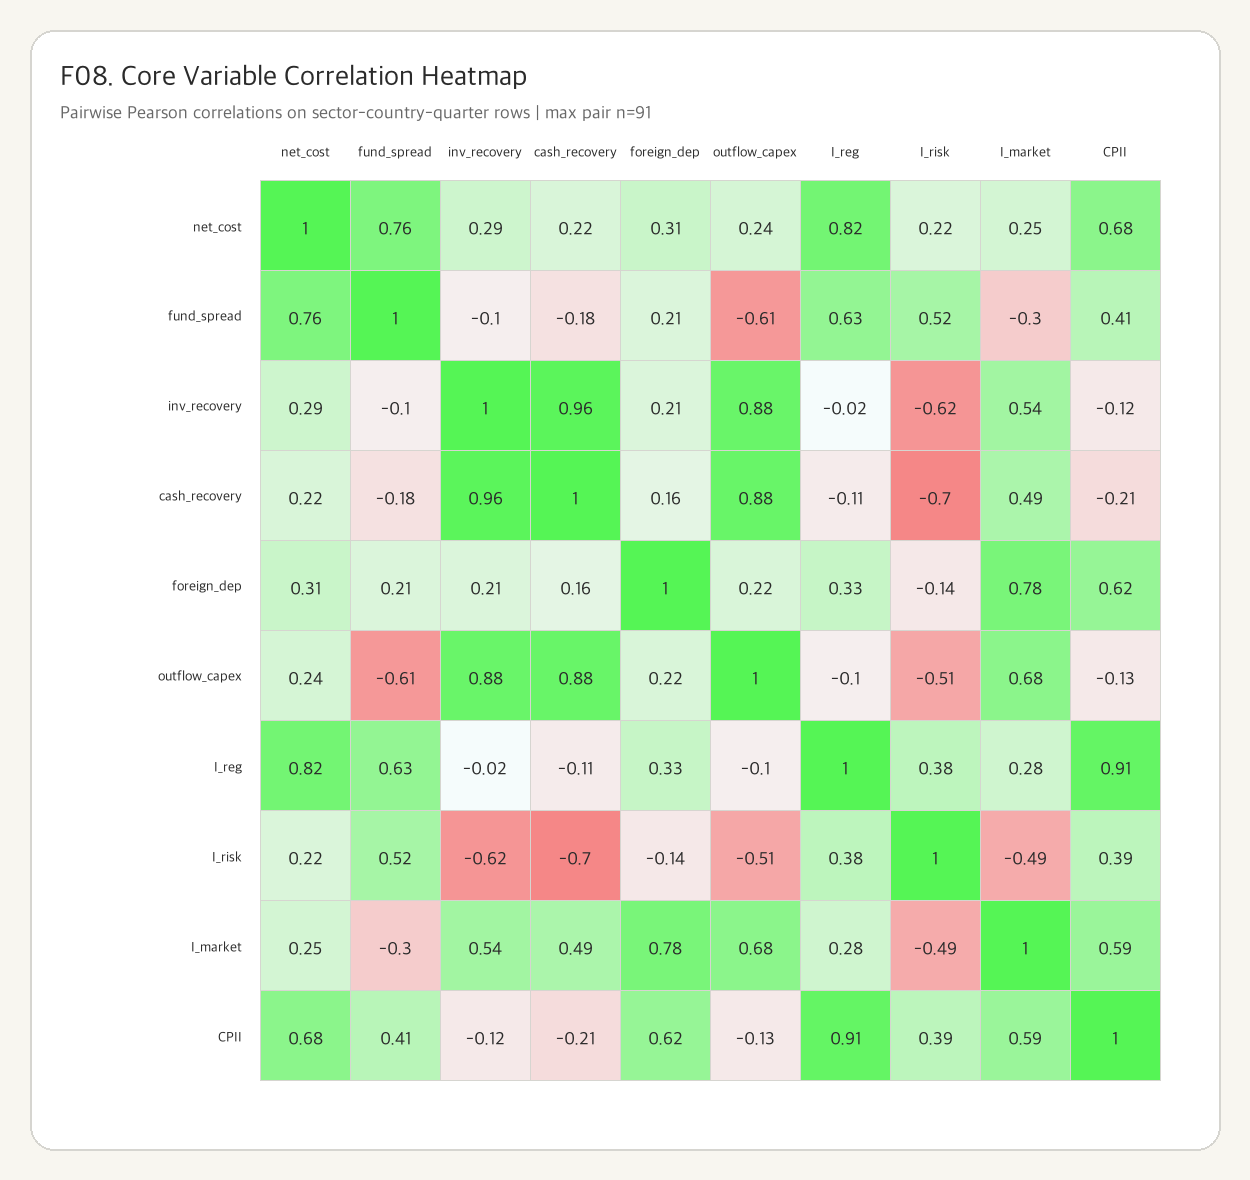
\includegraphics[width=0.92\textwidth]{outputs/figures/F08_core_variable_correlation_heatmap.png}
\caption{핵심 변수 상관구조 히트맵(F08)}
\label{fig:results_corr_heatmap}
\end{figure}

표~\ref{tab:results_basic_stats}에서 가장 큰 분산은 \texttt{investment\_recovery\_ratio}와 \texttt{outflow\_to\_capex\_ratio}에서 확인된다. 플랫폼-월 기준 \texttt{investment\_recovery\_ratio} 평균은 610.16, 표준편차는 1,160.51이었고, 분야-국가-분기 기준 \texttt{outflow\_to\_capex\_ratio} 평균은 108.00, 표준편차는 221.56이었다. 반대로 \texttt{foreign\_dependency\_ratio}는 플랫폼-월 패널에서 평균 0.826, 표준편차 0.073 수준으로 비교적 안정적인 분포를 보였다. 그림~\ref{fig:results_corr_heatmap}은 네트워크 비용, 자금조달 스프레드, 회수율 계열 변수와 하위 지수 및 CPII 사이의 결합구조를 보여주며, 특정 채널이 완전히 동일한 정보를 반복하는 구조는 아님을 확인해 준다.

\section{CPII 산출 결과}
세 분야의 구조적 불평등 수준을 공통 척도인 CPII로 비교하면, 계산 가능한 분야-분기 기준 관측치는 총 14개이며 분야 평균 CPII는 웹툰 및 스토리 54.23, 음악 54.13, 디지털 인프라 43.00으로 나타났다. 다만 식 (5.1)의 세 하위지수인 $I^{\mathrm{reg}}$, $I^{\mathrm{risk}}$, $I^{\mathrm{market}}$가 분야별로 어떤 부담을 의미하는지는 별도로 읽어 줄 필요가 있다. 표~\ref{tab:results_cpii_means}는 각 하위지수의 절대수준(0--100)을 직접 보여 주고, 표~\ref{tab:results_cpii_centered}는 이를 방향 해석이 쉽도록 50을 기준으로 다시 표현한 보조표다. 두 번째 표의 0은 고정 참조분포의 50점 중간점을 옮겨 놓은 산술 기준일 뿐, 정책적 중립점이나 국내기업과 해외기업의 동률을 뜻하지 않는다. 양수와 음수는 각각 이 참조중간점의 위와 아래를 나타내며, 국내외 상대부담은 별도의 동일시장 기업쌍 비교에서 판정해야 한다.

\subsection{공통 관측기간과 분야 순위의 민감도}
분야 평균의 순위는 비교기간을 맞추어 해석해야 한다. 음악의 기존 평균은 6개 분기, 웹툰 및 스토리는 4개 분기, 디지털 인프라는 4개 분기를 사용한다. 세 분야에 모두 값이 있는 기간은 2025년 2--4분기의 3개 분기다. 표~\ref{tab:common_window_revision}는 원래 가용기간 평균을 보존하면서 이 공통기간의 평균을 추가로 계산한 결과다.

\begin{table}[H]
\centering\small
\caption{가용기간 평균과 동일한 3개 분기 평균의 비교}
\label{tab:common_window_revision}
\begin{tabular}{L{3.0cm}rrrrr}
\toprule
\rowcolor{ReportTableHead}
분야 & 가용분기 수 & 기존 CPII & 공통 CPII & 공통 위험 & 공통 시장 \\
\midrule
음악 & 6 & 54.134 & 55.845 & 47.987 & 53.653 \\
웹툰 및 스토리 & 4 & 54.230 & 50.426 & 66.151 & 38.520 \\
디지털 인프라 & 4 & 42.998 & 43.401 & 47.854 & 41.520 \\
\bottomrule
\end{tabular}
{\par\raggedright\footnotesize 주: 공통기간은 2025Q2, 2025Q3, 2025Q4이며 분기별 동일가중 평균이다. 위험과 시장은 각각 해당 기간의 하위지수 평균이다. 분야 점수는 주 분석국가의 가용 국가별 하위지수를 집계한 값이다. 기업·국가 구성은 각 원래 산출행을 유지하였다. 근거: \nolinkurl{data/processed/cpii_panel_sector_quarter.csv}; 검산: \nolinkurl{docs/comprehensive_revision_20261026/sector_common_window_check.csv}.\par}
\end{table}

공통기간에서는 음악이 웹툰 및 스토리보다 5.419점 높다. 따라서 기존 가용기간 평균의 웹툰 1위는 기간 선택에 민감하다. 반면 웹툰의 위험 하위지수가 시장 하위지수보다 높고, 인프라의 위험 하위지수가 가장 높다는 채널별 특징은 유지된다. 음악의 공통기간 제도 하위지수는 65.896점으로 시장 하위지수보다 높아, 음악의 지배적 채널도 기간에 따라 달라진다. 본문의 공통기간 4개 분기 이상 권고에 비추어 이 3개 분기 비교는 탐색적 민감도 점검으로 사용하며, 안정적인 분야 순위에는 추가 공통분기가 필요하다.


\begin{table}[H]
\centering
\small
\caption{하위 지수 분야별 절대수준 표(T09)}
\label{tab:results_cpii_means}
\begin{tabular}{lrrrp{5.6cm}}
\toprule
\rowcolor{ReportTableHead}
분야 & 평균 $I^{\mathrm{reg}}$ & 평균 $I^{\mathrm{risk}}$ & 평균 $I^{\mathrm{market}}$ & 해석 \\
\midrule
웹툰 및 스토리 & 55.224 & 66.956 & 40.509 & 위험 하위지수가 가장 높다. 조달비용·무형자산/매출 격차와 두 회수 대리지표의 결합이며, 정산지연과 실제 창작자 배분률은 활성 입력에 포함되지 않는다. \\
음악 & 54.489 & 46.197 & 61.716 & 시장 하위지수가 가장 높다. 시장전이·해외의존·비용/설비투자 비율의 합성값이며, 번들 요금비율은 시장전이의 구성과 시나리오에 사용된다. \\
디지털 인프라 & 38.365 & 47.865 & 42.764 & 세 채널 모두 다른 두 분야보다 낮지만, 비용회수와 투자여력을 반영하는 $I^{\mathrm{risk}}$가 상대적으로 가장 높다. \\
\bottomrule
\end{tabular}
\end{table}

\begin{table}[H]
\centering
\small
\caption{하위 지수 0기준 상대부담 재표현표(T10)}
\label{tab:results_cpii_centered}
\begin{tabular}{lrrrp{5.6cm}}
\toprule
\rowcolor{ReportTableHead}
분야 & $I^{\mathrm{reg}}-50$ & $I^{\mathrm{risk}}-50$ & $I^{\mathrm{market}}-50$ & 해석 \\
\midrule
웹툰 및 스토리 & +5.224 & +16.956 & -9.491 & 제도 채널과 특히 위험 채널은 고정 참조중간점을 상회하고, 시장 채널은 하회한다. 이 표만으로 국내외 상대적 유불리를 판정하지 않는다. \\
음악 & +4.489 & -3.803 & +11.716 & 제도·시장 채널은 고정 참조중간점을 상회하고 위험 채널은 하회한다. 국내외 비교는 별도 기업쌍 격차를 따른다. \\
디지털 인프라 & -11.635 & -2.135 & -7.236 & 세 채널 모두 고정 참조중간점 아래에 위치한다. 이는 정책적 중립이나 해외기업 대비 유리함을 의미하지 않는다. \\
\bottomrule
\end{tabular}

\vspace{0.3em}
{\par\raggedright\footnotesize 주: 본 표의 값은 각 하위지수 평균에서 고정 참조분포의 중간점 50을 뺀 보조값이다. 0은 산술적 참조중간점일 뿐 정책적 중립, 부담 부재, 국내외 기업의 동률을 뜻하지 않는다. 양수와 음수는 각각 참조중간점의 위와 아래를 표시하며, 국내외 상대부담이나 유불리는 별도의 동일시장 기업쌍 비교에서 판정한다.\par}
\end{table}

\begin{figure}[H]
\centering
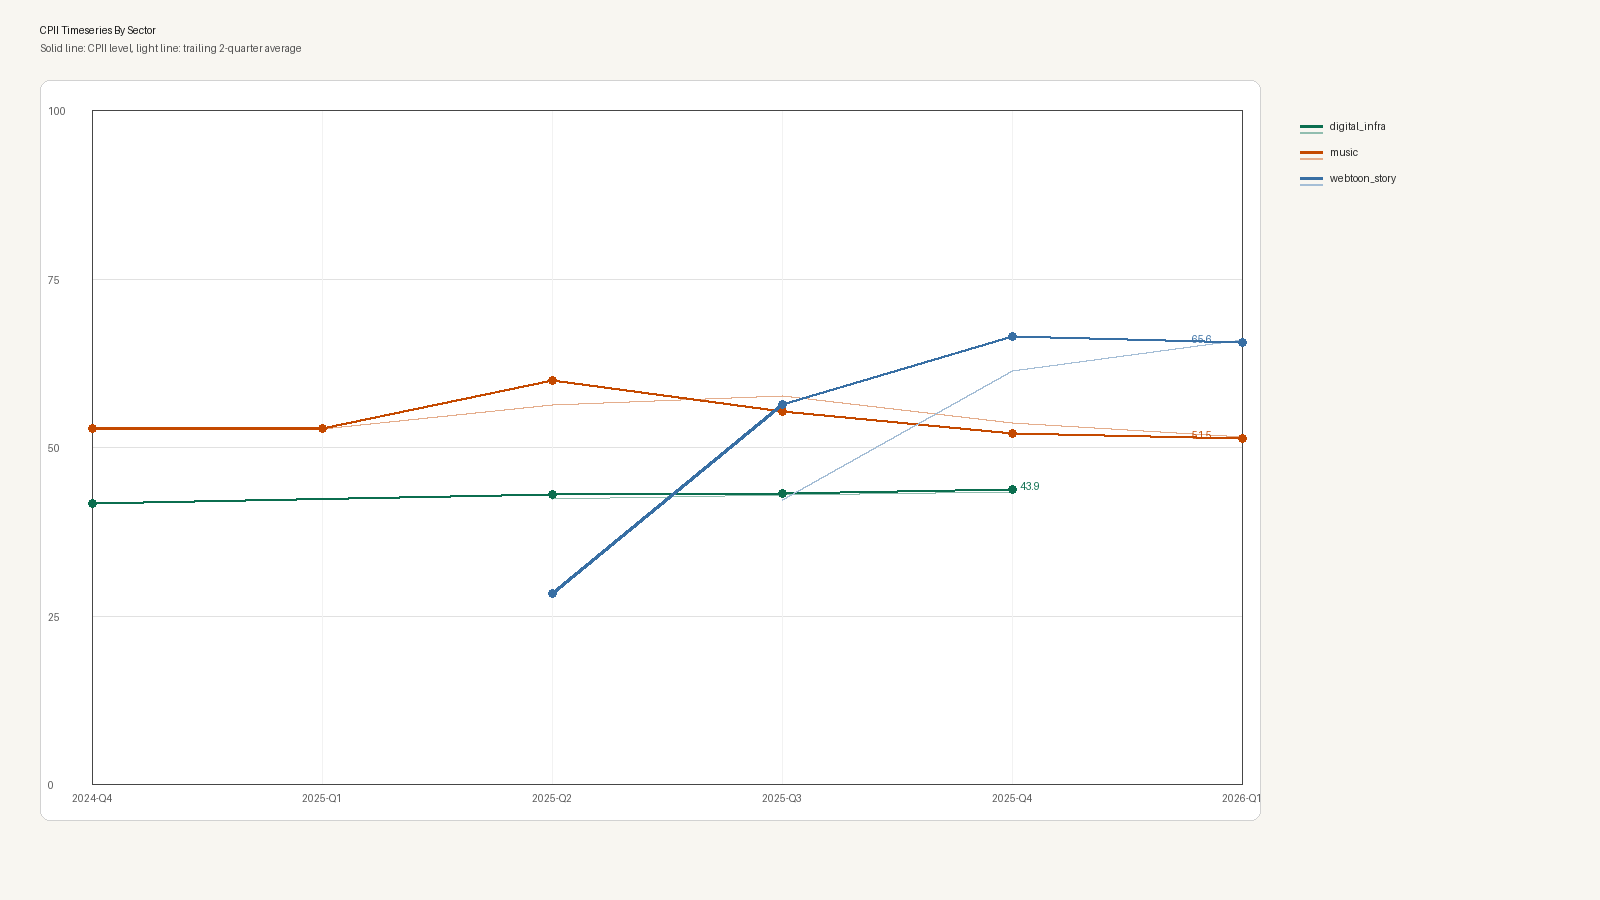
\includegraphics[width=0.92\textwidth]{outputs/figures/cpii_timeseries_by_sector.png}
\caption{CPII 시계열 선그래프(F02)}
\label{fig:results_cpii_timeseries}
\end{figure}

\begin{figure}[H]
\centering
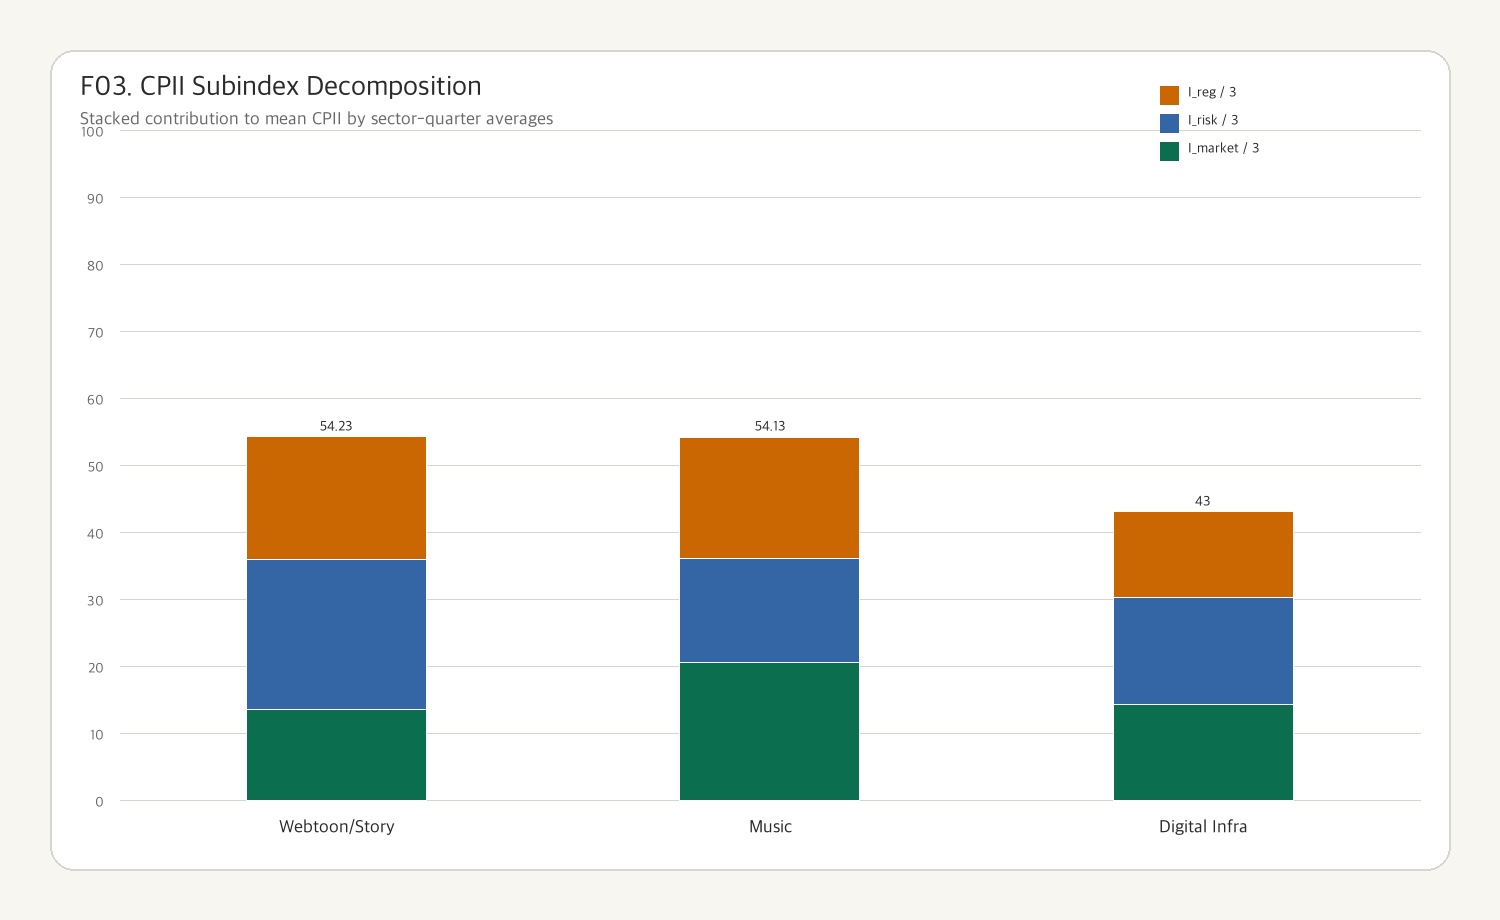
\includegraphics[width=0.92\textwidth]{outputs/figures/F03_cpii_subindex_decomposition.png}
\caption{하위 지수 분해 누적막대그래프(F03)}
\label{fig:results_cpii_decomposition}
\end{figure}

\begin{figure}[H]
\centering
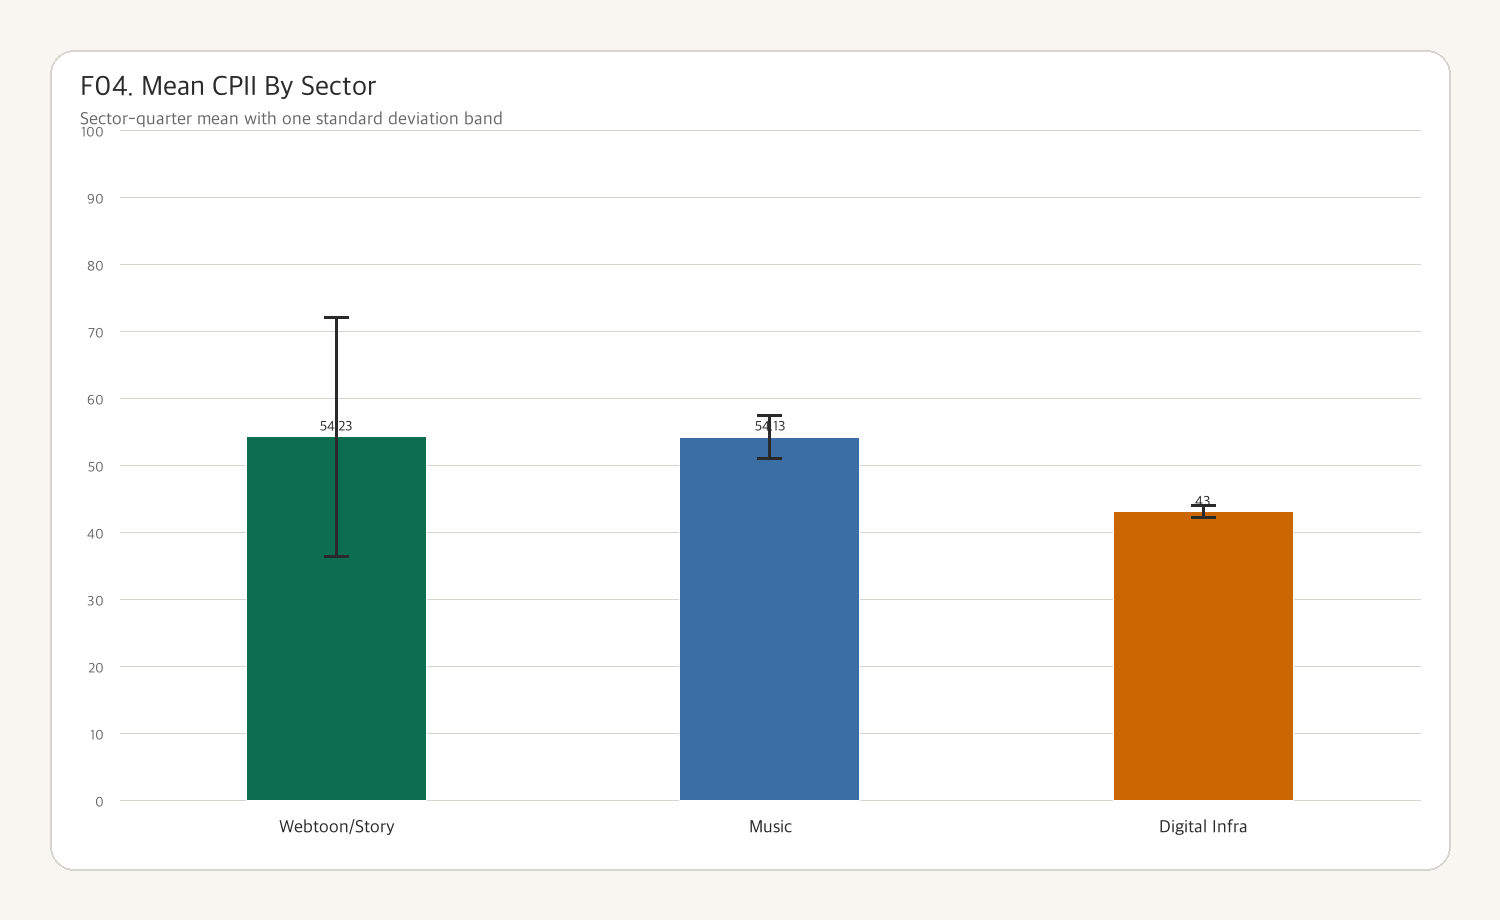
\includegraphics[width=0.92\textwidth]{outputs/figures/F04_cpii_sector_mean_compare.png}
\caption{분야별 평균 비교 막대그래프(F04)}
\label{fig:results_cpii_sector_compare}
\end{figure}

\begin{figure}[H]
\centering
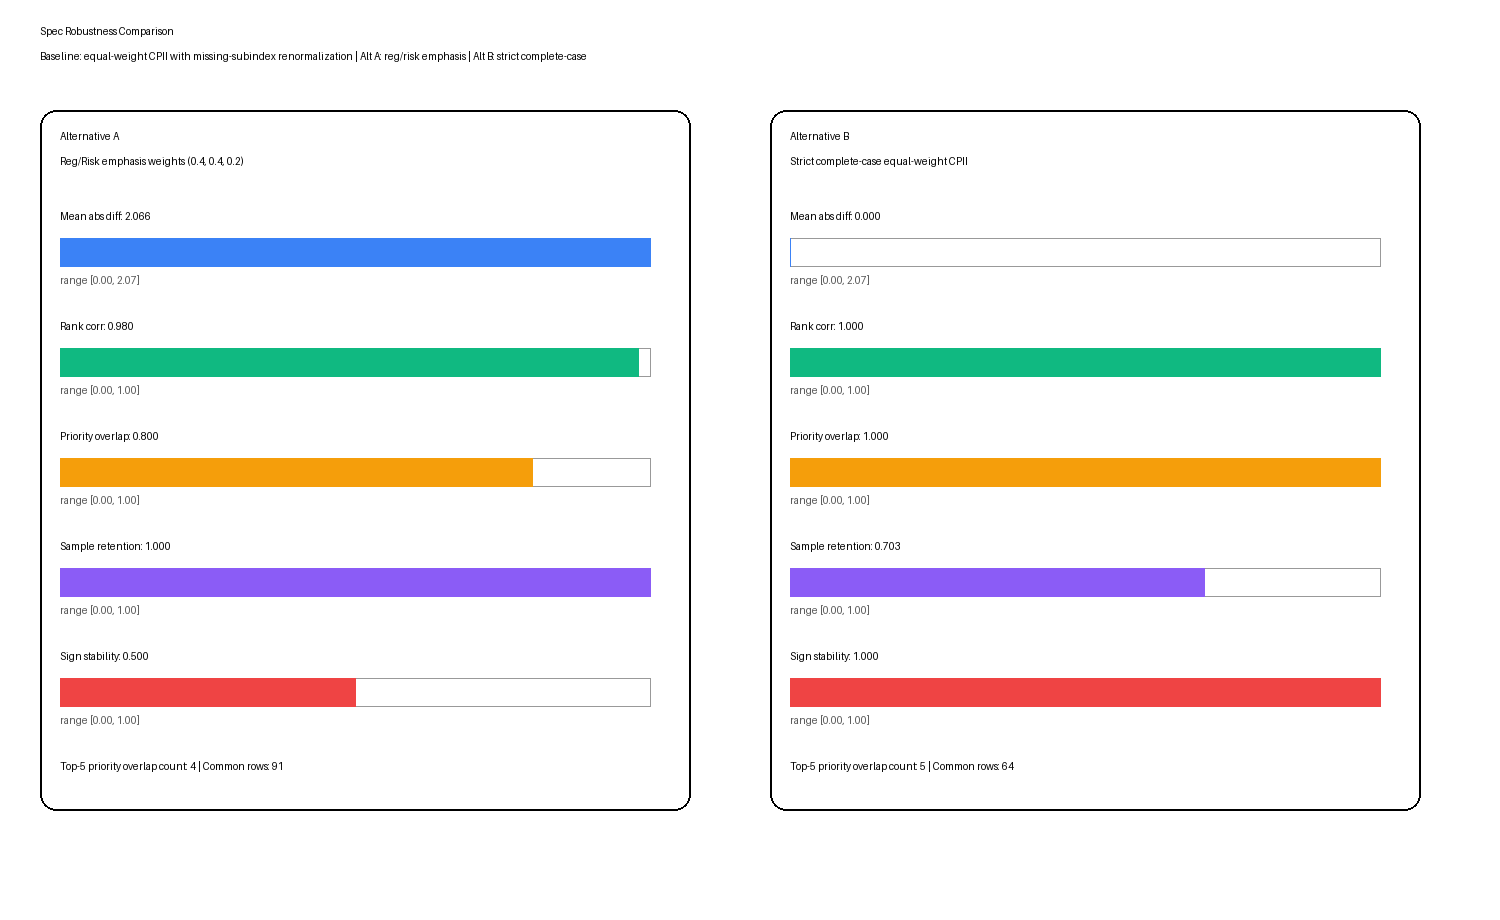
\includegraphics[width=0.92\textwidth]{outputs/figures/spec_comparison_chart.png}
\caption{기준 사양-대체 사양 비교 차트(F09)}
\label{fig:results_cpii_robustness}
\end{figure}

두 표를 함께 읽으면 웹툰 및 스토리는 회수위험과 배분구조 채널, 음악은 시장전이 채널에서 한국 기업의 어려움이 가장 크게 드러난다. 반면 디지털 인프라는 총점 자체가 다른 두 분야보다 낮고, 0기준 보조표에서도 세 하위지수가 모두 고정 참조중간점 아래에 있다. 이는 참조분포상 위치에 관한 기술이지 정책적 중립이나 해외기업 대비 유리함의 판정은 아니다. 극단 관측치를 보면 최고치는 웹툰 및 스토리 2025Q4의 66.49, 최저치는 웹툰 및 스토리 2025Q2의 28.39였다. 국가 비교를 결합하면 전체 관측치 기준 평균 CPII는 영국 65.04, 대만 57.68, 한국 53.67 순으로 높았고, 공통 표본 기준으로도 영국 56.07, 대만 49.86, 한국 47.28 순으로 유지되었다. 강건성 비교에서는 대체 사양 A의 평균 절대 점수차가 2.07점, 순위상관이 0.980으로 나타났고 최신 top-5 정책 우선순위는 5개 중 4개가 유지되었다. 반면 대체 사양 B는 순위상관 1.000과 top-5 완전 일치를 보였지만 sector-country-quarter 표본 유지율이 70.3\%로 축소되었다. 또한 Alt A에서는 공통표본 회귀 기준 $I^{\mathrm{risk}}$의 부호 안정성이 흔들려 channel-level 해석은 더 보수적으로 잡아야 한다. 특히 미국 인프라 FY2024 annual, 한국 통신 3사의 FY2024 annual, 그리고 영국·대만의 2024Q4 공식 국가 proxy를 추가 확보하면서 디지털 인프라 peer set의 공통 기업-분기 구간이 2024Q4--2025Q4의 4개로 늘어났다는 점은 이번 결과 해석의 중요한 전제다. 총점의 절대 수준보다 채널별 기여분과 기준 사양 대비 순위 안정성, 그리고 공통표본의 두께가 더 중요하다.

\begin{table}[H]
\centering
\small
\setlength{\tabcolsep}{3pt}
\caption{결과별 세부 판독 단위}
\label{tab:results_reading_unit}
\begin{tabular}{L{2.4cm}L{2.8cm}L{3.9cm}L{5.0cm}}
\toprule
\rowcolor{ReportTableHead}
결과 묶음 & 1차 요약값 & 함께 볼 세부항목 & 판독 규칙 \\
\midrule
분야 평균 CPII & 분야 평균 총점 & $I^{\mathrm{reg}}, I^{\mathrm{risk}}, I^{\mathrm{market}}$ 분해 & 총점은 수준 비교용 요약값이며, 채널 해석은 하위지수 분해를 함께 봐야 한다. \\
\midrule
한국시장 부담귀착 방향 평균 & 분야별 평균 핵심/확장 방향점수 & 회사별 비교사례, 관측축 수, 자료의 직접성과 비교 가능성 & 분야 평균은 사례의 방향을 요약한다. 개별 비교의 관측 범위와 자료의 직접성을 함께 확인한다. \\
\midrule
정책 시뮬레이션 & 시나리오별 전체 평균 $\Delta \mathrm{CPII}$ & 분야별 정책표, 최신분기 값, 하위지수별 변화 채널 & 전체 평균은 1차 선별용 요약값이며, 실제 정책판단은 분야별 이질성과 어떤 하위지수를 움직이는지까지 같이 봐야 한다. \\
\bottomrule
\end{tabular}
\end{table}

회사별 분석은 부담이 집중되는 기업·서비스 조합을 식별한다. 공시자료가 연결된 기업은 가용기간의 회사 평균 CPII를, 동일시장 사례는 부담귀착 방향점수를 중심으로 비교한다. 다음 절에서는 두 지표의 계산 단위와 회사별 적용 범위를 정리한다.

\section{회사별 사례연구}
한국시장 부담귀착 확장 방향점수의 평균은 음악 0.450833, 웹툰 및 스토리 0.166666, 디지털 인프라 0.482495로 모두 양수다. 이 값은 영(0)을 기준으로 사례별 방향점수를 평균한 것이며, 기업별 판단에는 회사 평균 CPII와 비교쌍의 관측 범위를 함께 사용한다.

회사별 수치쌍 `핵심 / 확장`은 같은 사례행 \(r\)에 대해 계산한 두 종류의 부호형 증거점수 평균이다. `핵심`은 규제 직접부담, 회수위험, 시장전이의 세 축만 평균한 값이고, `확장`은 여기에 `reach`와 `creator`를 더한 값이다. 따라서 예컨대 `0.575 / 0.525`는 첫째 수가 핵심 부호형 증거 평균, 둘째 수가 확장 부호형 증거 평균이라는 뜻이며, 추가된 두 축이 핵심 평균을 끌어내리거나 끌어올릴 수 있다.

`reach`는 같은 서비스·시장에서 신고, 보고, 자료제출, 집행 절차가 국내외 사업자를 포착하는 정도와 그 관측 가능성을 비교한다. 양수는 한국 사업자 쪽 절차상 부담이 더 직접적으로 관측되는 방향이다. 해외 비교기업의 자료가 제한되거나 간접적인 경우에는 그 관측 차이도 함께 반영된다.

`creator`는 창작자 배분률, 총매출 기준 정산, 할인 포함 여부, 이용로그와 감사 대응에 드는 비용이 국내외 사업자에게 어떻게 귀착되는지 비교한다. 양수는 한국 플랫폼 쪽 부담이 더 크다는 뜻이다. 음악은 해당 비용의 직접 관측이 상대적으로 많으며, 웹툰 및 스토리는 유사한 방향을 보이지만 비교자료의 범위가 좁다.

음악의 여섯 비교사례는 모두 국내 부담 방향을 보인다. 산업 전체에 일반화할 근거로 단독 채택하는 내부 기준을 충족한 사례는 0개다. 따라서 회사 평균에 근거한 부담 수준, 동일시장의 부담 방향, 제한된 관측과 부호가 혼합된 사례를 구분하여 제시한다.

아래 표는 회사별 지표와 해석 범위를 정리한다. 회사 평균 CPII(0--100)는 가용 표본기간의 평균 부담을, 한국시장 부담귀착 방향점수($[-1,+1]$, 영(0) 기준)는 같은 시장의 비교쌍에서 부담이 향하는 쪽을 보여 준다. 방향점수와 기업쌍의 CPII 격차는 서로 다른 값이다. WEBTOON Entertainment와 NAVER는 회사 수준 자료를 중심으로, 회사 평균 CPII가 구축되지 않은 Kakao Entertainment / Melon은 서비스별 방향점수를 중심으로 읽는다. Dreamus / FLO 대 Spotify의 확장점수 0.480000은 음악 사례 중 직접 비교자료가 상대적으로 풍부하다. KT 대 Netflix의 확장점수는 0.583669이고, SK Telecom·LG Uplus는 종합점수와 위험-회수 축의 부호가 다르다. KakaoWebtoon 대 WEBTOON, KakaoPage 대 Piccoma는 양수 방향을 보이며 관측축의 추가 확보가 필요하다.

분야별 결과에서는 멜론·FLO의 동일시장 경쟁압력, NAVER·WEBTOON Entertainment와 카카오 계열의 자료 범위 차이, KT와 SK Telecom·LG Uplus의 위험-회수 부호 차이를 패널 결과와 사건연구에 연결해 설명한다.

\begingroup
\footnotesize
\hbadness=10000
\newcommand{\CaseCell}[1]{\WrapCell{#1}}
\setlength{\tabcolsep}{2.5pt}
\setlength{\LTleft}{\fill}
\setlength{\LTright}{\fill}
\captionsetup{hypcap=false}
\captionof{table}{회사별 사례연구 요약표}
\label{tab:firm_case_studies}
\begin{longtable}{@{}L{2.2cm}L{1.45cm}L{3.55cm}L{7.8cm}@{}}
\toprule
\rowcolor{ReportTableHead}
회사(서비스) & 증거 성격 & 핵심 수치 & 읽기 규칙 \\
\midrule
\endfirsthead
\toprule
\rowcolor{ReportTableHead}
회사(서비스) & 증거 성격 & 핵심 수치 & 읽기 규칙 \\
\midrule
\endhead
\multicolumn{4}{@{}l@{}}{\textbf{음악}} \\
\midrule
\CaseCell{카카오엔터테인먼트\\/ Melon} & \CaseCell{부담귀착 방향\\사례 중심} & \CaseCell{회사 평균 CPII 미구축\\vs Spotify 0.500 / 0.538\\vs YouTube Music 0.575 / 0.525\\vs Apple Music 0.400 / 0.413} & 회사 평균 CPII는 구축되지 않았으며, 한국시장 서비스 비교의 방향점수는 반복적으로 양수다. 해석은 해당 비교사례의 범위에 적용한다. \\
\midrule
\CaseCell{Dreamus\\/ FLO} & \CaseCell{회사 평균 +\\부담귀착 방향 사례} & \CaseCell{평균 CPII 65.29\\vs Spotify 0.417 / 0.480\\vs Apple Music 0.350 / 0.388} & 회사 평균 CPII와 서비스별 부담 방향을 함께 확인할 수 있다. FLO 대 Spotify는 음악 사례 중 직접 비교자료가 상대적으로 풍부하다. \\
\midrule
\CaseCell{구글\\(Alphabet / YouTube)} & \CaseCell{해외\\비교군} & \CaseCell{Alphabet 평균 CPII 41.05\\Melon vs YouTube Music 0.575 / 0.525\\Melon vs Premium Lite 0.425 / 0.363\\조건부 유료 진입가격 차이 $-3{,}490$원} & 인프라 기준 평균 부담은 한국 통신 3사보다 낮지만, 한국 음악시장에서는 YouTube 번들과 Premium Lite가 가장 강한 가격·진입 압력 사례다. \\
\midrule
\CaseCell{애플\\(Apple Music)} & \CaseCell{보조\\비교군} & \CaseCell{회사 평균 CPII 미구축\\Melon vs Apple Music 0.400 / 0.413} & 한국 음악시장 비교사례는 양수 방향이며, Apple Music 서비스의 회사 평균 CPII를 산출할 직접 연결자료는 확보되지 않았다. \\
\midrule
\multicolumn{4}{@{}l@{}}{\textbf{웹툰 및 스토리}} \\
\midrule
\CaseCell{WEBTOON\\Entertainment} & \CaseCell{회사 평균\\중심} & \CaseCell{평균 CPII 71.24\\$I_{\mathrm{reg}}$ 87.79\\$I_{\mathrm{risk}}$ 62.43\\공통기간 비교군 격차 $+20.03$} & 네이버 계열 글로벌 웹툰 축에서 가장 높은 평균 부담을 보인다. 규제와 리스크가 모두 높아 웹툰 분야 회사 수준 최고 부담 사례로 읽힌다. \\
\midrule
NAVER & \CaseCell{회사 평균\\중심} & \CaseCell{평균 CPII 50.35\\$I_{\mathrm{risk}}$ 73.54\\공통기간 비교군 격차 $-16.33$} & 웹툰 및 스토리에서 평균 부담이 중간 이상이며, 특히 회수위험과 배분구조를 묶은 $I_{\mathrm{risk}}$가 높다. 2025Q3--2026Q1에서 NAVER 54.914, WEBTOON Ent 71.244로, 같은 기간 차이는 $-16.330$점이다. \\
\midrule
\CaseCell{KakaoWebtoon\\/ KakaoPage} & \CaseCell{관측축이 제한된\\방향 사례} & \CaseCell{KakaoWebtoon vs WEBTOON 0.150 / 0.200\\KakaoPage vs Piccoma 0.100 / 0.133} & 카카오 관련 웹툰 사례는 양수 방향이다. 관측축은 핵심 1/3, 확장 3/5이며 대리지표를 포함하므로, 해당 비교 범위에서 해석한다. \\
\midrule
\multicolumn{4}{@{}l@{}}{\textbf{디지털 인프라}} \\
\midrule
KT & \CaseCell{회사 평균 +\\직접 사례} & \CaseCell{평균 CPII 54.72\\$I_{\mathrm{risk}}$ 77.09\\vs Netflix 0.501 / 0.584} & 통신 3사 중 직접 비교의 양수 방향이 가장 뚜렷하다. 높은 $I_{\mathrm{risk}}$는 비용회수와 투자여력을 우선 점검할 근거다. \\
\midrule
SK Telecom & \CaseCell{혼합형 직접\\사례} & \CaseCell{평균 CPII 45.66\\$I_{\mathrm{risk}}$ 50.90\\vs Netflix 0.228 / 0.402} & 종합 방향점수는 양수이며 KT보다 낮다. 직접 위험-회수 축은 음수이므로 종합점수와 해당 축을 나누어 해석한다. \\
\midrule
LG Uplus & \CaseCell{평균 점수 높음\\+ 혼합 사례} & \CaseCell{평균 CPII 75.57\\$I_{\mathrm{reg}}$ 80.81\\$I_{\mathrm{risk}}$ 76.01\\vs Netflix 0.318 / 0.462} & 한국 통신 3사 중 평균 CPII가 가장 높다. Netflix와의 종합 방향점수는 양수이며 KT보다 낮고, 직접 위험-회수 축은 음수다. \\
\midrule
넷플릭스 & \CaseCell{해외\\비교군} & \CaseCell{평균 CPII 48.44\\KT 0.501 / 0.584\\SK Telecom 0.228 / 0.402\\LG Uplus 0.318 / 0.462} & 한국 통신 3사의 주요 해외 비교군이다. 세 회사의 종합 방향점수는 양수다. 직접 위험-회수 축은 KT에서 양수, SK Telecom·LG Uplus에서 음수이므로 기업별 부담 경로를 구분한다. \\
\bottomrule
\multicolumn{4}{@{}p{15.6cm}@{}}{\raggedright\footnotesize 주: 회사 평균 CPII는 0--100 척도이며 높을수록 평균 구조적 부담이 크다는 뜻이다. 부담귀착 부호형 증거점수는 영(0)을 기준으로 하는 $[-1,+1]$ 척도다. 양수는 국내 사업자 쪽, 음수는 해외 비교기업 쪽 부담이 더 크게 관측되는 방향이며 0은 뚜렷한 방향이 없음을 뜻한다. 이는 0--100 CPII와 활성 변수로 계산한 기업쌍 CPII 격차와 서로 다른 값이다. `증거 성격`은 가용 표본기간 평균 부담 근거, 동일시장 부담귀착 방향 사례연구, 보조 비교군, 혼합형 직접 사례를 빠르게 구분하기 위한 표식이다. `회사 평균 CPII 미구축`은 현재 공개 자산으로 직접 공시 연결고리를 만들지 못한 경우다.}
\end{longtable}
\endgroup

음악은 여섯 비교사례에서 국내 부담 방향이 반복된다. 직접 관측과 대리지표가 함께 포함된 사례분석이므로, 산업 평균에 대한 일반화는 개별 서비스의 계약·비용 관측을 확대해 확인한다.

멜론은 한국시장 내 서비스 간 경쟁압력을 중심으로 분석한다. Kakao Entertainment는 직접 공시 연결고리가 없어 회사 평균 CPII가 비어 있지만, Melon 대 Spotify는 0.500 / 0.538, Melon 대 YouTube Music은 0.575 / 0.525, Melon 대 Apple Music은 0.400 / 0.413으로 모두 양수다. 여기서 주요 기준점은 YouTube Music 비교이고, YouTube Premium Lite 0.425 / 0.363과 조건부 유료 진입가격 차이 $-3{,}490$원은 번들형 저가 진입 압력을 보강한다. Apple Music 0.400 / 0.413은 방향은 같지만 보조 비교군에 머문다.

Dreamus / FLO는 회사 재무자료와 동일시장 부담귀착 사례를 함께 확인할 수 있는 음악 비교대상이다. Dreamus 평균 CPII는 65.29, Spotify는 49.63이며, FLO 대 Spotify의 0.417 / 0.480은 핵심·확장 축이 모두 관측된 비교사례다. 음악의 상품 비교에서는 Spotify의 단독 유료 구독과 무료 진입을 구분하고, NAVER 제휴를 통한 결합상품 경로도 포함해야 한다. YouTube Music은 영상·음악 결합상품, Premium Lite는 비음악 동영상 진입상품으로 별도 분류한다. 구체적인 멜론--스포티파이 비교는 제~\ref{sec:melon_spotify_comprehensive}절에서 다룬다.

웹툰 및 스토리는 회사별 자료 범위의 차이가 크다. NAVER와 WEBTOON Entertainment는 회사 평균 CPII를 산출할 재무자료가 연결되어 있다. 카카오 계열은 현재 한국 관련 서비스의 부담귀착 방향 사례를 중심으로 비교한다.

WEBTOON Entertainment는 회사 평균 CPII가 높은 웹툰 비교대상이다. 평균 CPII 71.24, $I_{\mathrm{reg}}$ 87.79, $I_{\mathrm{risk}}$ 62.43, 공통기간 비교군 격차 $+20.03$이 모두 높은 부담 방향을 가리킨다. NAVER도 평균 CPII 50.35와 $I_{\mathrm{risk}}$ 73.54로 강한 부담 근거이지만, 공통기간 비교군 격차 $-16.33$은 2025Q3--2026Q1의 NAVER 54.914와 WEBTOON Entertainment 71.244의 차이다. WEBTOON Entertainment의 $+20.03$은 NAVER·키다리스튜디오 평균 51.217을 뺀 값으로 비교군이 다르다. KakaoWebtoon 대 WEBTOON 0.150 / 0.200, KakaoPage 대 Piccoma 0.100 / 0.133은 모두 양수이며, 관측된 핵심 축은 1개다. NAVER·WEBTOON Entertainment의 회사 평균과 카카오 계열의 대리지표 기반 방향사례를 구분하면, 재무상 부담 수준과 서비스별 경쟁압력을 각각 확인할 수 있다.

디지털 인프라의 회사 사례는 회사 수준 부담과 직접 동일시장 사례가 서로 다른 정보를 준다는 점이 핵심이다. 평균만 보면 LG Uplus 평균 CPII 75.57이 가장 높고, KT 54.72, SK Telecom 45.66, Netflix 48.44 순이다. Akamai 43.97, Alphabet 41.05, Amazon 37.79, Cloudflare 31.87를 함께 놓으면 한국 통신 3사의 평균 부담이 더 높게 보이지만, 이 평균 비교만으로 직접 동일시장 부담까지 같은 강도로 읽을 수는 없다.

직접 사례연구의 주요 기준점은 KT다. KT 대 Netflix는 핵심/확장 부호형 증거점수가 0.500504 / 0.583669로 현재 인프라 축에서 가장 강한 직접 양수 사례이고, $I_{\mathrm{risk}}$도 77.09로 높다. 반면 SK Telecom은 0.227993 / 0.401996, LG Uplus는 0.317729 / 0.461819로 종합 부호형 증거점수는 양수지만, 직접 위험-회수 항목이 각각 $-0.294013$, $-0.114542$로 음수다. 특히 LG Uplus는 평균 부담은 가장 높지만 직접 사례 강도는 KT보다 약하다. 인프라 비교에서는 KT의 종합점수와 위험-회수 축이 모두 양수인 반면, SK Telecom·LG Uplus는 두 지표의 부호가 다르다는 점을 함께 확인해야 한다.

\noindent{\small 근거: 표~\ref{tab:signed_korea_market_case_studies}, 표~\ref{tab:firm_case_studies}.}\\
재현 산출물: \texttt{firm\_comparison\_summary.csv}, \texttt{T\_signed\_korea\_market\_case\_studies.csv}, \texttt{premium\_lite\_did\_results.csv}.

이하에서는 회사별 비교결과를 분야별 사건연구 표본, 패널 추정치, 하위지수 구성에 연결한다.

\subsection{한국시장 비교사례의 점수와 관측 범위}
비교사례의 기본 원칙은 동일 서비스·동일 시장이지만, 저장된 카카오페이지--Piccoma 행은 한국 관련 IP·상품을 서로 다른 시장에서 비교한 보조사례다. 따라서 이 행의 0.100/0.133은 동일한 한국 내 거래조건의 직접 비교와 구분한다. 또한 기업 등록국, 서비스 시장국, 기업집단의 지배관계는 별도 분류다. 미국 등록 WEBTOON Entertainment와 일본 등록 Piccoma라는 분류만으로 각각 한국 기업집단과 독립된 외국 소유 비교기업이라고 간주하지 않는다. 아래 분야 평균은 이 사례 구성을 유지한 연구용 요약값이다.

표~\ref{tab:signed_korea_market_case_studies}는 저장된 11개 사례를 빠짐없이 제시한다. 핵심 점수는 규제·위험·시장 축 중 관측된 값의 평균이고, 확장 점수는 규제 포착범위와 창작자 보호비용 귀착 축을 더한 관측값 평균이다. 각 관측 수의 분모는 핵심 3축과 확장 5축이다. 점수와 관측 범위를 함께 읽어야 멜론--스포티파이의 2축·4축 비교를 FLO--스포티파이의 3축·5축 비교와 구별할 수 있다.
\begin{table}[H]
\centering
\footnotesize
\setlength{\tabcolsep}{3pt}
\caption{한국시장 부담귀착 방향: 전체 11개 비교사례와 관측축 수}
\label{tab:signed_korea_market_case_studies}
\begin{tabular}{@{}L{4.5cm}rrccL{3.8cm}@{}}
\toprule
\rowcolor{ReportTableHead}
비교사례 & 핵심 & 확장 & 핵심 관측 & 확장 관측 & 주요 판독 조건\\
\midrule
멜론 대 스포티파이 & 0.500 & 0.538 & 2/3 & 4/5 & 위험 축 결측 \\
FLO 대 스포티파이 & 0.417 & 0.480 & 3/3 & 5/5 & 5축 관측; 대리측정 포함 \\
멜론 대 YouTube Music & 0.575 & 0.525 & 2/3 & 4/5 & 위험 축 결측 \\
멜론 대 YouTube Premium Lite & 0.425 & 0.363 & 2/3 & 4/5 & 위험 축 결측 \\
멜론 대 Apple Music & 0.400 & 0.413 & 2/3 & 4/5 & 위험 축 결측 \\
FLO 대 Apple Music & 0.350 & 0.388 & 2/3 & 4/5 & 위험 축 결측 \\
\midrule
카카오웹툰 대 WEBTOON & 0.150 & 0.200 & 1/3 & 3/5 & 핵심 시장축만 관측 \\
카카오페이지 대 Piccoma & 0.100 & 0.133 & 1/3 & 3/5 & 서로 다른 시장의 보조사례 \\
\midrule
SK Telecom 대 Netflix & 0.228 & 0.402 & 2/3 & 3/5 & 위험 축 음수 \\
KT 대 Netflix & 0.501 & 0.584 & 2/3 & 3/5 & 위험 축 양수 \\
LG Uplus 대 Netflix & 0.318 & 0.462 & 2/3 & 3/5 & 위험 축 음수 \\
\bottomrule
\end{tabular}
\par\smallskip
\begin{minipage}{\linewidth}
\footnotesize\raggedright 주: 점수 범위는 \([-1,1]\)이며 양수는 국내 사업자 쪽 부담 방향이다. 결측축은 평균에서 제외한다. 관측축 수는 자료 직접성이나 정확성을 대신하지 않는다. 카카오페이지--Piccoma 행은 교차시장 보조사례이며 나머지 행도 관측범위가 제한된 사례연구다. 따라서 개별 기업의 위법성이나 산업 전체 평균의 추정치를 제공하지 않는다. YouTube Premium Lite 행은 음악 단독상품의 동등기능 비교가 아니라 동영상 광고 제거 상품을 통한 진입가격·결합상품 압력의 보조 비교다. 자료: \nolinkurl{outputs/tables/claim_strengthening/signed_rebuild/T_signed_korea_market_case_studies.csv}. 표는 저장된 6자리 값으로부터 반올림했다.
\end{minipage}
\end{table}

표~\ref{tab:signed_case_axes_complete}는 종합점수를 구성하는 다섯 축의 값을 보여준다. 규제 포착범위 축과 규제 직접부담 축의 중첩 가능성은 별도 민감도 분석에서 점검하며, 인프라의 음의 위험 축도 그대로 제시한다.
\begin{table}[H]
\centering
\footnotesize
\setlength{\tabcolsep}{3pt}
\caption{전체 비교사례의 축별 방향점수}
\label{tab:signed_case_axes_complete}
\begin{tabular}{@{}L{4.8cm}rrrrr@{}}
\toprule
\rowcolor{ReportTableHead}
비교사례 & 규제 & 위험 & 시장 & 포착범위 & 창작자 비용\\
\midrule
멜론 대 스포티파이 & 0.750 & --- & 0.250 & 0.500 & 0.650 \\
FLO 대 스포티파이 & 0.750 & 0.500 & 0.000 & 0.500 & 0.650 \\
멜론 대 YouTube Music & 0.500 & --- & 0.650 & 0.400 & 0.550 \\
멜론 대 YouTube Premium Lite & 0.250 & --- & 0.600 & 0.300 & 0.300 \\
멜론 대 Apple Music & 0.500 & --- & 0.300 & 0.350 & 0.500 \\
FLO 대 Apple Music & 0.500 & --- & 0.200 & 0.350 & 0.500 \\
\midrule
카카오웹툰 대 WEBTOON & --- & --- & 0.150 & 0.250 & 0.200 \\
카카오페이지 대 Piccoma & --- & --- & 0.100 & 0.150 & 0.150 \\
\midrule
SK Telecom 대 Netflix & 0.750 & -0.294 & --- & 0.750 & --- \\
KT 대 Netflix & 0.750 & 0.251 & --- & 0.750 & --- \\
LG Uplus 대 Netflix & 0.750 & -0.115 & --- & 0.750 & --- \\
\bottomrule
\end{tabular}
\par\smallskip
\begin{minipage}{\linewidth}
\footnotesize\raggedright 주: ---는 결측이며 0.000은 관측된 중립 방향값이다. 값은 원천 사례표의 \nolinkurl{construction_note}에서 추출했다. 축별 값은 공개자료를 연구의 코딩규칙으로 변환한 방향점수이며, 비용률·회귀계수·유의확률과 구별한다. 이 표의 반올림값으로 재평균할 경우 앞 표와 마지막 자리가 다를 수 있다.
\end{minipage}
\end{table}

\section{음악 분야 결과}
음악 분야의 핵심 결과는 국내 플랫폼의 부담 방향이 복수 비교사례에서 반복된다는 점이다. 표~\ref{tab:firm_case_studies}의 Melon·FLO와 Spotify·YouTube Music·Apple Music 비교를 수요자료와 패널 추정으로 살펴본다. 2025년 5월 WiseApp/Retail 공통 관측값에서 한국 월간 이용자는 유튜브 뮤직 약 982만 명, 멜론 약 654만 명, 스포티파이 약 359만 명이었다. 기준 FE 패널의 \texttt{foreign\_dependency\_ratio} 계수는 유의하지 않았고, \texttt{Spotify Lossless} 도입 사건의 stacked event study는 사전추세 검정을 통과하지 못했다. 따라서 표~\ref{tab:results_music_estimates}는 사건 전후 차이와 식별조건을 점검하는 자료로 사용하며, 부담 방향에 관한 판단은 서비스별 비교사례와 수요·가격·정산자료에 근거한다.\sourcefootnote{\srcKJADMusic, \srcChosunBizMusic}

\begin{table}[H]
\centering
\small
\caption{음악 분야 사건연구 및 강건성 추정치 요약표(T11-Music)}
\label{tab:results_music_estimates}
\begin{tabular}{llrrrrr}
\toprule
\rowcolor{ReportTableHead}
모형 & 설명변수 & N & 계수 & 표준오차 & $p$값 & 사전추세 \\
\midrule
FE panel & \texttt{foreign\_dependency\_ratio} & 231 & 82.385 & 217.277 & 0.705 & not applicable \\
Event study & \texttt{treated\_rel\_m2} & 1190 & 446.731 & 32.550 & 0.000 & fail \\
Event study & \texttt{treated\_rel\_p0} & 1190 & 446.731 & 32.550 & 0.000 & fail \\
Event study & \texttt{treated\_rel\_p1} & 1190 & -275.617 & 23.027 & 0.000 & fail \\
Event study & \texttt{treated\_rel\_p2} & 1190 & -275.617 & 23.027 & 0.000 & fail \\
Event study & \texttt{treated\_rel\_p3} & 1190 & -275.617 & 23.027 & 0.000 & fail \\
Event study & \texttt{treated\_rel\_p4} & 1190 & -275.617 & 23.027 & 0.000 & fail \\
Event study & \texttt{treated\_rel\_p5} & 1190 & -275.617 & 23.027 & 0.000 & fail \\
\bottomrule
\end{tabular}
\end{table}

\begin{figure}[H]
\centering
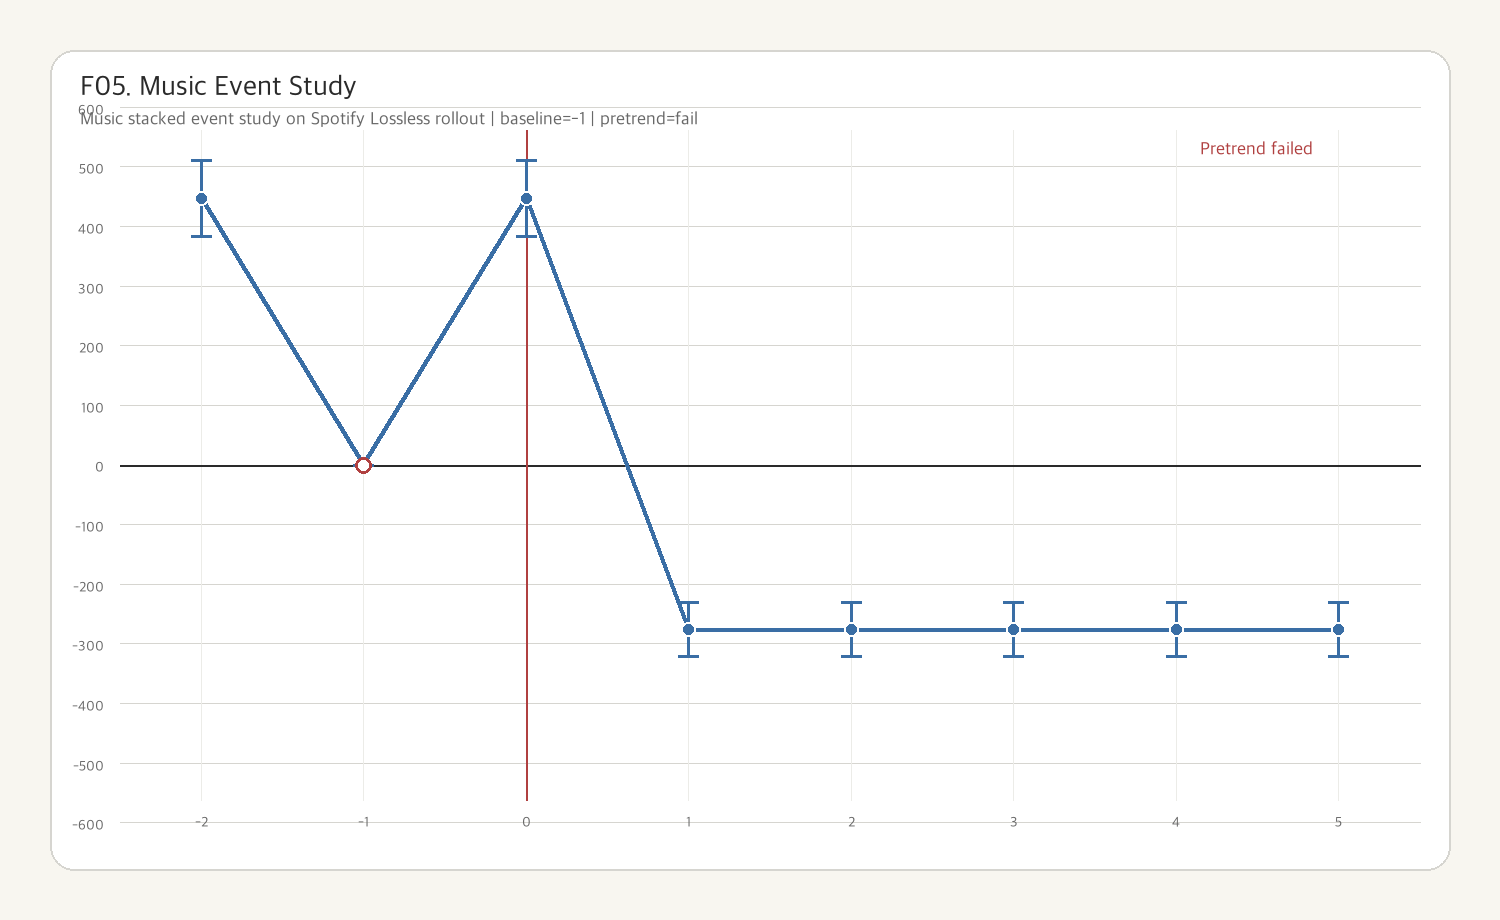
\includegraphics[width=0.92\textwidth]{outputs/figures/F05_music_event_study_plot.png}
\caption{음악 분야 사건 전후 변화 그래프(F05)}
\label{fig:results_music_event}
\end{figure}

음악 분야의 CPII는 2025Q2에 60.07로 가장 높았고, 2025Q3--2026Q1에는 51.47--55.39였다. 회사별 자료와 서비스 비교에서는 Dreamus 및 Melon·FLO 사례가 국내 부담 방향을 뒷받침한다(표~\ref{tab:firm_case_studies}). 사건연구의 사전추세 위반은 별도로 고려해야 하므로, 이하에서는 상품 가격, 국내 제휴, 이용자 기반과 정산구조를 중심으로 이 부담이 형성되는 경로를 분석한다.

\section{멜론과 스포티파이: 동일시장 경쟁과 카카오엔터테인먼트의 대응}
\label{sec:melon_spotify_comprehensive}

멜론과 스포티파이의 비교는 국내 음악 구독자의 선택, 플랫폼의 비용회수, 콘텐츠 유통수익이라는 세 가지 의사결정을 연결한다. 이용자는 곡목과 추천 품질, 이용기기, 오프라인 재생, 구독료와 제휴혜택을 함께 고려한다. 멜론의 운영성과를 평가하려면 이 선택이 유료가입 유지와 이용자당 수익에 어떤 변화를 만드는지 관측해야 한다. 카카오엔터테인먼트 차원에서는 멜론의 구독사업과 음원 제작·유통사업의 성과를 함께 살펴야 한다. 해외 서비스의 이용 확대가 멜론의 구독 경쟁을 높이는 동시에 유통 음원의 해외 수익기회를 넓힐 수 있기 때문이다. 어느 효과가 더 큰지는 사업별 현금흐름과 계약조건에 따라 달라진다.

이 절은 프로젝트에 보존된 2025년 수요자료, 2026년 3월 가격자료와 기존 부담귀착 점수를 먼저 비교한다. 여기에 공식 발표에서 확인한 네이버 제휴와 서비스 연결 구조를 보완한다. 서로 다른 기준시점은 표와 본문에 표시하며, 추가로 확인한 제휴 사실을 기존 점수에 소급 반영하지 않는다. 이 구분을 통해 기존 분석의 재현성을 유지하면서 경영진이 검토해야 할 경쟁경로를 넓힌다.

\subsection{비교 단위: 멜론 서비스, 카카오엔터테인먼트, 스포티파이 연결실적}

멜론은 한국 소비자가 이용하는 음악 서비스이고, 카카오엔터테인먼트는 여러 콘텐츠 사업을 수행하는 법인이다. 스포티파이의 연결실적 역시 한국 유료 음악서비스만의 실적과 범위가 다르다. 따라서 한국 서비스의 가격·가입자·이용시간은 같은 한국 시장의 서비스끼리 비교하고, 재무비율은 회계기간·연결범위·수익구성을 확인한 기업 자료끼리 비교해야 한다. 법인 전체의 세율이나 이익률을 한국 음악서비스의 비용으로 배분하려면 별도 배분근거가 필요하다.

현재 회사별 집계표에서 카카오엔터테인먼트의 회사 평균 CPII는 미구축이다. 스포티파이의 49.63은 2025년 3분기부터 2026년 1분기까지 3개 분기와 9개 시장에 연결된 가용항목 집계값이다. 이 숫자에서 멜론의 부담 수준을 역산할 수 있는 연결고리는 아직 없다. 멜론--스포티파이 비교에 직접 사용할 수 있는 기존 결과는 뒤에서 설명하는 핵심 0.5000, 확장 0.5375의 한국시장 사례점수다. 회사 평균, 같은 시장의 서비스 비교, 사례점수라는 세 층위를 구분하면 자료의 빈칸을 다른 사업의 숫자로 채우는 오류를 줄일 수 있다.

\subsection{가격과 상품 구성: 정가 동률 이후의 경쟁}

표~\ref{tab:melon_spotify_prices_20261026}은 기존 가격패널의 월 정기결제 상품을 기능별로 대응시킨다. 멜론 스트리밍클럽과 Spotify Premium Basic은 각각 월 8,690원이며, 멜론 스트리밍 플러스와 Spotify Premium 개인은 각각 월 11,990원이다. 같은 기능 묶음 안의 정가 차이는 두 비교 모두 0원이다. 따라서 기존 관측시점의 경쟁압력은 ``해외 서비스의 단독 정가가 더 싸다''는 설명만으로 파악되지 않는다. 무료 진입, 할인 자격, 제휴상품, 추천과 탐색의 편의성을 함께 보아야 한다.

\begin{table}[H]
\centering\setlength{\tabcolsep}{3pt}
\small
\caption{멜론과 스포티파이의 한국 월 정기결제 가격 비교}
\label{tab:melon_spotify_prices_20261026}
\begin{tabular}{L{2.6cm}L{3.5cm}L{3.4cm}L{4.8cm}}
\toprule
\rowcolor{ReportTableHead}
비교 기준 & 멜론 & 스포티파이 & 해석 및 이용 조건 \\
\midrule
온라인 음악감상 & 스트리밍클럽 8,690원 & Premium Basic 8,690원 & 정가 동일. Basic은 음악 다운로드를 제공하지 않는다. \\
오프라인 음악감상 포함 & 스트리밍 플러스 11,990원 & Premium 개인 11,990원 & 정가 동일. 저장기기·음질 등 세부조건은 상품별로 확인한다. \\
이용범위 제한 할인 & 모바일 스트리밍클럽 7,590원 & Premium 학생 6,600원 & 전자는 기기 범위, 후자는 학생 자격 조건이 있어 할인액을 직접 대응시키기 어렵다. \\
복수 계정 & 이 표의 공통 대응상품 미설정 & Premium Duo 17,985원 & 같은 주소지의 두 계정 조건. 두 계정을 모두 쓰면 계정당 8,992.5원이다. \\
\bottomrule
\end{tabular}
\par\smallskip
\begin{minipage}{0.96\linewidth}\footnotesize
주: 원/월, 부가세 포함. 기준자료는 프로젝트에 2026년 3월로 기록된 공식 가격표 스냅샷이며, 일회성 체험·프로모션은 제외하였다. 온라인/오프라인 기능 구분은 비교를 위한 최소 기준이고 모든 품질의 동일성을 뜻하지 않는다. 2026년 10월 26일 확인한 양사 공식 페이지에서도 위 가격을 확인하였다. 원천: \nolinkurl{platform_product_price_panel.csv}, 멜론 전체 이용권 및 Spotify 대한민국 Premium 안내.
\end{minipage}
\end{table}

스포티파이의 공식 국내 안내는 무료 이용과 Premium을 구분한다. 광고 기반 무료 이용은 최초 가입의 현금 부담을 낮출 수 있지만, 유료가입자당 수익과는 다른 경제적 성과를 만든다. 따라서 무료 이용자 증가를 멜론 유료가입자의 동일 규모 이탈로 환산하려면 중복 이용, 유료 전환, 이용시간과 실제 해지경로를 확인해야 한다. 멜론의 할인상품도 정상가 복귀 이후 유지율까지 추적해야 무료·할인 진입경로 간 비교가 가능하다.\sourcefootnote{\href{https://www.spotify.com/kr-ko/premium/}{Spotify 대한민국 Premium 안내}; \href{https://www.melon.com/buy/pamphlet/all.htm}{멜론 전체 이용권 안내}. 확인일: 2026.10.26.}

\subsection{네이버 제휴: 유료 음원 비교군에도 존재하는 결합상품 경로}

스포티파이는 독립 유료 음악상품과 함께 국내 플랫폼 제휴를 통한 경쟁경로도 갖는다. 네이버는 2025년 11월 27일부터 네이버플러스 멤버십의 선택형 디지털 콘텐츠 혜택에 Spotify Premium Basic을 포함했다고 발표했다. 당시 월 멤버십 요금은 부가세 포함 4,900원이고, 다른 콘텐츠 혜택을 선택한 회원이 Spotify Basic을 추가할 경우 월 5,900원의 추가 구독을 제시했다. 이는 2026년 3월 가격패널의 단독 판매가격 8,690원과 별도로 검토해야 할 경로다.\sourcefootnote{NAVER, \href{https://www.navercorp.com/media/pressReleasesDetail?seq=33622}{NAVER and Spotify Launch Full-Scale Content Synergy}, 2025.11.28. 제휴 개시일과 제휴상품 가격은 해당 발표시점 기준이다. 발표문의 Basic 단독가격 7,900원은 부가세 별도이며, 부가세 포함 8,690원과 같은 금액이다.}

신규 회원이 Spotify Basic을 선택한다면 멤버십 전체 월 지출 4,900원은 멜론 스트리밍클럽 정가보다 3,790원 낮다. 기존 멤버십 회원이 다른 디지털 혜택을 포기하고 Spotify를 선택할 때 추가 현금지출은 0원이지만, 포기한 혜택의 기회비용이 있다. 이미 다른 혜택을 유지하는 회원에게는 5,900원이 추가 지출이며, 멜론 정가와의 차이는 2,790원이다. 이 세 경우는 가입자의 선택문제가 서로 다르다. 멤버십 전체 가격이나 추가 현금지출만으로 Spotify가 수취하는 음악서비스 수익 또는 권리자 정산기초를 계산하려면 제휴대가와 매출배분 자료가 필요하다.

가격 이외의 이용경로도 중요하다. Spotify의 2025년 12월 발표는 네이버 지도 내 재생, 검색 결과의 미리듣기, 멤버십 혜택을 확인한다. 2026년 3월 발표는 네이버 계정으로 접속하는 통합로그인 도입 완료를 추가로 설명한다. 이들 기능은 탐색·가입·이용에 필요한 절차를 줄일 수 있다는 점에서 멜론의 경쟁 분석에 포함해야 한다. 실제 전환효과를 확인하려면 각 기능의 노출·활성화 시점과 이용자 행동을 연결해야 한다.\sourcefootnote{Spotify, \href{https://newsroom.spotify.com/2025-12-16/spotify-naver-korea-integration/}{Spotify and NAVER Bring Music Integrations and Premium Benefits to Korea}, 2025.12.16; \href{https://newsroom.spotify.com/2026-03-25/spotify-naver-korea-partnership-update/}{What’s Next for Spotify and NAVER in Korea After a Stockholm Summit}, 2026.03.25.}

따라서 경쟁상품 분류는 ``단독 유료'', ``광고 기반 무료'', ``국내 제휴'', ``영상·음악 결합''을 각각 기록하는 방식으로 확장할 필요가 있다. 유튜브 사례에서 확인한 결합상품의 효과와 스포티파이--네이버 제휴의 효과는 상품범위·사업자 관계·회원 선택권을 비교해 평가해야 한다. 네이버 제휴 사실은 멜론의 경영 분석에 필요한 추가 관측이며, 기존 스포티파이 사례점수의 시장전이 축을 자동으로 높이는 수치 근거로 사용하지 않는다.

\subsection{수요 관측과 대리지표의 구별}

동일한 조사월의 비교에서 멜론은 여전히 상당한 국내 이용자 기반을 보유한다. 2025년 7월 15일 보도된 와이즈앱·리테일의 2025년 5월 추정치는 멜론 654만 명, 스포티파이 359만 명이다. 해당 월의 멜론 MAU는 스포티파이의 약 1.82배이고 차이는 295만 명이다. 이는 그 시점의 앱 이용 도달범위를 보여 준다. 유료가입자 수, 매출점유율, 이후 성장률을 판단하려면 각각의 추가 자료가 필요하다. 특히 이 관측은 2025년 11월 네이버 제휴 이전의 기준점으로 사용해야 한다.\sourcefootnote{연합뉴스, \href{https://www.yna.co.kr/view/AKR20250715061200017}{「'유튜브 뮤직' 독주 끝날까…음원 시장 변화 예고」}, 2025.07.15. 원통계는 와이즈앱·리테일의 2025년 5월 앱 MAU 추정치다.}

프로젝트의 \nolinkurl{music_demand_proxy_panel.csv}는 이 동일월 관측을 보존한다. 반면 \nolinkurl{music_market_raw_panel.csv}의 \nolinkurl{chart_share}는 서클차트 상위 200곡의 제작·유통사 매핑과 점수 또는 역순위 가중치로 만든 값이다. 파일에 서비스명이 \texttt{melon}으로 붙어 있어도 측정대상은 제작·유통사의 차트 기여 비중이다. 멜론 앱 가입자의 점유율과는 분모가 다르므로, 이 값의 하락을 Spotify로의 직접 고객 이동으로 읽으려면 실제 이용자 자료로 연결해야 한다. 여러 앱의 MAU를 단순 합산한 분모도 중복 이용을 포함할 수 있으므로 고유 이용자 시장규모와 구분한다.

\subsection{부담귀착 점수: 계산 내용, 결측축 및 해석 범위}

표~\ref{tab:melon_spotify_signed_axes_20261026}은 기존 멜론--스포티파이 행의 축별 값을 모두 제시한다. 이 값은 공개자료와 비교가능성에 대한 연구진의 부호형 증거 코딩이다. 규제·정산의 국내 관측과 해외 서비스 자료의 공백이 함께 들어가므로, 숫자의 크기는 원화 비용격차나 부담률 차이로 환산되지 않는다. 외국 비교기업 자료의 공백은 해당 기업이 비용을 부담하지 않는다는 관측과 구분해 관리해야 한다.

\begin{table}[H]
\centering\setlength{\tabcolsep}{3pt}
\small
\caption{멜론--스포티파이 부담귀착 사례의 축별 값과 증거 성격}
\label{tab:melon_spotify_signed_axes_20261026}
\begin{tabular}{L{3.0cm}rL{10.4cm}}
\toprule
\rowcolor{ReportTableHead}
축 & 기존 점수 & 자료가 담고 있는 내용 \\
\midrule
규제 직접부담 & 0.75 & 국내 공개 정산규칙은 관측되나 같은 서비스·국가의 Spotify 직접 부담행은 부족하다. \\
회수위험 & 결측 & 멜론과 Spotify 한국 서비스의 대응 원가·회수자료가 확보되지 않았다. \\
시장전이 & 0.25 & 차트 대리지표와 경쟁압력 사례를 함께 반영한 부분 관측이다. \\
규제 포착범위 & 0.50 & 국내 자료제출·포착 구조와 해외 서비스 자료 가시성의 차이를 코딩했다. \\
창작자 비용귀착 & 0.65 & 국내 공개 정산부담과 해외 비교 계약자료의 제약을 반영한다. \\
\bottomrule
\end{tabular}
\par\smallskip
\begin{minipage}{0.96\linewidth}\footnotesize
주: 척도는 $[-1,1]$이며 양수는 국내 사업자 부담 방향이다. 관측된 핵심축은 2개, 확장축은 4개다. 원천은 \texttt{signed\_rebuild} 폴더의 축별 패널과 \nolinkurl{signed_reverse_discrimination_core.csv}의 \texttt{kakao\_ent\_melon--spotify} 행이다. 같은 규칙이 여러 축에 반영될 수 있으므로 축 간 독립성을 가정하지 않는다.
\end{minipage}
\end{table}

핵심점수는 규제 직접부담과 시장전이의 관측된 두 축 평균이며, 확장점수는 규제 포착범위와 창작자 비용귀착을 더한 네 축 평균이다. 따라서 이 사례의 손계산은 다음과 같다.
\[
\text{핵심점수}=\frac{0.75+0.25}{2}=0.5000,\qquad
\text{확장점수}=\frac{0.75+0.25+0.50+0.65}{4}=0.5375.
\]
기존 민감도 산출물에서 단일 관측축을 하나씩 제외한 최솟값은 핵심 0.2500, 확장 0.4667이다. 각 축의 상대 가중치를 0.5--2.0 안에서 바꾸면 최솟값은 각각 0.3500, 0.4143이다. 규제 직접부담과 규제 포착범위를 함께 제외한 나머지 확장축 평균도 0.4500이다. 이 계산은 고정된 축 코딩 아래에서 평균의 부호가 안정적임을 보여 준다. 자료의 직접성과 코딩의 타당성은 원천자료가 추가될 때 별도로 재검토해야 한다.

결측 회수위험 축의 영향을 보이기 위해, 기존 네 축을 고정하고 회수위험 점수에 가상의 값 $u\in[-1,1]$을 부여해 본다. $u$는 앞으로 확보할 실제 관측을 대신하는 민감도 입력이며 현재의 추정치가 아니다. 모든 축에 같은 가중치를 주면 핵심 평균은 $(1.00+u)/3$으로 0--0.6667, 확장 평균은 $(2.15+u)/5$로 0.2300--0.6300 범위에 놓인다. 따라서 가장 강한 반대방향 회수위험 값에서는 핵심 평균이 0까지 낮아진다. 새로운 해외 계약자료가 기존 규제·시장·창작자 축의 코딩까지 바꾸는 경우에는 이 범위도 다시 계산해야 한다.

\subsection{권리자 정산과 플랫폼 손익을 함께 보는 방법}

공개 정산규칙과 사업자별 실제 계약은 다른 자료다. 프로젝트가 보존한 한국음악저작권협회의 2023년 5월 9일 변경본은 월정액 스트리밍의 정산방식, 총매출 기준, 할인금액과 동일 서비스 인앱결제 처리 원칙을 설명한다. 이는 국내 사업의 정산 구조를 점검할 기준점이다. 해당 규정은 음악저작물 사용료를 다루므로 음반제작자·실연자 등을 포함한 전체 권리비용은 별도로 합산해야 한다. Spotify 한국 서비스의 계약 요율, 할인 분담, 제휴대가와 정산기초를 대조하려면 같은 권리범위의 계약자료가 필요하다.\sourcefootnote{한국음악저작권협회, \href{https://www.copyright.or.kr/master/file/displayPdf.do?fileNo=39520}{「음악저작물 사용료 징수규정」}, 2023.05.09 변경본, 제23조. 프로젝트에 보존된 규정 버전을 기준으로 서술하였다.}

멜론의 상품별 공헌이익은 부가세를 제외한 구독·광고·제휴 수익에서 권리자 지급액, 결제·앱 유통 수수료, 변동 서비스비용과 판촉 분담금을 차감해 관리할 수 있다. 이 산식의 각 항목을 관측하면 가격할인이 권리자 수입, 멜론 수익, 제휴사 부담 중 어디로 귀착되는지 비교할 수 있다. 카카오엔터테인먼트의 콘텐츠 유통수익을 더할 때는 연결 내부거래를 조정하고 외부 고객으로부터 얻는 순증분을 구분해야 한다. 정책 검토 역시 창작자의 수취액과 플랫폼의 투자재원을 함께 확인하는 방식으로 설계하는 것이 적절하다.

기존 자료의 Dreamus--Spotify 유효세율 비교는 해당 두 법인의 회계기간별 참고자료다. 이를 멜론--Spotify 한국서비스의 세부담 차이로 옮기려면 법인별 세전이익·법인세비용·이연법인세와 한국 귀속 수익을 연결해야 한다. 같은 이유로 라이선스 공개 여부를 0과 1로 코딩한 값은 공개성의 차이를 뜻하며 실제 요율의 100\% 격차를 뜻하지 않는다. 계약 공개성, 회계상 세율, 소비자 가격, 현금수취액은 각각 별도 열로 관리해야 비용귀착 판단에 필요한 정보가 보존된다.

\subsection{카카오엔터테인먼트의 실행 과제와 추가자료}

경영진의 첫 번째 판단은 어떤 고객군에서 멜론의 유지·재가입 성과가 달라지는가이다. 월 정가가 같아도 무료 진입과 제휴혜택은 실제 선택비용을 바꾼다. 따라서 전면적인 가격조정에 앞서 정상가 회원, 할인 만료 회원, 오프라인 이용 회원, 타 멤버십 보유 회원을 구분하고 유지율과 공헌이익을 함께 검토할 필요가 있다. 다음으로 멜론의 서비스 경쟁력과 카카오엔터테인먼트의 콘텐츠 유통성과를 연결해, 자체 서비스의 손익과 외부 유통의 순수익을 모두 반영한 판단기준을 마련해야 한다.

표~\ref{tab:melon_spotify_action_data_20261026}는 이 판단을 위해 필요한 추가자료를 정리한다. 분석은 내부에서 적법하게 보유한 자료와 동의받은 조사에 기초하고, 경쟁사 자료는 공개자료 또는 적법하게 확보한 집계자료를 사용한다. 같은 월·같은 상품·같은 고객상태로 비교범위를 맞추는 것이 우선이다.

\begin{table}[H]
\centering\setlength{\tabcolsep}{3pt}
\footnotesize
\caption{멜론--스포티파이 비교를 위한 경영 의사결정 및 자료 구축 항목}
\label{tab:melon_spotify_action_data_20261026}
\begin{tabular}{L{2.5cm}L{4.2cm}L{4.1cm}L{3.5cm}}
\toprule
\rowcolor{ReportTableHead}
의사결정 & 필요한 관측자료 & 핵심 비교지표 & 판단 시 유의점 \\
\midrule
구독 유지와 재가입 & 상품·결제경로·가입월별 익명 집계, 할인 종료, 해지·재가입, 자발적 해지사유 & 30/90/180일 유지율, 이용자당 순수익, 회원당 공헌이익 & 무료 이용·중복 이용·유료 해지를 구분 \\
제휴상품 대응 & 멤버십 보유 여부를 묻는 동의 기반 조사, 노출·선택·활성화 시점, 제휴대가 & 혜택 활성화율, 유료 전환율, 순증 회원과 판촉비 & 기존 회원의 혜택 변경과 신규 수요를 분리 \\
추천·탐색 개선 & 동의된 실험의 추천 노출, 탐색시간, 재생 완료·저장·재방문 집계 & 탐색 성공률, 재방문, 순증 청취와 유지율 & 품질·취향·신곡 효과를 함께 고려 \\
권리자 정산·비용회수 & 권리범위별 계약·정산, 할인 분담, 제휴수익, 결제 수수료, 실제 지급일 & 정산기초 대비 지급률, 지급시차, 상품별 공헌이익 & 계약 공개 여부와 실제 비용 차이를 분리 \\
해외 콘텐츠 유통 & 작품·국가·서비스별 순수취액, 권리자 배분, 판매·마케팅 비용 & 해외 순수익, 권리자 수취액, 수익원 집중도 & 멜론 손익과의 내부거래 중복을 제거 \\
규제·정책 대응 & 동일 서비스의 자료제출·정산·집행 단계별 비용과 처리일 & 같은 업무당 비용, 처리기간, 관측가능 범위 & 가격·품질과 소비자 선택의 변화도 병기 \\
\bottomrule
\end{tabular}
\end{table}

정책 의견의 핵심은 동일 서비스의 정산기초와 부담항목을 비교 가능한 형태로 확보하는 데 두는 것이 적절하다. 기능이 다른 상품의 명목가격을 단순히 같게 만들면 상품혁신과 소비자 혜택을 함께 평가하기 어렵다. 관측자료가 확충되면 상품별 비용회수, 권리자 수취, 이용자 선택을 같은 기간의 결과표에 배치하고, 멜론과 외부 유통사업에 미치는 순효과를 검토할 수 있다. 현재 자료가 지지하는 결론은 멜론이 유의미한 국내 이용자 기반을 보유하면서도 무료·제휴·탐색 경로의 경쟁압력과 공개 정산규칙의 비용회수 문제를 함께 관리해야 한다는 것이다.

\section{음악의 가격·정산·조세 경로와 추가 검증}\label{sec:music_extended}
{\par\raggedright\footnotesize 근거: 표~\ref{tab:firm_case_studies}, 표~\ref{tab:signed_korea_market_case_studies}.\\
재현 산출물: \nolinkurl{T_signed_reverse_discrimination_summary.csv}, \nolinkurl{T_signed_korea_market_case_studies.csv}.\sourcefootnote{KCC 공식 자료, OpenDART, SEC EDGAR, \srcAppleMusicKR, \srcSpotifyKR, \srcYouTubeLite, \srcNetflixKR}\par}

음악의 부담 경로는 결합상품의 가격유인, 사용료 산식의 공개성, 정산 거버넌스, 법인 회계비율, 한국 서비스 자료의 가용성으로 나누어 살핀다. 본문의 부담귀착 방향 요약과 사례연구 표를 기준으로 각 경로를 해석하며, 부록의 표~\ref{tab:claim_gap_main}과 그림~\ref{fig:claim_gap_main}에 정리한 기존 직접 비교 결과는 비교 범위가 제한된 참고자료로 활용한다.

표~\ref{tab:music_econ_effective_burden}와 그림~\ref{fig:music_econ_effective_burden}는 가격, 계약 공개성, 회계비율, 거버넌스와 자료 가용성을 각각의 측정단위로 비교한다. 표~\ref{tab:music_econ_bundle_subsidy}와 그림~\ref{fig:music_econ_bundle_subsidy}는 한국 시장의 결합상품 가격유인을, 표~\ref{tab:music_econ_premium_lite_did}와 그림~\ref{fig:music_econ_premium_lite_entry}는 상품 구성에 따른 조건부 유료 진입가격을 보여준다. 이 분석은 유튜브 결합상품, 공개 매출 기준 정산 규정과 관측 가능한 비교 접점에 적용한다. 조세 항목은 집행 가능성과 자료 가시성의 차이를 측정하며, 실제 조세 회피 여부와 한국 서비스의 세부담 격차를 판단하려면 서비스 단위 납세자료가 필요하다.

\begin{table}[H]
\centering
\caption{음악의 가격·공개성·회계비율·거버넌스 보조지표}
\label{tab:music_econ_effective_burden}
\footnotesize
\setlength{\tabcolsep}{3.5pt}
\begin{tabular}{L{3.5cm}L{1.5cm}L{1.8cm}L{7.0cm}}
\toprule
\rowcolor{ReportTableHead}
측정 항목 & 값 & 단위 & 해석 \\
\midrule
기존 직접 비교 격차 & 16.592 & 점수 & 기존 `mus\_streaming\_paid\_core` 비교의 기준값이다. \\
\WrapCell{동일시장\\결합상품 가격차} & 2290 & 원 & `Lite+Melon` 조합보다 전체 YouTube Premium의 표시가격이 낮은 금액이다. \\
\WrapCell{라이선스 산식\\공개성 차이} & 1.000 & 코딩 차이 & 검토한 자료에서 국내 기준식은 관측되며 해외 4개 상품의 대응 계약식은 공개되지 않았다. 실제 요율 차이는 별도 관측이 필요하다. \\
\WrapCell{법인 회계상\\유효세율 차이} & 0.379 & 비율 차이 & FY2025 Dreamus와 Spotify의 법인세비용/세전이익 차이(약 37.9\%p)다. 연결범위와 이연법인세 등 회계요인을 함께 확인해야 한다. \\
\WrapCell{법인 매출원가율\\대리변수 차이} & 0.011 & 비율 차이 & Dreamus의 매출원가와 Spotify의 수익원가를 매출로 나눈 차이다. 음악서비스별 사용료는 별도 자료가 필요하다. \\
\WrapCell{한국 상품 조세\\관측가능성 차이} & 1.000 & 코딩 차이 & 국내 법인 회계자료와 해외 한국 서비스의 자료공백을 비교한 코딩으로, 비교 수준도 서로 다르다. \\
\WrapCell{정산 거버넌스\\증거항목 순계} & 10 & 항목 & 프로젝트가 분류한 마찰 관련 12개 항목에서 완화 관련 2개 항목을 차감한 참고값이다. \\
\bottomrule
\end{tabular}

\vspace{0.3em}
{\par\raggedright\footnotesize 주: 단위와 측정대상이 서로 다른 항목을 병렬로 제시하였다. 공개성의 0/1 코딩, 회계비율, 원화 가격차, 증거항목 수는 합산하지 않는다. 해외 자료가 관측되지 않은 경우 해당 부담을 0으로 판단하지 않는다. 거버넌스 10은 연구진이 분류한 증거항목의 순계이며, 비용액이나 모집단 마찰의 통계적 하한을 추정한 값으로 사용하지 않는다.\par}
\end{table}

\begin{figure}[H]
\centering
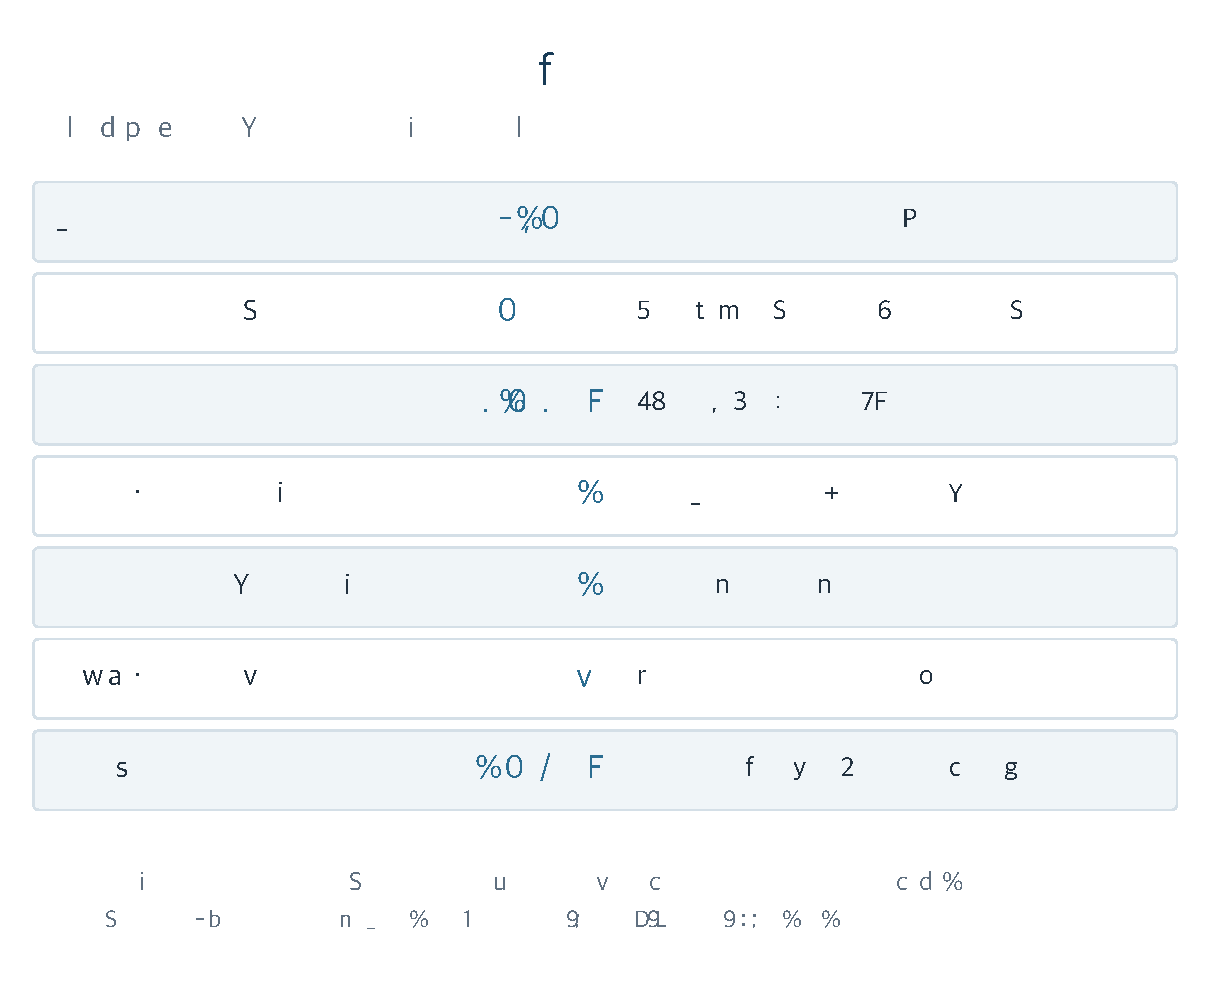
\includegraphics[width=0.90\textwidth]{docs/comprehensive_revision_20261026/figures/music_measurement_evidence_revised.pdf}
\caption{음악 보조지표의 측정대상별 비교}
\label{fig:music_econ_effective_burden}
\end{figure}

\begin{table}[H]
\centering
\caption{유튜브 결합상품과 개별 구매 조합의 표시가격 차이}
\label{tab:music_econ_bundle_subsidy}
\footnotesize
\setlength{\tabcolsep}{3.5pt}
\begin{tabular}{L{4.5cm}L{1.6cm}L{1.6cm}L{6.1cm}}
\toprule
\rowcolor{ReportTableHead}
비교 조합 & 가격차(원) & 비교대상 대비 & 해석 \\
\midrule
Lite + YouTube Music 개별 구매 & 5590 & 27.3\% & 두 상품을 따로 구매할 때보다 전체 Premium의 표시가격이 낮다. \\
Lite + 멜론 정가 상품 & 2290 & 13.3\% & Lite와 멜론을 함께 구매할 때보다 전체 Premium의 표시가격이 낮다. \\
암묵적 음악 가격 대 멜론 & 2290 & 26.4\% & Premium에서 Lite 가격을 뺀 잔여값을 멜론 정가와 비교한 산술값이다. \\
암묵적 음악 가격 대 Spotify & 5590 & 46.6\% & 같은 잔여값을 Spotify 개인 요금과 비교한 산술값이다. \\
Premium 대 Music 단독 & -2910 & -24.3\% & Premium에는 동영상 기능도 포함된다. 상품범위 차이를 함께 확인해야 한다. \\
\bottomrule
\end{tabular}

\vspace{0.3em}
{\par\raggedright\footnotesize 주: 기준은 2026년 3월 보존 가격이며, 가격차는 비교 조합에서 결합상품을 뺀 값이다. 암묵적 음악 가격 6,400원은 전체 Premium 14,900원에서 Lite 8,500원을 차감한 계산값이다. 이 잔여 가격이 소비자의 음악 가치평가, 회사의 음악 매출배분 또는 권리자 정산기초와 일치하는지는 별도 확인한다. 각 상품의 광고·오프라인·재생범위를 함께 비교해야 한다. 마지막 행의 음수는 Premium이 Music 단독보다 2,910원 비싸다는 뜻이다.\par}
\end{table}

\begin{figure}[H]
\centering
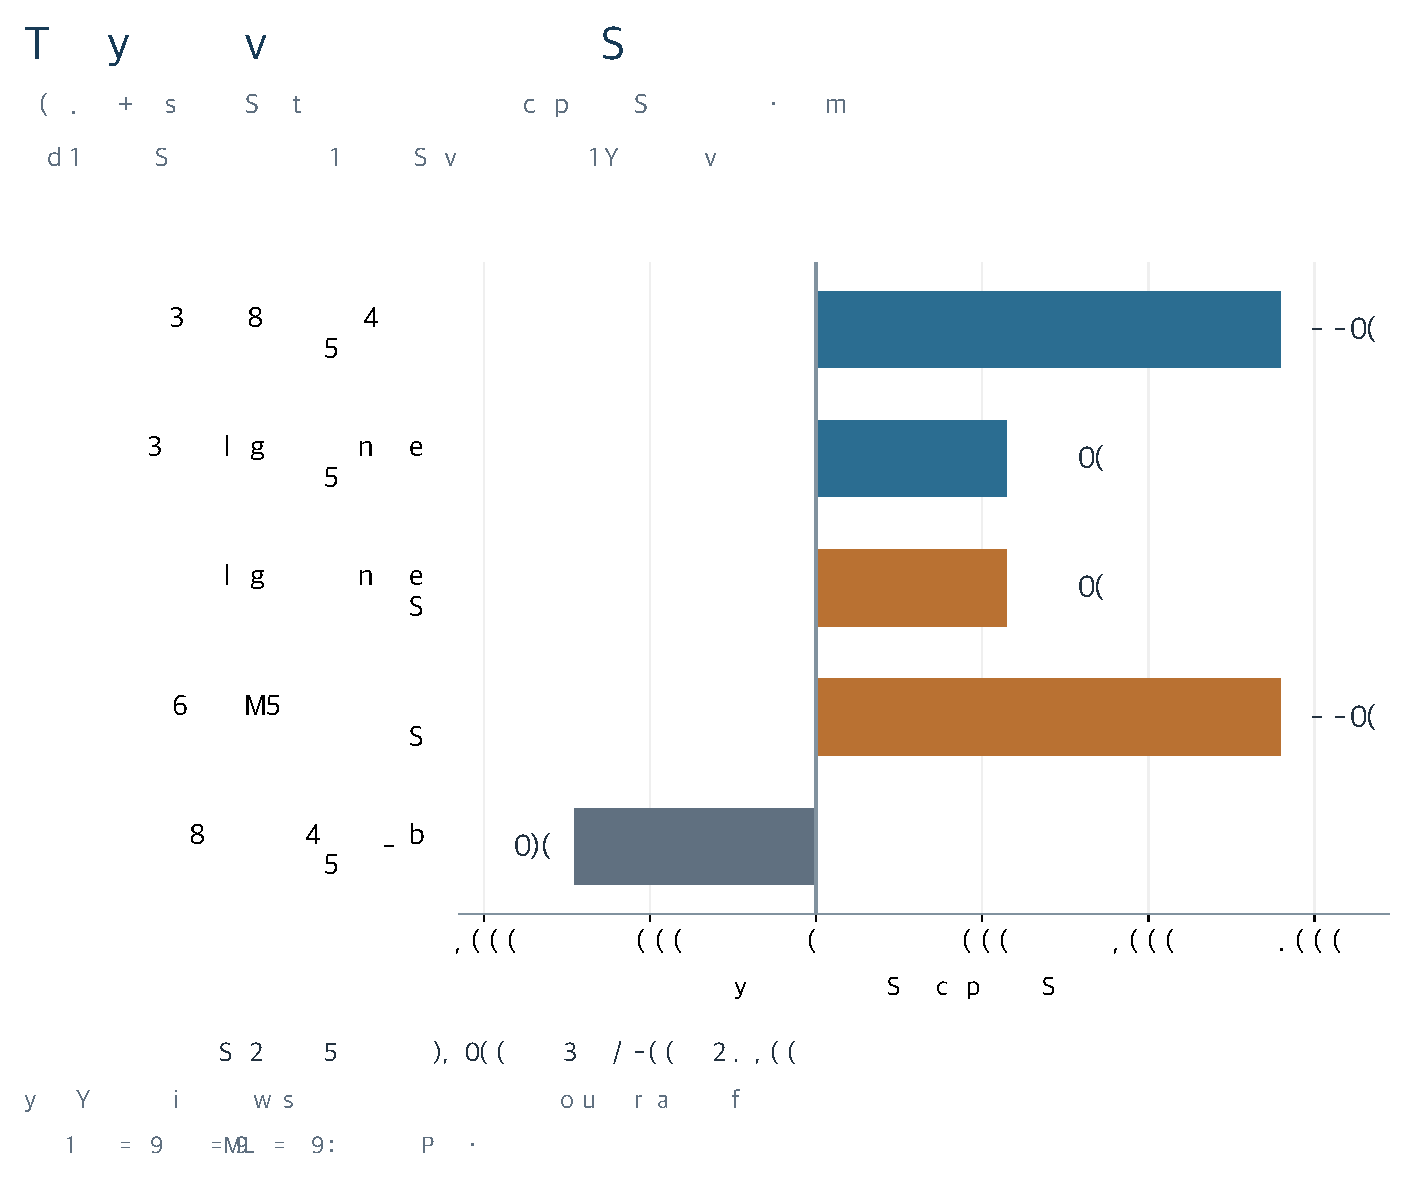
\includegraphics[width=0.90\textwidth]{docs/comprehensive_revision_20261026/figures/music_bundle_posted_price_comparison_revised.pdf}
\caption{유튜브 결합상품의 표시가격 조합 비교}
\label{fig:music_econ_bundle_subsidy}
\end{figure}

\begin{table}[H]
\centering
\caption{Premium Lite를 포함한 한국시장 유료 진입가격의 조건부 비교}
\label{tab:music_econ_premium_lite_did}
\footnotesize
\setlength{\tabcolsep}{4pt}
\begin{tabular}{L{4.3cm}rrrL{5.0cm}}
\toprule
\rowcolor{ReportTableHead}
비교 대상 & 가정 기준차 & 비교차 & 산술 변화 & 해석 \\
\midrule
YouTube 유료 진입 대 멜론 정가 & 3300 & -190 & -3490 & 가정한 기존 진입가격과 Lite 가격을 멜론 일반요금에 각각 대조한다. \\
YouTube 유료 진입 대 Spotify 개인 & 0 & -3490 & -3490 & Spotify Individual과 같은 가정 비교를 수행한 값이다. \\
\bottomrule
\end{tabular}

\vspace{0.3em}
{\par\raggedright\footnotesize 주: 단위: 원/월. 기존 YouTube Music 가격 11,990원을 가정한 유료 진입 기준점과 Lite 8,500원의 차이를 계산한 보정 비교다. 월별 출시 전 가격표와 출시 후 이용자·순위 패널은 확보되지 않았다. Lite는 대부분의 비음악 동영상용 상품이며 음원 단독상품과 기능이 다르다. 따라서 -3,490원은 상품구성 가정 아래의 산술 차이로, 멜론 이탈률이나 실제 음악가격 인하의 추정치로 사용하지 않는다.\par}
\end{table}

\begin{figure}[H]
\centering
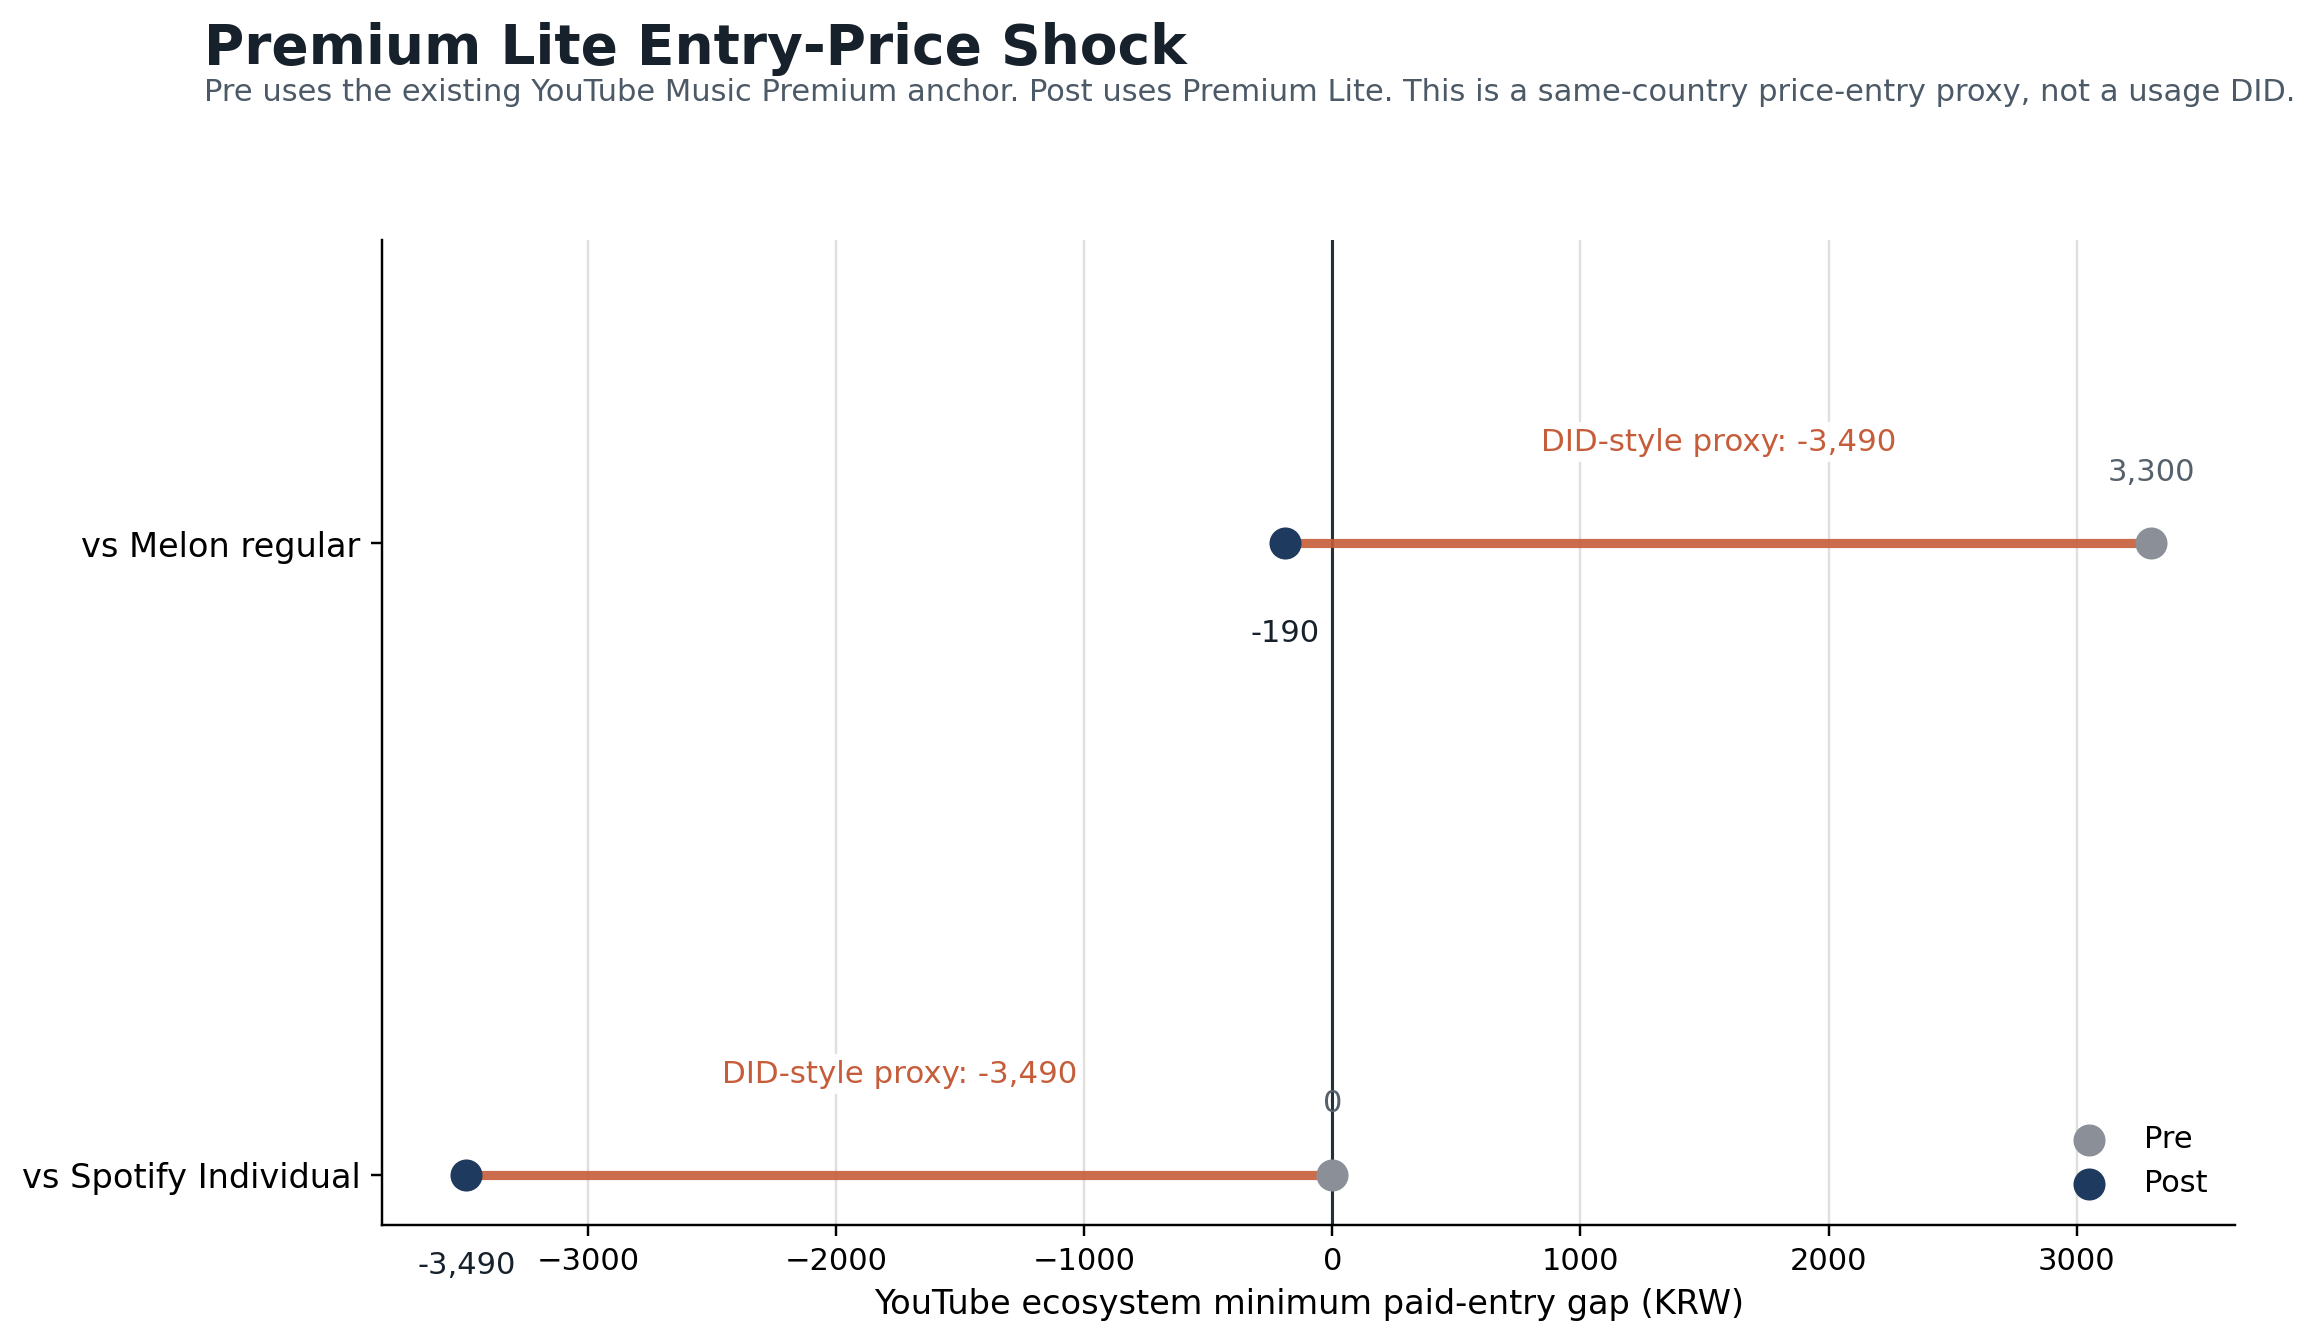
\includegraphics[width=0.90\textwidth]{outputs/figures/claim_strengthening/F_music_econ_premium_lite_entry_proxy.png}
\caption{Premium Lite를 포함한 유료 진입가격 비교 도식}
\label{fig:music_econ_premium_lite_entry}
\end{figure}

표~\ref{tab:claim_balanced_summary}에서 공통기간 균형 패널로 표본을 제한해도 세 비교 묶음의 격차 부호는 유지된다. 이 결과는 공통기간과 수준 비교 조건을 충족한 소수 관측치에 적용된다.

\begin{table}[H]
\centering
\caption{공통기간 균형 패널 재계산 요약}
\label{tab:claim_balanced_summary}
\small
\setlength{\tabcolsep}{4.5pt}
\begin{tabular}{L{3.5cm}rrrrr}
\toprule
\rowcolor{ReportTableHead}
비교 묶음 & 균형 패널 행수 & 국가 셀 수 & 재계산 격차 & 기존 격차 대비 변화 & 방향 유지 \\
\midrule
음악 스트리밍 & 3 & 1 & 16.592 & 0.000 & 예 \\
디지털 인프라 트래픽-OTT & 4 & 1 & -2.626 & 0.000 & 예 \\
음악 IP 수출 & 9 & 3 & -30.245 & 0.000 & 예 \\
\bottomrule
\end{tabular}

\vspace{0.3em}
{\par\raggedright\footnotesize 주: 균형 패널은 핵심 표본 중 공통기간과 수준 비교 조건을 모두 충족하는 관측치로 재계산했다. 격차의 방향은 유지되며 적용 범위는 해당 관측치에 한정된다.\par}
\end{table}

{\par\raggedright\footnotesize 근거: 표~\ref{tab:results_cpii_means}, 표~\ref{tab:claim_gap_main}, 표~\ref{tab:music_econ_effective_burden}, 표~\ref{tab:music_econ_bundle_subsidy}, 표~\ref{tab:music_econ_premium_lite_did}, 표~\ref{tab:claim_balanced_summary}, 그림~\ref{fig:claim_gap_main}, 그림~\ref{fig:music_econ_effective_burden}, 그림~\ref{fig:music_econ_bundle_subsidy}, 그림~\ref{fig:music_econ_premium_lite_entry}.\\
재현 산출물: \nolinkurl{T_claim_korea_vs_global_gap.csv}, \nolinkurl{T_claim_balanced_panel_summary.csv}, \nolinkurl{effective_burden_wedge_table.csv}, \nolinkurl{bundle_subsidy_wedge_table.csv}, \nolinkurl{premium_lite_did_results.csv}, \nolinkurl{F_music_econ_effective_burden_wedge.png}, \nolinkurl{F_music_econ_bundle_subsidy_ladder.png}, \nolinkurl{F_music_econ_premium_lite_entry_proxy.png}.\sourcefootnote{KCC 공식 자료, Cloudflare Radar(인증 수집 후보), OpenDART, SEC EDGAR, \srcYouTubeLite, \srcMelonPass, \srcSpotifyKR}\par}

한국시장 부담귀착 분석은 \texttt{reg-domestic}, \texttt{reach-gap}, \texttt{creator-incidence}, \texttt{market-transfer}를 구분한다. 멜론--유튜브 뮤직, 멜론--애플뮤직, FLO--스포티파이는 모두 국내 부담 방향으로 코딩되었다. 부담의 실제 규모와 원인을 비교하려면 국내외 서비스의 계약·원가자료를 대응시켜야 한다.

KOMCA는 별도의 유튜브 잔여사용료 청구시스템을 운영하며, 공식 FAQ는 대상 로그를 `2016Q3--2022Q2`의 한국 발생분으로 한정한다. 이는 해당 정산에 추가 청구·검증 절차가 존재한다는 근거다. 2025-05-22 보도들은 KOMCA가 의뢰한 EY한영 연구를 인용해 `10.5\% / 35\% / 83\%` 수익배분 구조와 `EY Analysis` 도표를 제시했다. 기사에서는 이를 `국내외 음악 스트리밍 시장 심층 분석 보고서` 또는 `음악 스트리밍 시장 보고서`로 부른다. 원 보고서 전문과 공식 다운로드 경로는 확보되지 않아, 해당 수치는 부록의 조건부 보조자료로 다룬다. 정산 절차의 존재와 보도된 배분률만으로 산업 평균 부담이나 개별 사업자의 부당 정산 여부를 판단할 수는 없다.

표~\ref{tab:claim_channel_decomp}와 그림~\ref{fig:claim_channel_decomp}는 기존 혼합 표본에서 국내 값과 비교군 값의 차이를 위험·시장 채널로 나누어 보여 준다. 디지털 인프라의 격차는 비용 및 회수위험 채널에서 발생하며, 음악 IP 수출은 시장 채널의 비중이 더 크다. 규제 채널은 활용 가능한 직접 비교자료가 부족하다. 음악의 주된 해석에는 동일시장 부담귀착 사례, 유튜브 결합상품 구조, 총매출 기준 정산, 창작자 보호비용 귀착을 사용한다.

표~\ref{tab:music_econ_channel_mediation}와 그림~\ref{fig:music_econ_channel_mediation}는 각 채널에 연결되는 관측자료를 정리한다. 제도·정산에는 라이선스 공개성 코딩과 조건부 정산 산술비교, 비용·위험에는 법인 회계상 유효세율과 거버넌스 증거항목, 시장·이용에는 결합상품 표시가격 차이와 앱 이용 규모를 배치했다. 이 구분에 따라 추가 수집할 계약·비용·이용 자료를 정할 수 있다.

\begin{table}[H]
\centering
\caption{국내·비교군 점수 차이의 채널별 비교}
\label{tab:claim_channel_decomp}
\footnotesize
\setlength{\tabcolsep}{3pt}
\begin{tabular}{L{3.3cm}rrrL{4.3cm}}
\toprule
\rowcolor{ReportTableHead}
비교 묶음 & 전체 격차 & 위험 채널 격차 & 시장 채널 격차 & 해석 \\
\midrule
음악 스트리밍 & 16.592 & 50.000 & 4.017 & 기존 혼합 표본의 비교값이며, 부담귀착 방향 사례와 비교 범위를 구분한다 \\
디지털 인프라 트래픽-OTT & -2.626 & -5.252 & 0.000 & 음의 전체 격차는 위험 채널에서 발생하며 시장 채널의 기여는 0 \\
음악 IP 수출 & -30.245 & -15.867 & -44.623 & 음의 전체 격차 중 절댓값 기준 약 73.8\%는 시장 채널에서 발생 \\
\bottomrule
\end{tabular}

\vspace{0.3em}
{\par\raggedright\footnotesize 주: 격차는 한국 값에서 비교군 값을 뺀 값이며, 음수는 해당 기존 점수에서 한국 값이 낮음을 뜻한다. 규제 채널은 현재 \texttt{no\_usable\_channel\_data} 상태라 본 표에 수치로 반영하지 않았다. 이 표는 위험·시장 채널에 한정한 기존 직접 비교다. 음악의 주된 해석에는 표~\ref{tab:signed_korea_market_case_studies}의 동일시장 사례, 유튜브 결합상품과 공개된 총매출 기준 정산규정을 사용한다.\par}
\end{table}

\begin{figure}[H]
\centering
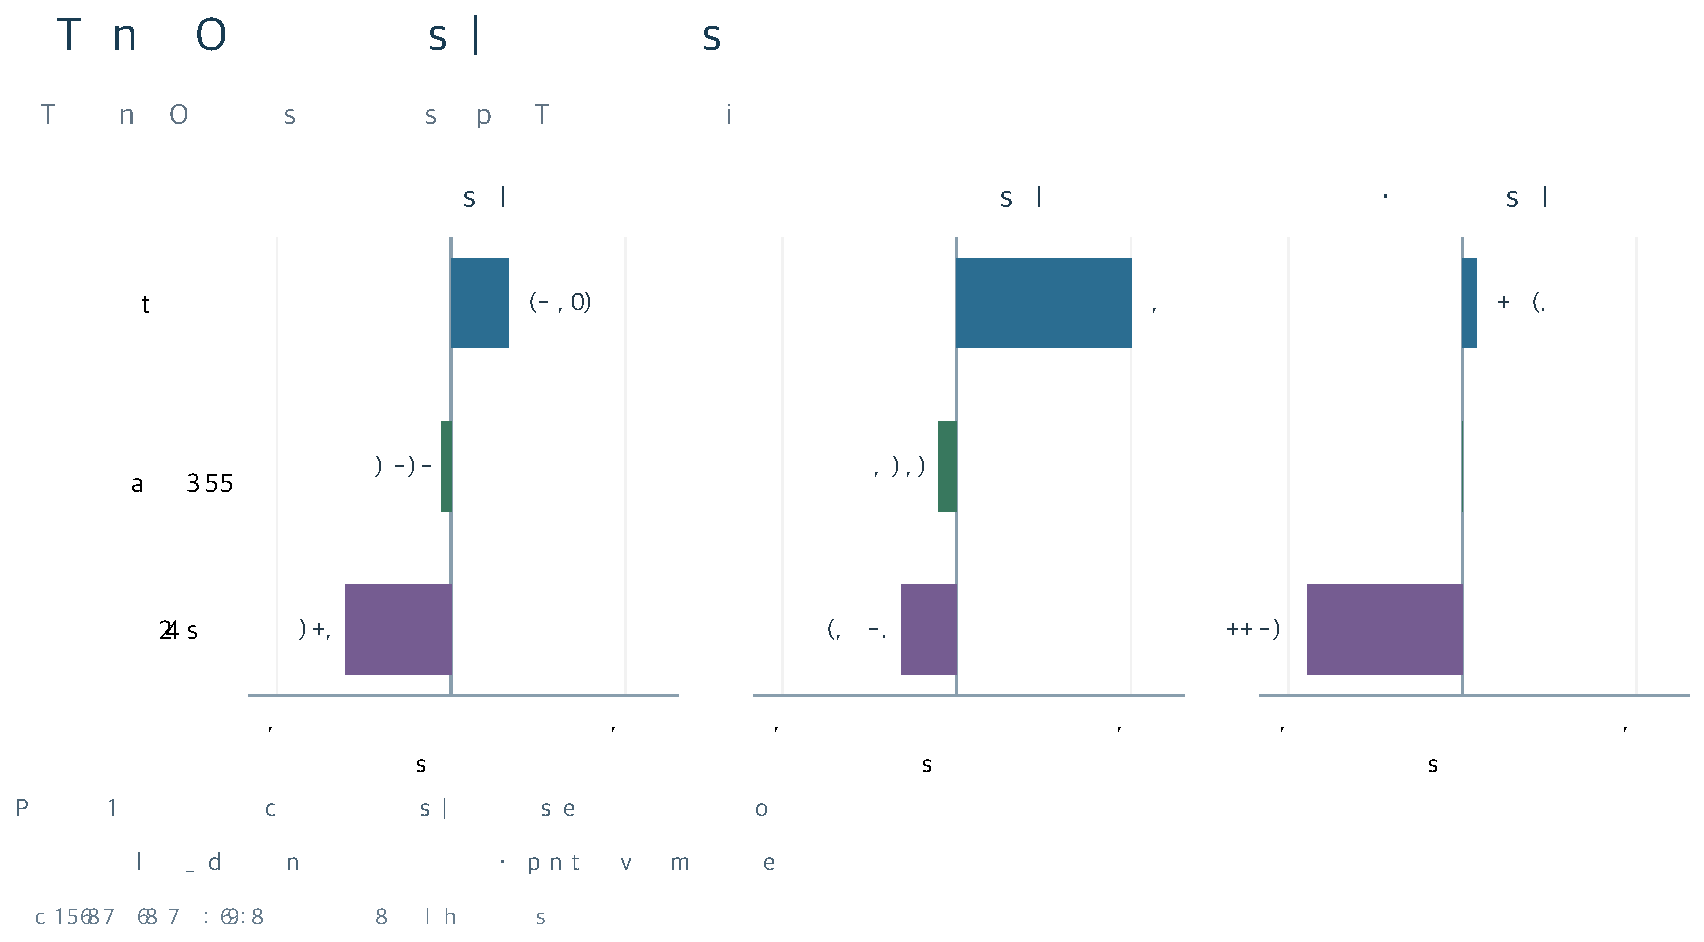
\includegraphics[width=0.88\textwidth]{docs/comprehensive_revision_20261026/figures/claim_channel_score_gaps_revised.pdf}
\caption{국내·비교군의 전체 점수와 채널별 점수 차이}
\label{fig:claim_channel_decomp}
\end{figure}

\begin{table}[H]
\centering
\caption{채널별 관측자료와 해석 범위}
\label{tab:music_econ_channel_mediation}
\footnotesize
\setlength{\tabcolsep}{3.5pt}
\begin{tabular}{L{2.2cm}L{2.3cm}L{1.4cm}L{6.8cm}}
\toprule
\rowcolor{ReportTableHead}
채널 & 보조지표 & 값 & 해석 \\
\midrule
제도·정산 & \WrapCell{라이선스 공개성\\코딩 차이} & 4 & 상품 공개 여부와 계약산식 공개 항목을 합산한 0--5 척도에서 국내 5와 해외 1의 차이. 실제 요율의 격차와 구분한다. \\
제도·정산 & \WrapCell{가격차/정산\\산술 기준값} & 2.510 & 2,290원을 $8,690\times0.105=912.45$원으로 나눈 조건부 비율이다. 실제 정산기초와 이용량 기준을 반영한 부담 한도는 별도 계산한다. \\
비용·위험 & \WrapCell{법인 회계상\\유효세율 차이} & 0.379 & FY2025 Dreamus와 Spotify의 회계상 유효세율 차이로, 한국 서비스 현금세부담과의 연결에는 추가 자료가 필요하다. \\
비용·위험 & \WrapCell{정산 거버넌스\\증거항목 순계} & 10 & 마찰 관련 12개 항목에서 완화 관련 2개 항목을 뺀 연구 코딩이다. 비용액을 측정한 값은 아니다. \\
시장·이용 & \WrapCell{동일시장\\결합상품 가격차} & 2290 & 전체 YouTube Premium의 표시가격이 Lite와 멜론의 개별 구매 합계보다 낮다. \\
시장·이용 & \WrapCell{동일월 이용\\비중 대리지표} & 0.135 & 2025년 5월 공통 관측에서 YouTube Music의 이용 비중 대리지표가 멜론보다 높다. \\
\bottomrule
\end{tabular}

\vspace{0.3em}
{\par\raggedright\footnotesize 주: 기존 채널과 보조 메커니즘의 연결표이다. 912.45원은 소비자 표시가격에 10.5\%를 곱한 기존 시나리오의 산술 기준값이다. 실제 정산에서는 매출액 정의, 관리비율, 광고·제휴 수익, 이용횟수·가입자수 방식과의 비교를 확인해야 한다. 따라서 2.510은 전체 사용료나 소비자 전가의 실증적 상한에 대한 비율로 해석하지 않는다.\par}
\end{table}

\begin{figure}[H]
\centering
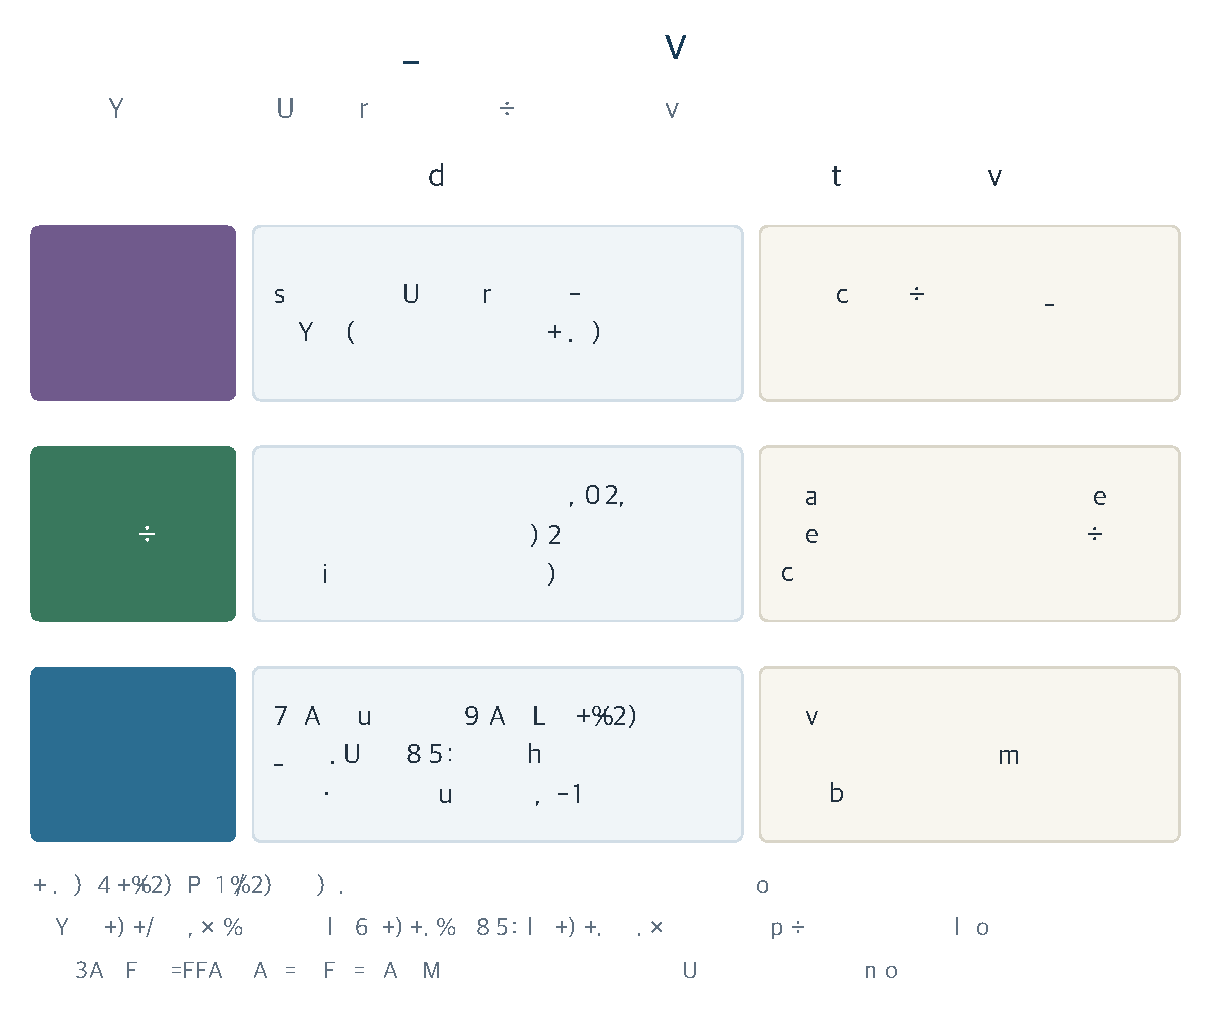
\includegraphics[width=0.92\textwidth]{docs/comprehensive_revision_20261026/figures/music_channel_evidence_map_revised.pdf}
\caption{음악 분야 채널별 관측과 추가자료}
\label{fig:music_econ_channel_mediation}
\end{figure}

{\par\raggedright\small 근거: 표~\ref{tab:claim_channel_decomp}, 그림~\ref{fig:claim_channel_decomp}, 표~\ref{tab:music_econ_channel_mediation}, 그림~\ref{fig:music_econ_channel_mediation}, \nolinkurl{T_claim_channel_decomposition.csv}, \nolinkurl{i_reg_narrow_panel.csv}, \nolinkurl{T_claim_leave_one_peer_out.csv}, \nolinkurl{econ_channel_mediation_table.csv}, \nolinkurl{F_music_econ_channel_mediation_map.png}. 출처: KCC 공식 자료, OpenDART, SEC EDGAR, \srcYouTubeLite, \srcMelonPass, \srcSpotifyKR, \srcKOMCAResidual, \srcChosunBizKOMCA, \srcBeyondPostKOMCA, \srcYonhapKOMCA, \srcAnewsKOMCA\par}



\section{웹툰 및 스토리 결과}
웹툰 및 스토리 분야에서도 서비스-분기 FE 패널의 직접효과는 유의하지 않았고, 서비스 기능 출시 사건을 사용한 stacked event study는 사전추세 검정이 실패했다. 표~\ref{tab:firm_case_studies}의 WEBTOON Entertainment·NAVER는 회사 수준 자료를, KakaoWebtoon·KakaoPage는 관측축이 제한된 방향 사례를 제공한다. 여기에 창작자 조사와 분야 평균을 연결해 회수위험과 정산구조를 살펴본다. 표~\ref{tab:results_webtoon_estimates}의 세부 추정치를 보면 사건 이후 계수보다 사건 이전 리드계수에서 더 강한 차이가 나타나므로, 현재 결과는 사건효과보다 사건 이전 이질성의 존재를 더 강하게 시사한다. 그러나 창작자 측 공식조사는 이 분야의 위험 채널을 별도로 보강한다. KOCCA의 2025 웹툰산업 실태조사에서 2024년 연재 경험이 있는 작가 866명의 연간 총소득 중위값은 3,700만 원, 평균 해외 소득 비중은 8.0\%, 해외 소득이 전혀 없는 응답은 43.8\%였다. 전체 작가 응답자 1,000명 기준으로 표준계약서 인지율은 66.0\%, 직접 불공정 계약·행위 경험 비율은 22.1\%였다. 수입 관련 문항과 계약 관련 문항의 응답자 범위를 구분하여 창작자 보호와 회수·정산구조를 함께 해석한다.\sourcefootnote{한국콘텐츠진흥원, \textit{2025 웹툰산업 실태조사}, 인쇄면 170쪽 표 2-29, 172쪽 본문·그림 2-17·표 2-31, 282쪽 표 2-137, 287쪽 표 2-142.}

\begin{table}[H]
\centering
\small
\caption{웹툰 및 스토리 분야 사건연구 및 강건성 추정치 요약표(T11-Webtoon)}
\label{tab:results_webtoon_estimates}
\begin{tabular}{llrrrrr}
\toprule
\rowcolor{ReportTableHead}
모형 & 설명변수 & N & 계수 & 표준오차 & $p$값 & 사전추세 \\
\midrule
FE panel & \texttt{foreign\_dependency\_ratio} & 39 & 28.659 & 108.893 & 0.792 & not applicable \\
Event study & \texttt{treated\_rel\_m1} & 170 & -68.795 & 18.642 & 0.000 & fail \\
Event study & \texttt{treated\_rel\_p1} & 170 & 8.533 & 18.286 & 0.641 & fail \\
Event study & \texttt{treated\_rel\_p2} & 170 & 10.884 & 23.172 & 0.639 & fail \\
\bottomrule
\end{tabular}
\end{table}

\begin{figure}[H]
\centering
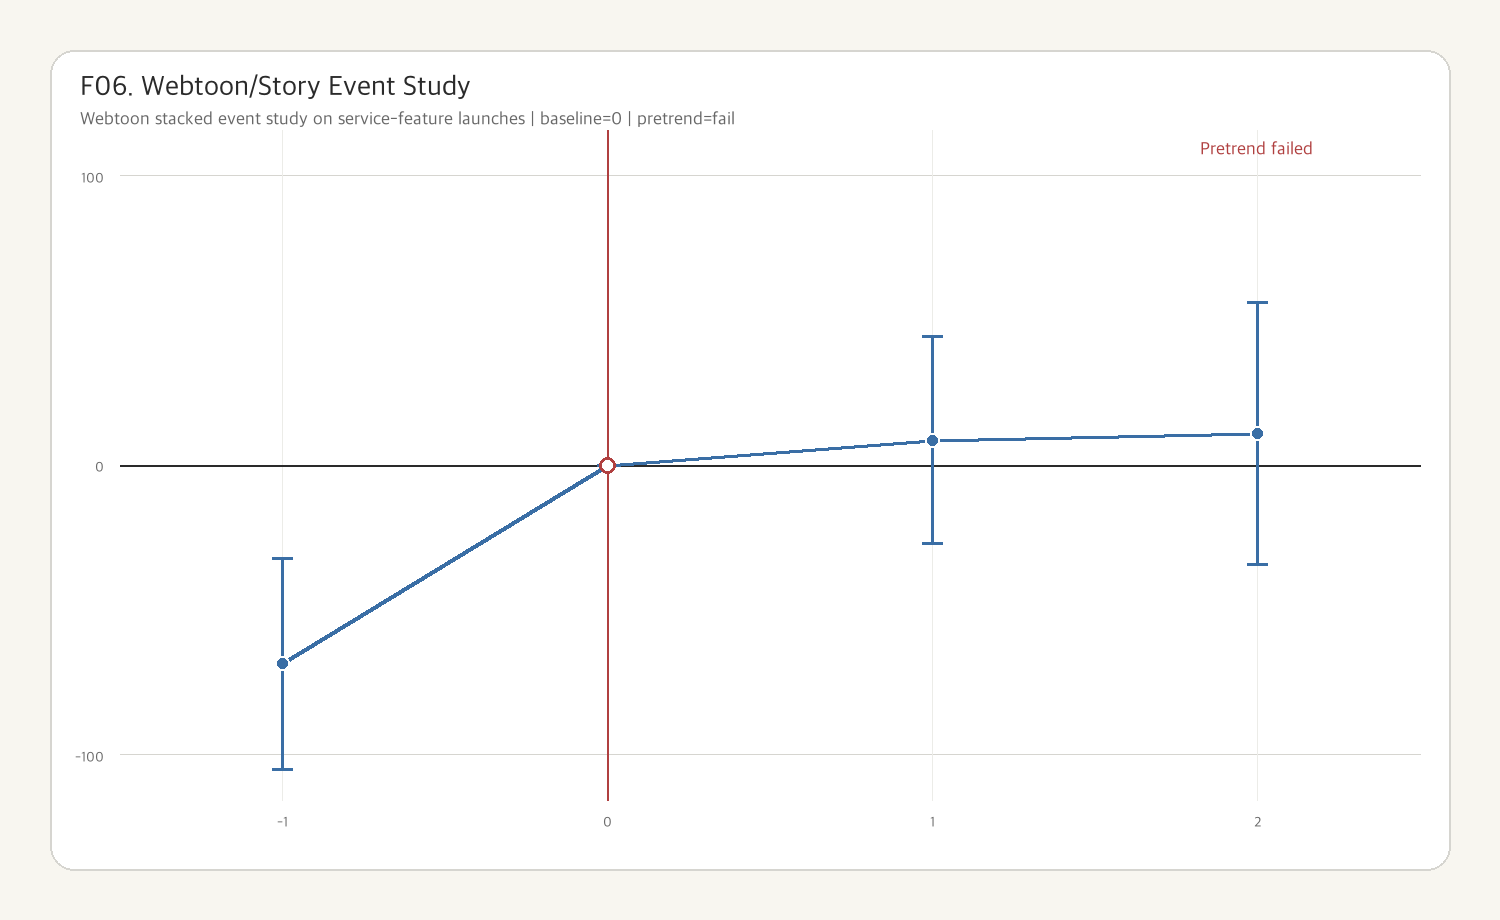
\includegraphics[width=0.92\textwidth]{outputs/figures/F06_webtoon_story_event_study_plot.png}
\caption{웹툰 및 스토리 분야 사건 전후 변화 그래프(F06)}
\label{fig:results_webtoon_event}
\end{figure}

웹툰 및 스토리의 전체 가용기간 평균 CPII는 54.23이다. 공통기간 3개 분기로 제한하면 음악과의 순위가 바뀌며, 분야-분기 점수는 2025Q4의 66.49와 2025Q2의 28.39 사이에 분포한다. 표~\ref{tab:firm_case_studies}의 WEBTOON Entertainment와 NAVER 자료, 작가 소득·계약 조사, 위험 하위지수는 회수위험과 정산구조를 이 분야의 우선 과제로 지목한다. 이 판단은 분야 서열보다 위험이 발생하는 경로와 분기별 변동에 초점을 둔다.

\section{디지털 인프라 결과}
디지털 인프라의 서비스-분기 회귀는 한국을 포함한 6개 시장의 자료를 사용한다. 해외의존 대리지표의 계수는 통계적으로 뚜렷하지 않았고, 망비용률과 비용/설비투자 비율 사이에는 양의 연관성이 나타났다. 두 비율이 같은 비용항을 공유하므로 이 계수에는 산술적 연결이 포함될 수 있다. 표~\ref{tab:results_infra_estimates} 하단의 국가 비교 회귀는 음악·웹툰·인프라를 합친 결과다. 제도·위험 하위지수와 시장 하위지수의 연관성을 보조적으로 보여 주며, 특정 분야의 정책효과는 별도 자료와 식별전략으로 확인해야 한다.

\begin{table}[H]
\centering
\small
\caption{인프라 6개 시장 회귀와 3분야 국가 비교 회귀(T11-Infra)}
\label{tab:results_infra_estimates}
\begin{tabular}{llrrrrr}
\toprule
\rowcolor{ReportTableHead}
표본 & 설명변수 & N & 계수 & 표준오차 & $p$값 & 사전추세 \\
\midrule
6개 시장 FE & \texttt{foreign\_dependency\_ratio} & 108 & 1.144 & 2.287 & 0.617 & not applicable \\
6개 시장 FE & \texttt{network\_cost\_ratio} & 108 & 126.118 & 23.422 & 0.000 & not applicable \\
3분야 국가 비교 & \texttt{I\_reg} $\rightarrow$ \texttt{I\_market} & 64 & 0.463 & 0.094 & 0.000 & not applicable \\
3분야 국가 비교 & \texttt{I\_risk} $\rightarrow$ \texttt{I\_market} & 64 & -1.976 & 0.284 & 0.000 & not applicable \\
\bottomrule
\end{tabular}
\end{table}

\begin{figure}[H]
\centering
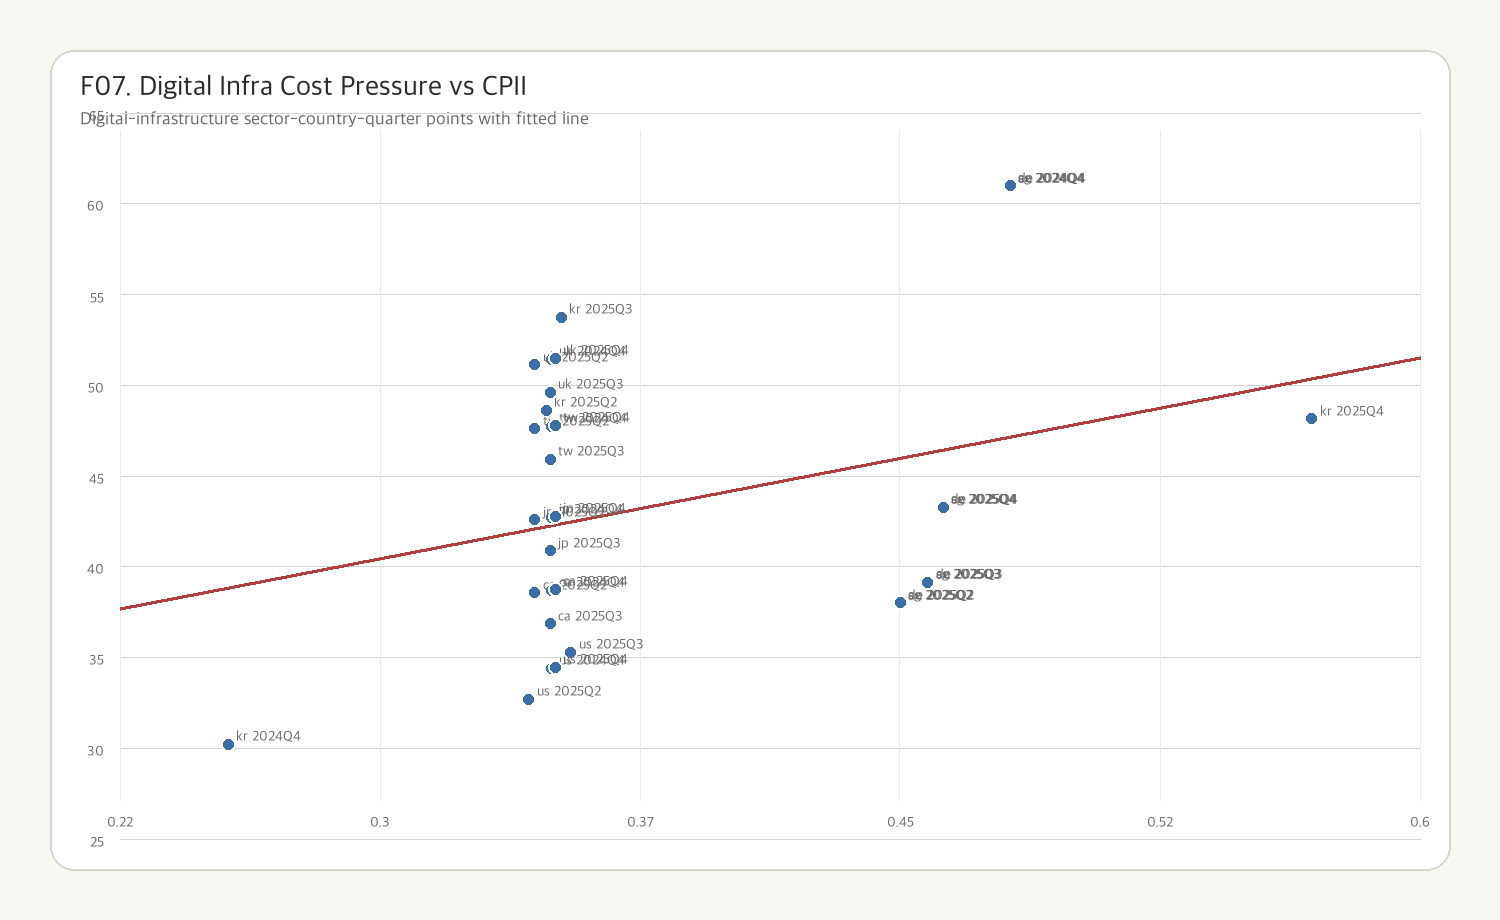
\includegraphics[width=0.92\textwidth]{outputs/figures/F07_digital_infra_pressure_scatter.png}
\caption{디지털 인프라 비용압력-불평등 관계 그래프(F07)}
\label{fig:results_infra_scatter}
\end{figure}

수준 비교에서는 디지털 인프라의 평균 CPII가 43.00으로 세 분야 중 가장 낮았지만, 국가 및 기업 간 격차는 여전히 컸다. 분야-분기 기준 범위는 2024Q4의 41.79에서 2025Q4의 43.92까지였고, FY2024 annual 추가 확보와 영국·대만 2024Q4 공식 국가 proxy 보강으로 한국 통신 3사와 해외 비교군 \texttt{akamai}, \texttt{alphabet}, \texttt{amazon}, \texttt{cloudflare}, \texttt{netflix}가 모두 2024Q4--2025Q4의 4개 공통 비교 구간을 확보했다는 점이 특히 중요하다. Twitch는 공식 철수 공지에서 한국 네트워크 비용이 ``대부분의 다른 국가보다 약 10배'' 높았다고 밝혔다. 이는 해당 기업이 제시한 비용압력의 공개 사례다. 표~\ref{tab:firm_case_studies}에서 보듯, KT의 직접 비교근거와 SK Telecom·LG Uplus의 부호가 혼합된 근거는 회사 평균과 한국 관련 부호형 사례점수를 각각 분리해 읽은 결과다.

\subsection{실행 회귀의 표본과 불확실성}
표~\ref{tab:results_infra_estimates}의 인프라 회귀는 6개 시장에서 관측한 서비스-분기 108행을 사용한다. 한국 8행과 영국·미국·일본·대만·캐나다 각 20행이며, 서로 다른 기업-분기 조합은 23개다. 한국 통신 3사의 완전관측 회귀행은 각각 2025Q4 한 행이다. 회사 평균 CPII에 사용한 4개 분기와 회귀에 필요한 모든 변수가 동시에 관측된 분기는 구별된다. 이 표의 국가 비교 보조회귀는 음악 24행, 웹툰 및 스토리 19행, 인프라 21행을 합친 64행으로 추정한다. 따라서 국가 비교 계수는 세 분야를 합친 연관성이다.

실행 코드는 인프라 회귀에 서비스와 분기 고정효과를, 국가 비교 회귀에 분야와 분기 고정효과를 포함한다. 표준오차는 행별 이분산성을 허용하는 HC1 방식이며, 보고된 $p$값은 정규분포 근사를 사용한다. 기업별 또는 국가별 군집 상관, 공시 이월값과 여러 시장에 반복 연결된 동일 재무자료의 상관은 이 표준오차에 반영되지 않는다. 따라서 유의성은 저장된 실행 사양의 계산 결과로 해석하며, 독립적인 기업별 변화와 군집 단위의 불확실성은 후속 추정에서 점검해야 한다.

비율의 공유 원자료도 해석에 영향을 준다. 망비용률과 설비투자 압박률에는 동일한 망·클라우드 비용이 분자로 들어간다. 이 때문에 두 비율 사이의 양의 회귀계수에는 공통 비용항의 산술적 연결이 포함될 수 있다. 비용 원자료, 매출 및 설비투자를 분리한 회귀와 기업 단위 반복관측 처리를 추가하면 경제적 전달경로의 범위를 더 구체화할 수 있다. 근거: \nolinkurl{scripts/run_sector_regressions.py}, \nolinkurl{docs/comprehensive_revision_20261026/project_gap_quant_checks.json}.


\section{정책 시나리오 결과}
기존 산출물은 기준 시나리오 44개와 민감도 관측치 132개다. NET의 기존 평균 변화량은 \(+8.575\)점으로 가장 크다. BND, IPF, CBA는 각각 \(-0.505,-1.583,-1.342\)점이다. 이 변화량에는 정책충격 외에 기존 분야 평균과 시나리오 입력 재구성 사이의 차이가 섞여 있으므로, 음수만으로 정책 악화를 판정하지 않는다. 기존 수치를 보존하면서 무변경 재계산과 공통 셀 비교로 그 차이를 분리한다.

\begin{table}[H]
\centering
\small
\caption{정책 시나리오 기존 산출값과 민감도 범위(T12)}
\label{tab:results_policy_scenarios}
\begin{tabular}{lrrrrrr}
\toprule
\rowcolor{ReportTableHead}
시나리오 & 평균 $\Delta \mathrm{CPII}$ & 최소 & 최대 & 최신 우선순위 & 최신 점수 & 해석 \\
\midrule
NET & 8.575 & -1.884 & 20.052 & 1 & 0.1000 & 기존 평균 최대 \\
BND & -0.505 & -8.934 & 4.279 & 2 & 0.0334 & 기준값 분리 필요 \\
IPF & -1.583 & -12.956 & 3.633 & 3 & 0.0184 & 기준값 분리 필요 \\
CBA & -1.342 & -13.872 & 4.545 & 4 & 0.0078 & 기준값 분리 필요 \\
\bottomrule
\end{tabular}
\end{table}

전체 평균표는 1차 선별 용도다. 실제 정책판단은 적어도 세 층위로 읽어야 한다. 첫째, 시나리오별 전체 평균 $\Delta \mathrm{CPII}$로 전반적 방향을 확인한다. 둘째, 분야별 표로 어느 시장에서 효과가 반복되는지 확인한다. 셋째, 해당 시나리오가 $I^{\mathrm{reg}}$, $I^{\mathrm{risk}}$, $I^{\mathrm{market}}$ 중 어느 채널을 주로 움직이는지 확인해야 한다. 따라서 표~\ref{tab:results_policy_scenarios}만으로 최종 권고를 정하는 것은 충분하지 않다.

\begin{table}[H]
\centering
\small
\caption{분야별 정책 시나리오 결과}
\label{tab:results_policy_by_sector}
\begin{tabular}{L{2.5cm}L{1.2cm}rrrrr}
\toprule
\rowcolor{ReportTableHead}
분야 & 시나리오 & 가용 분기 수 & 평균 $\Delta \mathrm{CPII}$ & 최신분기 & 최신 $\Delta \mathrm{CPII}$ & 최신 순위 \\
\midrule
음악 & \texttt{BND} & 6 & -1.238 & 2026Q1 & -8.934 & 1 \\
음악 & \texttt{NET} & 6 & 8.070 & 2026Q1 & 3.054 & 2 \\
음악 & \texttt{IPF} & 6 & -2.988 & 2026Q1 & -8.018 & 3 \\
음악 & \texttt{CBA} & 6 & -2.678 & 2026Q1 & -8.934 & 4 \\
\midrule
웹툰 및 스토리 & \texttt{BND} & 4 & 0.595 & 2026Q1 & -2.068 & 2 \\
웹툰 및 스토리 & \texttt{NET} & 4 & 13.800 & 2026Q1 & 15.477 & 1 \\
웹툰 및 스토리 & \texttt{IPF} & 4 & 0.525 & 2026Q1 & -2.068 & 3 \\
웹툰 및 스토리 & \texttt{CBA} & 4 & 0.661 & 2026Q1 & -2.068 & 4 \\
\midrule
디지털 인프라 & \texttt{NET} & 4 & 4.107 & 2025Q4 & 6.605 & 1 \\
\bottomrule
\end{tabular}
\end{table}

\noindent{\footnotesize 주: 디지털 인프라는 설계상 \texttt{NET}만 계산 가능하여 다른 시나리오는 제외했다. 최신분기는 음악과 웹툰 및 스토리가 2026Q1, 디지털 인프라가 2025Q4다. `최신 순위`는 해당 분야 최신분기의 \texttt{policy\_priority\_score} 기준 순위이므로 최신 $\Delta \mathrm{CPII}$의 단순 크기순과 일치하지 않을 수 있다.}

\begin{figure}[H]
\centering
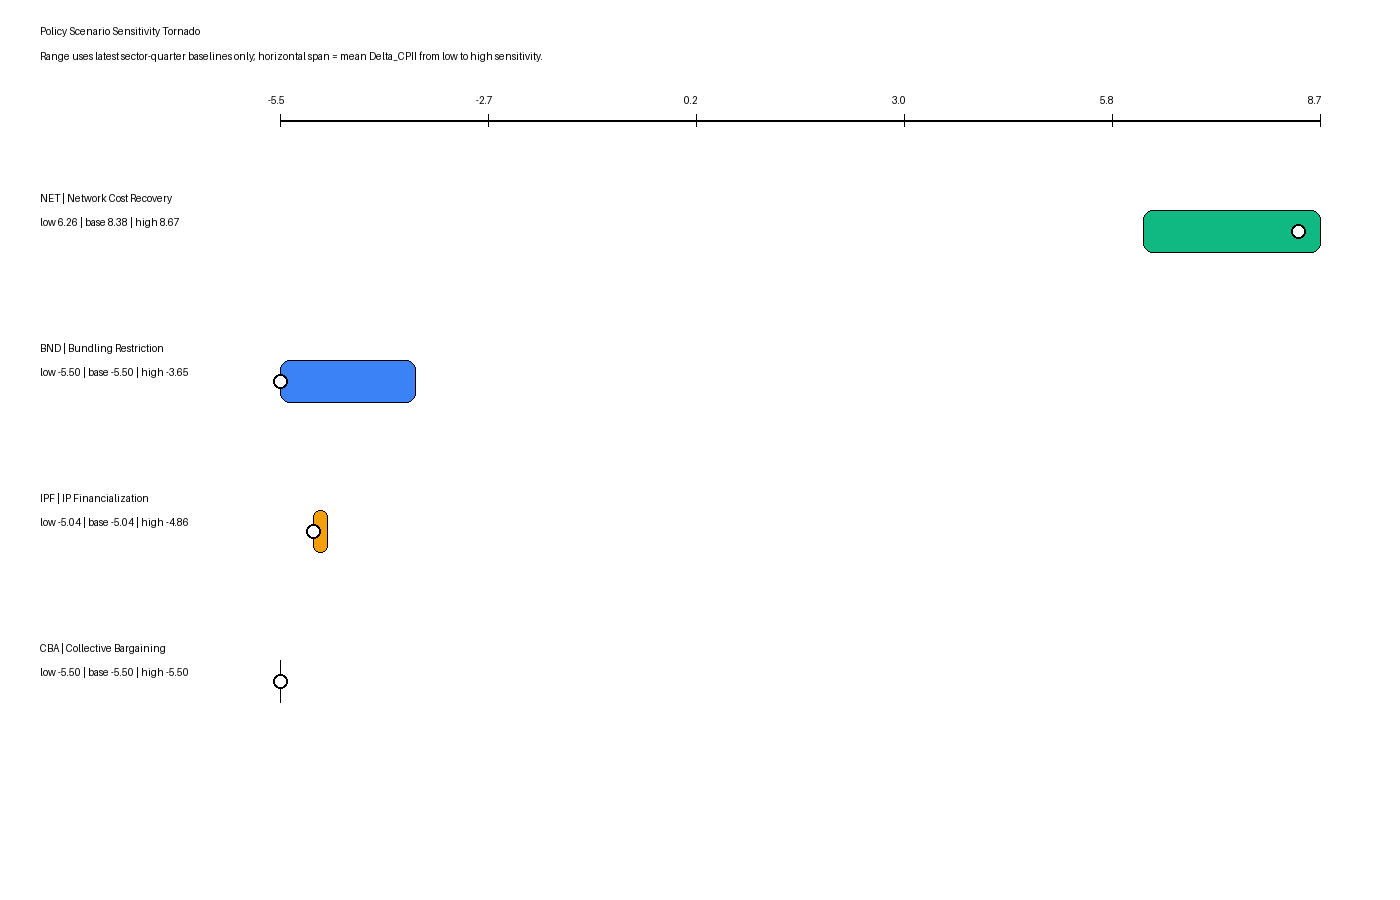
\includegraphics[width=0.92\textwidth]{outputs/figures/policy_tornado_chart.png}
\caption{정책 시나리오 민감도 차트(F10)}
\label{fig:results_policy_sensitivity}
\end{figure}

기존 시나리오 점수 차이는 분야별로 달랐으며 기준값 재구성 차이를 포함한다. 웹툰 및 스토리 분야에서는 \texttt{NET}이 2025Q4에 $+20.05$, 2026Q1에 $+15.48$의 기존 점수 차이를 보였다. 디지털 인프라는 설계상 \texttt{NET}만 계산 가능했고, 최신분기인 2025Q4에서 개선폭은 $+6.60$이었다. 반면 음악 분야의 최신분기 2026Q1에서는 \texttt{NET}이 $+3.05$에 그쳤고 2025Q4에는 오히려 $-1.88$를 기록해, \texttt{BND}, \texttt{IPF}, \texttt{CBA}와 함께 분야별 추가 보정 필요성을 시사했다. 따라서 이 수치는 다음 절의 기준값 재구성 분해와 같은 셀의 정책 간 차이를 함께 읽어야 한다. 정책표의 전체 평균은 요약값이고, 실제 권고는 표~\ref{tab:results_policy_by_sector}와 각 시나리오의 채널별 목표 하위지수를 결합해 내려야 한다.

\noindent{\small 근거: 표~\ref{tab:results_policy_scenarios}, 그림~\ref{fig:results_policy_sensitivity}.}\sourcefootnote{KOCCA 조사자료, KCC 공식 자료, OpenDART, SEC EDGAR, Cloudflare Radar(인증 수집 후보)}

\subsection{기준값과 시나리오 변화의 분리}
기존 분야 CPII는 국가별 하위지수를 평균한 값이다. 반면 시나리오는 분야별 중앙값, 보정 입력, 결측 보완값으로 재구성한 벡터에 고정 기준점을 적용한다. 일부 과거 분기에는 후속 분기 값을 소급 대입한다. 비선형 순위변환과 집계 순서도 달라, 무변경 입력을 다시 계산한 점수조차 기존 CPII와 일치하지 않는다.
\[
\begin{aligned}
\mathrm{CPII}^{(0)}_{s,q}
&=\mathcal A\!\left(\{\mathcal N_{j,\mathrm{base}}
(z^{\mathrm{base}}_{j,s,q})\}_{j\in\mathcal J}\right),\\
b^{\mathrm{rebase}}_{s,q}
&=\mathrm{CPII}^{\mathrm{base}}_{s,q}-\mathrm{CPII}^{(0)}_{s,q},\\
D^{(p)}_{s,q}
&=\mathrm{CPII}^{(0)}_{s,q}-\mathrm{CPII}^{(p)}_{s,q},\\
\Delta\mathrm{CPII}^{(p)}_{s,q}
&=b^{\mathrm{rebase}}_{s,q}+D^{(p)}_{s,q}.
\end{aligned}
\]
\(b^{\mathrm{rebase}}\)는 기준값 재구성 차이, \(D^{(p)}\)는 같은 재구성 입력에 시나리오를 적용한 기계적 점수 차이다. 위첨자 \((0)\)은 입력을 그대로 둔 재계산이며, 경계값 처리가 포함된 시나리오 함수에 정책강도 0을 넣는 것과도 다를 수 있다.

예를 들어 웹툰 2026Q1은 기존 CPII 65.640, 무변경 재계산값 67.708이다. BND 적용값도 67.708이므로 기존 변화량 -2.068점은 전부 기준값 차이다. 이를 번들 압력 축소가 불평등을 악화시켰다는 결과로 읽을 수 없다. 이하 기존 수치는 보존하고, 표~\ref{tab:policy_decomposition}에서 기준값 차이를 별도 분해한다.

\subsection{시나리오 경계값과 측정 일관성}
BND의 로컬 점유율은 매출 회복액 계산에만 사용되며, 활성 CPII 입력은 시장전이 변수다. NET은 망비용률과 해외의존도를 바꾸면서 그 곱으로 정의된 인프라 의존 변수는 고정한다. 설비투자 대비 비용비율에서 매출 대비 투자증분을 차감하는 식도 회계항등식이 아니라 전달 가정이다.

IPF는 조달스프레드에 0 하한을 적용하므로, 음수인 기준 스프레드는 정책강도가 0이어도 0으로 상승한다. 음악의 두 기준분기에서는 이 처리만으로 재계산 CPII가 각각 1.901점 상승한다. 음수인 IP 격차에 \(1-\alpha^{\mathrm{ip}}\)를 곱할 때도 격차가 상승한다. 이를 금융 자산화의 악화효과와 구별해야 한다.

CBA는 창작자 배분률에 1의 상한을 두면서 소득증분과 회수율에는 상한 전 증분을 사용한다. 웹툰의 네 기준분기에서 이 문제가 발생한다. 기준 배분률 \(R^{\mathrm{cr}}\), 가정한 증분 \(\Delta R^{\mathrm{cr}}\), 적용대상 매출 \(E\)에 대해 유효 증분과 일관된 소득증분은
\[
\delta^{\mathrm{eff}}=\min\{1,R^{\mathrm{cr}}+\Delta R^{\mathrm{cr}}\}-R^{\mathrm{cr}},
\qquad \mathrm{CreatorIncomeGain}^{*}=E\delta^{\mathrm{eff}}
\]
다. 회수율에도 같은 유효 증분을 사용해야 한다. 기존 CBA 소득증분과 우선순위는 이 수정 전 가정값이며 실현가능한 증가액으로 해석하지 않는다.

이 차이들은 보정된 입력에 대한 민감도 비교와 독립된 정책효과 추정을 구별하게 한다. 정책 입력 일부는 기존 하위지수로부터 보정되어 있어, 지수와 독립된 새로운 경제적 관측치도 아니다. 비용·회수율의 실제 개선은 가격, 계약, 투자 및 정산 자료로 별도 확인해야 한다.

\begin{table}[H]
\centering
\small
\caption{정책 변화량의 분야별 분해: 동일 재구성 입력 기준}
\label{tab:policy_decomposition}
\begin{tabular}{@{}L{2.4cm}lrrrr@{}}
\toprule
\rowcolor{ReportTableHead}
분야 & 시나리오 & 평균 \(\Delta\mathrm{CPII}\) & 평균 \(b^{\mathrm{rebase}}\) & 평균 \(D^{(p)}\) & 최신 \(D^{(p)}\)\\
\midrule
음악 & BND & -1.238 & -2.781 & 1.543 & 0.000\\
음악 & NET & 8.070 & -2.781 & 10.851 & 11.988\\
음악 & IPF & -2.988 & -2.781 & -0.207 & 0.916\\
음악 & CBA & -2.678 & -2.781 & 0.103 & 0.000\\
\midrule
웹툰 및 스토리 & BND & 0.595 & 0.595 & 0.000 & 0.000\\
웹툰 및 스토리 & NET & 13.800 & 0.595 & 13.205 & 17.545\\
웹툰 및 스토리 & IPF & 0.525 & 0.595 & -0.070 & 0.000\\
웹툰 및 스토리 & CBA & 0.661 & 0.595 & 0.066 & 0.000\\
\midrule
디지털 인프라 & NET & 4.107 & -3.771 & 7.877 & 9.661\\
\bottomrule
\end{tabular}
\par\smallskip
\begin{minipage}{\linewidth}
\footnotesize\raggedright 주: 같은 보정 입력과 고정 정규화 기준점을 사용한 무변경 재계산과의 비교. 반올림 전 \(\Delta\mathrm{CPII}=b^{\mathrm{rebase}}+D^{(p)}\) 성립. \(D^{(p)}\)에도 시나리오 하한·상한 및 대체값 처리의 영향 포함. 순수 정책효과의 추정치나 신뢰구간 아님. 최신분기는 음악·웹툰 2026Q1, 인프라 2025Q4.
\end{minipage}
\end{table}

전체 평균에서 NET은 14개 분야-분기, 나머지 시나리오는 음악·웹툰의 10개 분야-분기를 사용한다. 따라서 분야 구성이 다른 평균의 순위만으로 정책을 선택할 수 없다. 민감도 표의 최소·최대는 전달계수를 기준의 0.8배·1.0배·1.2배로 조정하고 사전 허용범위로 제한한 계산값들의 범위이며, 표본오차에 대한 신뢰구간은 아니다.

기존 우선순위 점수 \(\Pi\)는 다음 임의 가중합이다. 아래첨자와 시나리오 위첨자는 생략한다.
\[
\begin{aligned}
\Pi={}&0.55\frac{(\Delta\mathrm{CPII})_+}{\max(\mathrm{CPII}^{\mathrm{base}},1)}
+0.15\frac{(RR)_+}{\max(M,1)}
+0.10\frac{(DC)_+}{\max(R,1)}\\
&+0.10\frac{(NG)_+}{\max(C^{\mathrm{IPF}},1)}
+0.10\frac{(CG)_+}{\max(E,1)} .
\end{aligned}
\]
\(RR,DC,NG,CG\)는 각각 매출 회복액, 국내 설비투자 증가액, 추가 순현재가치, 창작자 소득증분이다. 해당 시나리오에서 계산하지 않는 증분은 0이다. \(M,R,C^{\mathrm{IPF}},E\)는 각각 시장매출, 기준매출, 콘텐츠 투자액, 적용대상 매출이며 금액 단위는 원이다. \((u)_+=\max(u,0)\)이므로 CPII 악화분은 점수에서 벌점으로 반영되지 않는다. 음악 BND가 음의 기존 변화량에도 최신 1위인 이유는 매출 회복 가정이 별도로 가산되기 때문이다. 이 점수는 사회후생 함수가 아니며, CBA 상한 문제도 포함한다.

최신 종합점수는 각 분야의 마지막 가용 분기에서 계산한 \(\Pi\)를 시나리오별로 동일가중 평균한 값이다. NET은 세 분야, 나머지는 음악·웹툰 두 분야를 포함하므로 분야 구성도 다르다.

\section{부담 방향과 정책 비교의 강건성}
\subsection{단일 축과 가중치 의존성}
부담귀착 방향의 반복성이 특정 축 하나나 동일가중 선택에만 의존하는지 확인한다. 비교행 \(r\)의 관측 확장축 집합을 \(O_r\)로 두고, 축 \(h\)를 제외한 평균과 가중평균의 최솟값을 계산한다.
\[
S^{(-h)}_r=\frac{\sum_{k\in O_r\setminus\{h\}}a_{r,k}}{|O_r|-1},
\qquad
S^{\min}_r=
\min_{\{w_k\in[0.5,2]\}_{k\in O_r}}
\frac{\sum_{k\in O_r}w_k a_{r,k}}{\sum_{k\in O_r}w_k}.
\]
첫 식은 관측축이 두 개 이상일 때 계산한다. 두 번째 식은 축 간 가중치 비율을 최대 4배까지 허용한 가장 불리한 조합이다. 고정된 다른 가중치 아래에서 목적함수는 각 가중치에 대해 단조이거나 일정하므로, 모든 가중치를 0.5 또는 2로 둔 꼭짓점을 열거하면 최솟값을 얻는다.

\begin{table}[H]
\centering
\small
\caption{확장 부담귀착 방향점수의 축 제외·가중치 민감도}
\begin{tabular}{@{}L{2.5cm}rrrr@{}}
\toprule
\rowcolor{ReportTableHead}
분야 & 사례 수 & 축 1개 제외 최저점 & 가중치 변경 최저점 & 핵심축 제외 양수 유지\\
\midrule
음악 & 6 & 0.283 & 0.300 & 6/6\\
웹툰 및 스토리 & 2 & 0.125 & 0.117 & 계산 불가\\
디지털 인프라 & 3 & 0.228 & 0.054 & 1/3\\
\bottomrule
\end{tabular}
\par\smallskip
\begin{minipage}{\linewidth}
\footnotesize\raggedright 주: 두 최저점은 각 분야의 모든 사례·허용 조합 중 최솟값. 마지막 열은 별도로 핵심 점수에서 관측축을 하나씩 제외해도 항상 양수인 사례 수. 웹툰 핵심축은 사례당 1개여서 제외 후 점수 산출 불가.
\end{minipage}
\end{table}

\textbf{관측된 11개 확장 사례 모두에서 단일 축을 제외하거나 가중치 비율을 4배까지 바꾸어도 국내 부담 방향이 유지된다.} 음악은 핵심 점수에서도 6개 사례 모두 같은 성질을 보인다. 따라서 음악의 반복 관측은 확장축 추가나 특정 단일 축만의 결과가 아니다. 인프라는 KT만 핵심축 제외에도 양수를 유지하며, SK Telecom·LG Uplus의 위험-회수 축은 각각 음수다. 규제와 규제 포착범위를 동시에 제외하면 이 두 사례의 부호는 음수로 바뀐다. 웹툰은 확장 방향은 안정적이지만 핵심축의 추가 관측이 필요하다. 이 분석은 주어진 사례와 축 점수에 대한 결정론적 민감도 점검이며, 독립 표본의 통계적 유의성이나 자료 코딩의 정확성을 검정한 결과는 아니다.

분야별 채널 차이도 기간 평균만의 현상인지 확인했다. 웹툰은 가용 4개 분기 모두 \(I^{\mathrm{risk}}>I^{\mathrm{market}}\), 인프라는 4개 분기 모두 위험 하위지수가 다른 두 하위지수보다 높았다. 음악은 6개 중 5개 분기에서 \(I^{\mathrm{market}}>I^{\mathrm{risk}}\)였다. 평균 총점보다 \textbf{음악의 시장전이·의존 구조, 웹툰과 인프라의 회수위험 구조를 분리하는 접근}이 반복 관측에 더 잘 부합한다.

\subsection{같은 분야·분기의 정책 비교}
NET과 비교정책 \(p\)가 모두 계산된 음악·웹툰의 공통 10개 셀에서
\[
A^{(p)}_{s,q}
=D^{(\mathrm{NET})}_{s,q}-D^{(p)}_{s,q}
=\Delta\mathrm{CPII}^{(\mathrm{NET})}_{s,q}
-\Delta\mathrm{CPII}^{(p)}_{s,q}
\]
를 계산한다. 같은 셀의 기준값 재구성 차이는 차감 과정에서 소거된다. 이어서 각 정책의 전달계수 벡터를 각각 0.8·1.0·1.2배로 조정한 가용 민감도 집합 \(\mathcal V=\{0.8,1.0,1.2\}\)에서 NET에 가장 불리한 조합을 비교한다.
\[
A^{(p),\mathrm{adv}}_{s,q}
=\min_{\nu\in\mathcal V}\Delta\mathrm{CPII}^{(\mathrm{NET},\nu)}_{s,q}
-\max_{\nu\in\mathcal V}\Delta\mathrm{CPII}^{(p,\nu)}_{s,q}.
\]

\begin{table}[H]
\centering
\small
\caption{공통 10개 셀에서 NET의 상대적 점수 감소 우위}
\begin{tabular}{@{}lrrrr@{}}
\toprule
\rowcolor{ReportTableHead}
비교정책 & 기준 우위 셀 & 평균 우위 & 최소 기준 우위 & 불리한 민감도 최소 우위\\
\midrule
BND & 10/10 & 10.867 & 2.729 & 0.183\\
IPF & 10/10 & 11.944 & 4.630 & 3.678\\
CBA & 10/10 & 11.704 & 4.218 & 4.218\\
\bottomrule
\end{tabular}
\par\smallskip
\begin{minipage}{\linewidth}
\footnotesize\raggedright 주: 단위는 CPII 점. 각 시나리오의 계수 벡터를 함께 배율 조정한 뒤 허용범위로 제한하는 기존 민감도 설계. 모든 계수를 독립적으로 바꾸는 전 구간 최적화나 통계적 신뢰구간과 구별.
\end{minipage}
\end{table}

\textbf{NET의 상대적 우위는 다른 분야 구성이나 공통 기준값 차이만으로 설명되지 않는다.} 같은 셀 비교에서 모두 유지되고, 정해진 민감도 범위에서 NET에 불리한 조합을 선택해도 최저 우위가 양수다. 이는 비용회수·의존도 완화 경로를 우선 검토할 근거를 강화한다. 다만 순위변환, 보정 입력, 시나리오의 경계값 처리에 조건부인 결과이며, 민간 비용절감·계약 재설계와 직접규제 중 어느 수단이 더 우월한지를 비교한 분석은 아니다.

\subsection{국가 비교의 표본 구성}
국가 비교에서 공통 표본은 동일한 분야와 분기의 조합을 뜻한다. 현재 9개 국가를 동시에 비교할 수 있는 조합은 인프라의 2024Q4·2025Q2·2025Q3·2025Q4와 음악의 2025Q4·2026Q1, 총 6개다. 웹툰 및 스토리는 이 공통 표본에 포함되지 않는다. 표~\ref{tab:country_scope_revision}는 국가별 전체 가용 관측과 공통 조합의 평균을 함께 제시한다.

\begin{table}[H]
\centering\small
\caption{국가별 CPII와 공통 분야·분기 표본의 범위}
\label{tab:country_scope_revision}
\begin{tabular}{L{2.0cm}rrL{7.0cm}}
\toprule
\rowcolor{ReportTableHead}
시장 국가 & 전체 가용 평균 & 공통 6개 평균 & 기업 구성의 주요 특징 \\
\midrule
영국 & 65.040 & 56.066 & 외국 본국 기업만 포함 \\
대만 & 57.681 & 49.857 & 외국 본국 기업만 포함 \\
한국 & 53.672 & 47.282 & 자국 및 외국 본국 기업 혼합 \\
캐나다 & 52.538 & 43.596 & 외국 본국 기업만 포함 \\
일본 & 46.347 & 43.264 & 외국 본국 기업만 포함 \\
호주 & 42.157 & 42.157 & 2개 분야, 얇은 기업 표본, 외국 본국 기업만 포함 \\
독일 & 42.157 & 42.157 & 2개 분야, 얇은 기업 표본, 외국 본국 기업만 포함 \\
싱가포르 & 43.587 & 42.104 & 2개 분야, 얇은 기업 표본, 외국 본국 기업만 포함 \\
미국 & 38.789 & 35.560 & 자국 및 외국 본국 기업 혼합 \\
\bottomrule
\end{tabular}
{\par\raggedright\footnotesize 주: 공통 표본 평균의 내림차순. 시장 국가는 서비스가 관측된 국가이며 기업 본국과 구별된다. 공통 분야·분기를 맞추어도 국가별 기업 구성과 가용변수는 다를 수 있다. 이 수치는 해당 표본의 부담 관련 지표 분포를 요약한다. 근거: \nolinkurl{outputs/tables/country_comparison_summary.csv}.\par}
\end{table}

이 비교는 국가별 표본에 포착된 서비스의 부담 구조를 보여 준다. 일본·영국 등의 표본은 해당 국가의 국내기업 대표표본이 아니므로, 국가 평균을 그 나라 토종 플랫폼의 경쟁력 순위나 자국기업에 대한 차별의 크기로 옮겨 읽을 수 없다. 같은 글로벌 기업의 공시값이 여러 시장에 연결되는 구조도 함께 고려해야 한다.


\subsection{해외의존 대리지표 제외에 대한 민감도}
프로젝트에는 영국의 해외의존 대리지표 0.94를 작업 사본에서 결측으로 바꾼 뒤 하위지수와 CPII를 재계산한 결과가 저장되어 있다. 해당 값은 Ofcom의 영국 온라인 성인 YouTube 도달률에서 가져온 값이다. 원문 PDF의 보존과 수치 확인은 완료되어 있으나, 이용자 도달률을 해외 인프라 지출의존도에 연결하는 측정 가정은 별도로 평가해야 한다.

\begin{table}[H]
\centering\small
\caption{영국 해외의존 대리지표 제외 시 분야 평균의 변화}
\label{tab:ofcom_sensitivity_revision}
\begin{tabular}{L{3.2cm}rrr}
\toprule
\rowcolor{ReportTableHead}
분야 & 기존 CPII & 제외 후 CPII & 제외 후$-$기존 \\
\midrule
음악 & 54.134 & 55.002 & +0.868 \\
웹툰 및 스토리 & 54.230 & 53.654 & -0.575 \\
디지털 인프라 & 42.998 & 42.821 & -0.177 \\
\bottomrule
\end{tabular}
{\par\raggedright\footnotesize 주: 기존 지수 산출규칙으로 결측을 재처리한 민감도 분석이며, 표본손실과 가중치 재조정이 함께 반영된다. 근거: \nolinkurl{logs/ofcom_proxy_sensitivity_sector_summary.csv}와 \nolinkurl{logs/ofcom_proxy_sensitivity_summary.txt}.\par}
\end{table}

분야 평균 변화의 절댓값은 최대 0.868점이지만, 영국의 개별 분야-국가-분기 행에서는 최대 12.394점, 기업-국가-분기 행에서는 최대 17.240점이다. 영국의 시장 하위지수가 사라지는 행은 각각 11개와 33개이며, 기업 CPII 10개 행이 산출되지 않는다. 따라서 평균수준의 제한적인 변화와 개별 비교대상의 높은 민감도를 함께 보고해야 한다. 제외 후에는 음악과 웹툰의 분야 평균 순서도 바뀌므로, 0.10점 안팎의 기존 두 분야 차이를 안정적인 우열로 해석하기 어렵다.

\chapter{정책 대안 및 이행 로드맵}
\section{정책 대안}
정책 대안은 실제 비용·투자·거래조건의 개선 가능성과 경쟁성과로 평가한다. 각 대안에 목표 하위지수와 원시지표를 지정하고, 예상 개선폭·비용 대비 효과·민감도 안정성을 비교한다. $\Delta \mathrm{CPII}$, $\Delta I^{\mathrm{reg}}$, $\Delta I^{\mathrm{risk}}$, $\Delta I^{\mathrm{market}}$와 관련 KPI를 통해 어떤 경로를 개선하려는지 명확히 한다. 아래에서는 핵심 정책 시나리오, 창작자 배분 시나리오, 추가 검토 후보를 구분한다.

정책 옵션의 1차 분류는 정책 시뮬레이터의 네 시나리오와 일치시킨다. 끼워팔기 제한은 시장지배력 전이 채널을, 망 비용 회수는 제도적 불평등 및 해외의존 채널을, IP 금융 자산화는 자금조달 및 회수위험 채널을, 단체 협상은 창작자 배분 및 현금회수 채널을 직접 겨냥한다. 여기에 재현성 기반의 분기 모니터링 체계를 보조 옵션으로 붙여, 정책 실행 후 실제 개선 여부가 공개데이터로 반복 측정되도록 설계한다. BND·NET·IPF는 경쟁조건과 비용·투자회수 경로, CBA는 창작자 배분 경로를 비교하는 시나리오다. 데이터 결합 완화와 모니터링 비용보상은 효과가 계산되지 않은 후보로 구별한다.

\noindent{\small 근거: 표~\ref{tab:results_policy_scenarios}, 표~\ref{tab:policy_options}.}\sourcefootnote{KOCCA 음악산업백서, KOCCA 웹툰산업 실태조사, KCC 공식 자료, OpenDART, SEC EDGAR}

\begin{landscape}
\scriptsize
\setlength{\tabcolsep}{2pt}
\begin{longtable}{@{}L{1.0cm}L{2.6cm}L{3.0cm}L{2.7cm}L{3.1cm}L{3.0cm}L{3.3cm}L{3.0cm}@{}}
\caption{정량 결과와 직접 연결된 정책 옵션 표}
\label{tab:policy_options}\\
\toprule
\rowcolor{ReportTableHead}
코드 & 정책 옵션 & 직접 목표 지표 & 목표 하위지수 및 전이경로 & 기존 시나리오 산출값 & 현재 단계 정량판정 & 핵심 KPI & 비고 \\
\midrule
\endfirsthead
\toprule
\rowcolor{ReportTableHead}
코드 & 정책 옵션 & 직접 목표 지표 & 목표 하위지수 및 전이경로 & 기존 시나리오 산출값 & 현재 단계 정량판정 & 핵심 KPI & 비고 \\
\midrule
\endhead
\texttt{BND} & 결합상품 제한 및 자사우대 감시 의무 & \parbox[t]{\linewidth}{\raggedright \texttt{bundle\_leverage\_}\\\texttt{index},\\\texttt{cross\_market\_}\\\texttt{transfer\_index},\\\texttt{local\_platform\_}\\\texttt{share}} & $I^{\mathrm{market}} \downarrow \rightarrow \mathrm{CPII}\downarrow$ & \parbox[t]{\linewidth}{\raggedright 평균 $\Delta \mathrm{CPII}=-0.50$,\\최대 관측 $\Delta \mathrm{CPII}=+4.28$,\\기준값 차이 포함} & \parbox[t]{\linewidth}{\raggedright 최신 종합점수 $0.0334$,\\전체 2위,\\기준값·경계처리 분리 필요} & \parbox[t]{\linewidth}{\raggedright 로컬 점유율, 번들지수,\\교차시장 전이비중,\\사건 전 사전추세 통과 여부} & \parbox[t]{\linewidth}{\raggedright 평균 효과는 약하지만\\일부 구간에서는 제한적 개선 가능성이 열려 있음} \\
\texttt{NET} & 해외 트래픽 비용 회수 및 국내 CAPEX 연동 & \parbox[t]{\linewidth}{\raggedright \texttt{traffic\_cost\_}\\\texttt{pressure},\\\texttt{network\_cost\_}\\\texttt{ratio},\\\texttt{foreign\_dependency\_}\\\texttt{ratio},\\\texttt{outflow\_to\_}\\\texttt{capex\_ratio}} & $I^{\mathrm{reg}} \downarrow$, $I^{\mathrm{market}} \downarrow \rightarrow \mathrm{CPII}\downarrow$ & \parbox[t]{\linewidth}{\raggedright 평균 $\Delta \mathrm{CPII}=+8.57$,\\웹툰 2025Q4 $+20.05$,\\인프라 2025Q4 $+6.60$} & \parbox[t]{\linewidth}{\raggedright 최신 종합점수 $0.1000$,\\전체 1위,\\Alt A 순위상관 $0.980$에서도 우위 유지} & \parbox[t]{\linewidth}{\raggedright 비용회수율, 국내 CAPEX 증가분,\\해외의존비율 하락폭,\\최신 정책 우선순위 점수} & \parbox[t]{\linewidth}{\raggedright 공통 셀 비교에서도 우위가 유지되나\\분야별 이질성은 함께 점검해야 함} \\
\texttt{IPF} & IP 금융 자산화 및 유동화 지원체계 & \parbox[t]{\linewidth}{\raggedright \texttt{ip\_assetization\_}\\\texttt{gap},\\\texttt{funding\_cost\_}\\\texttt{spread},\\\texttt{investment\_}\\\texttt{recovery\_ratio}} & $I^{\mathrm{risk}} \downarrow \rightarrow \mathrm{CPII}\downarrow$ & \parbox[t]{\linewidth}{\raggedright 평균 $\Delta \mathrm{CPII}=-1.58$,\\기준값 차이와\\음수 스프레드 하한 영향} & \parbox[t]{\linewidth}{\raggedright 최신 종합점수 $0.0184$,\\전체 3위,\\기준값·경계처리 분리 필요} & \parbox[t]{\linewidth}{\raggedright 자산화 채택률,\\조달금리 스프레드,\\NPV 증분, 투자회수율} & \parbox[t]{\linewidth}{\raggedright 분야·분기별 편차가 커서\\선별적 적용이 적절함} \\
\texttt{CBA} & 단체 협상 및 업사이드 공유율 표준화 & \parbox[t]{\linewidth}{\raggedright \texttt{creator\_share\_}\\\texttt{ratio},\\\texttt{cashflow\_}\\\texttt{recovery\_ratio},\\필요 시 \texttt{settlement\_}\\\texttt{delay\_days}} & $I^{\mathrm{risk}} \downarrow \rightarrow \mathrm{CPII}\downarrow$ & \parbox[t]{\linewidth}{\raggedright 평균 $\Delta \mathrm{CPII}=-1.34$,\\기준값 차이와\\배분률 상한 영향} & \parbox[t]{\linewidth}{\raggedright 최신 종합점수 $0.0078$,\\전체 4위,\\기준값·경계처리 분리 필요} & \parbox[t]{\linewidth}{\raggedright 창작자 귀속수익, 배분률 상승폭,\\현금회수율, 정산지연일수} & \parbox[t]{\linewidth}{\raggedright 분배 개선 목적은 있으나\\현 단계 총점 개선은 약함} \\
\texttt{MON} & 분기 CPII 공표 및 공개데이터 모니터링 체계 & $\mathrm{CPII}$, $I^{\mathrm{reg}}$, $I^{\mathrm{risk}}$, $I^{\mathrm{market}}$, \texttt{missing\_flag} & 측정 인프라 강화 $\rightarrow$ 정책평가 정밀도 상승 & \texttt{source\_manifest} 241건, \texttt{project\_manifest} 186건, 편집용 자산 16/16 생성, 출처 연결기록 10{,}211행 저장, Alt A/B row-level panel 6종 저장, 한국 통신 3사 FY2024·Amazon·미국 인프라 FY2024·영국/대만 국가 proxy 보강 로그 추가 & 재현성 체크리스트 YES 5건, PARTIAL 0건으로 운영 기반 확보, 행 단위 추적성과 강건성 저장까지 확보 & 공개원천 커버리지, 재현성 체크리스트, 결측 342건 문서화 여부, 분기 업데이트 지연일수 & 모든 정책 옵션의 사후평가 인프라로 병행 구축 \\
\bottomrule
\end{longtable}
\normalsize
\end{landscape}

정책 우선순위는 같은 분야·분기에서의 상대적 결과와 실행 경로를 함께 고려해 정한다. NET은 공통 10개 셀 모두에서 다른 세 시나리오보다 큰 점수 감소를 보였고, 지정된 민감도 범위의 불리한 조합에서도 우위를 유지했다. 망·클라우드 비용 절감과 해외의존 완화를 우선 검토할 근거다. 이를 직접규제나 민간 계약·조달 중 어떤 수단으로 실현할지는 수단별 비용과 효과를 추가로 비교해 결정한다.

BND·IPF·CBA의 기존 음의 평균 변화량에는 기준값 재구성 차이가 포함된다. 특히 IPF의 음수 격차 하한과 CBA의 배분률 상한 처리는 정책 해석 전에 바로잡아야 한다. 표의 기존 수치를 그대로 성과목표로 설정하지 않고, 실제 이용자 전환, 조달비용, 회수기간, 창작자 수취액을 각각 확인해야 한다.

\noindent{\small 근거: 표~\ref{tab:policy_options}, 표~\ref{tab:results_policy_scenarios}, 그림~\ref{fig:results_policy_sensitivity}, 그림~\ref{fig:results_cpii_robustness}.}\sourcefootnote{KOCCA 조사자료, KCC 공식 자료, OpenDART, SEC EDGAR}

\section{경제학적 해석과 민간 대응}
\begin{itemize}[leftmargin=1.8em,itemsep=0.35em]
  \item 구조적 부담은 투자회수, 정산구조, 시장전이와 해외 인프라 의존이 연결되어 나타난다. 대응의 성과도 가격뿐 아니라 투자유인, 이용자 유지, 창작자 보상의 변화로 함께 평가해야 한다.
  \item 분야별 핵심 채널이 다르다. 웹툰 및 스토리에서는 \(I^{\mathrm{risk}}\)가 높아 회수위험과 배분구조의 비대칭이 핵심이고, 음악에서는 \(I^{\mathrm{market}}\)이 높아 번들링과 시장전이 압력이 핵심이며, 디지털 인프라에서는 총점보다 망 비용과 설비투자 압박의 누적 효과가 더 중요하다.
  \item CPII는 절대 후생손실의 원화 규모를 직접 추정하는 지표가 아니라 상대적 부담의 서열과 강도를 요약하는 지표다. 따라서 ``어느 분야와 어느 채널에서 구조적 왜곡이 더 크고 지속적인가''를 판별하는 기준선이 된다.
  \item 플랫폼 산업은 전형적인 양면시장 구조를 가진다. 따라서 한쪽 면의 낮은 가격이나 무료 제공만으로 경쟁압력이 충분하다고 볼 수 없고, 다른 면에서의 수수료, 검색·추천 노출, 데이터 접근, 결제조건, 정산구조를 함께 봐야 한다. 음악의 번들 압력과 웹툰의 노출·정산구조가 중요한 이유도 여기에 있다.
  \item 경쟁 제한은 단순한 가격인상보다 \textbf{병목 통제와 시장간 지배력 이전}의 형태로 나타날 수 있다. 검색, 운영체제, 앱마켓, 결제, 클라우드처럼 인접시장에서 형성된 지배력이 다른 시장의 진입비용과 전환비용을 높이면, 표면상 가격경쟁이 남아 있어도 실제 경쟁 가능성은 약해질 수 있다. \(I^{\mathrm{market}}\)은 이런 구조를 요약한 값이다.
  \item 따라서 플랫폼 경쟁을 볼 때는 총가격 수준보다 \textbf{가격구조, 접근조건, 멀티호밍 가능성, 전환비용}을 함께 봐야 한다. 같은 최종가격이라도 한쪽 면을 보조하고 다른 면에서 과도하게 회수하는 구조, 또는 추천·노출과 데이터 접근을 통해 거래상대방을 잠그는 구조라면 실질 경쟁은 크게 약화될 수 있다.
\end{itemize}

\section{기능중립적 집행과 구제수단의 판단 원칙}
\begin{itemize}[leftmargin=1.8em,itemsep=0.35em]
  \item 핵심 법적 쟁점은 새로운 직접규제의 도입 필요성 그 자체라기보다, \textbf{국내외 플랫폼에 대하여 동일한 기준과 절차에 따라 법집행이 이루어지고 있는지} 여부에 있다. 동일한 서비스와 동일한 행위유형에 관하여 국내 사업자에게만 자료제출의무, 시정요구, 제재가 상대적으로 집중된다면, 형식적 규범의 대칭성에도 불구하고 실질적 역차별 또는 집행상 불균형이 발생할 수 있다.
  \item CPII는 위법성 판단을 직접 대체하는 지표가 아니라, \textbf{추가적 사실조사와 법적 심사가 요청되는 영역을 선별하는 보조지표}다. 따라서 CPII가 높다는 사정만으로 곧바로 위법성을 추정하기보다, 해당 분야와 채널에서 시장지배력의 지속성, 전환비용, 배타적 거래조건, 거래상대방에 대한 불이익이 함께 확인되는지를 별도로 심사해야 한다.
  \item 경쟁법적 심사에서는 \textbf{오류비용}을 함께 고려할 필요가 있다. 과소집행의 비용뿐 아니라 과잉집행의 비용도 클 수 있으므로, 번들링, 자사우대, 수직통합, 데이터 결합이 국내 사업자에게 불리하다는 사정만으로 곧바로 금지하기보다, 경쟁제한 효과와 친경쟁적 설명 가운데 어느 쪽이 더 설득력 있는지를 엄밀하게 따져야 한다.
  \item 같은 이유로 \textbf{경쟁과정의 훼손}과 단순한 부담 격차는 구분되어야 한다. 국내 사업자의 부담이 더 크더라도 그것이 실제로 진입봉쇄, 전환비용 상승, 거래상대방 종속, 가격구조 왜곡, 품질저하나 혁신위축으로 이어졌는지가 확인되지 않으면 경쟁법상 개입 근거는 여전히 불충분할 수 있다.
  \item 법적 대응의 기본축은 \textbf{사후 중심 심사구조}다. 즉 일반적 사전금지규범을 넓게 두기보다, 문제되는 행위유형이 특정되고 효과와 인과관계가 확인된 경우에 한하여 시정명령, 계약수정, 손해구제 같은 수단을 좁게 적용한다.
  \item 아울러 사업자의 \textbf{효율성 항변}은 실질적으로 열려 있어야 한다. 번들 제공, 데이터 결합, 인프라 통합, 수직적 내부화가 거래비용 절감, 품질 개선, 보안 강화, 혁신 촉진, 양면시장 조정 같은 효율성을 낳을 수 있다면, 그러한 이익이 경쟁제한 효과를 상쇄하는지 별도로 심사할 필요가 있다.
  \item 구제수단 역시 \textbf{최소침해적 방식}을 우선해야 한다. 구조분할이나 가격통제처럼 강한 개입보다 정보공시, 기록보존, 차별시정, 계약조항 수정, 일정 기간의 행위명령처럼 좁고 검증가능한 구제를 우선하는 편이 오류비용을 낮추고 사후평가도 용이하다.
  \item 차별적 법집행의 가능성을 완화하기 위한 실무적 장치로 \textbf{기능중립적 집행 프로토콜의 명문화}가 필요하다. 구체적으로는 서비스유형별로 조사개시 요건, 자료제출 항목, 제출기한, 제재수준, 이의제기 절차를 동일하게 설계하고 적용함으로써, 국내외 사업자 여부에 따라 별도의 예외나 완화가 발생하지 않도록 해야 한다.
  \item 집행기관은 \textbf{연 1회 이상의 집행대응표 공표}를 통해 동일집행 원칙의 준수 여부를 사후적으로 점검할 필요가 있다. 예컨대 서비스유형별 조사개시 건수, 자료제출명령 건수, 미제출 제재 건수, 시정명령 건수, 평균 처리기간을 국내 사업자와 해외 사업자로 구분하여 공표하면, 실제 집행 편차의 존부를 실증적으로 확인할 수 있다. CPII는 이러한 사후점검의 우선 분야를 선별하는 기준으로 활용할 수 있다.
  \item 한국시장 부담귀착 방향 사례는 동일 시장에서 부담이 어느 측에 더 귀착되는지를 보여 주는 \textbf{보조적 정황자료}다. 다만 개별 사례의 증거 두께와 법적 사실인정의 수준은 엄격히 구분해야 하며, 단일 사례행을 곧바로 일반적 법적 결론으로 확장하는 해석은 자제해야 한다.
\end{itemize}

\section{경쟁가능성을 높이는 정책 수단}
\begin{itemize}[leftmargin=1.8em,itemsep=0.35em]
  \item 정책 비교에서는 \textbf{분야별·채널별 병목이 발생하는 지점}을 먼저 확인한다. NET의 기계적 점수 감소가 상대적으로 크지만, 전달 가정과 기준값 재구성 문제를 감안하여 망·클라우드 비용 채널의 민감도로 해석해야 한다.
  \item 따라서 정책적 대응 역시 직접적인 가격개입보다는 \textbf{민간 영역에서의 계약재설계와 비용절감 경쟁을 촉진하는 방식}에 무게를 두어야 한다. 상호접속 재협상, 멀티클라우드 전환, 공동조달, 장기계약 재구성, 성과연동형 조달 구조를 통해 비용을 절감할 수 있다면, 동일한 개선효과를 보다 낮은 규제비용으로 달성할 수 있다.
  \item 또한 \textbf{시장 메커니즘을 활용한 완화경로}를 적극적으로 검토할 필요가 있다. 첫째, 이용자와 창작자의 \textbf{멀티호밍과 전환비용 절감}이 중요하다. 재생목록, 구독이력, 결제이력, 정산로그, 메타데이터를 민간 표준 형식으로 이전할 수 있게 되면 플랫폼 간 이동이 용이해지고, 기존 사업자의 시장지배력은 가격 및 품질 경쟁을 통해 보다 직접적으로 견제될 수 있다.
  \item 둘째, 국내 플랫폼이 개별적으로 부담하기 어려운 고정비와 협상력 격차는 \textbf{민간 차원의 공동구매와 공동투자}를 통해 완화될 수 있다. 클라우드, CDN, 결제, 광고, 번역·현지화, 저작권 관리 시스템을 컨소시엄 방식으로 공동 조달하거나 공동 개발하면 규모의 경제를 확보할 수 있으며, 이는 특히 \(I^{\mathrm{risk}}\)와 \(I^{\mathrm{market}}\)을 시장 내부에서 완화하는 경로가 된다.
  \item 셋째, \textbf{민간 계약표준, 제3자 감사, 성과연동 금융}은 자본과 창작자가 보다 투명한 플랫폼으로 이동하도록 유인하는 제도적 기반이 될 수 있다. 표준화된 수익배분 공시, 외부감사가 가능한 정산로그, 매출채권 유동화 또는 IP 수익권 기반 금융이 정착되면, 불투명한 사업자는 상대적으로 높은 자금조달비용과 창작자 이탈을 경험하게 되고, 투명한 사업자는 더 낮은 자본비용과 우량 콘텐츠 확보라는 이점을 갖게 된다.
  \item 핵심은 단기 가격인하 자체보다 \textbf{시장 진입가능성과 경쟁가능성의 회복}이다. 멀티호밍, 데이터·메타데이터 이동성, 결제·정산의 계약 유연성, 인프라 조달의 대체가능성이 높아질수록 병목 통제의 힘은 약해지고, 같은 사업자라도 더 강한 경쟁압력 아래 놓이게 된다.
  \item 끝으로 정책평가는 사전적 규제 확대의 정당화보다 \textbf{시장성과에 대한 사후적 검증}에 초점을 둘 필요가 있다. CPII와 세 하위지수를 반복 산출하되, 이를 직접 제재의 자동 발동 기준으로 사용하기보다 가격, 품질, 혁신, 창작자 보상, 전환률의 변화를 함께 점검하는 사후평가 지표로 활용해야 한다.
\end{itemize}

\section{정책 우선순위와 단계별 이행}
\label{sec:execution_roadmap}
\textbf{NET의 비용회수·의존도 완화 경로를 우선 추진하고, 확보된 분석 기반을 분기 운영체계로 전환한다.} 카카오엔터테인먼트는 조달·계약 개선, 멜론의 상품별 수익성, 콘텐츠 유통·정산을 함께 관리한다. 우선 실행할 과제를 정하고 실제 비용절감·투자회수·권리자 수취액에 따라 적용 범위를 넓힌다.

\subsection{현재 확보한 분석 기반}
분야-분기 CPII 14건, 공개원천 241건, 보고서용 산출물 16/16, 구조적 결측 342건의 문서화, 출처 연결기록 10{,}211행과 대체 사양 A/B의 행 단위 패널 6종은 이미 확보한 연구 산출물이다. 미국 인프라 FY2024, 한국 통신 3사 FY2024, Amazon, 영국·대만 2024Q4 대리지표의 보강 기록도 이 기준선에 포함된다. 후속 운영은 이 자료의 분기 갱신과 실제 경영자료 연결에서 시작한다.

국제 비교의 유지 국가 9개와 공통 비교 조합 6개, 디지털 인프라 비교기업군의 4개 공통 비교구간은 현재 확보한 표본이다. Alt A의 순위상관 0.980, Alt B의 표본 유지율 70.3\%와 상위 5개 중복 5/5는 이 분석에서 확인한 검증값이다. 이후 같은 절차로 새 분기를 추가하고, 표본 구성과 순위의 변화를 기준선과 비교한다. 지수 안정성은 분석 품질을 관리하는 지표이며, 사업 성과는 비용·투자·정산의 실측 변화로 평가한다.

\subsection{첫 90일: 책임 기능과 산출물을 확정한다}
아래 일정과 담당 기능은 도입을 위한 권고안이다. 실제 조직명과 책임자는 착수 시 확정한다. 목표 수치는 첫 30일에 기준 실적을 맞춘 뒤 정하며, 시나리오 점수와 경영 목표를 각각 관리한다.

\begingroup
\small
\setlength{\tabcolsep}{4pt}
\begin{longtable}{L{1.6cm}L{4.5cm}L{2.9cm}L{5.6cm}}
\caption{카카오엔터테인먼트의 90일 실행안}\label{tab:kakao_90day_plan}\\
\toprule
\rowcolor{ReportTableHead}
기간 & 우선 실행 과제 & 담당 기능(권고) & 산출물과 의사결정 \\
\midrule
\endfirsthead
\toprule
\rowcolor{ReportTableHead}
기간 & 우선 실행 과제 & 담당 기능(권고) & 산출물과 의사결정 \\
\midrule
\endhead
1--30일 & 멜론 상품·고객군별 유지율과 공헌이익, 외부 유통 순수익, 망·클라우드·CDN 비용의 기간과 단위를 맞춘다. & 전략·데이터, 멜론 사업, 재무 & 비교 기준선과 자료 책임표를 확정한다. NET의 우선 계약·조달 개선 대상을 선정하고 성과 측정항목을 정한다. \\
\addlinespace
31--60일 & 선정한 계약의 갱신·재협상, 대체 조달과 공동구매안을 비교한다. 멜론 제휴상품은 유료 전환·유지율과 정산 조건을 함께 검토한다. & 재무·조달, 멜론 사업·제휴, 권리·정산 & 총비용, 전환비용, 서비스 품질, 권리자 정산을 포함한 실행안별 비교표를 작성한다. 비용·품질 목표와 적용 대상을 확정해 실행에 착수한다. \\
\addlinespace
61--90일 & 실행 초기의 비용·품질·유지율·정산 변화를 점검하고 CPII 및 하위지수의 갱신 절차를 운영한다. & 전략·데이터, 재무·조달, 사업 책임 기능 & 90일 성과표와 다음 분기 실행계획을 확정한다. 성과 확인 과제는 확대하고, 계약 갱신 등 관측기간이 더 필요한 과제는 점검 일정을 명시한다. \\
\bottomrule
\end{longtable}
\endgroup

\subsection{단기: 분기 운영과 우선 과제 실행(0--6개월)}
전략·데이터 기능은 기존 원천·계산 기록과 운영 매트릭스를 연결해 분기 갱신을 정착시킨다. 멜론 사업 기능은 상품별 유지율·공헌이익과 외부 플랫폼 유통 순수익을 연결하고, 재무·조달 기능은 NET의 계약·조달 개선을 실행한다. BND와 CBA는 각각 제휴·전환 조건과 정산·협상 과제 중 실행 가능한 대상을 선정한다.

성과표에는 갱신 지연일수, 공통기간 관측 수, 결측률, 계약별 총비용, 멜론 상품별 유지율·공헌이익, 권리자 수취액을 기록한다. 이중 계상과 자료 연결 오류를 점검하고, 실행안별 비용·품질·수취액 변화가 같은 기준으로 확인되면 확대 대상을 결정한다.

\clearpage
\subsection{중기: NET 우선 실행과 성과에 따른 확대(6--18개월)}
재무·조달과 사업 책임 기능은 NET 실행에서 확인한 비용절감 경로를 유사 계약과 사업으로 확대한다. BND는 제휴상품의 유지율·공헌이익, IPF는 조달비용·회수기간, CBA는 정산주기·권리자 수취액을 기준으로 선택 적용한다. 전환·운영비용을 반영한 순절감액, 실제 투자 집행액, 상품별 수익성과 수취액이 핵심 성과지표다.

경영진은 비용절감과 품질·권리자 정산 목표의 달성 여부를 함께 보고 확대·보완을 결정한다. Alt A 순위상관 등 지수의 안정성은 분석 품질 점검에 사용한다. 기존 NET 평균 8.57점과 정책 우선순위 점수는 과거 시나리오 계산 기록으로 보존하고, 실제 계약·투자·정산 성과는 별도로 보고한다.

\subsection{장기: 상시 평가와 비교 범위 확장(18개월 이상)}
전략·데이터 기능은 분기 모니터링을 상시 운영하고, 사업·재무 기능은 비용절감분의 투자 전환과 콘텐츠 수익 회수를 추적한다. 현행 9개 국가·6개 공통 비교 조합에서 관측기간과 비교군을 넓히고, 디지털 인프라의 기존 4개 공통 비교구간에 새 분기를 추가한다. 동일 표본·동일 규칙의 비교와 확대 표본의 결과를 함께 제시한다.

장기 성과는 공통기간 CPII와 하위지수의 변화, 순비용 절감의 지속성, 투자회수, 권리자 수취액, 자료 갱신 지연일수로 평가한다. 이 결과에 따라 NET의 적용 범위를 조정하고 BND·IPF·CBA의 계약 조건과 입력 가정을 갱신한다.

\begin{ReportCallout}
\textbf{실행 순서는 명확하다.} 확보된 기준선으로 첫 30일의 개선 대상을 정하고, 60일까지 실행안을 확정하며, 90일에 초기 성과와 다음 분기 계획을 보고한다. NET을 우선 추진하면서 멜론의 상품 수익성과 콘텐츠 유통·정산 성과를 함께 관리한다.
\end{ReportCallout}

{\par\raggedright\footnotesize 근거: 표~\ref{tab:results_policy_scenarios}, 표~\ref{tab:policy_options} 및 공통표본·대체 사양 분석.\sourcefootnote{\texttt{source\_manifest.csv}, \texttt{project\_manifest.csv}, \nolinkurl{final_reproducibility_checklist.csv}}\par}

\chapter{결론}
\section{주요 실증결과의 종합}
\textbf{국내 플랫폼의 구조적 부담 방향은 여러 비교기업과 서로 다른 집계 가정에서 반복된다.} 한국시장 확장 방향점수 평균은 음악 0.451, 웹툰 0.167, 인프라 0.482다. 추가 민감도 분석에서 11개 확장 사례 모두 단일 축 제외와 최대 4배 가중치 비율 변화에도 양수를 유지했다. 음악은 핵심축에서도 6개 사례 모두 단일 축 제외에 견고하다. 국내 부담 방향이 동일가중이나 특정 단일 축의 선택만으로 만들어졌다는 설명은 이 범위에서 설득력이 낮다.

\textbf{분야별로 부담의 구성은 다르다.} 음악은 시장전이·의존 구조, 웹툰과 인프라는 회수위험 구조를 분리해 봐야 한다. 웹툰은 가용 4개 분기 모두 위험 하위지수가 시장 하위지수보다 높고, 인프라는 4개 분기 모두 위험 하위지수가 가장 높다. 인프라 사례에서도 KT의 위험-회수 축은 양수이나 SK Telecom·LG Uplus는 음수다. 따라서 동일집행과 경쟁조건의 문제를 제기하되, 구체적 비용귀착과 계약조건은 기업·채널별로 판단하는 것이 실증 결과에 부합한다.

\textbf{비용회수·의존도 완화 경로의 상대적 우위는 공통 표본에서도 유지된다.} 정책 기준값 차이를 분리한 뒤 NET의 점수 감소는 음악 10.851, 웹툰 13.205, 인프라 7.877점이다. 음악·웹툰의 공통 10개 셀에서는 NET이 다른 세 시나리오보다 모두 큰 감소를 보이며, 지정된 민감도 범위에서 NET에 불리한 조합을 선택해도 순서가 바뀌지 않는다. 이 결과에 따라 NET의 비용회수·의존도 완화 경로를 실행 우선순위로 제안한다. 계약·조달 개선부터 추진하고, 실제 순절감액과 투자회수 성과를 기준으로 확대한다.

강건성 분석은 현재 자료와 축 코딩에서 부담 방향과 정책 간 상대 우위가 얼마나 유지되는지를 확인한다. 웹툰의 핵심축 관측, 해외지출 자료, 서비스별 현금수취 자료를 보강하면 비교 범위를 넓힐 수 있다. 가격·품질·브랜드·네트워크 효과를 통제한 사건효과는 별도의 식별 과제로 남는다.



멜론--스포티파이 비교에서 경영진이 주목할 것은 같은 정가 아래 달라지는 고객의 선택조건이다. 무료 진입, 국내 제휴, 탐색·로그인 경로는 구독 유지와 이용 전환에 영향을 줄 수 있다. 카카오엔터테인먼트는 멜론의 상품별 유지율·공헌이익과 자사 콘텐츠의 외부 유통 순수익을 함께 관리하고, 한국 서비스별 비용·계약·정산자료를 연결해 대응의 우선순위를 정해야 한다.

이 보고서의 실무적 활용단위는 기업·서비스·시장·기간을 맞춘 비용회수와 경쟁경로의 진단이다. 분야 순위의 기간 민감도와 개별 비교의 대리지표 민감도를 함께 확인하면서, 반복되는 부담 경로에 대응을 집중할 수 있다.

\section{정책적 함의}
정책의 첫 과제는 국내외 사업자 사이에서 자료제출과 집행의 실효성이 달라지는 지점을 줄이는 것이다. 회사별 사례와 표~\ref{tab:firm_case_studies}에서 관측한 부담 경로를 바탕으로, 같은 서비스와 행위에 동일한 기준을 적용해야 한다. 음악 분야에서는 라이선스 산식과 정산자료의 공개, 결합상품 시정 이행, 권리관리 거버넌스, 해외 상품의 한국 세금·사용료 자료를 우선 점검한다. 창작자·아티스트 보호 비용의 귀착은 음악에서 직접 관측되는 부분을 중심으로 검토하고, 웹툰 및 스토리는 회수·계약자료를 보강해 적용 범위를 정한다.

법제도 정비는 서비스와 행위가 같은 사업자에게 같은 조사·자료제출·시정 절차를 적용하는 데서 출발한다. 망·클라우드 비용, 결합상품 배제효과, 정산 공제항목, 이용로그·감사권을 검토하되, 자료제출 범위와 기간은 해당 쟁점의 확인에 필요한 수준으로 정한다. 기존 법률과 계약으로 개선할 수 있는 부분을 먼저 확인하고, 집행 공백이 반복되는 영역에 한해 추가 제도 보완의 비용과 편익을 비교한다.

법률 신설과 사전금지의 필요성은 문제 행위가 진입·전환·품질에 미치는 영향, 효율성 설명, 대안 수단의 실효성을 함께 심사해 판단한다. 권리자 정산에서는 총매출·순매출과 공제항목, 투자비 회수 순서, 정산주기, 이용로그, 감사권을 명확히 하는 계약 개선부터 추진한다. 국내외 사업자의 조사개시·자료제출·시정·처리기간을 같은 분류로 공개하는 집행대응표는 동일집행 원칙의 이행을 점검하는 수단이다.

비용배분 규칙을 바꾸어도 인프라 비교의 격차 부호와 최상위 기업 순위는 유지된다(표~\ref{tab:claim_cost_sensitivity}, 그림~\ref{fig:claim_cost_sensitivity}). \texttt{baseline\_equal}, \texttt{network\_heavy}, \texttt{infra\_heavy}의 세 규칙에서 확인한 이 결과는 인프라 비용 경로를 우선 점검할 근거다. 한국시장 직접 위험-회수 사례에서는 KT가 양수, SK Telecom·LG Uplus가 음수이므로 기업별 계약과 비용항목을 구분해 대응한다.

\begin{table}[H]
\centering
\caption{비용배분 규칙 민감도 요약}
\label{tab:claim_cost_sensitivity}
\small
\begin{tabular}{p{2.7cm}rrrl}
\toprule
\rowcolor{ReportTableHead}
배분 규칙 & 인프라 gap & 음악 IP gap & 전체 gap & 최상위 firm / 순위 유지 \\
\midrule
Baseline equal & 71.050 & 47.286 & 62.713 & \texttt{lg\_uplus} / 기준선 \\
Network heavy & 81.294 & 47.286 & 68.392 & \texttt{lg\_uplus} / 유지 \\
Infra heavy & 79.782 & 47.286 & 67.485 & \texttt{lg\_uplus} / 유지 \\
\bottomrule
\end{tabular}

\vspace{0.3em}
{\par\raggedright\footnotesize 주: 기준선 대비 격차 부호 유지와 순위 유지 판정은 전체 비교군 요약 기준 각각 \texttt{6/6}이다. 다만 음악 쪽 직접 포착 범위는 얇으므로, 본 민감도 표의 주된 정책 해석 대상은 인프라 비용 부담이다. 음악 정책 해석의 직접 근거는 본 표보다 별도 사실검증 음악 근거를 우선한다.\par}
\end{table}

\begin{figure}[H]
\centering
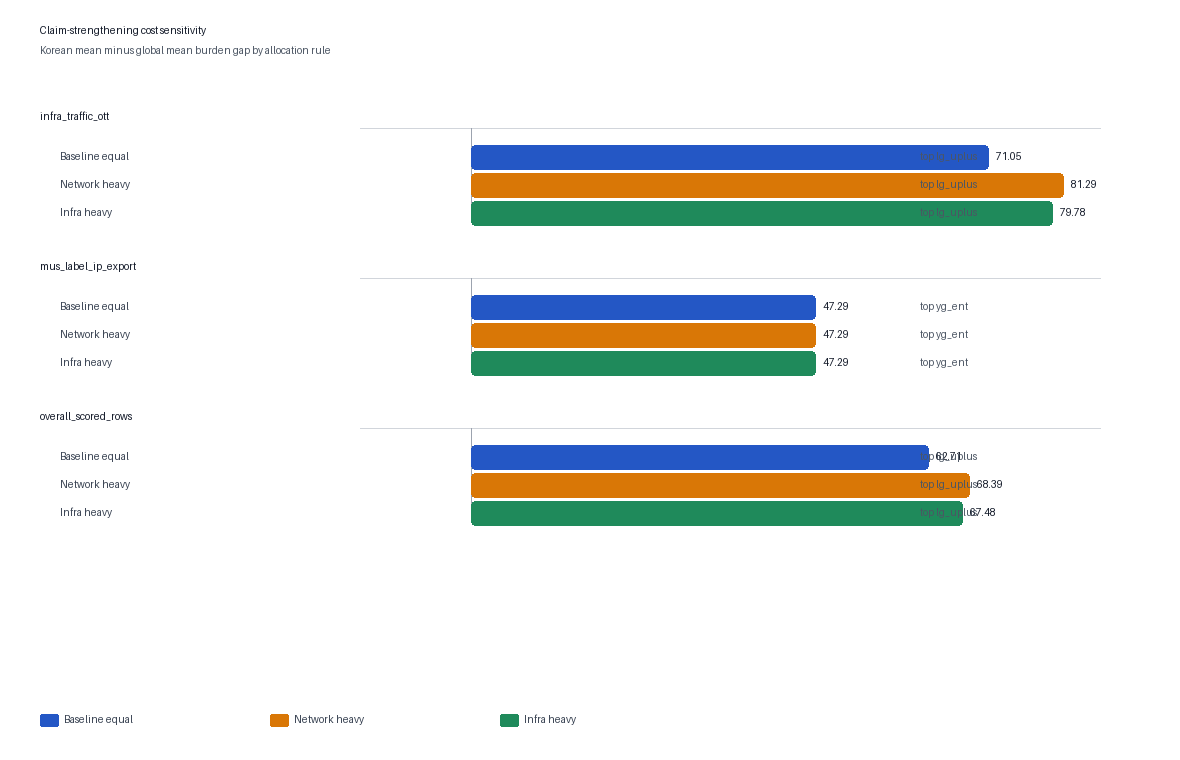
\includegraphics[width=0.88\textwidth]{outputs/figures/claim_strengthening/F_claim_cost_sensitivity.png}
\caption{비용배분 규칙 민감도 도표}
\label{fig:claim_cost_sensitivity}
\end{figure}

NET의 우선 검토 근거는 공통 표본과 불리한 민감도 조합에서도 유지된 상대적 점수 감소다. 기존 평균 8.57점과 종합점수 0.1000은 과거 시나리오 계산값으로 남겨 두고, 실제 성과는 비용절감·계약조건·투자회수·창작자 수취액으로 평가한다. BND·IPF·CBA 역시 기준값 재구성과 경계값 처리를 분리한 뒤 같은 지표로 비교한다.

\noindent{\small 근거: 표~\ref{tab:results_policy_scenarios}, 표~\ref{tab:policy_options}, 정책 실행 로드맵 항목, 표~\ref{tab:claim_cost_sensitivity}, 그림~\ref{fig:results_policy_sensitivity}, 그림~\ref{fig:results_cpii_robustness}, 그림~\ref{fig:claim_cost_sensitivity}, \nolinkurl{T_claim_cost_sensitivity.csv}.}\sourcefootnote{KOCCA 조사자료, KCC 공식 자료, OpenDART, SEC EDGAR, Cloudflare Radar(인증 수집 후보)}

\section{재현가능성과 정책판단의 함의}
재현성은 결과를 검토하고 정책을 갱신할 수 있게 하는 기반이다. 같은 원천자료와 전처리·정규화·집계 규칙에서 같은 결과가 나오는지 확인하고, 수치마다 원천과 계산 경로를 남긴다. 이 기록을 통해 연구자는 결과를 재검산하고, 실무자는 자료 추가나 가정 변경이 결론에 미치는 영향을 추적할 수 있다.

정책평가에서는 시행 전후 CPII와 하위지수, 비용회수액, 배분률을 같은 방식으로 반복 산출한다. 분기 모니터링은 이러한 변화가 지속되는지 확인하고, 자료나 비교조건이 달라졌을 때 그 영향을 구분하는 역할을 한다.

\noindent{\small 근거: \nolinkurl{final_reproducibility_checklist.csv}, \nolinkurl{row_level_lineage_summary.csv}, 표~\ref{tab:policy_options}.}\sourcefootnote{\texttt{source\_manifest.csv}, \texttt{project\_manifest.csv}}

\section{해석 범위와 후속 검증}
이 보고서의 결론은 공개자료에서 반복된 부담 방향과 같은 입력 조건에서 확인한 정책 간 상대 우위에 근거한다. 사건연구의 협의 표본 9/9는 사전추세 검정을 통과하지 못했고, 웹툰 위약 사건에서도 실제 사건과 유사한 사전 차이가 나타났다. 사건계수에서 인과효과를 식별하지 못했으므로, 해당 결과는 사건 전후의 변화와 식별조건을 점검하는 자료로 사용한다.

해외 한국 서비스의 직접 비용·계약자료와 웹툰 핵심축 관측은 추가 확보가 필요하다. 인프라의 위험-회수 사례는 KT가 양수이고 SK Telecom·LG Uplus가 음수여서 기업별 비용 경로를 구분해야 한다. 가격·품질·브랜드·네트워크 효과, 공시 가용성과 측정오차는 개별 효과 추정에서 함께 다룰 과제다. 관련 위약 검정, 관측가능성 목록과 대체 설명 점검 결과는 부록~\ref{app:evidence_scope}에 제시한다.

공통기간 비교와 대리지표 민감도를 함께 확인하면 어떤 부담 경로에 대응을 집중하고 어떤 자료를 먼저 보강할지 정할 수 있다. 카카오엔터테인먼트의 후속 분석은 멜론의 서비스별 손익·유지율, 외부 유통수익, 정산·계약자료를 같은 기간으로 연결하는 데 우선순위를 둔다.

\section{향후 연구}
향후 연구는 비교 표본과 관측기간을 넓히는 데서 시작한다. 우선 \nolinkurl{spotify@kr}의 한국 내 직접 규제·비용·공시자료, \nolinkurl{netflix@kr}의 한국 내 직접 망 부담·규제 집행자료, \nolinkurl{webtoon_serial_platform}의 동일 국가 장기 사전·사후 패널을 확보한다. 이를 통해 음악과 인프라는 같은 서비스의 비용·규제 경로를 구분하고, 웹툰은 사전추세와 비교군의 적합성을 다시 검정한다. 다음으로 준조세·규제방어 부담, 데이터결합·인앱결제 의존, 텐트폴 비용 상승, 창작자 협상 계약을 측정할 자료를 보강한다. FGI 부호화와 델파이 합의는 이러한 변수의 정의와 해석을 보완하는 근거로 구축한다.

국가별·기업별 표본과 공통 비교기간을 확장한 뒤, 사전추세와 비교군 적합성을 다시 검정해 분야별 순위와 정책별 비용·효과를 평가한다. CPII는 정기 갱신하는 모니터링 체계로 운영한다. 분기 자료가 쌓이면 정책 도입 전후의 변화를 누적 추세로 살필 수 있고, 국제 비교 표본을 넓히면 국내 비용 비대칭과 규제 적용 차이를 더 다양한 비교군에서 검증할 수 있다.

\appendix

\chapter{부록 개요}
부록에는 상세 방법론, 재현성 절차, 추가 비교분석, 변수 사전, 기업 비교기 설명과 사용 설명서를 수록한다. 계산 규칙은 방법론·변수 사전에서, 실제 스프레드시트 작업은 부록~\ref{app:simulator-manual}에서 확인할 수 있다. 결과의 적용 범위와 추가 검증은 부록~\ref{app:evidence_scope}에 정리했다.

\begin{itemize}[leftmargin=2.2em]
  \item \textbf{기업 비교 시뮬레이터와 점수 차이의 경제적 해석:} 2개 및 $n$개 기업 비교, 점수차 분해, 경제적 노출액 브리지, 가상 기업 수치 예시와 해석 한계를 제시한다.
  \item \textbf{데이터 재현성 프로토콜:} 원자료 수집, 정제, 병합, 결측 처리, 검산 절차를 다른 연구자가 반복할 수 있도록 단계별로 정리한다.
  \item \textbf{추가 비교분석:} 본문 결론을 보조하는 추가 민감도와 비교표를 정리한다.
  \item \textbf{변수 사전:} CPII, 회귀식, 시뮬레이터에 쓰이는 변수 정의와 전처리 규칙을 일괄 제시한다.
  \item \textbf{스프레드시트 사용 설명서:} 실제 시트·셀별 입력, 가상 예시 재현, 금액 해석, 민감도와 오류 해결, 저장·복원 절차를 설명한다.
  \item \textbf{자료 범위와 추가 검증:} 위약 사건 검정, 서비스별 관측가능성, 대체 설명과 후속 자료를 정리한다.
\end{itemize}

% AUTO-GENERATED by scripts/cpii_simulator/build_appendix.py; do not edit.
% Deterministic source provenance (SHA256):
% source-sha256: data/processed/cpii_simulator/examples/fictional_companies.csv 36c851ef130ca99f7e985116b01b1f50bffa3603801dabcddfe9bae60199a424
% source-sha256: outputs/tables/cpii_simulator/examples/company_ranking.csv fcce7b7945d1d710429a0b7995f6d479f1f14ae7261b9b28e4af0dbf46d9f309
% source-sha256: outputs/tables/cpii_simulator/examples/pair_gap_matrix.csv 7b632e471aa0d90f4587ae4e3ec946767a6b013fc87313bc4d0adeb3993addd4
% source-sha256: outputs/tables/cpii_simulator/examples/pair_gaps.csv 264e5d5feb75e4933460827f33706e46a92e40ae605ff65ced8558f36873126c
% source-sha256: outputs/tables/cpii_simulator/examples/pair_contributions.csv 755afa4162a3b0240adddf973c7136b320d38a2a32d97ad573d1f0f3d23f6e42
% source-sha256: outputs/tables/cpii_simulator/examples/economic_interpretations.csv af728bcf517b486544e41c63ade504407f94099fe739de3f3603b76461b1116c
% source-sha256: outputs/tables/cpii_simulator/examples/golden_equal_gap_summary.csv c989ac21688473bf9184d2d78d8d149b553f96d0c604d7dcf6c9cb216b00eefd
% source-sha256: outputs/tables/cpii_simulator/examples/sensitivity_summary.csv 49091be5635fd9c12acb029464a2b8da882ea62fcea4f56b740907d6c993f819
% source-sha256: data/processed/cpii_simulator/anchor/POOL_SCQ_P01_P99_EMP_RANK_V1.json 274a907a5b383a4c00a57927ccb46c1488e8bfdee9990a1ed87741ca4a769e6a

\chapter{회사 입력형 CPII 비교와 경제적 차이 해석}
\label{app:cpii_company_comparator}

\noindent\fbox{\parbox{0.96\textwidth}{\textbf{Research Beta 경고.} 방법론 설명용 합성자료이며 실제 기업에 대한 추정이 아님. 현재 고정 앵커의 결합 기준표본과 일부 feature의 지원도가 매우 낮으므로, 결과는 연구·전략분석 보조지표로만 사용한다. 차별·역차별·위법성·손해 또는 인과효과를 판정하지 않는다.}}

\section{세 점수체계와 해석 단위}
회사 입력형 비교기에서 서로 다른 세 수치를 같은 축으로 읽어서는 안 된다. 

\begingroup
\small
\setlength{\tabcolsep}{4pt}
\begin{longtable}{@{}L{3.2cm}L{2.8cm}L{8.3cm}@{}}
\caption{CPII 관련 세 점수체계의 구분}\label{tab:cpii_appendix_scale_distinction}\\
\toprule
수치 & 범위·부호 & 정확한 의미 \\
\midrule
\endfirsthead
\toprule
수치 & 범위·부호 & 정확한 의미 \\
\midrule
\endhead
회사별 CPII & $0$--$100$ & 고정 기준분포에서 feature별 부담 위치를 정해진 가중치로 합성한 회사별 구조적 부담점수. 기업 백분위가 아니다. \\
회사쌍 점수차 $\Delta\mathrm{CPII}_{A-B}$ & \(-100\)--\(+100\) & $\mathrm{CPII}(A)-\mathrm{CPII}(B)$이다. 양수는 A의 측정 부담 위치가 B보다 높고, 음수는 그 반대다. \\
legacy signed evidence score & \(-1\)--\(+1\) & 0을 중심으로 판단·증거를 코딩한 별도 지표다. feature 기반 CPII나 A-B 점수차가 아니며 같은 축·범례·해석 규칙을 쓰지 않는다. \\
\bottomrule
\end{longtable}
\endgroup

특히 $\Delta\mathrm{CPII}=0.10$점은 feature별 기준분포 위치 차이의 \textbf{가중합이 정확히 $0.001$}이라는 뜻이다($0.10/100=0.001$). 이는 비용 $0.1\%$, 매출 $0.1\%$, 회사 간 기업 백분위 $0.1\%$p를 뜻하지 않는다. 점수차는 먼저 feature 기여도로 분해한 뒤, 해당 원단위와 등록된 경제 노출기준이 있을 때만 채널별로 해석한다.

\section{고정 앵커와 운용 사양}
방법론 버전 \texttt{CPII\_FIRM\_INPUT\_EQW\_V1}은 고정 앵커 \texttt{POOL\_SCQ\_P01\_P99\_EMP\_RANK\_V1}을 사용한다. 입력 회사 집합을 추가·삭제·재정렬해도 기존 회사 점수는 바뀌지 않는다. 
현재 앵커에서 10개 활성 feature가 모두 관측된 결합 기준표본은 2/159행뿐이다. 저지원 활성 feature \texttt{cross\_market\_transfer\_index}, \texttt{foreign\_dependency\_ratio}의 합산 유효가중치는 22.22\%다. 따라서 회사 경험적 백분위, pair-gap 경험적 백분위, 산업 대표분포 주장은 비활성화한다.

운용 feature 구성은 $I_{\mathrm{reg}}$/$I_{\mathrm{risk}}$/$I_{\mathrm{market}}$ 순서로 3/4/3, 합계 10개다. 이 구성은 보고서의 더 넓은 이론 변수목록을 자동 대체하지 않는다.

\begin{align}
z_{ij} &= \mathcal{N}_{j}^{\mathrm{fixed}}\!\left(d_j x_{ij}\right), \\
I_{ik} &= \frac{100}{|J_k|}\sum_{j\in J_k} z_{ij}, \qquad k\in\{\mathrm{reg},\mathrm{risk},\mathrm{market}\}, \\
\mathrm{CPII}_i &= \frac{1}{3}\sum_k I_{ik}, \\
\Delta\mathrm{CPII}_{A-B} &= \mathrm{CPII}_A-\mathrm{CPII}_B =\sum_j 100w_j\left(z_{Aj}-z_{Bj}\right).
\end{align}
여기서 $d_j$는 부담 증가 방향을 맞추는 부호, $\mathcal{N}_{j}^{\mathrm{fixed}}$는 고정 앵커의 변환·1\%/99\% winsorization·경험순위 정규화, $w_j$는 하위지수 내부 동일가중과 세 축 동일가중을 전개한 유효 feature 가중치다.

\section{합성 회사 입력과 \texorpdfstring{$n$}{n}개 회사 비교}
\textbf{방법론 설명용 합성자료이며 실제 기업에 대한 추정이 아님.} 아래 네 회사는 원천 CSV에서 생성한 통제 합성 예시다. 회사명은 식별자일 뿐이며 값을 조회·추론·대체하지 않는다.

\begin{landscape}
\begingroup
\scriptsize
\setlength{\tabcolsep}{2.5pt}
\begin{longtable}{@{}L{1.2cm}L{4.1cm}L{1.7cm}L{1.0cm}L{2.1cm}L{2.1cm}L{2.1cm}L{2.1cm}@{}}
\caption{방법론 설명용 합성 회사의 10개 원단위 입력}\label{tab:cpii_appendix_synthetic_inputs}\\
\toprule
축 & 입력 feature & 단위 & 방향 & \WrapCell{\texttt{SYN-A}\\가온 콘텐츠} & \WrapCell{\texttt{SYN-B}\\누리 미디어} & \WrapCell{\texttt{SYN-C}\\다온 스토리} & \WrapCell{\texttt{SYN-D}\\라온 플레이} \\
\midrule
\endfirsthead
\toprule
축 & 입력 feature & 단위 & 방향 & \WrapCell{\texttt{SYN-A}\\가온 콘텐츠} & \WrapCell{\texttt{SYN-B}\\누리 미디어} & \WrapCell{\texttt{SYN-C}\\다온 스토리} & \WrapCell{\texttt{SYN-D}\\라온 플레이} \\
\midrule
\endhead
$I_{\mathrm{reg}}$ & \WrapCell{유효세율 격차\\\texttt{effective\_\allowbreak{}tax\_\allowbreak{}rate\_\allowbreak{}gap}} & 소수비율 & +1 & -0.0200 & -0.0550 & 0.0100 & -0.0050 \\
$I_{\mathrm{reg}}$ & \WrapCell{인프라 비용·해외의존 결합비율\\\texttt{infra\_\allowbreak{}dependency\_\allowbreak{}ratio}} & 소수비율 & +1 & 0.1332 & 0.0640 & 0.0986 & 0.1136 \\
$I_{\mathrm{reg}}$ & \WrapCell{네트워크 비용률\\\texttt{network\_\allowbreak{}cost\_\allowbreak{}ratio}} & 소수비율 & +1 & 0.1800 & 0.1050 & 0.1450 & 0.1600 \\
$I_{\mathrm{risk}}$ & \WrapCell{세전이익 기반 회수 대리값\\\texttt{cashflow\_\allowbreak{}recovery\_\allowbreak{}ratio}} & 배수 & -1 & 0.42 & 0.73 & 0.18 & 0.51 \\
$I_{\mathrm{risk}}$ & \WrapCell{자금조달비용 스프레드\\\texttt{funding\_\allowbreak{}cost\_\allowbreak{}spread}} & 소수비율 & +1 & 0.0120 & 0.0040 & 0.0180 & 0.0090 \\
$I_{\mathrm{risk}}$ & \WrapCell{투자 회수율\\\texttt{investment\_\allowbreak{}recovery\_\allowbreak{}ratio}} & 배수 & -1 & 3.20 & 4.10 & 2.65 & 3.55 \\
$I_{\mathrm{risk}}$ & \WrapCell{IP 자산화 결손\\\texttt{ip\_\allowbreak{}assetization\_\allowbreak{}gap}} & 소수비율 & +1 & 0.0800 & 0.0250 & 0.1100 & 0.0650 \\
$I_{\mathrm{market}}$ & \WrapCell{시장간 전이 대리지수\\\texttt{cross\_\allowbreak{}market\_\allowbreak{}transfer\_\allowbreak{}index}} & 0--1 지수 & +1 & 0.2800 & 0.1600 & 0.3400 & 0.2400 \\
$I_{\mathrm{market}}$ & \WrapCell{해외의존비율\\\texttt{foreign\_\allowbreak{}dependency\_\allowbreak{}ratio}} & 소수비율 & +1 & 0.7400 & 0.6100 & 0.6800 & 0.7100 \\
$I_{\mathrm{market}}$ & \WrapCell{비용 대비 설비투자 압박률\\\texttt{outflow\_\allowbreak{}to\_\allowbreak{}capex\_\allowbreak{}ratio}} & 배수 & +1 & 8.50 & 4.00 & 6.80 & 7.40 \\
\bottomrule
\end{longtable}
\endgroup
\end{landscape}

\begingroup
\small
\setlength{\tabcolsep}{4pt}
\begin{longtable}{@{}L{1.0cm}L{3.7cm}L{1.5cm}L{1.5cm}L{1.5cm}L{1.5cm}L{2.4cm}@{}}
\caption{합성 회사의 고정 앵커 점수와 부담순위}\label{tab:cpii_appendix_synthetic_ranking}\\
\toprule
순위 & 회사 & CPII & $I_{\mathrm{reg}}$ & $I_{\mathrm{risk}}$ & $I_{\mathrm{market}}$ & 관측/활성 feature \\
\midrule
\endfirsthead
\toprule
순위 & 회사 & CPII & $I_{\mathrm{reg}}$ & $I_{\mathrm{risk}}$ & $I_{\mathrm{market}}$ & 관측/활성 feature \\
\midrule
\endhead
1 & \WrapCell{\texttt{SYN-C}\\다온 스토리\\\texttt{foreign}} & 42.77 & 24.72 & 76.38 & 27.20 & 10/10 \\
2 & \WrapCell{\texttt{SYN-A}\\가온 콘텐츠\\\texttt{domestic}} & 39.90 & 12.74 & 73.36 & 33.59 & 10/10 \\
3 & \WrapCell{\texttt{SYN-D}\\라온 플레이\\\texttt{domestic}} & 35.98 & 11.02 & 69.38 & 27.55 & 10/10 \\
4 & \WrapCell{\texttt{SYN-B}\\누리 미디어\\\texttt{foreign}} & 32.22 & 5.09 & 65.06 & 26.50 & 10/10 \\
\bottomrule
\end{longtable}
\endgroup

\begingroup
\small
\setlength{\tabcolsep}{5pt}
\begin{longtable}{@{}L{3.0cm}L{2.0cm}L{2.0cm}L{2.0cm}L{2.0cm}@{}}
\caption{합성 회사 CPII 점수차 행렬(행 A $-$ 열 B, 점)}\label{tab:cpii_appendix_pair_matrix}\\
\toprule
행 $A$ $-$ 열 $B$ & \texttt{SYN-A} & \texttt{SYN-B} & \texttt{SYN-C} & \texttt{SYN-D} \\
\midrule
\endfirsthead
\toprule
행 $A$ $-$ 열 $B$ & \texttt{SYN-A} & \texttt{SYN-B} & \texttt{SYN-C} & \texttt{SYN-D} \\
\midrule
\endhead
\WrapCell{\texttt{SYN-A}\\가온 콘텐츠} & +0.00 & +7.68 & -2.87 & +3.91 \\
\WrapCell{\texttt{SYN-B}\\누리 미디어} & -7.68 & +0.00 & -10.55 & -3.77 \\
\WrapCell{\texttt{SYN-C}\\다온 스토리} & +2.87 & +10.55 & +0.00 & +6.78 \\
\WrapCell{\texttt{SYN-D}\\라온 플레이} & -3.91 & +3.77 & -6.78 & +0.00 \\
\bottomrule
\end{longtable}
\endgroup
표의 대각선은 0이고, 각 비대각 원소는 반대 방향 원소와 부호가 반대다. 순위와 행렬은 동일한 고정 앵커와 공통 10개 feature로 계산된다.

\section{2개 회사 상세 추적: SYN-A 대 SYN-B}
\texttt{SYN-A}와 \texttt{SYN-B}는 동일 cohort에서 비교 가능하며, 기준 점수차는 $\Delta\mathrm{CPII}_{A-B}=+7.68$점이다. 다음 표는 원단위 입력에서 고정 앵커 위치, 유효가중치, CPII 기여도까지 한 줄로 추적한다.

\begin{landscape}
\begingroup
\scriptsize
\setlength{\tabcolsep}{2.2pt}
\begin{longtable}{@{}L{0.8cm}L{3.9cm}L{1.4cm}L{1.4cm}L{2.0cm}L{1.5cm}L{1.5cm}L{1.5cm}L{1.8cm}@{}}
\caption{SYN-A 대 SYN-B의 feature별 점수차 분해}\label{tab:cpii_appendix_driver_trace}\\
\toprule
순위 & driver & 원값 A & 원값 B & 방향정렬 원차 & $z_A$ & $z_B$ & $w_j$ & 기여도(점) \\
\midrule
\endfirsthead
\toprule
순위 & driver & 원값 A & 원값 B & 방향정렬 원차 & $z_A$ & $z_B$ & $w_j$ & 기여도(점) \\
\midrule
\endhead
1 & \WrapCell{유효세율 격차\\\texttt{effective\_\allowbreak{}tax\_\allowbreak{}rate\_\allowbreak{}gap}\\$I_{\mathrm{reg}}$} & -0.0200 & -0.0550 & 0.0350 & 0.2534 & 0.1027 & 11.11\% & +1.67 \\
2 & \WrapCell{세전이익 기반 회수 대리값\\\texttt{cashflow\_\allowbreak{}recovery\_\allowbreak{}ratio}\\$I_{\mathrm{risk}}$} & 0.42 & 0.73 & 0.31 & 0.6755 & 0.4840 & 8.33\% & +1.60 \\
3 & \WrapCell{해외의존비율\\\texttt{foreign\_\allowbreak{}dependency\_\allowbreak{}ratio}\\$I_{\mathrm{market}}$} & 0.7400 & 0.6100 & 0.1300 & 0.2108 & 0.1024 & 11.11\% & +1.20 \\
4 & \WrapCell{자금조달비용 스프레드\\\texttt{funding\_\allowbreak{}cost\_\allowbreak{}spread}\\$I_{\mathrm{risk}}$} & 0.0120 & 0.0040 & 0.0080 & 0.7982 & 0.6579 & 8.33\% & +1.17 \\
5 & \WrapCell{비용 대비 설비투자 압박률\\\texttt{outflow\_\allowbreak{}to\_\allowbreak{}capex\_\allowbreak{}ratio}\\$I_{\mathrm{market}}$} & 8.50 & 4.00 & 4.50 & 0.2969 & 0.1927 & 11.11\% & +1.16 \\
6 & \WrapCell{인프라 비용·해외의존 결합비율\\\texttt{infra\_\allowbreak{}dependency\_\allowbreak{}ratio}\\$I_{\mathrm{reg}}$} & 0.1332 & 0.0640 & 0.0692 & 0.0714 & 0.0238 & 11.11\% & +0.53 \\
7 & \WrapCell{네트워크 비용률\\\texttt{network\_\allowbreak{}cost\_\allowbreak{}ratio}\\$I_{\mathrm{reg}}$} & 0.1800 & 0.1050 & 0.0750 & 0.0573 & 0.0260 & 11.11\% & +0.35 \\
8 & \WrapCell{시장간 전이 대리지수\\\texttt{cross\_\allowbreak{}market\_\allowbreak{}transfer\_\allowbreak{}index}\\$I_{\mathrm{market}}$} & 0.2800 & 0.1600 & 0.1200 & 0.5000 & 0.5000 & 11.11\% & +0.00 \\
9 & \WrapCell{투자 회수율\\\texttt{investment\_\allowbreak{}recovery\_\allowbreak{}ratio}\\$I_{\mathrm{risk}}$} & 3.20 & 4.10 & 0.90 & 0.6968 & 0.6968 & 8.33\% & +0.00 \\
10 & \WrapCell{IP 자산화 결손\\\texttt{ip\_\allowbreak{}assetization\_\allowbreak{}gap}\\$I_{\mathrm{risk}}$} & 0.0800 & 0.0250 & 0.0550 & 0.7637 & 0.7637 & 8.33\% & +0.00 \\
\midrule
\multicolumn{8}{r}{기여도 합계} & +7.678162 \\
\multicolumn{8}{r}{합계 $-$ 표시 전 원점수차 잔차} & -5.33e-15 \\
\bottomrule
\end{longtable}
\endgroup
\end{landscape}

절대기여도 상위 3개 driver는 유효세율 격차 +1.67점, 세전이익 기반 회수 대리값 +1.60점, 해외의존비율 +1.20점이다. 양의 기여는 A-B 점수차를 넓히고 음의 기여는 줄이며, 0 기여도도 원값 차이가 없다는 뜻은 아닐 수 있다. 고정 경험순위에서 같은 위치로 매핑되면 원값 차이가 있어도 점수 기여는 0이 된다.

\subsection{원단위 차이에서 경제량까지}
공통규모 상당액은 두 회사에 공통으로 적용한 노출기준에서 driver의 원단위 차이를 비교한다. 실제규모 차이는 회사별 수준과 회사별 노출액을 각각 결합하므로 공통규모 값과 다른 질문에 답한다. \texttt{scenario\_only}는 관측 손익이 아니라 명시적 가정에 따른 시나리오이며, \texttt{non\_monetizable}은 독립적·비중복 경제계수가 식별되지 않아 금액으로 바꾸지 않는다.

\begin{landscape}
\begingroup
\scriptsize
\setlength{\tabcolsep}{2pt}
\begin{longtable}{@{}L{4.3cm}L{3.1cm}L{3.1cm}L{4.1cm}L{4.1cm}L{2.5cm}@{}}
\caption{SYN-A 대 SYN-B의 경제해석 low/base/high(2025년 KRW, 억원)}\label{tab:cpii_appendix_economic_trace}\\
\toprule
driver & 해석 유형 & 노출기준 & 공통규모 low / base / high & 실제규모 low / base / high & 중복군 \\
\midrule
\endfirsthead
\toprule
driver & 해석 유형 & 노출기준 & 공통규모 low / base / high & 실제규모 low / base / high & 중복군 \\
\midrule
\endhead
\WrapCell{유효세율 격차\\\texttt{effective\_\allowbreak{}tax\_\allowbreak{}rate\_\allowbreak{}gap}} & 조건부 회계 상당액 & 양(+) 세전이익 & +34.65 / +38.50 / +42.35 & +54.90 / +61.00 / +67.10 & 조세부담 \\
\WrapCell{세전이익 기반 회수 대리값\\\texttt{cashflow\_\allowbreak{}recovery\_\allowbreak{}ratio}} & 조건부 성과 상당액 & 콘텐츠투자액 & +558.00 / +620.00 / +682.00 & +351.00 / +390.00 / +429.00 & 회수성 \\
\WrapCell{해외의존비율\\\texttt{foreign\_\allowbreak{}dependency\_\allowbreak{}ratio}} & 화폐환산 불가 & 적용 없음 & -- & -- & 네트워크·인프라 \\
\WrapCell{자금조달비용 스프레드\\\texttt{funding\_\allowbreak{}cost\_\allowbreak{}spread}} & 조건부 회계 상당액 & 평균 이자부부채 & +18.72 / +20.80 / +22.88 & +24.48 / +27.20 / +29.92 & 자금·IP \\
\WrapCell{비용 대비 설비투자 압박률\\\texttt{outflow\_\allowbreak{}to\_\allowbreak{}capex\_\allowbreak{}ratio}} & 화폐환산 불가 & 적용 없음 & -- & -- & 네트워크·인프라 \\
\WrapCell{인프라 비용·해외의존 결합비율\\\texttt{infra\_\allowbreak{}dependency\_\allowbreak{}ratio}} & 화폐환산 불가 & 적용 없음 & -- & -- & 네트워크·인프라 \\
\WrapCell{네트워크 비용률\\\texttt{network\_\allowbreak{}cost\_\allowbreak{}ratio}} & 조건부 회계 상당액 & 매출 & +810.00 / +900.00 / +990.00 & +297.00 / +330.00 / +363.00 & 네트워크·인프라 \\
\WrapCell{시장간 전이 대리지수\\\texttt{cross\_\allowbreak{}market\_\allowbreak{}transfer\_\allowbreak{}index}} & 가정 기반 시나리오 & 대상시장 매출 & +8.42 / +11.70 / +15.44 & +10.08 / +14.00 / +18.48 & 시장전이 \\
\WrapCell{투자 회수율\\\texttt{investment\_\allowbreak{}recovery\_\allowbreak{}ratio}} & 조건부 성과 상당액 & 콘텐츠투자액 & +1,620.00 / +1,800.00 / +1,980.00 & +306.00 / +340.00 / +374.00 & 회수성 \\
\WrapCell{IP 자산화 결손\\\texttt{ip\_\allowbreak{}assetization\_\allowbreak{}gap}} & 가정 기반 시나리오 & 매출 & +594.00 / +660.00 / +726.00 & +405.00 / +450.00 / +495.00 & 자금·IP \\
\bottomrule
\end{longtable}
\endgroup
\end{landscape}
모든 경제해석 행의 집계 규칙은 \texttt{never\_auto\_sum}이다. 조건부 회계 상당액, 조건부 성과 상당액, 시나리오 금액은 개념과 중복 family가 다르고 서로 원인·결과 관계일 수도 있으므로 합계 손실액처럼 자동 합산하지 않는다. low/base/high도 결정론적 입력·노출 가정 범위이며 신뢰구간이나 확률구간이 아니다.

\section{같은 점수차, 다른 경제적 크기: 골든 통제 예시}
두 골든 pair는 하나의 driver만 바꾸어 동일한 CPII 점수차를 만들지만 노출기준과 원단위가 다르다.

\begingroup
\small
\setlength{\tabcolsep}{4pt}
\begin{longtable}{@{}L{3.2cm}L{3.0cm}L{2.2cm}L{2.8cm}L{2.8cm}@{}}
\caption{동일 CPII 점수차의 네트워크·조달금리 경제량 대비}\label{tab:cpii_appendix_equal_gap_golden}\\
\toprule
통제 pair & 단일 변경 driver & $\Delta$CPII(점) & 공통 노출 base(억원) & 공통규모 base(억원) \\
\midrule
\endfirsthead
\toprule
통제 pair & 단일 변경 driver & $\Delta$CPII(점) & 공통 노출 base(억원) & 공통규모 base(억원) \\
\midrule
\endhead
\WrapCell{네트워크 비용률 통제\\\texttt{GOLD-N-A}\\\texttt{GOLD-N-B}} & 네트워크 비용률 & +1.3889 & 10,000.00 & 997.52 \\
\WrapCell{조달금리 통제\\\texttt{GOLD-F-A}\\\texttt{GOLD-F-B}} & 조달금리 스프레드 & +1.3889 & 1,000.00 & 2.00 \\
\bottomrule
\end{longtable}
\endgroup
두 pair의 점수차는 각각 1.3889점으로 같지만, 네트워크 비용률 채널의 공통규모 base는 약 997.52억원, 자금조달비용 스프레드 채널은 약 2.00억원이다. 전자는 후자의 약 498.95배다. 따라서 보편적인 ``CPII 1점당 원화'' 계수는 존재하지 않는다.

\section{민감도 판독과 한계}
\begingroup
\footnotesize
\setlength{\tabcolsep}{2pt}
\begin{longtable}{@{}L{2.5cm}L{1.5cm}L{2.8cm}L{1.5cm}L{2.0cm}L{3.8cm}@{}}
\caption{합성 회사 pair별 결정론적 민감도 범위}\label{tab:cpii_appendix_sensitivity}\\
\toprule
pair & 기준 gap & 민감도 구간 [min, max] & 부호 안정 & 양(+) 사양 비중 & 판독 \\
\midrule
\endfirsthead
\toprule
pair & 기준 gap & 민감도 구간 [min, max] & 부호 안정 & 양(+) 사양 비중 & 판독 \\
\midrule
\endhead
SYN-A–SYN-B & +7.68 & [-2.00, +14.32] & \texttt{no} & 83.33\% & 차이 불명확 \\
SYN-A–SYN-C & -2.87 & [-11.47, +4.39] & \texttt{no} & 16.67\% & 차이 불명확 \\
SYN-A–SYN-D & +3.91 & [-7.21, +11.14] & \texttt{no} & 83.33\% & 차이 불명확 \\
SYN-B–SYN-C & -10.55 & [-15.88, -3.52] & \texttt{yes} & 0.00\% & 시험 사양 내 방향 유지 \\
SYN-B–SYN-D & -3.77 & [-11.61, +3.22] & \texttt{no} & 16.67\% & 차이 불명확 \\
SYN-C–SYN-D & +6.78 & [-1.69, +12.69] & \texttt{no} & 83.33\% & 차이 불명확 \\
\bottomrule
\end{longtable}
\endgroup
선택 pair SYN-A–SYN-B의 범위는 -2.00점에서 +14.32점이며 0을 포함한다. 따라서 기준점수의 부호만으로 안정된 차이라고 결론내리지 않고 차이 불명확로 판독한다.

\begingroup\small
\begin{itemize}[leftmargin=2em,itemsep=0.15em,topsep=0.25em]
\item 민감도 [min, max] 구간은 입력 범위와 사전 정의 대체 사양을 통과시킨 결정론적 범위다. 신뢰구간·확률구간·예측구간이 아니며, 양(+) 사양 비중도 확률이 아니다.
\item 결합 기준표본이 얇으므로 회사 경험적 백분위, pair-gap 경험적 백분위, 산업 대표성은 주장하지 않는다. 저지원 feature의 가중치가 결과에 포함된다는 Research Beta 경고를 항상 함께 본다.
\item 합성 예시는 계산 재현성을 검증할 뿐 실제 회사, 산업 평균, 법적 차별·역차별, 위법성, 손해 또는 인과효과의 증거가 아니다.
\end{itemize}
\endgroup

% End of auto-generated CPII company-comparator appendix.


\chapter{재현성 프로토콜}
\section{자료 수집 및 정제 절차}
재현성 프로토콜은 공개원천의 수집부터 분석표 생성까지 같은 절차를 반복할 수 있도록 정리한 것이다. 원자료는 가공 전에 보존하고 가공본과 분리한다. 가상 사양, 부속 지수, FGI 부호화표, 델파이 중앙값·사분범위 시트, 엑셀 검증 기록은 각각 실제 관측자료와 구분해 관리한다.
\begin{enumerate}[label=\arabic*.]
  \item 원자료 다운로드 순서는 다음과 같이 고정한다. 첫째, 공표주기와 버전 관리가 가장 안정적인 정부·공공기관 자료를 수집한다. 둘째, OpenDART와 SEC EDGAR의 분기·연간 공시를 수집한다. 셋째, NAVER DataLab 등 인증 가능한 API 자료를 수집하고, Cloudflare Radar는 토큰 인증 실행 로그가 확보될 때 보조 트래픽 자료로 추가한다. 넷째, Circle Chart, 플랫폼 공개 랭킹·카탈로그, 공식 요금표를 수집한다. 다섯째, OECD, ITU, WIPO 등 국제 비교자료를 수집한다. 이 순서는 기준 표본과 통제변수를 먼저 고정한 후 고빈도 보조지표를 얹기 위한 것이다.
  \item 파일명 규칙은 원본과 가공본 모두에 동일하게 적용한다. 권장 형식은 \nolinkurl{<dataset_code>__<geo>__<platform>__<freq>__<period_start>_<period_end>__access<yyyymmdd>.<ext>}이다. 예시는 다음 두 형태를 기준으로 삼는다. \nolinkurl{kcc_mediause__kr__all__year__2019_2025__access20260328.pdf}, \nolinkurl{opendart__kr__kakao__quarter__2020Q1_2025Q4__access20260328.csv}.
  \item 날짜 표준화 규칙은 반드시 ISO 형식으로 고정한다. 일 단위는 \texttt{YYYY-MM-DD}, 월 단위는 \texttt{YYYY-MM}, 분기 단위는 \texttt{YYYYQq}를 사용한다. 사건연구용 표본은 추가로 \texttt{event\_date}, \texttt{event\_month}, \texttt{relative\_period}를 생성한다. 주간 자료는 해당 주의 종료일 기준으로 정렬하고, 월 또는 분기로 집계할 때는 종료일이 속한 기간에 배정한다.
  \item 통화 단위 변환 규칙은 모든 금액을 명목 원화(\texttt{KRW})로 통일한 뒤 필요 시 2025년 실질 원화로 재조정하는 2단계 구조를 따른다. 외화 공시값은 공식 월평균 환율 시계열을 사용해 원화로 환산하고, 연간 자료는 해당 연도 평균환율, 분기 자료는 분기 평균환율, 월 자료는 월평균 환율을 적용한다. 물가조정이 필요한 경우 기준연도 CPI로 나누어 실질값을 만든다. 원환산 전 금액과 환율 시리즈는 별도 열로 모두 보존한다.
  \item 플랫폼명과 서비스명 표준화 규칙은 하나의 표준 사전을 고정하는 방식으로 운영한다. 예를 들어 \texttt{YouTube}, \texttt{Youtube}, \texttt{유튜브}는 \texttt{youtube}, \texttt{YouTube Music}, \texttt{Youtube Music}, \texttt{유튜브뮤직}은 \texttt{youtube\_music}, \texttt{NAVER WEBTOON}과 \texttt{네이버웹툰}은 \texttt{naver\_webtoon}으로 통일한다. 법인명과 서비스명은 분리 열로 관리하며, 비교군 매핑표에는 \texttt{firm\_std}, \texttt{service\_std}, \texttt{country\_std}, \texttt{sector\_std}를 반드시 둔다.
  \item 중복 제거 규칙은 ``같은 표준 키에 대해 가장 공식성이 높고 접근일이 명확한 관측만 남긴다''로 고정한다. 원천 우선순위는 공식 API $>$ 공식 CSV/XLS $>$ 공식 PDF 수기전사 $>$ 보조 웹표이다. 동일 원천 내 중복은 최신 정정본을 남기고, 서로 다른 원천이 동일 값을 제공할 때는 기준 원천 하나만 선택해 남긴다. 중복 제거 후 삭제된 행 수와 사유는 \texttt{dedup\_log}에 기록한다.
  \item 결측치 처리 규칙은 세 단계로 고정한다. 첫째, 변수 사전에 사전 지정된 공개 대체지표가 있으면 그 값으로 대체한다. 둘째, 동일 분기 또는 동일 월의 동원천 파생 산식으로 계산 가능하면 직접 계산한다. 셋째, 공표주기 차이 때문에 생긴 결측만 직전 1기간까지 이월한다. 그 이후에도 값이 없으면 결측으로 유지하고, 분석 테이블에는 \texttt{missing\_flag}를 별도 저장한다.
  \item 이상치 처리 규칙은 입력오류 제거와 통계적 완화를 구분한다. 입력오류는 단위 착오, 자리수 오류, 부호 오류를 교정 또는 제거한다. 통계적 이상치는 로그변환 대상은 변환 후 분포를 점검하고, 기준 사양에서는 pooled distribution 기준 1\%/99\% winsorization을 적용한다. 사건 표본이나 소표본 강건성 검정에는 5\%/95\% winsorization을 병행한다. 원시값, winsorized 값, 변환값을 모두 저장하여 추적 가능하게 한다.
  \item 병합 키는 분석 단위별로 고정한다. 플랫폼-월 패널은 \texttt{service\_std + year\_month}, 플랫폼-분기 패널은 \texttt{service\_std + year\_quarter}, 작품-분기 패널은 \nolinkurl{title_std + service_std + year_quarter}, 분야-분기 패널은 \texttt{sector\_std + year\_quarter}, 사건연구 테이블은 \nolinkurl{event_id + relative_period + unit_id}를 기본 키로 사용한다. 병합 전에 각 키의 유일성 검정을 수행하고, 일대다 병합은 사전에 정의한 경우에만 허용한다.
  \item 최종 분석 테이블 생성 규칙은 네 개의 마스터 테이블을 만든 뒤 그 하위 결과물을 파생하는 방식으로 고정한다. 첫째, \texttt{source\_manifest}는 원천 URL, 접근일, 파일명, 공표주기, 라이선스를 담는다. 둘째, \nolinkurl{panel_platform_month}는 음악·인프라의 월별 분석용 테이블이다. 셋째, \nolinkurl{panel_platform_quarter}와 \nolinkurl{panel_title_quarter}는 웹툰 및 재무 분석용 분기 테이블이다. 넷째, \nolinkurl{panel_sector_quarter}는 CPII 산출의 기준 테이블이다. 모든 회귀와 지수 계산은 이 네 개 마스터 테이블에서만 시작하고, 중간 가공 산출물은 별도 저장하되 원본을 덮어쓰지 않는다.
\end{enumerate}

\section{재현성 점검표}
\begin{enumerate}[label=\arabic*.]
  \item 모든 원자료 파일에 URL, 접근일, 파일명, 버전 또는 공표일이 기록되어 있는가.
  \item 원자료 폴더와 가공 폴더가 분리되어 있으며 원본이 보존되어 있는가.
  \item 파일명이 동일 규칙을 따르고 기간과 접근일을 포함하는가.
  \item 모든 날짜가 \texttt{YYYY-MM-DD}, \texttt{YYYY-MM}, \texttt{YYYYQq} 규칙으로 표준화되었는가.
  \item 외화 금액이 공식 환율 시계열을 통해 원화로 환산되었고 환산 전 값이 보존되어 있는가.
  \item 플랫폼명, 서비스명, 법인명이 표준 사전으로 매핑되었는가.
  \item 중복 제거 로그와 결측치 처리 로그가 별도 파일로 남아 있는가.
  \item 이상치 처리 전후 값이 모두 저장되어 있으며 winsorization 기준이 명시되어 있는가.
  \item 병합 키 유일성 검정 결과가 저장되어 있는가.
  \item 최종 분석 테이블이 \nolinkurl{panel_platform_month}, \nolinkurl{panel_platform_quarter}, \nolinkurl{panel_title_quarter}, \nolinkurl{panel_sector_quarter}로 구분되어 있는가.
\end{enumerate}

\section{분석표·그림의 설계 목록}
\label{app:result_design_inventory}
다음 목록은 초기 분석 설계의 표 12종·그림 10종 식별번호와 목적을 정리한다. 광의의 후보변수와 실측 실행 사양을 구분하며, 실제 결과표와 추가 검증표는 본문의 실증분석 결과 장에 제시한다. T09와 F04의 기존 평균은 분야별 가용기간 기준이고, 공통기간 평균은 별도 민감도 표로 제시한다.

\begingroup
\scriptsize
\begin{summarylist}
  \item \textbf{T01 / 표본 프레임 및 관측단위 고정표}. 장/절: 연구 질문과 판정 기준 / 분석 단위와 표본 프레임. 데이터: \texttt{sector\_std}, \texttt{platform\_std}, \texttt{title\_std}, \texttt{year\_quarter}, \texttt{month\_id}, \texttt{event\_id}. 계산 방식: 분야별로 플랫폼-월, 분야-분기, 작품-분기, 사건-월 단위의 관측치 수, 커버리지, 공통 지지구간을 집계한다. 해석 포인트: 어떤 결과가 어떤 단위에서 판정되는지, 서로 다른 표본을 직접 비교하면 안 되는 구간이 어디인지 드러낸다.
  \item \textbf{T02 / 공개데이터 원천 및 재현성 등급표}. 장/절: 데이터와 재현성 원칙 / 공개데이터 원천 전수조사. 데이터: 기관별 자료명, 접근 방식, 공표 주기, 시계열 길이, API 여부, 공개성 등급. 계산 방식: 원천별로 재현성, 연속성, 비교 가능성 점수를 부여해 A/B/C 등급으로 정리한다. 해석 포인트: 최종 수치가 어떤 공개원천에 주로 의존하는지와 대체지표 사용이 필요한 구간을 한눈에 보여준다.
  \item \textbf{T03 / CPII 변수 사전 요약표}. 장/절: 데이터와 재현성 원칙 / 공개데이터 사용 원칙. 데이터: 핵심 27개 변수, 단위, 자료원, 기대 부호, 결측 규칙. 계산 방식: 변수 사전에서 핵심 변수만 추려 하위 지수별 묶음, 원시/가공 구분, 기대 부호를 요약한다. 해석 포인트: 독자가 뒤의 식과 결과를 읽기 전에 어떤 신호가 어느 하위 지수로 들어가는지 이해할 수 있게 한다.
  \item \textbf{T04 / CPII 집계 규칙 비교표}. 장/절: CPII 설계 / 권고안과 대체 사양. 데이터: 로그변환 규칙, winsorization 규칙, 정규화 방식, 가중치 방식. 계산 방식: 기준 사양과 대체 사양 A/B를 행 단위로 정리하고 각 조합의 장단점과 사용 목적을 비교한다. 해석 포인트: 결과가 어떤 방법 선택에 민감한지 해석할 기준선을 제공한다.
  \item \textbf{T05 / 제도적 불평등 지수 구성표}. 장/절: CPII 설계 / 제도적 불평등 지수 설계. 데이터: \texttt{reg\_lag\_months}, \texttt{obligation\_count}, \texttt{reporting\_burden\_days}, \texttt{compliance\_cost\_ratio}, \texttt{network\_cost\_ratio}, \texttt{effective\_tax\_rate\_gap}, \texttt{infra\_dependency\_ratio}. 계산 방식: 다섯 구성요소와 대응 원시변수, 계산식 1안과 2안을 함께 표시하고 기준 사양을 표시한다. 해석 포인트: CPII 상승이 규제 시차, 집행 격차, 망 비용, 조세, 절차 중 어느 축에서 비롯되는지 추적 가능하게 만든다.
  \item \textbf{T06 / 리스크 및 비용 비대칭 지수 구성표}. 장/절: CPII 설계 / 리스크 및 비용 비대칭 지수 설계. 데이터는 \texttt{content\_investment\_ratio}, \texttt{investment\_recovery\_ratio}, \texttt{cashflow\_recovery\_ratio}, \texttt{settlement\_delay\_days}를 기본 축으로 둔다. 보조 축으로 \texttt{funding\_cost\_spread}, \texttt{ip\_assetization\_gap}, \texttt{creator\_share\_ratio}를 추가해 회수 부족분과 조달 불리함을 함께 정리한다. 계산 방식: 회수 부족분, 정산 지연, 자금조달 스프레드, IP 자산화 결손, 배분률 미달분을 부분지수와 함께 표준화한다. 해석 포인트: 비용과 리스크가 매출 규모가 아니라 회수 실패와 자금조달 불리함으로 계량된다는 점을 분명히 한다.
  \item \textbf{T07 / 시장 지배력 전이 지수 구성표}.\\ 장/절: CPII 설계 / 시장 지배력 전이 지수 설계. 데이터는 전이, 결합, 집중, 락인, 해외의존, 잠식속도를 대표하는 핵심 지표 묶음이다. 상세 변수명은 변수 사전과 본 표 본문에서 다시 제시한다. 계산 방식: 전이, 집중, 락인, 해외의존, 잠식속도의 다섯 부분지수와 대응 지표를 묶어 제시한다. 해석 포인트: 단순 점유율이 아니라 지배력이 인접 시장으로 옮겨가는 구조를 계량하고 있음을 보여준다.
  \item \textbf{T08 / 기초통계 및 분위수 요약표}. 장/절: 실증 결과 / 기초통계. 데이터: 최종 분석 테이블의 종속변수, 핵심 설명변수, 통제변수, CPII 및 하위 지수. 계산 방식: 분야별로 평균, 표준편차, 중위값, 25/75 분위, 최소값, 최대값, 관측치 수를 계산한다. 해석 포인트: 극단치, 표본 불균형, 단위 이상 여부를 먼저 점검하고 이후 회귀와 지수 해석의 기초 분포를 제공한다.
  \item \textbf{T09 / 하위 지수 분야별 절대수준 표}. 장/절: 실증 결과 / CPII 산출 결과. 데이터: $I^{\mathrm{reg}}_{s,q}$, $I^{\mathrm{risk}}_{s,q}$, $I^{\mathrm{market}}_{s,q}$, 공통 기간 $Q_{\mathrm{common}}$. 계산 방식: 분야별 가용기간 평균을 계산하고, 각 분야에서 가장 크게 나타나는 부담 채널을 함께 적는다. 해석 포인트: 어느 분야에서 어떤 채널의 절대 부담 수준이 높은지 바로 읽을 수 있다.
  \item \textbf{T10 / 하위 지수 0기준 상대부담 재표현표}. 장/절: 실증 결과 / CPII 산출 결과. 데이터: 분야별 평균 $I^{\mathrm{reg}}$, $I^{\mathrm{risk}}$, $I^{\mathrm{market}}$. 계산 방식: 각 평균값에서 50을 빼서 0 기준 값으로 재표현한다. 해석 포인트: 양수는 고정 참조분포의 50점을 넘는 상태, 음수는 그 아래에 있는 상태임을 직관적으로 보여 준다.
  \item \textbf{T11 / 사건연구 및 강건성 추정치 요약표}. 장/절: 실증 결과 / 음악·웹툰 및 스토리·디지털 인프라 결과. 데이터: 모형별 추정계수, 표준오차, 사전추세 검정값, 표본 수, 사양 코드. 계산 방식: 분야별 핵심 종속변수에 대해 기본 추정식과 대체 추정식의 계수, 유의성, 사전추세 통과 여부를 정리한다. 해석 포인트: 결론이 특정 식별전략에만 의존하는지, 혹은 동일한 방향으로 반복되는지 판별한다.
  \item \textbf{T12 / 정책 시나리오 결과 및 민감도 요약표}. 장/절: 실증 결과 / 정책 시나리오 결과. 데이터: 시나리오별 입력 가정, 기준 점수, 변화 후 점수, 회복 매출, 투자재원, 공유율 개선폭. 계산 방식: 각 시나리오별로 기준값, 충격값, 출력값, 민감도 상·하한을 계산해 비교한다. 해석 포인트: 어떤 정책이 CPII 하락과 수익 회복에 가장 큰 기여를 하는지 우선순위를 정할 수 있다.
  \item \textbf{F01 / 데이터 수집-정제-지수 산출 파이프라인 순서도}. 장/절: 재현성 부록 / 재현 가능한 계산 절차. 데이터: 원자료 수집 순서, 정제 규칙, 정규화, 집계, 검산 단계. 계산 방식: 단계별 입력과 출력 파일을 화살표 다이어그램으로 연결하고 각 단계에 대응하는 체크식을 붙인다. 해석 포인트: 다른 연구자가 어떤 순서로 코드를 실행해야 하는지와 오류 검산이 어디서 수행되는지 즉시 파악할 수 있다.
  \item \textbf{F02 / CPII 시계열 선그래프}. 장/절: 실증 결과 / CPII 산출 결과. 데이터: 분기별 $\mathrm{CPII}_{s,q}$, 필요 시 4분기 이동평균. 계산 방식: 세 분야의 CPII를 동일 축 선그래프로 그리고 필요 시 이동평균선을 병기한다. 해석 포인트: 상승·하락 추세, 구조적 전환점, 분야 간 추세 차이를 가장 직관적으로 보여준다.
  \item \textbf{F03 / 하위 지수 분해 누적막대그래프}. 장/절: 실증 결과 / CPII 산출 결과. 데이터: $I^{\mathrm{reg}}$, $I^{\mathrm{risk}}$, $I^{\mathrm{market}}$의 분야별 평균 또는 특정 분기 값. 계산 방식: 분야별 또는 핵심 분기별로 세 하위 지수를 누적막대로 쌓아 총 CPII와 함께 표시한다. 해석 포인트: 높은 총점이 규제 채널인지, 비용 리스크 채널인지, 시장 전이 채널인지 분해해서 해석할 수 있다.
  \item \textbf{F04 / 분야별 평균 비교 막대그래프}. 장/절: 실증 결과 / CPII 산출 결과. 데이터: 가용기간 평균 CPII 및 하위지수. 공통기간과 불확실성은 별도 검증 항목이다. 계산 방식: 분야별 평균 막대와 오차막대를 함께 그리거나 하위 지수별 묶음 막대그래프로 제시한다. 해석 포인트: 텍스트 표보다 빠르게 어느 분야가 상대적으로 높은지, 차이가 통계적으로 불안정한지 확인할 수 있다.
  \item \textbf{F05 / 음악 분야 사건 전후 변화 그래프}. 장/절: 실증 결과 / 음악 분야 결과. 데이터: 음악 분야 사건시점별 $\hat{\beta}_{\tau}$, 신뢰구간, 사건 더미, 종속변수 시계열. 계산 방식: Event Study 계수 플롯 또는 사건 전후 평균 궤적 그래프로 그린다. 해석 포인트: 사전추세가 평평한지, 사건 이후 음원 점유율·검색점유율·회수율이 어떻게 바뀌는지 보여준다.
  \item \textbf{F06 / 웹툰 및 스토리 분야 사건 전후 변화 그래프}. 장/절: 실증 결과 / 웹툰 및 스토리 결과. 데이터: 작품-분기 또는 플랫폼-분기 사건계수, \texttt{creator\_share\_ratio}, \texttt{title\_survival\_ratio}, \texttt{local\_ip\_topN\_share}. 계산 방식: 사건 전후 계수 플롯 또는 평균 궤적을 그리고 작품군/플랫폼군별로 색을 구분한다. 해석 포인트: 웹툰 및 스토리 분야에서 노출, 배분률, 회수율이 충격 전후 어떻게 달라지는지와 사전추세 위반 여부를 동시에 확인한다.
  \item \textbf{F07 / 디지털 인프라 비용압력-불평등 관계 그래프}. 장/절: 실증 결과 / 디지털 인프라 결과. 데이터는 트래픽 비용압력, 네트워크 비용률, CAPEX 잠식비율, $\mathrm{CPII}$다. 계산 방식: 산점도와 적합선을 사용하거나 부분회귀 잔차도 형태로 제시한다. 해석 포인트: 트래픽 비용압력이 커질수록 불평등 점수가 높아지는지와 이상 관측치가 있는지를 보여준다.
  \item \textbf{F08 / 핵심 변수 상관구조 히트맵}. 장/절: 실증 결과 / 기초통계. 데이터: 정규화된 핵심 변수, 하위 지수, 주요 종속변수. 계산 방식: 피어슨 또는 스피어만 상관계수를 계산해 히트맵으로 표시한다. 해석 포인트: 특정 채널이 거의 동일한 정보를 반복하는지, 혹은 서로 독립적인 채널인지 확인할 수 있다.
  \item \textbf{F09 / 기준 사양-대체 사양 비교 차트}. 장/절: 실증 결과 / CPII 산출 결과. 데이터: 기준 사양 CPII, 대체 사양 A/B CPII, 순위 자료. 계산 방식: 기준 사양과 대체 사양의 점수 또는 순위를 산점도, slope chart, 혹은 rank scatter로 비교한다. 해석 포인트: 방법을 바꿔도 순위와 결론이 유지되는지, 특정 분야만 민감한지를 한 번에 파악할 수 있다.
  \item \textbf{F10 / 정책 시나리오 민감도 차트}. 장/절: 실증 결과 / 정책 시나리오 결과. 데이터: 시나리오별 탄력성, 변화 후 CPII, 회복 매출, 비용 회수액, 공유율 개선폭. 계산 방식: 토네이도 차트 또는 스파이더 차트로 입력값 변화가 출력값에 미치는 영향을 시각화한다. 해석 포인트: 어떤 정책이 기본 가정에 민감한지와 어떤 정책이 비교적 안정적으로 효과를 내는지 구분할 수 있다.
\end{summarylist}
\endgroup

\section{재현 절차 요약 목록}
\begin{enumerate}[label=\arabic*.]
  \item 원자료 다운로드 순서 고정
  \item 파일명 규칙 고정
  \item 날짜 표준화 규칙 고정
  \item 통화 단위 변환 규칙 고정
  \item 플랫폼명·서비스명 표준화 규칙 고정
  \item 중복 제거 규칙 고정
  \item 결측치 처리 규칙 고정
  \item 이상치 처리 규칙 고정
  \item 병합 키 정의 고정
  \item 최종 분석 테이블 생성 규칙 고정
\end{enumerate}

\section{재현 가능한 계산 절차}
CPII는 방향성 통일, 로그변환, 이상치 처리, 정규화, 하위 지수 계산, 가중합, 0--100 환산의 순서로 계산한다. 이어서 분야·시계열 비교와 민감도 분석을 수행한다. 동일한 자료와 규칙을 적용하면 각 단계의 중간 산출물도 같아야 한다.

\begin{equation}
\label{eq:cpii_pipeline}
\begin{aligned}
\{x_{j,s,q}\} &\rightarrow \{x^{\star}_{j,s,q}\} \rightarrow \{u_{j,s,q}\} \rightarrow \{u^{W}_{j,s,q}\} \rightarrow \{\widetilde{x}_{j,s,q}\} \\
&\rightarrow \{C^{\ell}_{s,q}\} \rightarrow \{I^{\mathrm{reg}}_{s,q}, I^{\mathrm{risk}}_{s,q}, I^{\mathrm{market}}_{s,q}\} \rightarrow S^{\mathrm{raw}}_{s,q} \rightarrow \mathrm{CPII}_{s,q}
\end{aligned}
\end{equation}

\begin{align}
d_j &=
\begin{cases}
1, & \text{if variable } j \text{ increases inequality} \\
-1, & \text{if variable } j \text{ reduces inequality}
\end{cases} \\
x^{\star}_{j,s,q} &= d_j x_{j,s,q} \\
u_{j,s,q} &=
\begin{cases}
\mathcal{L}_{+}(x^{\star}_{j,s,q}), & j \in J_{\log}^{+} \\
\mathcal{L}_{\pm}(x^{\star}_{j,s,q}), & j \in J_{\log}^{\pm} \\
x^{\star}_{j,s,q}, & \text{otherwise}
\end{cases} \\
u^{W}_{j,s,q} &= \min\!\left\{\max\!\left(u_{j,s,q}, P_{1}(u_j)\right), P_{99}(u_j)\right\} \\
\widetilde{x}_{j,s,q} &= \frac{\mathrm{rank}(u^{W}_{j,s,q})-1}{N_j-1} \label{eq:cpii_preprocess_steps}
\end{align}

여기서 $P_{1}(u_j)$와 $P_{99}(u_j)$는 변수 $j$의 pooled sector-quarter 분포의 1백분위와 99백분위이며, $N_j$는 해당 변수의 유효 관측치 수이다. 또한 하위 지수 내부의 실제 관측 집합을 $M_{k,s,q}\subseteq J_k$로 두면 결측 재정규화 가중치는 다음과 같이 정의한다.

\begin{align}
\omega'_{j,k,s,q} &=
\begin{cases}
\dfrac{\omega_{j,k}}{\sum_{h \in M_{k,s,q}}\omega_{h,k}}, & j \in M_{k,s,q} \\
0, & j \notin M_{k,s,q}
\end{cases} \\
I^{k}_{s,q} &= 100 \times \sum_{j \in M_{k,s,q}} \omega'_{j,k,s,q}\widetilde{x}_{j,s,q}, \qquad k \in \{\mathrm{reg},\mathrm{risk},\mathrm{market}\} \\
S^{\mathrm{raw}}_{s,q} &= \lambda_{\mathrm{reg}}\frac{I^{\mathrm{reg}}_{s,q}}{100} + \lambda_{\mathrm{risk}}\frac{I^{\mathrm{risk}}_{s,q}}{100} + \lambda_{\mathrm{market}}\frac{I^{\mathrm{market}}_{s,q}}{100} \\
\mathrm{CPII}_{s,q} &= 100 \times S^{\mathrm{raw}}_{s,q} \label{eq:cpii_aggregation_steps}
\end{align}

\subsection{절차}
아래 절차는 CPII를 계산할 때 고정해야 하는 입력값, 산출물, 대표 오류를 단계별로 정리한 것이다.
\begingroup
\footnotesize
\begin{summaryenum}
  \item \textbf{원시 변수 방향성 통일}. 입력값은 원자료 $x_{j,s,q}$와 변수별 부호 코드북 $d_j$다. $x^{\star}_{j,s,q}=d_j x_{j,s,q}$를 적용하여 모든 변수가 ``값이 클수록 구조적 불평등 심화'' 방향을 갖도록 재부호화한다. 파생형 결손지표는 원시 변수 대신 $g^{\mathrm{share}}$, $g^{\mathrm{eros}}$처럼 경제적 shortfall 식을 먼저 계산한 뒤 같은 방향성을 부여한다. 산출물은 $x^{\star}_{j,s,q}$이며, 대표 오류는 변수별 부호 사전 불일치, shortfall 식 누락, 음수 부호를 두 번 반전시키는 오류다.
  \item \textbf{로그변환}. 입력값은 $x^{\star}_{j,s,q}$와 로그대상 집합 $J_{\log}^{+}$, $J_{\log}^{\pm}$다. $j \in J_{\log}^{+}$이면 $\mathcal{L}_{+}(x)=\log(1+x)$, $j \in J_{\log}^{\pm}$이면 $\mathcal{L}_{\pm}(x)=\operatorname{sgn}(x)\log(1+|x|)$를 적용하고 그 외는 원척도를 유지하여 $u_{j,s,q}$를 만든다. 산출물은 $u_{j,s,q}$이며, 대표 오류는 음수값에 일반 로그를 적용하는 오류, signed-log 대신 절댓값 로그를 적용하는 오류, 로그대상 변수 목록 오기재다.
  \item \textbf{정규화}. 입력값은 $u_{j,s,q}$와 pooled 분포의 분위수 정보다. 먼저 명백한 단위오류를 제거하고 $u^{W}_{j,s,q}=\min\{\max(u_{j,s,q},P_{1}(u_j)),P_{99}(u_j)\}$로 winsorization을 적용한다. 이후 기준 사양은 $\widetilde{x}_{j,s,q}=(\mathrm{rank}(u^{W}_{j,s,q})-1)/(N_j-1)$로 경험적 분위수 정규화를 수행한다. 산출물은 $\widetilde{x}_{j,s,q}\in[0,1]$이며, 대표 오류는 winsorization 이전과 이후 데이터가 뒤섞이는 오류, 정렬 기준 오기재, 동일값 처리 방식 불일치, $N_j=1$인 변수를 그대로 정규화하는 오류다.
  \item \textbf{하위 지수 계산}. 입력값은 $\widetilde{x}_{j,s,q}$, 부분지수 정의, 내부 가중치 $\omega_{j,k}$다. 각 분야 정의에 따라 $C^{\mathrm{lag}}$, $C^{\mathrm{rec}}$, $C^{\mathrm{transfer}}$ 등 부분지수를 먼저 계산한 뒤, 관측 가능한 항목 집합 $M_{k,s,q}$에 대해 재정규화 가중치 $\omega'_{j,k,s,q}$를 적용하여 $I^{k}_{s,q}=100\sum_{j \in M_{k,s,q}}\omega'_{j,k,s,q}\widetilde{x}_{j,s,q}$를 산출한다. 산출물은 $I^{\mathrm{reg}}_{s,q}$, $I^{\mathrm{risk}}_{s,q}$, $I^{\mathrm{market}}_{s,q}$이며, 대표 오류는 누락 항목 발생 시 가중치 재정규화 누락, 구성요소와 원시변수를 중복 합산하는 오류, 40\% 이상 결측인데도 지수를 산출하는 오류다.
  \item \textbf{최종 가중합}. 입력값은 세 하위 지수와 상위 가중치 $\lambda_k$다. $S^{\mathrm{raw}}_{s,q}=\lambda_{\mathrm{reg}}I^{\mathrm{reg}}_{s,q}/100+\lambda_{\mathrm{risk}}I^{\mathrm{risk}}_{s,q}/100+\lambda_{\mathrm{market}}I^{\mathrm{market}}_{s,q}/100$를 계산하고, 기준 사양은 $\lambda_k=1/3$으로 둔다. 산출물은 $S^{\mathrm{raw}}_{s,q}\in[0,1]$이며, 대표 오류는 상위 가중치 합이 1이 아닌 상태로 계산하는 오류, 하위 지수를 100으로 나누지 않아 이중 스케일링이 발생하는 오류다.
  \item \textbf{0--100 재스케일링}. 입력값은 $S^{\mathrm{raw}}_{s,q}$다. $\mathrm{CPII}_{s,q}=100\times S^{\mathrm{raw}}_{s,q}$로 환산하고, 해석 구간 표에 따라 라벨을 부여한다. 본 연구의 기준 사양에서는 하위 지수가 이미 0--100이므로 최종 환산은 상위 가중합을 사람이 읽기 쉬운 0--100 지수로 표시하는 단계다. 산출물은 최종 $\mathrm{CPII}_{s,q}\in[0,100]$이며, 대표 오류는 100을 두 번 곱하거나 아예 곱하지 않는 오류, 반올림 전에 라벨을 부여하여 경계값 판정이 달라지는 오류다.
  \item \textbf{분야별 비교}. 입력값은 공통 관측구간 $Q_{\mathrm{common}}$와 분야 집합 $\mathcal{S}$다. 동일 기간 비교만 허용하며, $Q_{\mathrm{common}}=\bigcap_{s \in \mathcal{S}}Q_s$를 정의하고 $\bar{\mathrm{CPII}}^{\mathrm{cmp}}_{s}=|Q_{\mathrm{common}}|^{-1}\sum_{q \in Q_{\mathrm{common}}}\mathrm{CPII}_{s,q}$ 및 $\Delta^{\mathrm{sector}}_{s,s'}=\bar{\mathrm{CPII}}^{\mathrm{cmp}}_{s}-\bar{\mathrm{CPII}}^{\mathrm{cmp}}_{s'}$를 계산한다. 산출물은 분야 평균과 분야 간 격차이며, 대표 오류는 서로 다른 표본기간을 직접 비교하는 오류, 사건표본과 정기패널을 혼합 비교하는 오류, 분기 수가 너무 적은데도 평균 비교를 수행하는 오류다.
  \item \textbf{시계열 비교}. 입력값은 정렬된 $\mathrm{CPII}_{s,q}$ 시계열이다. 연속 분기에 한해서만 $\Delta^{\mathrm{level}}_{s,q}=\mathrm{CPII}_{s,q}-\mathrm{CPII}_{s,q-1}$와 $\Delta^{\mathrm{rate}}_{s,q}=\Delta^{\mathrm{level}}_{s,q}/(\mathrm{CPII}_{s,q-1}+\varepsilon)$를 계산하고, 필요 시 4분기 이동평균 $\overline{\mathrm{CPII}}^{(4)}_{s,q}=4^{-1}\sum_{h=0}^{3}\mathrm{CPII}_{s,q-h}$를 병기한다. 산출물은 변화량, 변화율, 추세선이며, 대표 오류는 분기 순서 오정렬, 결측 구간을 연속 시계열로 간주하는 오류, 기저 분모가 0에 가까운데 변화율을 무제한 확대하는 오류다.
  \item \textbf{민감도 분석}. 입력값은 기준 사양, 대체 사양 A/B, 동일 표본 $\Omega$다. 같은 표본 $\Omega$에서만 비교하며, 각 대체 사양 $m \in \{A,B\}$에 대해 $\mathrm{MAD}^{(m)}=|\Omega|^{-1}\sum_{(s,q) \in \Omega}|\mathrm{CPII}^{\mathrm{base}}_{s,q}-\mathrm{CPII}^{(m)}_{s,q}|$, $\rho^{(m)}_{S}=\operatorname{corr}_{S}(\operatorname{rank}\mathrm{CPII}^{\mathrm{base}},\operatorname{rank}\mathrm{CPII}^{(m)})$, $\mathrm{SC}^{(m)}=|\Omega_{\mathrm{pol}}|^{-1}\sum 1\{\operatorname{sgn}(\Delta^{\mathrm{policy,base}})=\operatorname{sgn}(\Delta^{\mathrm{policy},m})\}$를 계산한다. 산출물은 강건성 지표 3종이며, 대표 오류는 표본이 다른 사양끼리 순위를 비교하는 오류, 정책 충격 방향성 검증 없이 점수 차이만 보는 오류, 대체 사양의 가중치 정의를 문서화하지 않는 오류다.
\end{summaryenum}
\endgroup

\subsection{단계별 검산}
각 단계가 끝나면 아래 검산식을 적용한다. 합격 기준을 충족한 뒤 다음 단계로 진행한다.

\begingroup
\footnotesize
\begin{summaryenum}
  \item \textbf{방향성 통일}. 오류 탐지용 체크식은 $E^{\mathrm{dir}}_{j}=\sum_{s,q}\left|x^{\star}_{j,s,q}-d_j x_{j,s,q}\right|$다. $E^{\mathrm{dir}}_{j}>0$이면 코드북의 부호 또는 파생식이 잘못 매핑된 것이므로, 해당 변수는 다음 단계로 넘기지 않고 부호 사전과 파생 shortfall 식을 다시 대조한다. 합격 기준은 모든 $j$에 대해 $E^{\mathrm{dir}}_{j}=0$이다.
  \item \textbf{로그변환 유효성}. 오류 탐지용 체크식은 $E^{\mathrm{log}}_{j}=\sum_{s,q}1\{j \in J_{\log}^{+},\, x^{\star}_{j,s,q}<0\}$다. $J_{\log}^{+}$에서 음수 관측치가 발견되면 일반 로그를 쓸 수 없으므로 변수 정의나 단위가 잘못된 것이다. signed-log 대상과 양수 로그 대상을 다시 분류한다. 합격 기준은 모든 $j$에 대해 $E^{\mathrm{log}}_{j}=0$이다.
  \item \textbf{정규화 범위}. 오류 탐지용 체크식은 $E^{\mathrm{norm}}_{j}=\sum_{s,q}1\{\widetilde{x}_{j,s,q}<0 \ \text{or} \ \widetilde{x}_{j,s,q}>1\}$, \quad $R_j=\max\widetilde{x}_{j}-\min\widetilde{x}_{j}$다. $E^{\mathrm{norm}}_{j}>0$이면 정렬, 분모, 또는 winsorization 순서가 잘못된 것이다. $R_j=0$이면 변동이 없는 변수이므로 지수에 포함하지 않고 별도 표기한다. 합격 기준은 모든 $j$에 대해 $E^{\mathrm{norm}}_{j}=0$이고 사용 변수는 $R_j>0$인 것이다.
  \item \textbf{하위 지수 가중합}. 오류 탐지용 체크식은 $E^{\mathrm{sub}}_{k,s,q}=\left|1-\sum_{j \in M_{k,s,q}}\omega'_{j,k,s,q}\right| + 1\{I^{k}_{s,q}<0 \ \text{or} \ I^{k}_{s,q}>100\}$다. 가중치 합이 1이 아니거나 하위 지수가 0--100 범위를 벗어나면 결측 재정규화나 구성요소 중복 반영 오류이므로 해당 분야-분기의 구성요소 표를 다시 생성한다. 합격 기준은 모든 $(k,s,q)$에 대해 $E^{\mathrm{sub}}_{k,s,q}=0$이다.
  \item \textbf{최종 가중합}. 오류 탐지용 체크식은 $E^{\mathrm{agg}}_{s,q}=\left|S^{\mathrm{raw}}_{s,q}-\sum_{k}\lambda_k I^{k}_{s,q}/100\right| + \left|1-\sum_k \lambda_k\right|$다. 상위 가중치 총합이 1이 아니면 사양 문서화 오류이고, 첫 항이 0이 아니면 스케일을 두 번 적용했을 가능성이 높다. 합격 기준은 모든 $(s,q)$에 대해 $E^{\mathrm{agg}}_{s,q}=0$이다.
  \item \textbf{0--100 재스케일링}. 오류 탐지용 체크식은 $E^{\mathrm{scale}}_{s,q}=\left|\mathrm{CPII}_{s,q}-100S^{\mathrm{raw}}_{s,q}\right| + 1\{\mathrm{CPII}_{s,q}<0 \ \text{or} \ \mathrm{CPII}_{s,q}>100\}$다. 최종 점수가 0--100 범위를 벗어나면 재스케일링 또는 반올림 순서 오류이며, 등급 라벨은 이 검산 통과 후에만 부여한다. 합격 기준은 모든 $(s,q)$에 대해 $E^{\mathrm{scale}}_{s,q}=0$이다.
  \item \textbf{분야별 비교 표본 일치}. 오류 탐지용 체크식은 $E^{\mathrm{sector}}=\sum_{s \in \mathcal{S}}\sum_{q \notin Q_{\mathrm{common}}}1\{q \text{가 분야 비교에 사용됨}\}$다. $E^{\mathrm{sector}}>0$이면 분야 평균이 동일 기간 기준이 아니라는 뜻이므로 비교표를 공통 지지구간으로 다시 작성한다. 합격 기준은 $E^{\mathrm{sector}}=0$이고 $|Q_{\mathrm{common}}|\ge 4$인 것이다.
  \item \textbf{시계열 연속성}. 오류 탐지용 체크식은 $E^{\mathrm{time}}_{s,q}=1\{\Delta^{\mathrm{level}}_{s,q}\text{가 정의되었고 }t(q)-t(q^{-})\neq 1\}$다. 연속하지 않은 분기 사이에서 변화량이 계산되면 시계열 비교가 왜곡되므로 결측 구간은 끊어진 구간으로 표시하고 변화량을 비워 둔다. 합격 기준은 모든 $(s,q)$에 대해 $E^{\mathrm{time}}_{s,q}=0$이다.
  \item \textbf{민감도 비교 가능성 및 강건성}. 오류 탐지용 체크식은 $E^{\mathrm{sens}}=1\{\Omega^{\mathrm{base}}\neq\Omega^{A}\}+1\{\Omega^{\mathrm{base}}\neq\Omega^{B}\}$, \quad $\rho^{(m)}_{S}$, $\mathrm{MAD}^{(m)}$, $\mathrm{SC}^{(m)}$다. 먼저 $E^{\mathrm{sens}}=0$이어야 하고, 그 다음 각 대체 사양에 대해 순위 상관, 평균 절대점수 차이, 정책 방향성 일치율을 계산한다. 한 기준이라도 크게 이탈하면 기준 사양의 민감도 경고를 본문에 명시한다. 합격 기준은 $E^{\mathrm{sens}}=0$, $\rho^{(m)}_{S}\ge 0.8$, $\mathrm{MAD}^{(m)}\le 10$, $\mathrm{SC}^{(m)}\ge 0.8$이다.
\end{summaryenum}
\endgroup

\subsection{분야별 비교, 시계열 비교, 민감도 분석의 판정식}
분야별 비교에는 공통 관측기간을, 시계열 비교에는 연속 분기를 사용한다. 민감도 분석은 같은 표본에 기준 사양과 대체 사양을 적용한 뒤 아래 통계량으로 평가한다. 이 조건에 따라 각 비교가 뒷받침하는 결론의 범위를 정한다.

\begin{align}
\bar{\mathrm{CPII}}^{\mathrm{cmp}}_{s} &= \frac{1}{|Q_{\mathrm{common}}|}\sum_{q \in Q_{\mathrm{common}}}\mathrm{CPII}_{s,q} \\
\Delta^{\mathrm{sector}}_{s,s'} &= \bar{\mathrm{CPII}}^{\mathrm{cmp}}_{s}-\bar{\mathrm{CPII}}^{\mathrm{cmp}}_{s'} \\
\Delta^{\mathrm{level}}_{s,q} &= \mathrm{CPII}_{s,q}-\mathrm{CPII}_{s,q-1} \\
\Delta^{\mathrm{rate}}_{s,q} &= \frac{\Delta^{\mathrm{level}}_{s,q}}{\mathrm{CPII}_{s,q-1}+\varepsilon} \\
\mathrm{MAD}^{(m)} &= \frac{1}{|\Omega|}\sum_{(s,q) \in \Omega}\left|\mathrm{CPII}^{\mathrm{base}}_{s,q}-\mathrm{CPII}^{(m)}_{s,q}\right| \\
\rho^{(m)}_{S} &= \operatorname{corr}_{S}\!\left(\operatorname{rank}\!\left(\mathrm{CPII}^{\mathrm{base}}\right), \operatorname{rank}\!\left(\mathrm{CPII}^{(m)}\right)\right) \\
\mathrm{SC}^{(m)} &= \frac{1}{|\Omega_{\mathrm{pol}}|}\sum_{(s,q) \in \Omega_{\mathrm{pol}}}1\!\left\{\operatorname{sgn}\!\left(\Delta^{\mathrm{policy,base}}_{s,q}\right)=\operatorname{sgn}\!\left(\Delta^{\mathrm{policy},m}_{s,q}\right)\right\} \label{eq:cpii_comparison_metrics}
\end{align}

기준 사양의 순위 안정성이 높고, 평균 절대점수 차이가 작으며, 정책 충격 방향성이 대체 사양에서도 유지될 때만 ``결론이 사양 선택에 강건하다''고 판정한다. 반대로 세 통계량 중 하나라도 기준치를 만족하지 못하면 해당 분야 또는 정책 시뮬레이션의 결론은 ``조건부 결론''으로 내려야 한다.

\subsection{손계산 검증 예시}
아래 예시는 다른 연구자가 계산기만으로도 1단계부터 6단계의 일부를 직접 확인할 수 있도록 만든 최소 검증 사례이다. 실제 보고서의 본 계산은 전체 변수 사전을 사용하지만, 손검산에서는 한 개 변수의 정규화와 세 개 하위 지수의 최종 집계를 확인하면 스케일링 오류를 빠르게 찾을 수 있다.

\begin{table}[H]
  \centering
  \small
  \caption{손계산용 방향성 통일 및 정규화 예시}\label{tab:cpii_handcheck_normalization}
  \footnotesize
  \begin{tabular}{p{2.0cm}p{1.2cm}p{1.0cm}p{1.8cm}p{2.4cm}p{3.2cm}}
    \toprule
    \rowcolor{ReportTableHead}
    변수 & 원시값 & 방향 코드 $d_j$ & 변환값 $u_{j,s,q}$ & 비교용 pooled 값 & 정규화 결과 \\
    \midrule
    \VCell{\texttt{reg\_lag\_}\\\texttt{months}} & $8$ & $+1$ & $\log(1+8)=2.197$ & \VCell{$\{0.693,1.099,$\\$1.609,2.197,$\\$2.708\}$} & \VCell{순위 4위이므로\\$\widetilde{x}=(4-1)/(5-1)$\\$=0.75$} \\
    \bottomrule
  \end{tabular}
\end{table}

이 예시에서는 방향성 반전이 필요 없으므로 $x^{\star}=8$이고, 로그변환 후 값은 $2.197$이다. 비교 표본 다섯 개 중 네 번째로 큰 값이므로 경험적 분위수 정규화 결과는 $0.75$가 된다. 만약 연구자가 $0.60$이나 $0.80$을 얻는다면 순위 부여, 분모 $N_j-1$, 또는 로그변환 단계 중 하나가 잘못 적용된 것이다.

\begin{table}[H]
  \centering
  \small
  \caption{손계산용 하위 지수 및 최종 CPII 예시}\label{tab:cpii_handcheck_subindex}
  \begin{tabular}{L{3.0cm}L{2.4cm}L{2.4cm}L{2.4cm}}
    \toprule
    \rowcolor{ReportTableHead}
    \WrapCell{구성요소 점수\\(0--100)} & $I^{\mathrm{reg}}$ & $I^{\mathrm{risk}}$ & $I^{\mathrm{market}}$ \\
    \midrule
    예시 부분지수 & $(75+50+25+75+25)/5=50$ & $(60+40+50+30+70)/5=50$ & $(80+60+50+40+70)/5=60$ \\
    \bottomrule
  \end{tabular}
\end{table}

\begin{align}
S^{\mathrm{raw}}_{s,q} &= \frac{1}{3}\left(\frac{50}{100}+\frac{50}{100}+\frac{60}{100}\right)=0.5333 \\
\mathrm{CPII}_{s,q} &= 100 \times 0.5333 = 53.33 \label{eq:cpii_handcheck_total}
\end{align}

즉 손계산 예시의 최종 점수는 $53.33$이어야 한다. 동일한 부분지수 점수를 입력했는데 $0.5333$, $53.3$, $5333$ 가운데 어떤 값이 나오는지는 5단계와 6단계의 스케일 적용이 정확한지 확인하는 가장 간단한 검산 기준이 된다. 다른 연구자는 이 예시를 기준으로 자신의 코드가 하위 지수, 상위 가중합, 0--100 재스케일링을 올바르게 처리하는지 즉시 점검할 수 있다.

\section{추가 비교분석}
이 절에는 국내외 기업의 직접 비교, 비교군 내부 순위, 글로벌 비교군 제외 분석, 음악 분야 집중도 분해를 수록한다. 각 표는 표본과 비교단위가 다르므로 해당 주석과 함께 해석한다. 본문의 한국시장 부담귀착 방향점수와 이 절의 협의 합성지표는 구성과 척도가 다르며, 서로 대체할 수 없다.

표~\ref{tab:claim_gap_main}과 그림~\ref{fig:claim_gap_main}은 초기 국내외 기업 비교 결과다. 음악 스트리밍은 한국 단일 시장의 짧은 공통기간을 대상으로 하며, 일부 기업에는 적격 관측치 대신 대체 평균과 시장 대리지표를 사용했다. 한국시장 부담귀착 방향을 판단할 때는 비교축과 자료의 직접성을 구분한 표~\ref{tab:firm_case_studies}와 표~\ref{tab:signed_korea_market_case_studies}를 함께 확인한다.

\begin{table}[H]
\centering
\caption{한국 vs 글로벌 peer 평균 격차: 기존 직접 비교 참고표}
\label{tab:claim_gap_main}
\small
\begin{tabular}{L{4.0cm}rrrrL{1.6cm}}
\toprule
\rowcolor{ReportTableHead}
비교 묶음 & 한국 기업 수 & 한국 평균 & 글로벌 평균 & 격차 & 방향 \\
\midrule
음악 스트리밍 & 2 & 41.667 & 25.075 & 16.592 & 한국 높음 \\
\WrapCell{디지털 인프라\\트래픽-OTT} & 3 & 36.630 & 39.255 & -2.626 & 글로벌 높음 \\
음악 IP 수출 & 2 & 21.605 & 51.850 & -30.245 & 글로벌 높음 \\
\bottomrule
\end{tabular}

\vspace{0.3em}
{\par\raggedright\footnotesize 주: 음악 스트리밍 비교는 한국 단일 시장의 짧은 공통기간을 대상으로 하며, 대체 평균을 적용한 기업과 시장 대리지표를 포함한다. 한국시장 사례의 부담귀착 방향은 표~\ref{tab:firm_case_studies}와 표~\ref{tab:signed_korea_market_case_studies}에 제시한다.\par}
\end{table}

\begin{figure}[H]
\centering
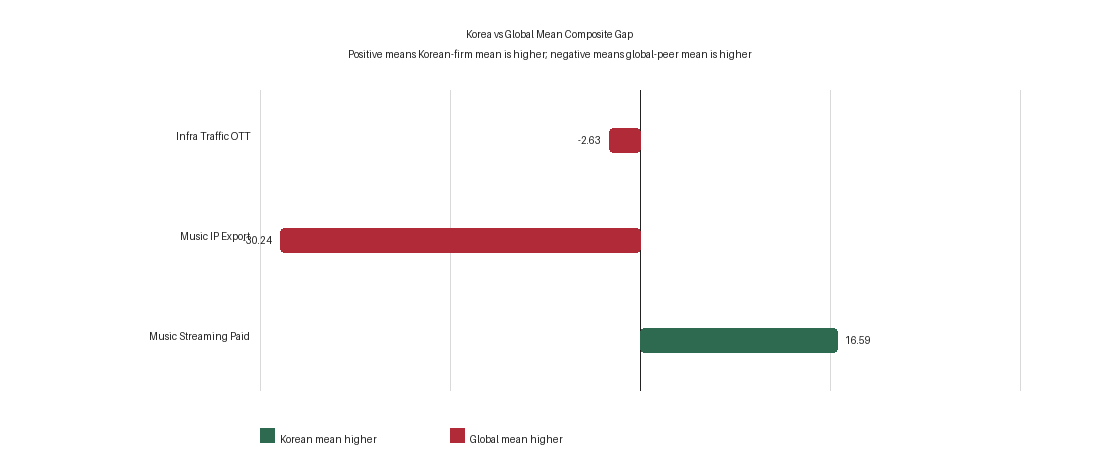
\includegraphics[width=0.88\textwidth]{outputs/figures/claim_strengthening/F_claim_korea_vs_global_gap.png}
\caption{한국 vs 글로벌 peer 평균 격차: 기존 직접 비교 참고도표}
\label{fig:claim_gap_main}
\end{figure}

표~\ref{tab:claim_peer_rank_appendix}는 선정된 비교군 안에서 협의 합성지표의 순위를 보여 준다. 인프라는 \texttt{kt}, 음악 IP 수출은 \texttt{warner\_music}, 음악 스트리밍은 \texttt{dreamus}가 가장 높다. 음악 스트리밍의 \texttt{kakao\_ent}는 적격 관측치가 없어 대체 평균으로 순위를 계산했다. 이 순위는 비교군 내부의 위치를 나타내며, 산업 전체의 평균 부담이나 한국시장 사례별 부담귀착 방향과는 구분한다. 사례별 방향점수는 표~\ref{tab:signed_korea_market_case_studies}에 제시한다.

\begin{table}[H]
\centering
\caption{비교군 내부 협의 합성지표 순위표}
\label{tab:claim_peer_rank_appendix}
\footnotesize
\setlength{\tabcolsep}{3pt}
\begin{tabular}{p{3.4cm}p{2.0cm}rrp{3.8cm}}
\toprule
\rowcolor{ReportTableHead}
비교 묶음 & 기업 & 점수 & 순위 & 비고 \\
\midrule
디지털 인프라 트래픽-OTT & \texttt{kt} & 51.806 & 1 & 비교군 평균 대비 +12.550 \\
디지털 인프라 트래픽-OTT & \texttt{netflix} & 39.255 & 2 & 글로벌 비교군 기준선 \\
디지털 인프라 트래픽-OTT & \texttt{lg\_uplus} & 33.528 & 3 & 비교군 평균 대비 -5.727 \\
디지털 인프라 트래픽-OTT & \texttt{sk\_telecom} & 24.555 & 4 & 비교군 평균 대비 -14.701 \\
음악 IP 수출 & \texttt{warner\_music} & 51.850 & 1 & 글로벌 비교군 기준선 \\
음악 IP 수출 & \texttt{jyp\_ent} & 30.710 & 2 & 비교군 평균 대비 -21.140 \\
음악 IP 수출 & \texttt{yg\_ent} & 12.500 & 3 & 비교군 평균 대비 -39.350 \\
음악 스트리밍 & \texttt{dreamus} & 50.000 & 1 & 비교군 평균 대비 +24.925 \\
음악 스트리밍 & \texttt{kakao\_ent} & 33.333 & 2 & fallback 평균 사용 \\
음악 스트리밍 & \texttt{spotify} & 25.075 & 3 & 글로벌 비교군 기준선 \\
\bottomrule
\end{tabular}

\vspace{0.3em}
{\par\raggedright\footnotesize 주: \texttt{kakao\_ent}는 \texttt{rank\_eligible} 관측치가 없어 \texttt{all\_row\_mean\_fallback}으로 순위를 계산했다. 이 대체값을 포함한 순위와 사례별 부담귀착 방향점수는 비교단위가 다르다. 후자는 표~\ref{tab:signed_korea_market_case_studies}에 제시한다.\par}
\end{table}

표~\ref{tab:claim_leave_one_peer_appendix}는 \texttt{netflix}, \texttt{warner\_music}, \texttt{spotify}를 하나씩 제외한 결과다. Netflix나 Warner Music을 제외해도 국내 부담이 높은 비교군의 존재는 유지된다. Spotify를 제외하면 이 초기 표본에서 유일하게 국내 부담이 높았던 음악 스트리밍 비교를 계산할 수 없게 된다. 따라서 이 표본만으로 산업 전체의 평균 부담 차이를 일반화할 수 없다. 이는 본문에서 복수 비교기업과 관측축을 사용해 산출한 확장 방향점수의 민감도 검정과 구분되는 결과다.

\begin{table}[H]
\centering
\caption{글로벌 비교군 하나씩 제외한 순차 제외 요약}
\label{tab:claim_leave_one_peer_appendix}
\footnotesize
\setlength{\tabcolsep}{3pt}
\resizebox{\textwidth}{!}{%
\begin{tabular}{p{2.2cm}cp{2.1cm}cp{5.9cm}}
\toprule
\rowcolor{ReportTableHead}
제외 비교군 & 남는 비교군 수 & 지지 방향 변화 & 부호 & 요약 \\
\midrule
\texttt{netflix} & 2 & 1 $\rightarrow$ 1 & 예 & 남는 두 비교군 모두 기존 격차 방향과 한국 내부 순위가 유지된다. \\
\texttt{warner\_music} & 2 & 1 $\rightarrow$ 1 & 예 & 남는 두 비교군 모두 기존 격차 방향과 한국 내부 순위가 유지된다. \\
\texttt{spotify} & 2 & 1 $\rightarrow$ 0 & 예 & 음악 스트리밍 비교가 비추정 상태가 되면서 지지 방향 비교군이 사라진다. \\
\bottomrule
\end{tabular}
}

\vspace{0.3em}
{\par\raggedright\footnotesize 주: 추정 가능한 비교군의 격차 부호는 유지된다. 다만 \texttt{spotify}를 제외하면 국내 부담이 높은 음악 스트리밍 비교를 계산할 수 없으므로, 이 초기 표본은 비교군 선택에 민감하다.\par}
\end{table}

그림~\ref{fig:claim_concentration_decomp_appendix}는 한국 음악 차트 대리지표에서 국내 상위 집중도와 글로벌 상위 집중도를 분해한 것이다. 직접 분해할 수 있는 음악 분야 두 묶음을 대상으로 한다. \texttt{KR music chart proxy market}은 차트 자료로 구성한 분석단위이므로, 이 비중을 동일 서비스의 이용자·매출 점유율로 해석하지 않는다.

\begin{figure}[H]
\centering
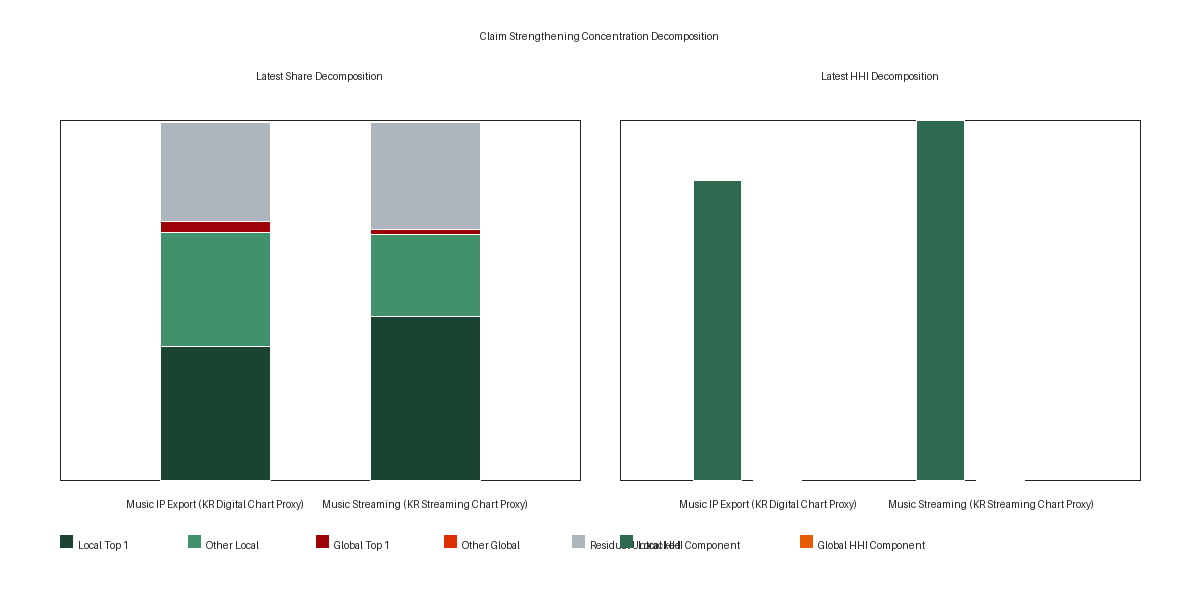
\includegraphics[width=0.88\textwidth]{outputs/figures/claim_strengthening/F_claim_concentration_decomposition.png}
\caption{한국 음악 차트 대리지표 시장의 집중도 분해}
\label{fig:claim_concentration_decomp_appendix}
\end{figure}

\noindent\begin{minipage}{0.93\textwidth}
\small
근거: 표~\ref{tab:claim_peer_rank_appendix}, 표~\ref{tab:claim_leave_one_peer_appendix}, 그림~\ref{fig:claim_concentration_decomp_appendix}.\\
\texttt{T\_claim\_peer\_rank.csv},\\
\texttt{T\_claim\_leave\_one\_peer\_}\\\texttt{out.csv},\\
\texttt{concentration\_decomposition\_}\\\texttt{table.csv},\\
\texttt{econ\_extension\_sensitivity\_}\\\texttt{pack.csv},\\
\texttt{legacy\_to\_econ\_crosswalk\_}\\\texttt{final.csv}.\\
재현 산출물 정리.\sourcefootnote{OpenDART, SEC EDGAR, Circle Chart, claim-strengthening processed outputs}
\end{minipage}

\section{변수 정의}
\subsection{표기 원칙}
아래 통합 변수 사전은 광의 설계 후보군과 후속 측정항목의 사전이다. 현재 결과의 코드형 변수 정의와 대체 측정은 본문의 실행 사양 및 다음 절의 실행 입력변수 사전을 적용한다. 같은 코드명을 쓰더라도 광의 설계 산식을 현재 결과의 계산식으로 대체하지 않는다. 각 후보항목은 ``관측값''과 ``가공값''을 분리하여 제시한다. ``관측값''은 공개자료에서 직접 수집 가능한 수치이고, ``가공값''은 관측값을 결합한 비율, 격차, 지수, 또는 시뮬레이션 입력값이다. 기대 부호는 구조적 불평등 심화 방향을 기준으로 표기한다.

\begin{landscape}
\subsection{I\_reg 변수 사전}
\tiny
\setlength{\tabcolsep}{1.0pt}
\begin{longtable}{@{}L{2.0cm}L{1.8cm}L{0.8cm}L{1.6cm}L{2.6cm}L{4.1cm}L{1.0cm}L{0.8cm}L{2.6cm}L{1.1cm}L{2.5cm}L{1.7cm}@{}}
\caption{I\_reg 광의 설계 후보 변수 사전} \\
\toprule
\rowcolor{ReportTableHead}
변수명 & 한글 변수명 & 유형 & 분야 & 정의 & 산식 & 단위 & 기대 부호 & 원천 데이터셋 & 결측 가능성 & 전처리 규칙 & 최종 사용 위치 \\
\midrule
\endfirsthead
\toprule
\rowcolor{ReportTableHead}
변수명 & 한글 변수명 & 유형 & 분야 & 정의 & 산식 & 단위 & 기대 부호 & 원천 데이터셋 & 결측 가능성 & 전처리 규칙 & 최종 사용 위치 \\
\midrule
\endhead
\WrapCell{reg\_lag\_\\months} & 규제 시차 개월수 & 가공값 & 전 분야 & 글로벌 플랫폼의 국내 진입 시점 대비 실효 규제 또는 최초 집행 개시 시점의 지연 길이 & \WrapCell{$(t^{\mathrm{glob}}_{\mathrm{enforce}}-$\\$t^{\mathrm{glob}}_{\mathrm{entry}})/30.4$} & 개월 & + & KCC 공식 공표자료, KCC OTT 영향분석, OpenDART/EDGAR & 중간 & 사건일을 월 단위로 정렬하고 음수값은 0으로 절단, 분기별 중앙값 집계 & $I_{\mathrm{reg}}$, 회귀 \\
\WrapCell{obligation\_\\count} & 실효규제의무 격차 건수 & 가공값 & 전 분야 & 국내 사업자에 적용되는 규제의무 수와 글로벌 비교군에 실효 집행된 의무 수의 차이 & \WrapCell{$\sum_k 1\{\text{domestic apply}\}$\\$-\sum_k 1\{\text{global enforce}\}$} & 건 & + & KCC 공식 공표자료, 사업보고서 리스크 공시 & 높음 & 의무 항목 목록을 고정 사전으로 정의하고 플랫폼별 적용 여부를 0/1로 부호화 & $I_{\mathrm{reg}}$ \\
\WrapCell{reporting\_\\burden\_\\days} & 절차부담일수 격차 & 가공값 & 전 분야 & 국내 사업자와 글로벌 비교군의 연간 신고·심의·자료제출·갱신 절차에 필요한 공식 소요일수 차이 & $\mathrm{days}_{\mathrm{dom}}-\mathrm{days}_{\mathrm{glob}}$ & 일 & + & KCC 공식 공표자료, 사업보고서 & 높음 & 공식 안내문의 소요일수를 합산하고 연 단위를 분기 단위로 1/4 배분 & $I_{\mathrm{reg}}$ \\
\WrapCell{compliance\_\\cost\_\\ratio} & 규제준수비용률 격차 & 가공값 & 전 분야 & 국내 사업자와 글로벌 비교군의 규제 준수 직접비용의 매출 대비 비율 차이 & \WrapCell{$(\text{compliance cost}/\text{revenue})_{\mathrm{dom}}-$\\$(\text{compliance cost}/\text{revenue})_{\mathrm{glob}}$} & \%p & + & \WrapCell{OpenDART, SEC EDGAR,\\사업보고서 주석} & 중간 & 비용 항목은 지급수수료·법무·심의·정책 대응 비용으로 일관 분류 & $I_{\mathrm{reg}}$, 회귀 \\
\WrapCell{network\_\\cost\_\\ratio} & 네트워크비용률 격차 & 가공값 & 디지털 인프라/음악 & 국내 사업자와 글로벌 비교군의 네트워크·전송·클라우드·CDN 비용의 매출 대비 비율 차이 & \WrapCell{$(\mathrm{net+cloud}/\mathrm{rev})_{\mathrm{dom}}-$\\$(\mathrm{net+cloud}/\mathrm{rev})_{\mathrm{glob}}$} & \%p & + & \WrapCell{OpenDART, SEC EDGAR,\\KCC 트래픽 자료,\\Cloudflare 후보} & 중간 & 공시 주석상 유사 항목을 통합하고 분기 평균으로 환산 & $I_{\mathrm{reg}}$, 시뮬레이터 \\
\WrapCell{effective\_\\tax\_\\rate\_gap} & 유효세율 격차 & 가공값 & 전 분야 & 국내 플랫폼 유효세율과 글로벌 비교군 유효세율의 차이 & $\mathrm{ETR}_{\mathrm{dom}}-\mathrm{ETR}_{\mathrm{glob}}$ & \%p & + & OpenDART, SEC EDGAR & 낮음 & ETR는 세전이익 대비 법인세비용으로 계산하고 음수 분모 표본은 제외 & $I_{\mathrm{reg}}$ \\
\WrapCell{infra\_\\dependency\_\\ratio} & 외부인프라 의존 격차 & 가공값 & 디지털 인프라 & 국내 사업자와 글로벌 비교군의 외부 클라우드·전송 인프라 지출의 서비스비용 대비 비율 차이 & \WrapCell{$(\mathrm{ext\ infra}/\mathrm{svc})_{\mathrm{dom}}-$\\$(\mathrm{ext\ infra}/\mathrm{svc})_{\mathrm{glob}}$} & \%p & + & \WrapCell{OpenDART, SEC EDGAR,\\OECD Broadband statistics} & 중간 & 통화 단위를 원화로 환산하고 분기 평균화, 글로벌 비교군은 동일 사업모형 기업군 중앙값 사용 & $I_{\mathrm{reg}}$, 회귀 \\
reg\_asym\_index & 규제비대칭지수 & 가공값 & 전 분야 & 다섯 개 제도 구성요소 부분지수를 합성한 규제 비대칭 복합지수 & $\frac{1}{5}\sum_{m \in M_{\mathrm{reg}}} C^m$ & 지수 & + & 상기 제도 변수 묶음 & 낮음 & 기준 사양에서는 구성요소 동일가중, 결측 시 관측 성분만으로 재정규화 & $I_{\mathrm{reg}}$ \\
\bottomrule
\end{longtable}
\normalsize
\end{landscape}

\begin{landscape}
\subsection{I\_risk 변수 사전}
\tiny
\setlength{\tabcolsep}{1.0pt}
\begin{longtable}{@{}L{2.0cm}L{1.8cm}L{0.8cm}L{1.7cm}L{2.7cm}L{3.9cm}L{1.0cm}L{0.8cm}L{2.7cm}L{1.1cm}L{2.5cm}L{1.7cm}@{}}
\caption{I\_risk 광의 설계 후보 변수 사전} \\
\toprule
\rowcolor{ReportTableHead}
변수명 & 한글 변수명 & 유형 & 분야 & 정의 & 산식 & 단위 & 기대 부호 & 원천 데이터셋 & 결측 가능성 & 전처리 규칙 & 최종 사용 위치 \\
\midrule
\endfirsthead
\toprule
\rowcolor{ReportTableHead}
변수명 & 한글 변수명 & 유형 & 분야 & 정의 & 산식 & 단위 & 기대 부호 & 원천 데이터셋 & 결측 가능성 & 전처리 규칙 & 최종 사용 위치 \\
\midrule
\endhead
\WrapCell{content\_\\investment\_\\ratio} & 콘텐츠투자비율 & 가공값 & 음악/웹툰 및 스토리 & 콘텐츠 확보, 제작, 선급금 등의 투자액이 매출에서 차지하는 비율 & \WrapCell{$\text{content investment}/$\\$\text{revenue}$} & \% & + & OpenDART, SEC EDGAR, KOCCA 음악산업백서 & 중간 & 제작·판권·콘텐츠 자산 항목을 통합하고 분기화 & $I_{\mathrm{risk}}$, 회귀 \\
\WrapCell{investment\_\\recovery\_\\ratio} & 제작비회수율 & 가공값 & 음악/웹툰 및 스토리 & 콘텐츠 관련 추정 매출이 투자액을 얼마나 회수하는지 나타내는 비율 & \WrapCell{$\text{estimated content revenue}/$\\$\text{content investment}$} & 배 & - & \WrapCell{KOCCA 웹툰산업 실태조사,\\KOCCA 음악산업백서,\\OpenDART} & 높음 & 공시 가능한 투자항목과 장르별 매출을 매칭, 극단치는 winsorize & $I_{\mathrm{risk}}$, 시뮬레이터 \\
\WrapCell{creator\_\\share\_\\ratio} & 창작자수익배분률 & 가공값 & 음악/웹툰 및 스토리 & 총 콘텐츠 매출 중 창작자 또는 권리자에게 귀속되는 비율 & \WrapCell{$\text{creator payout}/$\\$\text{gross content revenue}$} & \% & - & \WrapCell{KOCCA 웹툰산업 실태조사,\\KOCCA 음악산업백서} & 중간 & 설문·백서 기준치를 연도별 통일 기준으로 환산 & $I_{\mathrm{risk}}$ \\
\WrapCell{settlement\_\\delay\_\\days} & 정산지연일수 & 가공값 & 음악/웹툰 및 스토리 & 매출 발생 시점부터 정산 수취까지 평균 지연일수 & $\text{payment date}-\text{sale date}$ & 일 & + & KOCCA 웹툰산업 실태조사, KOCCA 산업 백서류 & 높음 & 응답분포의 중앙값 사용, 연 단위를 분기 단위로 환산 & $I_{\mathrm{risk}}$ \\
\WrapCell{funding\_\\cost\_\\spread} & 자금조달비용 스프레드 & 가공값 & 전 분야 & 국내 사업자 차입비용률과 글로벌 비교군 차입비용률의 차이 & \WrapCell{$(\text{interest expense}/\overline{\text{debt}})_{\mathrm{dom}}-$\\$(\text{interest expense}/\overline{\text{debt}})_{\mathrm{glob}}$} & \%p & + & OpenDART, SEC EDGAR & 중간 & 평균 차입금은 기초·기말 이자발생부채 평균으로 계산, 비교군은 동일 사업모형 중앙값 사용 & $I_{\mathrm{risk}}$, 회귀 \\
\WrapCell{ip\_assetization\_\\gap} & IP자산화결손 & 가공값 & 웹툰 및 스토리 & 글로벌 비교군 기준치 대비 국내 사업자의 IP 자산화 비율 결손 & \WrapCell{$\theta^{\mathrm{ip}}_{s,q}-$\\$(\text{IP intangible assets}/$\\$\text{total assets})_{\mathrm{dom}}$} & \%p & + & \WrapCell{OpenDART, SEC EDGAR,\\WIPO IP Statistics} & 중간 & 무형자산 주석에서 IP 관련 항목만 선별하고 기준치 $\theta^{\mathrm{ip}}$는 동일 연도 비교군 중앙값으로 계산 & $I_{\mathrm{risk}}$, 시뮬레이터 \\
\WrapCell{cashflow\_\\recovery\_\\ratio} & 현금흐름대비투자회수비율 & 가공값 & 전 분야 & 영업현금흐름이 콘텐츠 및 플랫폼 투자액을 얼마나 커버하는지 나타내는 비율 & \WrapCell{$\text{operating cash flow}/$\\$\text{content investment}$} & 배 & - & OpenDART, SEC EDGAR & 낮음 & 분모가 0인 경우 결측 처리, 1\%/99\% winsorize & $I_{\mathrm{risk}}$, 회귀 \\
\WrapCell{risk\_\\pressure\_\\index} & 리스크압력지수 & 가공값 & 전 분야 & 회수위험, 정산지연, IP 담보화 제약, 조달비용 스프레드, 배분률 결손을 통합한 복합지수 & $\frac{1}{5}\sum_{m \in M_{\mathrm{risk}}} C^m$ & 지수 & + & 상기 리스크 변수 묶음 & 낮음 & 기준 사양에서는 경제적 기준점 결손을 먼저 계산한 뒤 구성요소 동일가중으로 집계 & $I_{\mathrm{risk}}$ \\
\bottomrule
\end{longtable}
\normalsize
\end{landscape}

\begin{landscape}
\subsection{I\_market 변수 사전}
\tiny
\setlength{\tabcolsep}{1.0pt}
\begin{longtable}{@{}L{2.0cm}L{1.8cm}L{0.8cm}L{1.7cm}L{2.8cm}L{3.5cm}L{1.0cm}L{0.8cm}L{2.7cm}L{1.2cm}L{2.7cm}L{1.8cm}@{}}
\caption{I\_market 광의 설계 후보 변수 사전} \\
\toprule
\rowcolor{ReportTableHead}
변수명 & 한글 변수명 & 유형 & 분야 & 정의 & 산식 & 단위 & 기대 부호 & 원천 데이터셋 & 결측 가능성 & 전처리 규칙 & 최종 사용 위치 \\
\midrule
\endfirsthead
\toprule
\rowcolor{ReportTableHead}
변수명 & 한글 변수명 & 유형 & 분야 & 정의 & 산식 & 단위 & 기대 부호 & 원천 데이터셋 & 결측 가능성 & 전처리 규칙 & 최종 사용 위치 \\
\midrule
\endhead
\WrapCell{local\_platform\_\\share} & 로컬플랫폼점유율 & 관측값 & 전 분야 & 국내 사업자 플랫폼의 이용자, 이용시간 또는 매출 점유율 & \WrapCell{$\text{local metric}/$\\$\text{total market metric}$} & \% & - & KOCCA 콘텐츠 이용행태 조사, KISDI 미디어패널, OpenDART & 중간 & 부문별 분모를 통일하고 분기 평균으로 집계, 잠식속도 산출에는 전기 대비 변화율 사용 & $I_{\mathrm{market}}$, 회귀 \\
\WrapCell{cross\_market\_\\transfer\_\\index} & 시장간전이지수 & 가공값 & 음악/웹툰 및 스토리 & 지배 플랫폼의 인접시장 주목도 또는 점유율이 목표시장 점유율로 전환되는 정도 & $s_{\mathrm{target}}/a_{\mathrm{adjacent}}$ & 배 & + & Circle Chart, KISDI 미디어패널, NAVER DataLab API, YouTube API 후보 & 높음 & 음악 분야는 동영상-음원 전이, 타 분야는 인접 퍼널 주목도 자료로 대체하며 정의 불가능 시 NA 처리 & $I_{\mathrm{market}}$, 사건연구 \\
market\_hhi & 시장집중도 & 가공값 & 전 분야 & 시장 참여자 점유율 제곱합으로 계산한 집중도 & $\sum_j s_j^2$ & 지수 & + & KOCCA 조사, KCC 보고서, OpenDART & 중간 & 점유율을 0--1로 정규화 후 계산 & $I_{\mathrm{market}}$ \\
\WrapCell{concentration\_\\ratio\_\\top3} & 상위3사집중률 & 가공값 & 전 분야 & 상위 3개 사업자의 합산 점유율로 측정한 집중도 & $\sum_{i \in \mathrm{Top3}} s_i$ & \% & + & KOCCA 조사, KISDI 미디어패널, Circle Chart, KCC 보고서 & 중간 & 플랫폼 순위를 분기별로 재정렬하고 동일 분모 기준 적용 & $I_{\mathrm{market}}$ \\
\WrapCell{bundle\_\\leverage\_\\index} & 번들지배력지수 & 가공값 & 음악/OTT & 결합상품 또는 끼워팔기 노출이 독립 서비스 수요를 얼마나 대체하는지 나타내는 비율 & $D_{\mathrm{bundle}}/D_{\mathrm{single}}$ & 배 & + & NAVER DataLab API, KCC 공식 공표자료, KCC OTT 보고서 & 높음 & 검색지수와 공개 가입지표를 동일 기간 표준화 후 결합하고 출시 전후 기준 재계산 & $I_{\mathrm{market}}$, 사건연구 \\
\WrapCell{switching\_\\cost\_\\proxy} & 전환비용프록시 & 가공값 & 전 분야 & 지배 플랫폼 이용자 중 멀티호밍을 하지 않는 비율로 측정한 전환장벽 proxy & $1-\mathrm{multihoming\ rate}_{\mathrm{dominant}}$ & \% & + & KISDI 미디어패널, KOCCA 콘텐츠 이용행태 조사 & 중간 & 동일 플랫폼군 사용자를 기준으로 산출하고 표본가중치를 적용해 분기 평균화 & $I_{\mathrm{market}}$, 회귀 \\
\WrapCell{foreign\_\\dependency\_\\ratio} & 해외의존비율 & 가공값 & 전 분야/디지털 인프라 & 해외 플랫폼 트래픽 비중과 해외 인프라 의존도를 결합한 해외의존 지표 & $0.5T_{\mathrm{foreign}}+0.5F_{\mathrm{infra}}$ & \% & + & KCC 보고서, OpenDART, SEC EDGAR, ITU, Cloudflare 후보 & 중간 & 각 성분을 동일 분기 기준으로 정규화하고 결측 시 관측 성분만으로 평균화 & $I_{\mathrm{market}}$, 회귀 \\
\WrapCell{market\_\\transfer\_\\index} & 시장력전이지수 & 가공값 & 전 분야 & 전이, 집중, 락인, 해외의존, 로컬점유율 잠식속도를 통합한 복합지수 & $\frac{1}{5}\sum_{m \in M_{\mathrm{market}}} C^m$ & 지수 & + & 상기 시장 변수 묶음 & 낮음 & 기준 사양에서는 구성요소 동일가중, 사건연구형과 패널형 모두 동일 구성요소 사용 & $I_{\mathrm{market}}$ \\
\bottomrule
\end{longtable}
\normalsize
\end{landscape}

\begin{landscape}
\subsection{통제변수 및 시뮬레이터 입력값 사전}
\tiny
\setlength{\tabcolsep}{1.0pt}
\begin{longtable}{@{}L{2.0cm}L{1.8cm}L{0.8cm}L{1.7cm}L{2.8cm}L{3.5cm}L{1.0cm}L{0.8cm}L{2.7cm}L{1.2cm}L{2.7cm}L{1.8cm}@{}}
\caption{통제변수 및 시뮬레이터 입력값 사전} \\
\toprule
\rowcolor{ReportTableHead}
변수명 & 한글 변수명 & 유형 & 분야 & 정의 & 산식 & 단위 & 기대 부호 & 원천 데이터셋 & 결측 가능성 & 전처리 규칙 & 최종 사용 위치 \\
\midrule
\endfirsthead
\toprule
\rowcolor{ReportTableHead}
변수명 & 한글 변수명 & 유형 & 분야 & 정의 & 산식 & 단위 & 기대 부호 & 원천 데이터셋 & 결측 가능성 & 전처리 규칙 & 최종 사용 위치 \\
\midrule
\endhead
arpu\_proxy & 이용자당월지출 proxy & 가공값 & 전 분야 & 월평균 지출액을 유료 이용자 수로 나눈 이용자당 매출 proxy & $\text{monthly spending}/\text{paid users}$ & 원 & 통제 & KOCCA 콘텐츠 이용행태 조사, KISDI 미디어패널 & 중간 & 지출액을 월 기준으로 환산, 통화 단위 통일 & 회귀 통제, 시뮬레이터 \\
\WrapCell{paid\_\\subscription\_\\ratio} & 유료구독비율 & 가공값 & 전 분야 & 활성 이용자 중 유료 구독자의 비율 & $\text{paid users}/\text{active users}$ & \% & 통제 & KOCCA 콘텐츠 이용행태 조사, KCC 방송매체조사 & 중간 & 활성 이용자 정의를 조사 문항 기준으로 고정 & 회귀 통제 \\
\WrapCell{broadband\_\\price\_\\index} & 광대역가격지수 & 관측값 & 디지털 인프라 & 국제 비교 가능한 광대역 또는 데이터 접속 가격 수준 지표 & \text{official price index} & 지수 & + & OECD Broadband statistics, ITU DataHub & 낮음 & 기준연도 100으로 재기준화 & 회귀 통제, 국제 비교 \\
\WrapCell{mobile\_data\_\\usage\_\\per\_user} & 사용자당데이터이용량 & 가공값 & 디지털 인프라 & 가입자 1인당 월평균 데이터 사용량 & $\text{total mobile data}/\text{subscribers}$ & GB/월 & 통제 & KOSIS OpenAPI, ITU DataHub & 낮음 & 월 단위 표본을 분기 평균으로 집계 & 회귀 통제 \\
\WrapCell{collective\_\\bargaining\_\\premium} & 단체협상프리미엄 & 가공값 & 음악/웹툰 및 스토리 & 단체 협상 시 현재 대비 추가 확보 가능한 수익배분률 & $\text{negotiated share}-\text{current share}$ & \%p & - & KOCCA 실태조사, 공개 거래사례, OpenDART & 높음 & 기본 시나리오와 정책 시나리오를 분리 계산 & 시뮬레이터 \\
\WrapCell{securitization\_\\npv\_\\delta} & IP자산화 NPV 증분 & 가공값 & 웹툰 및 스토리 & IP 금융 자산화 이후의 순현재가치가 현재 가치보다 얼마나 증가하는지 나타내는 차이 & $\text{NPV}_{\mathrm{securitized}}-\text{NPV}_{\mathrm{current}}$ & 원 & - & OpenDART, WIPO IP Statistics, KOCCA 웹툰산업 실태조사 & 높음 & 할인율 가정값을 시나리오별 분리 저장, 0보다 작은 값 허용 & 시뮬레이터, 정책대안 \\
\bottomrule
\end{longtable}
\normalsize
\end{landscape}

\chapter{실행 입력변수 사전}
\begingroup
\footnotesize
\begin{itemize}[leftmargin=1.8em,itemsep=0.35em]
\item \(x^{\mathrm{tax}}\), \nolinkurl{effective_tax_rate_gap}: 법인세비용/양의 세전이익에서 비한국 비교군 기준을 뺀 유효세율 격차.
\item \(x^{\mathrm{net}}\), \nolinkurl{network_cost_ratio}: 서비스 직접 망비용률 또는 망·클라우드 비용/매출. 국내외 차감 전 비용률.
\item \(x^{\mathrm{infra}}\), \nolinkurl{infra_dependency_ratio}: 망비용률과 해외의존 대리지표의 곱.
\item \(x^{\mathrm{fund}}\), \nolinkurl{funding_cost_spread}: 이자비용/차입금 잔액에서 비한국 비교군 기준을 뺀 조달비용 격차.
\item \(x^{\mathrm{ip}}\), \nolinkurl{ip_assetization_gap}: 비한국 비교군 무형자산/매출 기준에서 해당 기업의 같은 비율을 뺀 대리 격차.
\item \(x^{\mathrm{inv}}\), \nolinkurl{investment_recovery_ratio}: 매출/콘텐츠 투자액. 재무값 부재 시 작품 역순위 평균의 대체 적용.
\item \(x^{\mathrm{cash}}\), \nolinkurl{cashflow_recovery_ratio}: 세전이익/콘텐츠 투자액. 재무값 부재 시 현지 IP 표식과 역순위 곱의 평균. 실제 영업현금흐름 비율과의 구별.
\item \(x^{\mathrm{transfer}}\), \nolinkurl{cross_market_transfer_index}: 음악의 번들 요금비율·해외의존·차트 점유 대리지표 결합값 또는 웹툰 번역 표식/순위 평균.
\item \(x^{\mathrm{foreign}}\), \nolinkurl{foreign_dependency_ratio}: 서비스 직접 관측 또는 국가-분기 해외의존 대리지표. 일부 국가에서 이용자 도달률의 대체 적용.
\item \(x^{\mathrm{outflow}}\), \nolinkurl{outflow_to_capex_ratio}: 서비스 직접값 또는 망·클라우드 비용/설비투자. 해외 지급액의 직접 관측비율과의 구별.
\item \(B\), \nolinkurl{bundle_leverage_index}: YouTube Music 단독 요금/YouTube 결합상품 요금. 현재 하위지수에서는 비활성인 후보·정책 변수.
\item \(x^{\mathrm{creator,proxy}}_a\), \nolinkurl{creator_share_ratio}: 웹툰 현지 IP 표식 평균의 창작자 배분 대체값. 현재 하위지수에서 비활성. 정책 기준값에서는 별도 보정된 배분률 상태변수.
\item \(\mathrm{Rev}\), \nolinkurl{revenue}: 매출액. 정책 계산의 기준매출은 보정 입력의 원화 명목액.
\item \(\mathrm{PTI},\mathrm{Tax}\): 세전이익과 법인세비용.
\item \(\mathrm{Int},\mathrm{Debt}\): 이자비용과 차입금 잔액. 기간비용과 잔액의 구별.
\item \(\mathrm{IA},\mathrm{CI}\): 무형자산 장부금액과 콘텐츠 투자액.
\item \(\mathrm{NC},\mathrm{Capex}\): 망·클라우드 비용과 설비투자액.
\item \(b^{\mathrm{tax}},b^{\mathrm{fund}},b^{\mathrm{ip}}\): 세율·조달비용률·무형자산/매출의 비한국 비교군 중앙값 기준.
\item \(P^{\mathrm{single}},P^{\mathrm{bundle}},H\): 단독상품 가격, 결합상품 가격, 차트 점유 대리지표.
\item \(a,r_a,L_a,U_a\): 작품 인덱스, 작품 노출순위, 현지 IP 표식, 번역 작품 표식.
\item \(x^{\mathrm{inv,proxy}}_a,x^{\mathrm{cash,proxy}}_a,x^{\mathrm{transfer,proxy}}_a\): 작품별 투자회수·현금회수·시장전이 대체값. \(\mathrm{proxy}\)는 대체 측정 표시.
\item \nolinkurl{local_platform_share}: 보정 입력의 국내 플랫폼 점유율. BND 매출 회복 계산용 상태변수.
\item \nolinkurl{market_revenue}: 관련 시장 총매출의 보정 명목 원화액.
\item \nolinkurl{traffic_cost_pressure}: 해외 트래픽 처리비용의 매출 대비 압력률. 정책 기준값에서는 해외의존도와 망비용률에 기초한 보정값.
\item \nolinkurl{content_investment}: 정책 기준선의 콘텐츠 투자액.
\item \nolinkurl{securitization_npv_delta}: IP 금융에 따른 순현재가치 증가 가능액의 시나리오 입력.
\item \nolinkurl{collective_bargaining_premium}: 협상에 따른 배분률 증가 가정값.
\item \nolinkurl{eligible_revenue}: 창작자 배분 개선의 적용대상 매출액.
\item \nolinkurl{reach}, \nolinkurl{creator}: 한국시장 규제 포착범위와 창작자 보호비용 귀착의 방향축 이름. CPII 원시 입력과 구별.
\end{itemize}
\endgroup


\section{집계·정규화·방향지표 기호}
\begingroup
\footnotesize
\begin{itemize}[leftmargin=1.8em,itemsep=0.35em]
\item \(s,\mathcal S\): 분야 인덱스와 세 분야 집합.
\item \(c,q,e=(s,c,q)\): 시장 국가, 분기, 분야-국가-분기 관측행.
\item \(i,f,h\): 기업 인덱스. \(h\)는 비교기업 합산 또는 제외축의 임시 인덱스. 한국시장 짝비교의 \(f\)는 해외 비교기업.
\item \(r=(d,f),d,\mathcal R\): 한국 기업 \(d\)와 해외 기업 \(f\)의 비교행 및 전체 비교행 집합.
\item \(j,k\): 입력변수 및 하위지수·방향축 인덱스.
\item \(t\): 회귀식의 시간 인덱스.
\item \(J_k,\mathcal J\): 활성 하위지수 변수집합과 10개 활성 변수의 합집합.
\item \(J,J_p\): 정책 상태벡터의 전체 성분 집합과 시나리오별 조정 성분 집합. \(\mathcal J\) 외 보조 상태변수 포함.
\item \(M_{k,s,c,q}\): 해당 셀에서 관측된 하위지수 \(k\)의 활성 변수집합.
\item \(C^k_{s,q},K_{s,q}\): 주 분석국가 중 하위지수 \(k\) 가용 국가집합과 분야-분기의 가용 하위지수 집합.
\item \(I^k_{s,c,q},I^k_{s,q},\mathrm{CPII}_{s,q}\): 국가별 하위지수, 국가 집계 후 하위지수, 최종 분야-분기 지수.
\item \(\mathrm{CPII}_{f,q},\mathrm{CPII}_{i,q},\mathrm{CPII}_{h,q}\): 시장 국가별 점수를 평균한 기업-분기 CPII.
\item \(Q_s,Q_f,Q_i^\cap\): 분야 가용 분기, 기업 가용 분기, 기업과 타 본국 비교군의 공통 가용 분기 집합.
\item \(\bar{\mathrm{CPII}}_s,\bar{\mathrm{CPII}}_f\): 가용 분기의 분야 평균과 기업 평균.
\item \(\mathcal P_i,\mathcal E_i,G_i^{\mathrm{common}}\): 본국이 다른 동분야 기업집합, 공통기간 비교기업-분기 집합, 그 비교군과의 평균 점수 차이.
\item \(x_{j,e},x_{j,s,c,q},x^\star_{j,e},u_{j,e},u^W_{j,e},\tilde x_{j,e}\): 원시값, 동일 원시값의 풀어쓴 표기, 방향 통일값, 로그변환값, 윈저화값, 정규화 점수. \(\tilde x_{j,s,c,q}\)와 동일한 마지막 점수 표기.
\item \(d_j,N_j\): 방향 부호와 변수별 기준표본 유효 관측 수.
\item \(\mathcal L_\pm,\operatorname{sgn},\log\): 부호보존 로그변환, 부호함수, 자연로그.
\item \(p,h_p,m,\eta,u_{j,(m)},Q_j(p)\) [분위수 식]: 분위수 확률, 보간 위치, 그 정수부, 소수부, 순서통계량, 선형 보간 분위수.
\item \(\lfloor\cdot\rfloor,\operatorname{rank}_{\mathrm{avg}}\): 내림 연산과 동순위 평균순위.
\item \(z,v,\mathcal U_j,L_j(v),U_j(v)\) [고정 기준점 식]: 평가할 원시값, 변환·윈저화값, 기준값 목록, 엄격히 작은 기준값 수, 작거나 같은 기준값 수.
\item \(\mathcal N_{j,\mathrm{base}},\mathcal N_{\mathrm{base}},\mathcal A\): 변수별 고정 정규화, 그 벡터별 적용, 결측 규칙을 포함한 동일가중 CPII 집계.
\item \(|A|,\#A\): 집합 원소 수. 수치에 대한 \(|u|\)는 절댓값.
\item \(\min,\max,\sum,(\cdot)_+,1\{\cdot\}\): 최솟값, 최댓값, 합산, 양의 부분, 조건 충족 시 1인 지시함수.
\item \(a_{r,k},m_{r,k}\): 비교행의 축별 방향값과 관측 여부 지시변수.
\item \(s^{\mathrm{reg\_domestic}}_r,s^{\mathrm{risk\_recovery}}_r,s^{\mathrm{market\_transfer}}_r\): 제도부담·위험회수·시장전이의 원천 방향점수.
\item \(s^{\mathrm{reach\_gap}}_r,s^{\mathrm{creator\_incidence}}_r\): 규제 포착범위·창작자 보호비용 귀착의 원천 방향점수.
\item \(K^{\mathrm{core}},K^{\mathrm{ext}}\): 핵심 3축 집합과 추가 2축을 포함한 확장 5축 집합.
\item \(S_r^{\mathrm{core}},S_r^{\mathrm{ext}},n_r^{\mathrm{core}},n_r^{\mathrm{ext}}\): 핵심·확장 관측축 평균과 각 관측축 수.
\item \(R_s,\bar S_s^{\mathrm{core}},\bar S_s^{\mathrm{ext}}\): 분야별 비교행 집합과 그 핵심·확장 점수 평균.
\item \(O_r,S_r^{(-h)},w_k,S_r^{\min}\): 관측 확장축 집합, 한 축 제외 평균, 축별 가중치, 가중치 허용구간 내 최저 평균.
\end{itemize}
\endgroup

\section{회귀식과 정책 시나리오 기호}
\begingroup
\footnotesize
\begin{itemize}[leftmargin=1.8em,itemsep=0.35em]
\item \(y_{i,t}\): 패널 회귀 또는 사건연구의 종속변수.
\item \(\alpha_i\): 단위 고정효과.
\item \(\tau_t\): 시점 고정효과.
\item \(\beta\): 채널변수 또는 통제변수 계수벡터.
\item \(z_{i,t}\): CPII 관련 채널변수 또는 통제변수 벡터.
\item \(\varepsilon_{i,t}\): 회귀식 오차항.
\item \(T_i\): 단위 \(i\)의 사건시점.
\item \(\gamma_{\ell}\): 사건연구 상대시점 \(\ell\)의 효과계수.
\item \(z^{\mathrm{base}}_{s,q}\): 기준선 상태벡터.
\item \(z^{\mathrm{base}}_{j,s,q}\): 기준선 상태벡터의 \(j\)번째 성분.
\item \(z^{(p)}_{s,q}\): 정책 시나리오 \(p\) 적용 후 상태벡터.
\item \(z^{(p)}_{j,s,q}\): 정책 시나리오 \(p\) 적용 후 \(j\)번째 상태성분.
\item \(\Phi^{(p)}_{s,q}\): 기준선 상태벡터를 정책 후 상태벡터로 보내는 시나리오 사상.
\item \(\vartheta^{(p)}\): 정책 시나리오 \(p\)의 정책강도 및 전달계수 벡터.
\item \(J_p\): 정책 시나리오 \(p\)가 직접 조정하는 목표 변수 집합.
\item \(g^{(p)}_{j,s,q}\): 정책 시나리오 \(p\)의 성분별 조정 함수.
\item \(\Delta z^{(p)}_{j,s,q}\): 정책 시나리오 \(p\)에 따른 상태변수 변화량.
\item \(\tilde{x}^{(p)}_{j,s,q}\): 시나리오 입력의 고정 기준점 정규화 점수.
\item \(\mathcal G_p\): 시나리오 \(p\)의 계산 가능한 분야-분기 셀 집합.
\item \(\mathrm{CPII}_{\mathrm{base}}\): 기준선 CPII 총지수.
\item \(\mathrm{CPII}_{\mathrm{scenario}}\): 시나리오 적용 후 CPII 총지수.
\item \(\mathrm{CPII}^{\mathrm{base}}_{s,q}\): 분야-분기 기준선 CPII.
\item \(\mathrm{CPII}^{(p)}_{s,q}\): 분야-분기 시나리오 \(p\) 적용 후 CPII.
\item \(\Delta \mathrm{CPII}\): 기존 기준점수에서 시나리오 점수를 뺀 차이. 기준값 재구성 차이 포함.
\item \(\overline{\Delta \mathrm{CPII}}^{(p)}\): 시나리오 \(p\)의 평균 기존 점수 변화량.
\item \(\rho^{\mathrm{bundle}}_{s,q}\): BND 시나리오의 번들 제한 강도계수.
\item \(\eta^{\mathrm{transfer}}_{s,q}\): BND 시나리오의 시장전이 전달계수.
\item \(\eta^{\mathrm{share}}_{s,q}\): BND 시나리오의 점유율 회복 전달계수.
\item \(B_{s,q}\) [BND]: \nolinkurl{bundle_leverage_index}\(_{s,q}\)의 축약 상태변수.
\item \(T_{s,q}\) [BND]: \nolinkurl{cross_market_transfer_index}\(_{s,q}\)의 축약 상태변수.
\item \(L_{s,q}\) [BND]: \nolinkurl{local_platform_share}\(_{s,q}\)의 축약 상태변수.
\item \(M_{s,q}\) [BND]: \nolinkurl{market_revenue}\(_{s,q}\)의 축약 상태변수.
\item \(B^{(\mathrm{BND})}_{s,q}\): BND 적용 후 번들 강도.
\item \(T^{(\mathrm{BND})}_{s,q}\): BND 적용 후 시장전이 강도.
\item \(L^{(\mathrm{BND})}_{s,q}\): BND 적용 후 로컬 점유율.
\item \(RR^{(\mathrm{BND})}_{s,q}\): BND 적용 후 점유율 회복의 매출 환산액.
\item \(\phi^{\mathrm{recover}}_{s,q}\): NET 시나리오의 비용 회수율.
\item \(\psi^{\mathrm{capex}}_{s,q}\): NET 시나리오의 회수비용 국내 투자 전환율.
\item \(\kappa^{\mathrm{replace}}_{s,q}\): NET 시나리오의 해외 인프라 국내 대체율.
\item \(C_{s,q}\) [NET]: \nolinkurl{traffic_cost_pressure}\(_{s,q}\)의 축약 상태변수.
\item \(N_{s,q}\) [NET]: \nolinkurl{network_cost_ratio}\(_{s,q}\)의 축약 상태변수.
\item \(F_{s,q}\) [NET]: \nolinkurl{foreign_dependency_ratio}\(_{s,q}\)의 축약 상태변수.
\item \(O_{s,q}\) [NET]: \nolinkurl{outflow_to_capex_ratio}\(_{s,q}\)의 축약 상태변수.
\item \(R_{s,q}\) [NET]: \nolinkurl{revenue}\(_{s,q}\)의 축약 상태변수.
\item \(\mathrm{RecoveredCost}^{(\mathrm{NET})}_{s,q}\): NET 적용 후 회수 가능한 비용액.
\item \(\mathrm{DomesticCapexGain}^{(\mathrm{NET})}_{s,q}\): NET 적용 후 국내 설비투자 증가액.
\item \(N^{(\mathrm{NET})}_{s,q}\): NET 적용 후 망비용률.
\item \(F^{(\mathrm{NET})}_{s,q}\): NET 적용 후 해외의존비율.
\item \(O^{(\mathrm{NET})}_{s,q}\): NET 적용 후 해외유출 대비 설비투자 압박률.
\item \(\alpha^{\mathrm{ip}}_{s,q}\): IPF 시나리오의 자산화 채택률.
\item \(\lambda^{\mathrm{advance}}_{s,q}\): IPF 시나리오의 자산가치 대비 선급조달 비율.
\item \(\eta^{\mathrm{funding}}_{s,q}\): IPF 시나리오의 조달금리 개선 전달계수.
\item \(\eta^{\mathrm{recovery}}_{s,q}\): IPF 시나리오의 회수율 개선 전달계수.
\item \(S_{s,q}\) [IPF]: \nolinkurl{securitization_npv_delta}\(_{s,q}\)의 축약 상태변수.
\item \(A_{s,q}\) [IPF]: \nolinkurl{ip_assetization_gap}\(_{s,q}\)의 축약 상태변수.
\item \(G_{s,q}\) [IPF]: \nolinkurl{funding_cost_spread}\(_{s,q}\)의 축약 상태변수.
\item \(I_{s,q}\) [IPF]: \nolinkurl{investment_recovery_ratio}\(_{s,q}\)의 축약 상태변수.
\item \(C_{s,q}\) [IPF]: \nolinkurl{content_investment}\(_{s,q}\)의 축약 상태변수.
\item \(\mathrm{NPVGain}^{(\mathrm{IPF})}_{s,q}\): IPF 적용 후 추가 순현재가치.
\item \(\mathrm{FinanceCapacity}^{(\mathrm{IPF})}_{s,q}\): IPF 적용 후 선급조달 가능액.
\item \(A^{(\mathrm{IPF})}_{s,q}\): IPF 적용 후 IP 자산화 결손.
\item \(G^{(\mathrm{IPF})}_{s,q}\): IPF 적용 후 자금조달 스프레드.
\item \(I^{(\mathrm{IPF})}_{s,q}\): IPF 적용 후 투자 회수율.
\item \(\theta^{\mathrm{bargain}}_{s,q}\): CBA 시나리오의 협상 참여율 또는 적용 범위 계수.
\item \(\eta^{\mathrm{cash}}_{s,q}\): CBA 시나리오의 현금회수율 개선 전달계수.
\item \(R^{\mathrm{cr}}_{s,q}\): \nolinkurl{creator_share_ratio}\(_{s,q}\)의 축약 상태변수.
\item \(K_{s,q}\): \nolinkurl{cashflow_recovery_ratio}\(_{s,q}\)의 축약 상태변수.
\item \(P_{s,q}\): \nolinkurl{collective_bargaining_premium}\(_{s,q}\)의 축약 상태변수.
\item \(E_{s,q}\): \nolinkurl{eligible_revenue}\(_{s,q}\)의 축약 상태변수.
\item \(\Delta R^{\mathrm{cr},(\mathrm{CBA})}_{s,q}\): CBA 적용 후 창작자 배분률 증분.
\item \(\left(R^{\mathrm{cr}}\right)^{(\mathrm{CBA})}_{s,q}\): CBA 적용 후 창작자 배분률.
\item \(\mathrm{CreatorIncomeGain}^{(\mathrm{CBA})}_{s,q}\): CBA 적용 후 창작자 소득 증가액.
\item \(K^{(\mathrm{CBA})}_{s,q}\): CBA 적용 후 현금회수율.
\item \(\mathcal T,D^\ell_{i,t}\): 사건 노출단위 집합과 노출단위의 상대시점 지시변수.
\item \(\mathcal L,\ell=-1\): 사건 상대시점 집합과 회귀의 제외 기준시점.
\item \(\beta^\top z_{i,t}\): 계수벡터와 설명변수 벡터의 내적. \(\top\)는 전치 연산.
\item \(\mathrm{CPII}^{(0)}_{s,q}\): 재구성 입력벡터의 무변경 재계산 점수.
\item \(b^{\mathrm{rebase}}_{s,q}\): 기존 기준점수와 무변경 재계산 점수의 차이.
\item \(D^{(p)}_{s,q}\): 동일 재구성 입력 대비 시나리오 적용의 기계적 점수 감소량.
\item \(\Delta\mathrm{CPII}^{(p)}_{s,q}\): \(b^{\mathrm{rebase}}_{s,q}+D^{(p)}_{s,q}\)인 기존 변화량.
\item \(\delta^{\mathrm{eff}}_{s,q},\mathrm{CreatorIncomeGain}^{*}_{s,q}\): 배분률 상한을 반영한 유효 증분과 일관된 창작자 소득증분. 별표는 상한 일관성 수정식의 표시.
\item \(\Pi\), \nolinkurl{policy_priority_score}: 기존 정책 우선순위 점수. 0.55·0.15·0.10·0.10·0.10의 사전 가중합.
\item \(RR,DC,NG,CG\): 우선순위 식의 매출 회복액, 국내 설비투자 증가액, 추가 순현재가치, 창작자 소득증분. 시나리오별 원래 산출변수의 축약 표기.
\item \(M,R,C^{\mathrm{IPF}},E\): 우선순위 식의 시장매출, 기준매출, 콘텐츠 투자액, 적용대상 매출. 원 단위 분모.
\item \(A^{(p)}_{s,q}\): NET의 동일 셀 점수 감소량에서 비교정책 \(p\)의 감소량을 뺀 상대 우위.
\item \(\mathcal V,\nu\): 민감도 배율 집합 \(\{0.8,1.0,1.2\}\)과 그 원소.
\item \(\Delta\mathrm{CPII}^{(p,\nu)}_{s,q}\): 시나리오 \(p\)의 계수벡터에 배율 \(\nu\)와 허용범위 제한을 적용한 기존 점수 변화량.
\item \(A^{(p),\mathrm{adv}}_{s,q}\): NET의 최소 변화량과 비교정책의 최대 변화량 사이 차이.
\item \(\varepsilon=10^{-9}\): 정책 비율식의 영분모 방지용 양수.
\item \(\mathbb R,\mathcal Z_J,\mathrm{NA}\): 실수 집합, 결측 표식을 포함한 성분집합 \(J\)의 상태공간, 결측 표식.
\end{itemize}
\endgroup

\chapter{CPII 기업 비교기 v2}
\label{app:cpii_comparator_v2_method}
\label{app:comparator-v2}
\subsection*{비교 대상과 입력 조건}
\textbf{CPII 기업 비교기는 같은 산업·서비스·시장·분기의 기업별 부담을 동일한 기준분포에 놓고 비교하는 입력형 계산 도구.} 회사명 검색이나 외부자료 자동 수집 기능이 아니라, 사용자가 구성한 10개 입력변수의 정규화·합산·차이 분해 기능. v2의 변경 범위는 입력 검증과 결과 표시의 보강이며, v1의 활성 변수·방향·가중치·고정 기준분포는 유지.

\begin{itemize}[leftmargin=1.8em,itemsep=0.3em]
\item 관측단위: 기업-서비스-시장-분기. 비교집단의 식별 필드는 \nolinkurl{sector}, \nolinkurl{service_scope}, \nolinkurl{focal_market}, \nolinkurl{reporting_period}, \nolinkurl{benchmark_id}. 다섯 필드의 대소문자까지 일치하는 관측끼리의 비교.
\item 필수 입력: 규제 3개, 위험 4개, 시장 3개의 활성 변수 전부. 빈 셀은 실제 관측값 0과 구별하며, 불완전 입력의 순위·점수차 산출 차단. 과거 결과의 가용항목 평균과 달리 모든 비교기업에 동일한 10개 성분을 요구하는 완전입력 사양.
\item 입력 단위: 비율의 1\%는 \(0.01\), 배수의 3배는 \(3\). 세율·조달비용의 격차는 기업값에서 공통 기준값을 차감하고, IP 자산화 결손은 공통 무형자산/매출 기준에서 기업값을 차감하는 방향.
\item 출처 기록: 변수별 원천, 기준일, 산식, 직접값·가공값·대리값 구분. \nolinkurl{company_exposure_factor}는 시장공통값에 이미 적용한 기업별 노출조정의 기록이며, 계산기가 입력변수에 다시 곱하는 계수는 아님.
\item 등록 상태: 동봉된 \nolinkurl{BM-DIGITAL-CONTENT-2025Q4}는 합성 예시 전용 기준. 실제 기업 적용의 선행조건은 분야·분기별 실제 비교군, 격차 산식, 출처 해시의 등록과 계산파일 재생성. 합성 표식을 실제 기업에 붙여 입력 검증을 우회하는 사용의 배제.
\end{itemize}

\subsection*{고정 정규화와 점수차 분해}
기업 \(a\)의 변수 \(j\) 원값을 \(x_{j,a}\), 부담방향 부호를 \(d_j\), 변환함수를 \(T_j\)로 표시. 투자회수율과 세전이익 회수 대리값에 \(d_j=-1\), 나머지 활성 변수에 \(d_j=1\) 적용. 해외의존비율에는 항등변환, 나머지 9개에는 부호보존 로그변환 적용.
\[
T_j(z)=
\begin{cases}
z,&j=\mathrm{foreign},\\
\operatorname{sgn}(z)\log(1+|z|),&\text{그 밖의 활성 변수},
\end{cases}
\qquad
w_{j,a}=\min\{u_j,\max\{\ell_j,T_j(d_jx_{j,a})\}\}.
\]
\(\ell_j,u_j\)는 분야-국가-분기 결합 기준표본의 변환값에서 선형보간으로 산출한 1\%·99\% 분위수. 이 경계와 변수별 기준표본은 비교기업을 추가하거나 삭제해도 불변. \(n_j\)개의 고정 윈저화 기준값을 \(w^0_{j,r}\)로 표시할 때 적용하는 순위식은 다음과 같음.
\[
L_j(w)=\sum_{r=1}^{n_j}\mathbf1\{w^0_{j,r}<w\},\qquad
U_j(w)=\sum_{r=1}^{n_j}\mathbf1\{w^0_{j,r}\leq w\},
\]
\[
S_{j,a}=\frac{L_j(w_{j,a})+U_j(w_{j,a})-1}{2(n_j-1)},
\qquad
I^{k,\mathrm{cmp}}_a=\frac{100}{m_k}\sum_{j\in J_k}S_{j,a},
\qquad
C_a=\frac13\sum_k I^{k,\mathrm{cmp}}_a.
\]
동일 기준값에는 평균순위를 부여하고, 기준값 사이의 새 입력에는 위 계수식으로 위치를 부여하는 방식. 연속적인 비용률 변화가 언제나 연속적인 점수 변화로 이어지지는 않으며, 같은 순위 구간이나 윈저화 경계 밖의 서로 다른 원값에 같은 점수의 부여 가능성.

\begin{itemize}[leftmargin=1.8em,itemsep=0.3em]
\item \(j,a,b,r,z,w\): 변수, 두 비교기업, 기준관측의 인덱스, 변환 전 실수 인수, 윈저화 후 위치 인수.
\item \(x_{j,a},d_j,T_j,w_{j,a},\ell_j,u_j,w^0_{j,r},n_j\): 기업 원값, 방향 부호, 변환함수, 기업 윈저화 값, 하단·상단 경계, 고정 기준값, 변수별 기준관측 수.
\item \(L_j,U_j,\mathbf1\): 기준값 미만·이하의 누적 개수와 조건 성립 시 1인 지시함수. \(\operatorname{sgn}\)은 부호함수.
\item \(J_k,m_k,k\): 하위지수별 활성 변수 집합, 그 원소 수, 규제·위험·시장 하위지수 인덱스. \((m_{\mathrm{reg}},m_{\mathrm{risk}},m_{\mathrm{market}})=(3,4,3)\).
\item \(S_{j,a},I^{k,\mathrm{cmp}}_a,C_a\): 0--1 변수별 기준분포 위치, 0--100 비교기 하위지수, 0--100 비교기 CPII. 위첨자 \(\mathrm{cmp}\)는 비교기 사양의 표시.
\end{itemize}

\[
\Delta^{\mathrm{cmp}}_{ab}=C_a-C_b
=\sum_k\sum_{j\in J_k}c_{j,ab},
\qquad
c_{j,ab}=\frac{100}{3m_k}(S_{j,a}-S_{j,b}),\quad j\in J_k.
\]
\(\Delta^{\mathrm{cmp}}_{ab}\)는 A에서 B를 뺀 점수차, \(c_{j,ab}\)는 해당 변수의 점수 기여도. 규제·시장 변수 각각의 유효가중치는 \(1/9\), 위험 변수 각각은 \(1/12\). \textbf{양의 점수차는 A의 부담지수가 B보다 높다는 뜻이며, 개선의 뜻은 아님.} 반면 같은 기업의 개선량을 개선 전 점수에서 개선 후 점수를 뺀 값으로 정의하면 양수는 부담 감소의 뜻. 서로 다른 차감 순서의 구별.

\subsection*{합성 예시와 경제적 해석}
\begin{table}[H]
\centering
\small
\caption{비교기 합성 예시의 점수와 하위지수 기여도}
\begin{tabular}{lrrrr}
\toprule
지표 & 가온 콘텐츠(A) & 누리 미디어(B) & A--B & 총점차 기여 \\
\midrule
규제 하위지수 & 12.738 & 5.086 & 7.652 & 2.551 \\
위험 하위지수 & 73.358 & 65.062 & 8.296 & 2.765 \\
시장 하위지수 & 33.591 & 26.504 & 7.087 & 2.362 \\
CPII & 39.896 & 32.217 & 7.678 & 7.678 \\
\bottomrule
\end{tabular}
\par\smallskip
\begin{minipage}{0.96\linewidth}\footnotesize
실제 기업에 관한 관측·추정이 아닌 네 개 합성 예시 중 두 기업의 계산값. 하위지수 점수차의 3분의 1이 총점차 기여도이며, 반올림 전 값에 기초한 합계 검증.
\end{minipage}
\end{table}

이 예시의 \(7.678\)점은 세 경로 모두에서 A의 정규화 부담이 더 높다는 신호. 소비자 피해율 7.678\%, 위법 확률 7.678\%, 기업분포상의 백분위 차이와는 구별. 일반적으로 총점차가 양수여도 개별 변수 기여도는 음수일 수 있으므로, 총점 다음에 하위지수와 변수별 양·음 기여도의 확인 필요.

화폐금액은 점수차가 아니라 원단위 차이와 비교 가능한 경제적 노출액의 결합. 예를 들어 망비용률을 \(n_a,n_b\), 같은 기간·통화·가격기준의 매출액을 \(R_a,R_b\)로 놓으면 공통규모 비용 상당액은 다음과 같음.
\[
\bar R_{ab}=\frac{R_a+R_b}{2},\qquad
E^{\mathrm{net}}_{ab}=(n_a-n_b)\bar R_{ab}.
\]
\(\bar R_{ab}\)는 두 매출액의 산술평균, \(E^{\mathrm{net}}_{ab}\)는 공통 매출규모를 적용한 망비용 차이 상당액. 합성 예시의 비용률 \(0.180\)과 \(0.105\)에 공통 매출규모 1조원을 가정하면 \(0.075\times1\text{조원}=750\text{억원}\). 7.678 CPII점 전체의 금액환산이나 실제 손해액이 아닌, 한 채널의 조건부 회계 상당액.

인프라 결합값·해외의존도·비용/설비투자 비율의 별도 화폐환산은 비활성. 같은 비용을 공유하는 변수별 금액의 자동합산 금지. 조달비용의 기간환산은 입력 금리의 연율·분기율과 노출기간의 정합성을 전제로 하며, 이미 분기화된 비율에 분기계수를 다시 곱하는 중복 조정의 배제. 입력·노출액의 하한·기준·상한은 확률구간이 아닌 결정론적 민감도 가정.

\subsection*{v2 변경사항과 사용 순서}
\begin{itemize}[leftmargin=1.8em,itemsep=0.3em]
\item 인프라 관계식 검사 수정: v1의 열 순서 오인을 제거하고 변수명에 따라 망비용률·해외의존도·인프라 결합값의 위치를 식별. 점수 계산의 변경이 아니라 잘못된 관계식 경고의 수정.
\item 원본 예시 검증의 분리: 원래 관측 ID와 10개 값이 모두 같은 경우에만 고정 기대점수와 대조. 정상적인 예시 입력 변경은 새로운 계산으로 허용하고, 원본 예시 대조 대상에서 제외.
\item 입력조건의 명확화: 실제 달력에 존재하는 2000--2100년의 출처일, 영문 대문자·숫자·하이픈·밑줄·마침표로 구성된 1--64자 관측 ID, 지정된 분류값, 비교집단의 공백과 대소문자 검사. 임의의 한국어 회사명과 제한된 관측 ID의 구별.
\item 결과 보호: 입력 검증 실패 시 해당 기업의 비교화면 점수·짝비교 차이·기여도·금액·민감도 표시 차단. 비교집단이 다르면 전체 순위 대신 집단별 순위와 비교불가 표시.
\item 사용 순서: \nolinkurl{01_INPUT_COMPANIES}에 기업 입력, \nolinkurl{07_INPUT_PROVENANCE}에 변수별 근거 기록, 필요 시 \nolinkurl{02_INPUT_ECON_BASES}에 경제 노출액 입력, \nolinkurl{03_COMPARE_2}에서 두 기업의 점수·기여도 확인, \nolinkurl{04_COMPARE_N}에서 집단별 순위 확인, \nolinkurl{06_SENSITIVITY}와 \nolinkurl{99_QA_AUDIT}에서 민감도·검증 상태 확인.
\item 수용 한도: 기업 100개, 화면상의 짝비교 행렬 30개. 더 큰 집합의 비교 및 입력변수별 범위 민감도는 동봉 Python 엔진의 별도 실행. Excel 민감도 화면은 가중치·저지원 제외·중복채널 축소의 네 가지 사양 비교.
\end{itemize}

활성 10개 변수를 동시에 관측한 기준행은 전체 159행 중 2행이며, 시장간 전이와 해외의존의 저지원 변수 가중치는 합계 \(2/9=22.22\%\). 따라서 v2의 지위는 연구용 베타이며, 입력 검증 개선을 기준표본 확대나 새로운 인과적 식별로 해석하는 것은 부적절. 비용회수·투자회수·시장전이 경로를 분리하여 비교하고 반대 방향의 기여도까지 드러내는 것이 이 도구의 실질적 용도. 기존 실증 결과의 기업 평균, 한국시장 방향점수, 정책 시나리오 감소량을 합성 예시의 점수로 대체하는 사용의 배제.


% Source-only appendix candidate. Do not compile without the author's instruction.
% Based on the delivered CPII_Comparator_v2 workbook, inspected 2026-10-26.
\chapter{스프레드시트 시뮬레이터 사용 설명서}
\label{app:simulator-manual}

이 부록은 동봉한 \nolinkurl{CPII_Company_Comparator.xlsx}의 실제 화면을 기준으로 입력, 비교, 점검, 보관 절차를 설명한다. 대상 파일은 배포 폴더 \nolinkurl{outputs/client_delivery/CPII_Comparator_v2/}에 있으며, 파일 버전은 \nolinkurl{CPII_COMPARATOR_XLSX_V2.0.0}이다. 지수 산식과 해석은 부록~\ref{app:cpii_comparator_v2_method}를 참조하고, 여기서는 사용자가 어느 시트의 어떤 셀을 다루어야 하는지에 집중한다.

\begin{ReportCallout}
\textbf{처음 사용할 때는 동봉 예시로 계산 흐름부터 확인한다.} 비교기는 기업별 10개 변수를 받아 점수와 차이를 계산한다. 현재 등록된 비교기준 \nolinkurl{BM-DIGITAL-CONTENT-2025Q4}는 합성 예시용이다. 멜론과 스포티파이의 실제 자료를 적용하려면 서비스·시장·기간에 맞는 비교군, 변수 산식, 원천자료 해시를 등록하고 통합문서를 재생성해야 한다. 회사명만 바꾸어 기존 예시를 실제 기업의 결과로 제시해서는 안 된다.
\end{ReportCallout}

\section{빠른 시작: 열기에서 결과 확인까지}

\begin{enumerate}[leftmargin=1.8em,itemsep=0.45em]
\item 원본 파일을 보관하고, 날짜와 분석 목적을 붙인 작업 사본을 만든다. 예를 들어 \nolinkurl{CPII_Comparator_20261026_working.xlsx}로 저장한다. Excel의 계산 옵션은 자동으로 설정한다.
\item \nolinkurl{00_README}에서 버전과 입력 한도를 확인한다. 기본 예시는 \nolinkurl{01_INPUT_COMPANIES}의 7--10행에 들어 있다.
\item \nolinkurl{03_COMPARE_2}의 B4에서 \texttt{SYN-A}, B5에서 \texttt{SYN-B}를 선택한다. A14에 ``비교 가능''이 표시되는지 확인한다.
\item 같은 시트의 B8:D11에서 총점과 하위지수를 읽고, H17:H26에서 변수별 기여도를 확인한다. H28의 기여도 합계가 D8의 총점차와 일치하면 I28에 \texttt{PASS}가 표시된다.
\item \nolinkurl{06_SENSITIVITY}에서 사양을 바꿔도 차이의 방향이 유지되는지 살핀다. \nolinkurl{99_QA_AUDIT}에서 입력 오류와 합계 검증 상태를 확인한 뒤 결과를 저장한다.
\end{enumerate}

파란 입력 셀과 회사 선택 셀만 수정하는 것을 원칙으로 한다. 배포본에는 시트 보호가 설정되어 있지 않아 계산식도 덮어쓸 수 있다. 따라서 수식 영역을 직접 고치기보다 입력값을 수정하고 결과가 바뀌는지 확인한다. 원본 복사본은 수식 손상이나 입력 착오가 생겼을 때 되돌아갈 기준이 된다.

\clearpage
\section{시트 구성과 작업 범위}

\begin{longtable}{@{}L{4.0cm}L{3.1cm}L{7.6cm}@{}}
\caption{실제 배포 통합문서의 시트와 사용 위치}\label{tab:simulator-sheet-map}\\
\toprule
\rowcolor{ReportTableHead}
시트 & 작업 위치 & 용도 \\
\midrule
\endfirsthead
\toprule
\rowcolor{ReportTableHead}
시트 & 작업 위치 & 용도 \\
\midrule
\endhead
\bottomrule
\endfoot
\nolinkurl{00_README} & 읽기 전용으로 사용 & 빠른 시작, 버전, 점수의 의미, 입력 한도. \\
\nolinkurl{01_INPUT_COMPANIES} & A7:AC106 입력; AD열 점검 & 기업·서비스·시장·분기 정보와 활성 변수 10개. 최대 100개 관측. \\
\nolinkurl{02_INPUT_ECON_BASES} & A7:Z106 입력; AA열 점검 & 채널별 금액을 해석할 때 필요한 경제적 노출액과 가정. \\
\nolinkurl{03_COMPARE_2} & B4, B5 선택 & 두 기업의 총점, 하위지수, 변수별 점수차 기여도. \\
\nolinkurl{04_COMPARE_N} & A7:G106; J7:AM36 확인 & 비교집단별 순위와 최대 30개 관측의 짝비교 행렬. \\
\nolinkurl{05_ECON_INTERPRET} & 8--17행 확인 & 원값 차이와 노출액을 결합한 채널별 상당액·시나리오 금액. \\
\nolinkurl{06_SENSITIVITY} & A8:E11, B14:B18 확인 & 기본 사양과 세 가지 대체 사양의 점수차 비교. \\
\nolinkurl{07_INPUT_PROVENANCE} & A7:J1006 입력 & 관측별·변수별 출처, 산식, 품질, 이월 기록. \\
\nolinkurl{90_CALC_FEATURES} & 수정하지 않음 & 변수 변환과 정규화 계산. \\
\nolinkurl{91_CALC_SCORES} & 수정하지 않음 & 하위지수, 총점, 입력 검증 계산. \\
\nolinkurl{92_REF_VARIABLES} & 정의 확인 & 변수명, 운영 정의, 방향, 가중치, 경제적 해석 유형. \\
\nolinkurl{93_REF_ANCHORS} & 수정하지 않음 & 고정 정규화에 사용하는 기준값. \\
\nolinkurl{94_EXPECTED_OUTPUTS} & 수정하지 않음 & 원본 합성 예시의 기대 계산값. \\
\nolinkurl{99_QA_AUDIT} & A7:D18 확인 & 계산 일치, 입력 오류, 비교 가능 상태, 버전 점검. \\
\end{longtable}

계산 시트와 기준 시트도 화면에 표시된다. 이 시트들은 결과의 근거를 확인하기 위한 것으로, 일반 입력 화면처럼 사용하지 않는다. 106행 아래에 기업을 추가해도 수식과 검증 범위가 자동 확장되는 구조는 아니다.

\section{기업 정보와 10개 변수 입력}

\subsection{먼저 비교할 관측단위를 맞춘다}

\nolinkurl{01_INPUT_COMPANIES}의 한 행은 기업 전체가 아니라 하나의 \textbf{기업--서비스--시장--분기 관측}을 뜻한다. 7행부터 입력하며, A열의 관측 ID는 다른 행과 겹치지 않게 정한다. ID에는 영문 대문자, 숫자, 하이픈, 밑줄, 마침표를 1--64자 사용할 수 있다. B열 회사명에는 한국어를 사용할 수 있다.

D열 산업, E열 서비스 범위, F열 시장, G열 분기, H열 비교기준 ID가 모두 같은 관측끼리 비교한다. 영문 대소문자와 공백까지 일치해야 한다. 예를 들어 멜론의 한국 음악 구독 서비스와 Spotify 연결재무제표 전체를 같은 행 수준으로 놓지 말고, 같은 한국시장 서비스 범위와 기간에 맞춘 자료를 먼저 구성한다. 비교기업을 추가해도 고정 기준분포가 유지되므로 기존 기업의 점수는 바뀌지 않는다. 비교집단 안의 순위는 새 기업의 점수에 따라 달라질 수 있다.

\begin{longtable}{@{}L{2.0cm}L{4.2cm}L{8.5cm}@{}}
\caption{기업 입력 시트의 메타데이터}\label{tab:simulator-metadata}\\
\toprule
\rowcolor{ReportTableHead}
열 & 입력 내용 & 작성 방법 \\
\midrule
\endfirsthead
\toprule
\rowcolor{ReportTableHead}
열 & 입력 내용 & 작성 방법 \\
\midrule
\endhead
\bottomrule
\endfoot
A--C & 관측 ID, 회사명, 기업 구분 & C열은 \texttt{domestic}, \texttt{foreign}, \texttt{other} 중 선택한다. \\
D--H & 산업·서비스·시장·분기·비교기준 & 동일 비교집단의 다섯 필드를 통일한다. G열은 \texttt{2025Q4}와 같은 분기 형식으로 작성한다. \\
I--J & 통화, 가격연도 & 예: \texttt{KRW}, \texttt{2025}. 금액 입력과 같은 기준을 사용한다. \\
K--M & 품질, 합성 여부, 구축방식 & 품질은 A/B/C/\texttt{SYNTHETIC}, 합성 여부는 \texttt{yes}/\texttt{no}. 구축방식은 \texttt{direct}/\texttt{derived}/\texttt{proxy}/\texttt{mixed} 중 선택한다. 합성 예시는 품질과 합성 표식을 함께 유지한다. \\
N--P & 출처 ID, 출처일, 이월분기 & 출처일은 실제 날짜를 \texttt{YYYY-MM-DD} 텍스트로 입력한다. Excel 날짜 일련번호를 넣지 않는다. 이월분기는 0 이상의 정수이며 1을 넘으면 경고 대상이다. \\
Q--R & 노출조정 완료 여부, 노출계수 & 시장 공통값을 기업별 노출에 맞추어 조정한 뒤 Q열에 \texttt{yes}를 기록한다. R열은 0--1의 조정계수 기록이며, 입력변수에 자동으로 곱해지지 않는다. \\
S & 메모 & 서비스 범위, 자료 연결, 특이사항을 적는다. 선택 항목이다. \\
\end{longtable}

\subsection{변수는 이름과 단위를 확인해 입력한다}

T--AC열에는 10개 변수를 빠짐없이 입력한다. \textbf{1\%는 0.01, 3배는 3}으로 쓴다. 자료가 없는 칸을 0으로 채우면 ``부담이 0으로 관측되었다''는 다른 뜻이 되므로 빈칸으로 남기고 자료를 보완한다. 비교기는 10개 값이 모두 준비된 관측에 대해 점수와 순위를 제공한다.

\begin{longtable}{@{}L{0.8cm}L{4.8cm}L{9.1cm}@{}}
\caption{활성 변수의 실제 열 순서}\label{tab:simulator-features}\\
\toprule
\rowcolor{ReportTableHead}
열 & 변수 & 입력 시 확인할 내용 \\
\midrule
\endfirsthead
\toprule
\rowcolor{ReportTableHead}
열 & 변수 & 입력 시 확인할 내용 \\
\midrule
\endhead
\bottomrule
\endfoot
T & 유효세율 격차 & 기업 유효세율에서 동일 분야·분기 비교군의 기준값을 뺀 비율. 음수도 가능하다. \\
U & 인프라 비용·해외의존 결합비율 & 이 파일의 관계식은 V열 망비용률과 AB열 해외의존비율의 곱이다. \\
V & 네트워크 비용률 & 네트워크·클라우드·CDN 비용 등에 대한 대응 비용항목을 매출로 나눈 비율. \\
W & 세전이익 기반 회수 대리값 & 실행자료의 기본 정의는 세전이익/콘텐츠 투자액이다. 현금흐름 자체와 혼동하지 않는다. \\
X & 자금조달비용 스프레드 & 기업 조달비용률에서 같은 비교군 기준값을 뺀 비율. 노출액에 적용할 때 연율·분기율을 확인한다. \\
Y & 투자 회수율 & 기본 정의는 매출/콘텐츠 투자액이다. 배수로 입력한다. \\
Z & IP 자산화 결손 & 비교군의 무형자산/매출 기준값에서 기업의 해당 비율을 뺀 값. 세율 격차와 차감 방향이 다르다. \\
AA & 시장간 전이 대리지수 & 분야별로 구성된 0--1 범위의 대리값. 해당 분야의 산식과 자료 근거를 함께 기록한다. \\
AB & 해외의존비율 & 서비스·시장·분기에 대응하는 해외 트래픽 또는 외부 인프라 의존의 비율·대리값. \\
AC & 비용 대비 설비투자 압박률 & 네트워크·클라우드 비용/CAPEX의 배수. 실제 국외유출액을 직접 입력하는 칸은 아니다. \\
\end{longtable}

분야별 대리변수의 구체적 정의는 \nolinkurl{92_REF_VARIABLES}의 O열에서 확인한다. 투자 회수율과 세전이익 기반 회수 대리값의 부담 방향 전환은 계산기가 처리하므로 사용자가 미리 부호를 뒤집지 않는다. 입력이 끝나면 AD열의 검증 결과를 확인하고, 오류가 있는 행부터 바로잡는다.

\subsection{각 변수의 근거를 남긴다}

\nolinkurl{07_INPUT_PROVENANCE}에는 \textbf{관측 하나당 변수별 10행}을 작성한다. A열 관측 ID와 B열 변수명을 연결키로 쓰며, 입력 시트와 행 순서가 같을 필요는 없다. C--H열에는 출처 ID, 기준일, 품질, 구축방식, 이월분기, 비교기준 ID를 적고, I열에는 계산식과 가정을 남긴다. J열은 합성 여부다. 이 시트의 구축방식은 변수별로 \texttt{direct}, \texttt{derived}, \texttt{proxy} 중 하나를 선택한다.

출처 ID만 적어두면 원자료를 찾기 어려우므로, 같은 ID로 연결되는 자료 목록에 파일명·페이지·표 번호 또는 공개 URL을 보관한다. 가공값은 분자와 분모, 통화와 단위, 기준값을 적는다. 입력 검증이 통과했다는 사실은 자료의 형식이 맞는다는 뜻이며, 원자료와 산식의 대조는 별도로 수행한다.

\section{동봉 예시로 두 기업 비교를 재현한다}

가온콘텐츠(\texttt{SYN-A})와 누리미디어(\texttt{SYN-B})는 사용법 설명을 위해 만든 가상 기업이다. 입력 시트의 7행과 8행을 그대로 둔 상태에서 다음 순서로 결과를 확인한다.

\begin{enumerate}[leftmargin=1.8em,itemsep=0.45em]
\item \nolinkurl{03_COMPARE_2}의 B4에 \texttt{SYN-A}, B5에 \texttt{SYN-B}를 선택한다. A14의 상태가 ``비교 가능''이면 결과를 읽는다.
\item B8의 A 점수는 39.896, C8의 B 점수는 32.217, D8의 A--B는 7.678점이다. 이 비교에서는 A의 부담지수가 더 높다.
\item D9:D11의 규제·위험·시장 하위지수 차이는 각각 7.652, 8.296, 7.087점이다. 총점에서 세 하위지수의 비중은 각각 3분의 1이므로 총점차 기여는 각각 2.551, 2.765, 2.362점이다. 하위지수 차이 세 개를 그대로 더하지 않는다.
\item H17:H26을 확인하면 어느 변수에서 차이가 생겼는지 알 수 있다. 이 예시에서는 유효세율 격차가 약 1.674점, 세전이익 기반 회수 대리값이 약 1.596점 기여한다. H28의 합계는 D8과 일치한다.
\item \nolinkurl{04_COMPARE_N}에서 네 가상 기업의 같은 비교집단 순위를 확인한다. 다온스토리 42.767점, 가온콘텐츠 39.896점, 라온플레이 35.984점, 누리미디어 32.217점 순이다. \textbf{1위는 부담지수가 가장 높은 관측}을 뜻한다.
\end{enumerate}

짝비교 행렬에서는 행 기업의 점수에서 열 기업의 점수를 뺀다. 기업 순서를 바꾸면 차이의 부호도 바뀐다. 다른 산업·서비스·시장·분기·비교기준에 속한 조합은 \texttt{N/A}로 표시되므로 전체 기업을 하나의 순위로 해석하지 않는다. 동점은 평균순위로 표시한다.

\subsection{입력값을 바꾸어 보는 연습}

원본과 구분한 작업 사본에서 가온콘텐츠의 V7 망비용률을 0.180에서 0.160으로 바꾸고, U7 결합비율도 \(0.160\times0.740=0.1184\)로 함께 바꾼다. AB7의 해외의존비율은 0.740을 유지한다. 메모와 변수별 출처 기록에 ``사용법 연습: 망비용률 가정 변경''이라고 남긴 뒤, AD7과 비교 화면을 다시 확인한다. 두 관련 변수의 정규화 위치와 기여도가 어떻게 달라지는지 원본 사본과 대조한다.

이 연습은 입력값에 대한 반응을 확인하는 절차다. 원값이 변해도 같은 기준 순위 구간 안에 있으면 점수가 그대로일 수 있다. 또한 원본 예시의 10개 값이 달라졌으므로 원본 기대점수 대조 대상에서 제외된다. 정상 입력에 \texttt{READY}가 표시되고 원본 대조 행수가 줄어드는 것은 이 변경에 따른 정상적인 동작이다.

\section{경제적 노출액을 입력하고 금액을 읽는 방법}

점수 비교만 할 때는 \nolinkurl{02_INPUT_ECON_BASES}를 비워두어도 된다. 채널별 금액 해석이 필요하면 같은 관측 ID로 경제적 노출액을 입력한다. 매출과 부채 등은 통화의 기본 단위로 작성한다. \texttt{KRW}라면 원 단위이므로 1조원은 \texttt{1000000000000}이다.

\begin{longtable}{@{}L{2.3cm}L{4.0cm}L{8.4cm}@{}}
\caption{경제적 노출액 시트의 입력 범위}\label{tab:simulator-economic-input}\\
\toprule
\rowcolor{ReportTableHead}
열 & 항목 & 입력 기준 \\
\midrule
\endfirsthead
\toprule
\rowcolor{ReportTableHead}
열 & 항목 & 입력 기준 \\
\midrule
\endhead
\bottomrule
\endfoot
A--E & 관측 ID·통화·가격연도·기간·연환산계수 & 통화와 가격연도는 기업 입력과 맞춘다. D열 기간은 해당 분기 또는 그 연도를 사용한다. E열은 실제 기간에 맞는 0 초과 1 이하의 값으로 입력하며, 연간은 1, 1개 분기는 필요에 따라 0.25를 쓴다. \\
F--H & 매출액 & 하한(Low), 기준(Base), 상한(High). 네트워크 비용과 IP 자산화 해석 등에 사용한다. \\
I--K & 양의 세전이익 & 세율 격차의 조건부 세부담 상당액에 사용한다. \\
L--N & 평균 이자부부채 & 조달비용 차이와 기간을 결합하는 기준이다. \\
O--Q & 콘텐츠 투자액 & 회수 관련 변수의 성과 차이를 읽는 기준이다. \\
R--T & 전이대상 매출 & 시장전이 시나리오의 대상 범위를 정한다. \\
U--W & 시나리오 전환율 & 대상 매출과 함께 입력하는 전환율 가정이다. \\
X--Z & 출처·품질·메모 & 노출액 근거, 기간 처리, 하한·상한의 설정 이유를 남긴다. \\
\end{longtable}

각 하한·기준·상한 묶음은 모두 입력하거나 모두 비운다. 값은 0 이상이며 하한\(\leq\)기준\(\leq\)상한이어야 한다. 전이대상 매출과 전환율은 두 묶음을 함께 입력한다. 연환산계수는 입력 기간을 자동 판별해 채우는 값이 아니다. 특히 조달비용률이 이미 분기 기준으로 환산되어 있다면 같은 기간계수를 다시 적용하지 않도록 원자료의 단위와 계산식을 먼저 맞춘다. 완료 후 AA열의 검증 상태를 확인한다.

\nolinkurl{05_ECON_INTERPRET}는 두 기업 선택을 \nolinkurl{03_COMPARE_2}에서 가져온다. I열의 상태가 산출 가능함을 나타내는지 먼저 확인하고, M--O열의 공통규모 금액과 P--R열의 실제규모 금액을 구분해 읽는다. 공통규모는 두 기업의 평균 노출액을 적용하여 원값 차이를 비교하고, 실제규모는 각 기업의 노출액을 적용하므로 규모 차이도 함께 반영한다. 각각의 가운데 열 N과 Q가 기준(Base)값이다.

\begin{ReportCallout}
\textbf{망비용 예시의 금액은 다음과 같이 읽는다.} 동봉 자료에서 A와 B의 망비용률은 0.180과 0.105, 기준 매출액은 각각 1조원과 1.4조원이다. 공통 매출규모 1.2조원을 적용한 N10은 \((0.180-0.105)\times1.2\text{조원}=900\text{억원}\)이다. 실제규모를 적용한 Q10은 \(0.180\times1\text{조원}-0.105\times1.4\text{조원}=330\text{억원}\)이다. 두 값은 규모를 처리하는 방식이 다른 같은 채널의 예시이며, 7.678점 전체를 환산한 금액이 아니다.
\end{ReportCallout}

인프라 결합값, 해외의존비율, 비용 대비 설비투자 압박률은 별도 금액을 산출하지 않는다. IP 자산화와 시장전이 금액은 입력 가정에 따른 시나리오로 읽는다. 채널 간 같은 비용이나 투자액을 공유할 수 있어 금액 총합은 제공하지 않는다. 결과를 옮길 때도 채널, 노출액 기준, 기간, 하한·기준·상한을 함께 표시한다.

\section{민감도와 시나리오의 사용 범위}

\nolinkurl{06_SENSITIVITY}는 사용자가 정책계수를 움직이는 화면이 아니라 \textbf{미리 정한 네 가지 계산 사양의 비교표}다. 8행은 기본 10변수 사양, 9행은 규제·위험·시장 비중 40/40/20, 10행은 시장간 전이·해외의존의 저지원 변수 제외, 11행은 인프라 결합값·비용 대비 설비투자 압박률·세전이익 기반 회수 대리값을 제외한 중복채널 축소 사양이다.

기본 예시 A--B의 점수차는 네 사양에서 각각 7.678, 7.796, 8.788, 6.399점이다. B14:B16에는 최솟값 6.399, 최댓값 8.788, ``양(+) 안정''이 표시된다. 이는 이 네 사양에서 차이의 방향이 같다는 뜻이다. 하한·상한은 신뢰구간이 아니며, B18의 ``미평가''는 입력변수별 범위 민감도를 이 Excel 화면에서 계산하지 않았다는 표시다.

입력변수의 하한·기준·상한을 바꾸는 별도 분석은 동봉 \nolinkurl{CPII_Feature_Range_Template.csv}와 Python 비교 엔진의 \nolinkurl{--feature-ranges} 옵션을 사용한다. 경제적 노출액의 Low/Base/High와 입력변수 자체의 범위는 서로 다른 가정이다. 또한 본문에서 제안한 \nolinkurl{SCN_BUNDLE}, \nolinkurl{SCN_NETWORK}, \nolinkurl{SCN_IPFIN}, \nolinkurl{SCN_BARGAIN} 탭과 정책계수 조절표는 이 배포 통합문서에 구현되어 있지 않다. 본문의 정책 시나리오 결과와 기업 비교기의 민감도 결과를 별도 표로 관리한다.

\clearpage
\section{빈칸·경고·오류가 나타날 때}

\begin{longtable}{@{}L{4.2cm}L{5.0cm}L{5.5cm}@{}}
\caption{주요 표시와 해결 순서}\label{tab:simulator-troubleshooting}\\
\toprule
\rowcolor{ReportTableHead}
표시 또는 현상 & 뜻 & 확인할 곳 \\
\midrule
\endfirsthead
\toprule
\rowcolor{ReportTableHead}
표시 또는 현상 & 뜻 & 확인할 곳 \\
\midrule
\endhead
\bottomrule
\endfoot
두 기업 비교 결과가 빈칸 & 선택 누락, 동일 ID 선택, 중복 ID, 입력 오류 또는 비교집단 불일치일 수 있다. 빈칸은 0점이 아니다. & 먼저 \nolinkurl{03_COMPARE_2}!A14, 다음으로 입력 시트 AD열을 확인한다. \\
짝비교 행렬의 \texttt{N/A} & 다섯 비교집단 필드가 일치하지 않는다. & 산업·서비스·시장·분기·비교기준의 값과 공백·대소문자를 대조한다. \\
인프라 관계식 경고 & 결합비율이 망비용률\(\times\)해외의존비율과 허용오차 이상 다르다. & U열, V열, AB열의 정의·단위·계산을 함께 확인한다. \\
\texttt{READY} & 입력이 계산 가능한 상태다. 수정된 예시나 새 관측은 원본 기대점수 대조 대상이 아닐 수 있다. & 원본 예시의 \texttt{PASS}와 구분하되, \texttt{READY} 자체를 오류로 보지 않는다. \\
\texttt{CHECK} 또는 원본 대조 불일치 & 원래 예시 입력과 대응하는 기대값의 계산이 맞지 않을 수 있다. & 수식을 덮어썼는지 확인하고, 변경하지 않은 원본으로 다시 대조한다. \\
\texttt{MISSING EXPOSURE} / \texttt{MISSING ASSUMPTION} & 해당 금액 계산에 필요한 노출액 또는 가정이 없다. & 경제적 노출액의 관련 3개 값과 전환율을 확인한다. 점수 계산과는 구분한다. \\
\texttt{CURRENCY/YEAR MISMATCH} / \texttt{TIME BASIS MISMATCH} & 통화·가격연도 또는 기간이 맞지 않는다. & 기업 입력과 경제적 노출액 입력, 두 비교기업의 기준을 맞춘다. \\
\texttt{NON-MONETIZABLE} & 이 변수에는 독립적인 금액환산식이 제공되지 않는다. & 빈 금액을 추정하여 채우지 말고 점수와 원값을 보고한다. \\
원값을 바꾸어도 점수가 같음 & 고정 기준분포의 같은 순위 구간에 있거나 상·하단 경계가 적용되었을 수 있다. & 자동 계산 상태와 입력 검증을 먼저 확인한 뒤 정규화 위치를 살핀다. \\
\texttt{\#REF!}, \texttt{\#VALUE!} 등 & 수식 참조, 데이터 형식 또는 계산 환경의 문제다. & 행·열 삭제, 문자형 숫자, 수식 덮어쓰기를 점검한다. 원본 사본으로 복원하는 편이 안전하다. \\
\end{longtable}

\nolinkurl{99_QA_AUDIT}에서는 D9의 기여도 합계 점검, D16의 기업 입력 점검, D17의 경제적 노출액 점검, D18의 선택기업 비교 상태를 확인한다. D7은 원본 예시와 Python 기준값의 수치 일치를 확인하는 항목이다. 예시를 수정하면 B8의 원본 대조 가능 행수가 줄 수 있다. 따라서 원본 대조 행수 감소와 입력 차단 오류를 구분한다.

\section{저장·복원·재현 절차}

결과를 공유할 때는 계산표 한 장과 함께 \textbf{그 결과를 만든 입력 사본}을 남긴다. 파일명에는 분석일과 시나리오명을 넣고, 다음 정보를 같은 폴더에 보관한다.

\begin{itemize}[leftmargin=1.8em,itemsep=0.35em]
\item 사용한 통합문서 버전, 방법 버전, 기준분포 버전과 두 관측 ID.
\item 기업 입력, 변수별 출처, 경제적 노출액, 변경한 가정과 변경 사유.
\item 비교 가능 상태, 총점차와 변수별 기여도, 민감도 결과, 주요 검증 상태.
\item 원자료 사본 또는 접근 경로와 자료 기준일. 통화·단위·기간의 변환 근거.
\end{itemize}

연습을 끝낸 뒤 초기 상태로 돌아가려면 수정하지 않은 배포 원본에서 새 사본을 만든다. 수식까지 포함된 시트 전체를 지우거나, 다른 파일에서 행을 통째로 덮어쓰는 방식은 피한다. 입력값을 새로 붙여넣을 때는 해당 입력 범위에 값만 붙여넣고 드롭다운과 서식이 유지되는지 확인한다.

배포 폴더에는 기업 입력, 변수별 출처, 경제적 노출액, 입력범위를 위한 CSV 템플릿과 재현 코드가 함께 있다. 100개 관측을 넘는 분석이나 화면 한도 30개를 넘는 전체 짝비교 행렬은 Python 엔진의 CSV 출력으로 관리한다. 배포본의 무결성은 해당 폴더에서 다음 명령으로 확인할 수 있다.

\begin{quote}\small\ttfamily
python3 verify\_release.py --verify .
\end{quote}

이 검사는 배포 파일과 기록된 해시의 일치를 확인한다. 입력을 바꾼 작업 사본은 원본과 파일 내용이 달라지므로 원본 배포 폴더와 분리해 보관한다. Excel에서 수정한 내용이 동봉 CSV에 자동 저장되지는 않는다. Python으로 같은 분석을 재현하려면 관측 ID와 변수명을 기준으로 변경 입력을 CSV에도 반영하고 검증해야 한다.

\begin{ReportCallout}
\textbf{제출용 결과표에는 숫자의 읽는 법을 함께 남긴다.} 표 제목에 서비스·시장·분기와 비교기준을 쓰고, A--B의 차감 순서와 ``값이 클수록 부담지수가 높음''을 명시한다. 금액은 해당 채널의 노출액·기간·가정을 덧붙인다. 이 네 가지가 갖추어지면 같은 계산을 재현하고, 새로운 자료가 들어왔을 때 무엇이 달라졌는지 확인할 수 있다.
\end{ReportCallout}


\chapter{자료 범위와 추가 검증}
\label{app:evidence_scope}
이 부록은 본문의 결론을 해석할 때 필요한 식별 조건, 서비스별 관측 범위, 대체 설명을 정리한다. 방향점수의 계산 안정성과 실제 비용부담의 인과적 식별은 서로 다른 검증 과제다.

\section{사건연구와 인과적 식별}

협의 사건 표본 \texttt{9/9}가 사전추세 검정을 통과하지 못했다. 표~\ref{tab:claim_placebo_event}와 그림~\ref{fig:claim_placebo_event}에서 웹툰 위약 사건(placebo)도 실제 사건(actual)과 비슷한 사전추세를 보인다. 특히 \texttt{treated\_rel\_m1}의 방향과 유의성이 유사하다. 이 표본의 사건계수는 정책이나 시장 사건의 인과효과로 해석할 수 없다.

\begin{table}[H]
\centering
\caption{위약 사건과 실제 사건의 추정결과 비교}
\label{tab:claim_placebo_event}
\small
\begin{tabular}{p{2.1cm}rrrl}
\toprule
\rowcolor{ReportTableHead}
상대 시점 & placebo 계수 & placebo p값 & actual 계수 & 해석 \\
\midrule
\texttt{m1} & -72.105 & 0.002 & -68.795 & 방향과 유의성이 거의 동일 \\
\texttt{p1} & 17.816 & 0.431 & 8.533 & 양측 모두 유의하지 않음 \\
\texttt{p2} & 24.330 & 0.419 & 10.884 & 양측 모두 유의하지 않음 \\
\bottomrule
\end{tabular}

\vspace{0.3em}
{\par\raggedright\footnotesize 주: 위약 사건과 실제 사건 모두 사전추세 판정은 \texttt{fail}이다. 사후 계수를 사건의 인과효과로 해석하기 위한 조건이 충족되지 않았다.\par}
\end{table}

\begin{figure}[H]
\centering
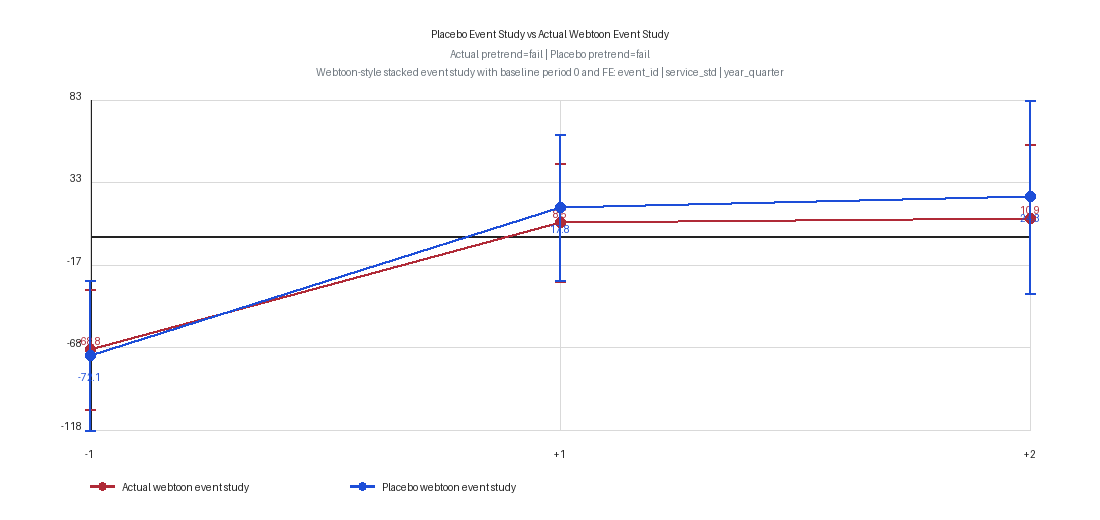
\includegraphics[width=0.88\textwidth]{outputs/figures/claim_strengthening/F_claim_placebo_event_plot.png}
\caption{위약 사건과 실제 사건의 사건연구 비교도}
\label{fig:claim_placebo_event}
\end{figure}

\section{비교사례의 관측 범위}
한국시장 확장 방향점수는 세 분야 모두 양수이고, 본문의 관측축 제외·가중치 변경에서도 그 방향이 유지된다. 별도로 적용한 엄격한 종합 판정기준은 자료의 직접성, 비교 가능성, 대체 설명까지 요구한다. 이 기준을 모두 충족한 직접 비교행은 0개였으며, 모든 분야에 일반화하는 강한 결론의 판정기준은 검토한 모든 시나리오에서 충족되지 않았다. 방향의 반복성이 확인되었다는 결과와 인과적 일반화에 필요한 자료가 더 있다는 판단은 이처럼 평가 대상이 다르다.

웹툰 및 스토리의 사례는 핵심축 관측이 적다. 또한 \nolinkurl{spotify@kr}, \nolinkurl{youtube_music@kr}, \nolinkurl{apple_music@kr}, \nolinkurl{netflix@kr}의 동일 서비스 직접 부담자료에는 결측 또는 범위값만 제시된 항목이 있다. 인프라의 위험-회수 축은 KT에서 양수, SK Telecom·LG Uplus에서 음수다. 따라서 정책은 종합점수와 함께 기업·채널별 부담을 확인해야 한다. 공식 요금 공시와 공정거래위원회의 유튜브 결합상품 시정자료는 해당 상품·집행 사실을 확인하는 별도의 근거다.

음악 확장 분석에서 공개자료로 확인한 항목과 추가 자료가 필요한 항목은 다음과 같다.

\begingroup
\footnotesize
\begin{summarylist}
  \item \textbf{라이선스 공개식 비중 격차}. 상태: 자료공개 여부의 코딩. 값: 1.000. 해석: 검토한 자료에서 국내 기준식과 해외 계약식의 공개범위가 다르다.
  \item \textbf{멜론 대 스포티파이 투명성 격차}. 상태: 투명성 항목의 연구 코딩. 값/경계: 4. 해석: 검토한 상품·계약자료의 공개범위 차이를 항목 수로 정리한 값이다.
  \item \textbf{멜론 대 유튜브 뮤직 투명성 격차}. 상태: 투명성 항목의 연구 코딩. 값/경계: 4. 해석: 유사 음원상품 비교의 자료공개 차이를 정리한 값이다.
  \item \textbf{법인 회계상 유효세율 차이}. 상태: 공시 추출값의 산술 비교. 값: 0.379(약 37.9\%p). 해석: FY2025 Dreamus와 Spotify 법인의 법인세비용/세전이익 차이다. 같은 회계연도의 비교이며, 한국 음악서비스의 현금세부담 귀착을 확인하려면 연결범위·이연법인세·서비스별 배분자료가 필요하다.
  \item \textbf{실제 해외 라이선스 요율 격차}. 상태: 미식별. 값/경계: --. 해석: 해외 계약 원문, 분모, 결합상품 범위 조정이 공개되지 않는다.
  \item \textbf{한국 대상 해외 상품 세부담 귀착 격차}. 상태: 미식별. 값/경계: --. 해석: 상품 단위 한국 세금 행과 법인-상품 배분 기준이 없다.
\end{summarylist}
{\par\raggedright\footnotesize 주: 투명성 격차는 공개범위를 연구 코딩규칙으로 정리한 값이다. 실제 해외 라이선스 요율과 한국 대상 상품의 세부담 귀착을 확인하려면 계약 및 서비스별 배분자료가 필요하다. 공개범위의 차이만으로 탈세 여부나 세금 회피 규모를 판정할 수 없다.\par}
\endgroup

\section{대체 설명과 후속 자료}
규모, 품질, 브랜드, 관측시점과 자료 가용성은 부담 차이에 영향을 줄 수 있다. 다음은 각 설명을 현재 분석에서 얼마나 줄였는지에 대한 점검 결과다. 잔여위험이 있다는 판정은 해당 요인이 관측된 차이의 일부를 설명할 가능성이 남아 있다는 뜻이다.

\begingroup
\small
\begin{summarylist}
  \item \textbf{단순 규모 차이}. 상태: 부분 축소. 잔여위험: 높음.
  \item \textbf{서비스 품질 차이}. 상태: 미해소. 잔여위험: 높음.
  \item \textbf{브랜드 및 네트워크 효과 차이}. 상태: 미해소. 잔여위험: 높음.
  \item \textbf{시기 차이}. 상태: 부분 축소. 잔여위험: 중간.
  \item \textbf{국가별 거시환경 차이}. 상태: 부분 축소. 잔여위험: 중간.
  \item \textbf{상장사·비상장사 공시 가용성 차이}. 상태: 미해소. 잔여위험: 높음.
  \item \textbf{제품 범위 차이}. 상태: 상당 축소. 잔여위험: 중간.
  \item \textbf{비교군 매칭 실패 또는 비교단위 불일치}. 상태: 부분 축소. 잔여위험: 중간.
  \item \textbf{proxy 및 측정오차 가설}. 상태: 미해소. 잔여위험: 높음.
\end{summarylist}
{\par\raggedright\footnotesize 주: 전체 분포는 \texttt{substantially\_reduced 1}, \texttt{partially\_reduced 4}, \texttt{still\_open 4}이며, \nolinkurl{can_still_weaken_claim=yes}는 \texttt{9/9}다.\par}
\endgroup

비공개 계약조건, 추천·노출 기준, 실시간 거래자료는 공개자료만으로 확인하기 어렵다. 후속 수집에서는 서비스별 비용·정산자료와 품질·전환·유지율 자료를 같은 시장·기간으로 맞추어, 이들 요인이 부담 차이를 얼마나 설명하는지 검증한다.



\end{document}
